\cvevent{\printinfo{\faPlusSquare}{빌더허브 플랫폼 개발 B2C}}{(주)창소프트아이앤아이 개발리딩}{2022.06 -- now}{Seoul, Korea}

\begin{itemize}
\item 소개: 건축을 시작하기 위한 그리고 건축 관련 관계자들을 위한 허브
\item 1차 목표: 건축 견적 시장을 점유하여 플레이어들을 위한 서비스들을 만들어 플랫폼화
\item 참여 개발 내용: 플랫폼 개발 본부 리딩, 인프라 및 풀스택 플랫폼 서비스 구축
\item 개발 서비스
\begin{itemize}[label=$\star$]
	\item \href{https://builderhub.io}{홈 서비스} 개발
	      \begin{itemize}
		      \item 각 서비스들의 허브
		      \item 고객센터, 1:1문의, ChatOps, 설문조사 챗봇
		      \item CMS: Notion API(NextJS SSG\&SSR)
	      \end{itemize}
	      \begin{figure}[!ht]
		      \begin{fullwidth}
			      \parbox{0.35\textwidth}{
				      \centering
				      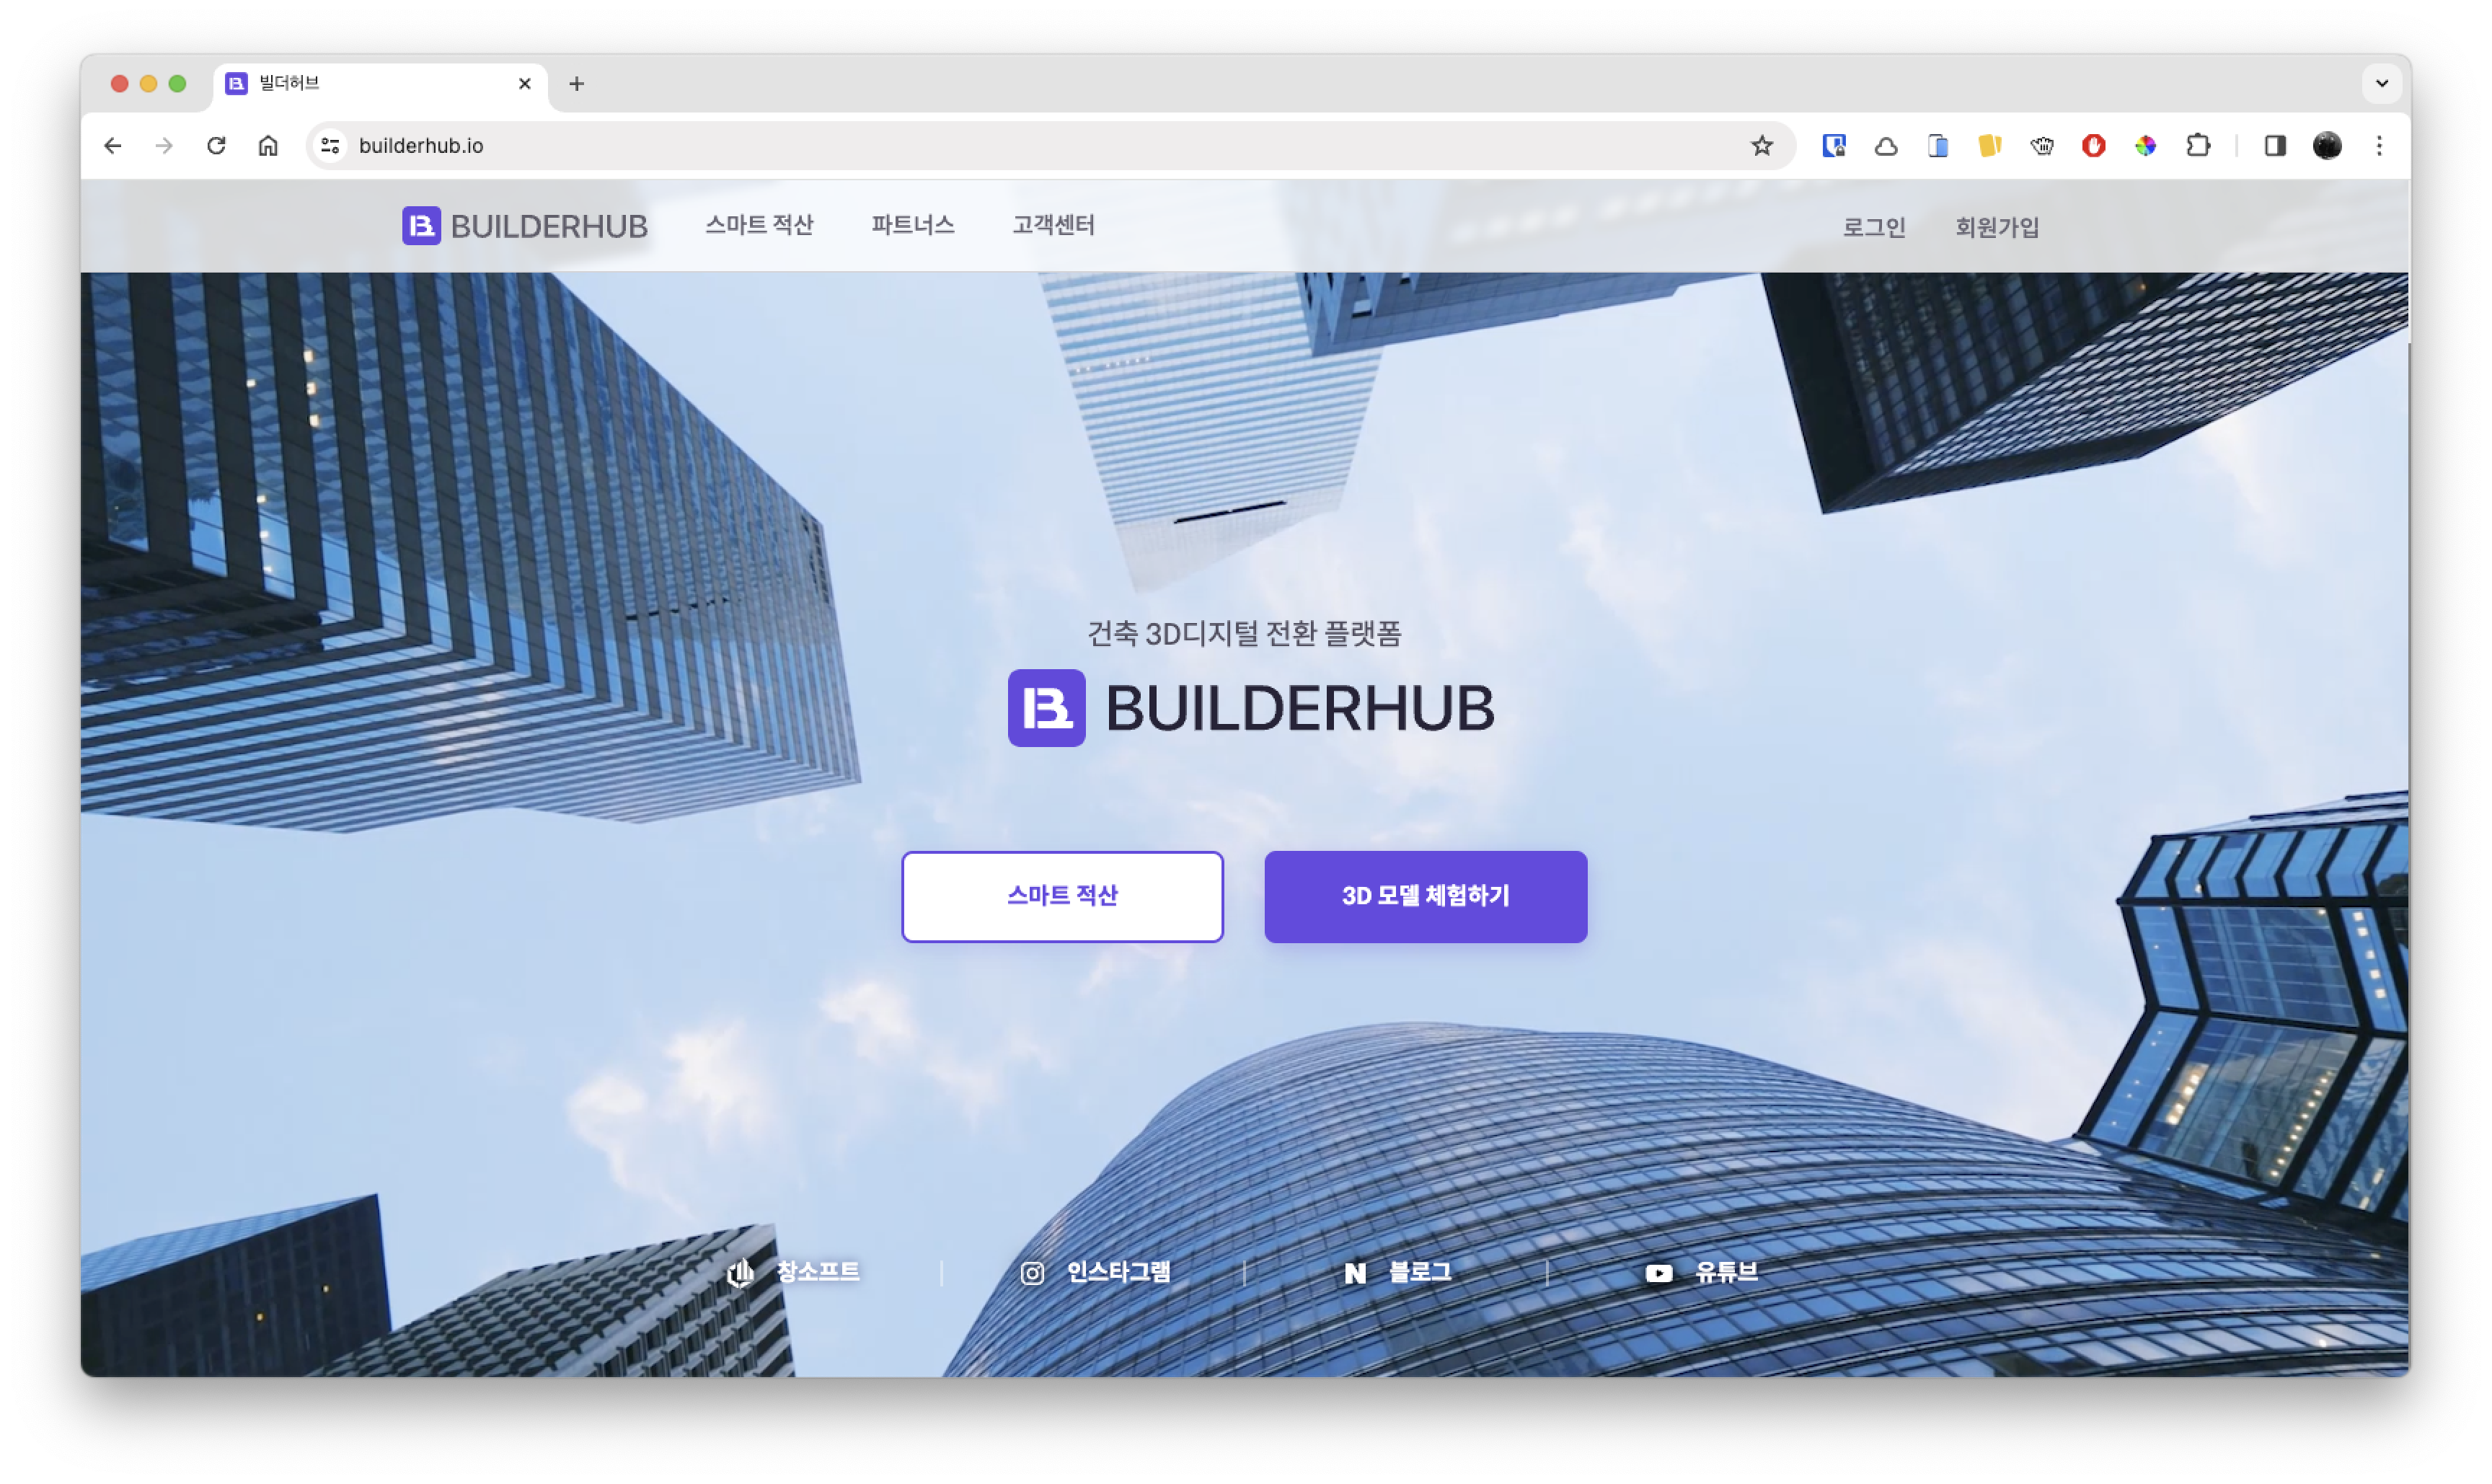
\includegraphics[width=0.35\textwidth]{images/builderhub-home-1.png}
				      \caption*{Builderhub}
			      }\qquad
			      \parbox{0.35\textwidth}{
				      \centering
				      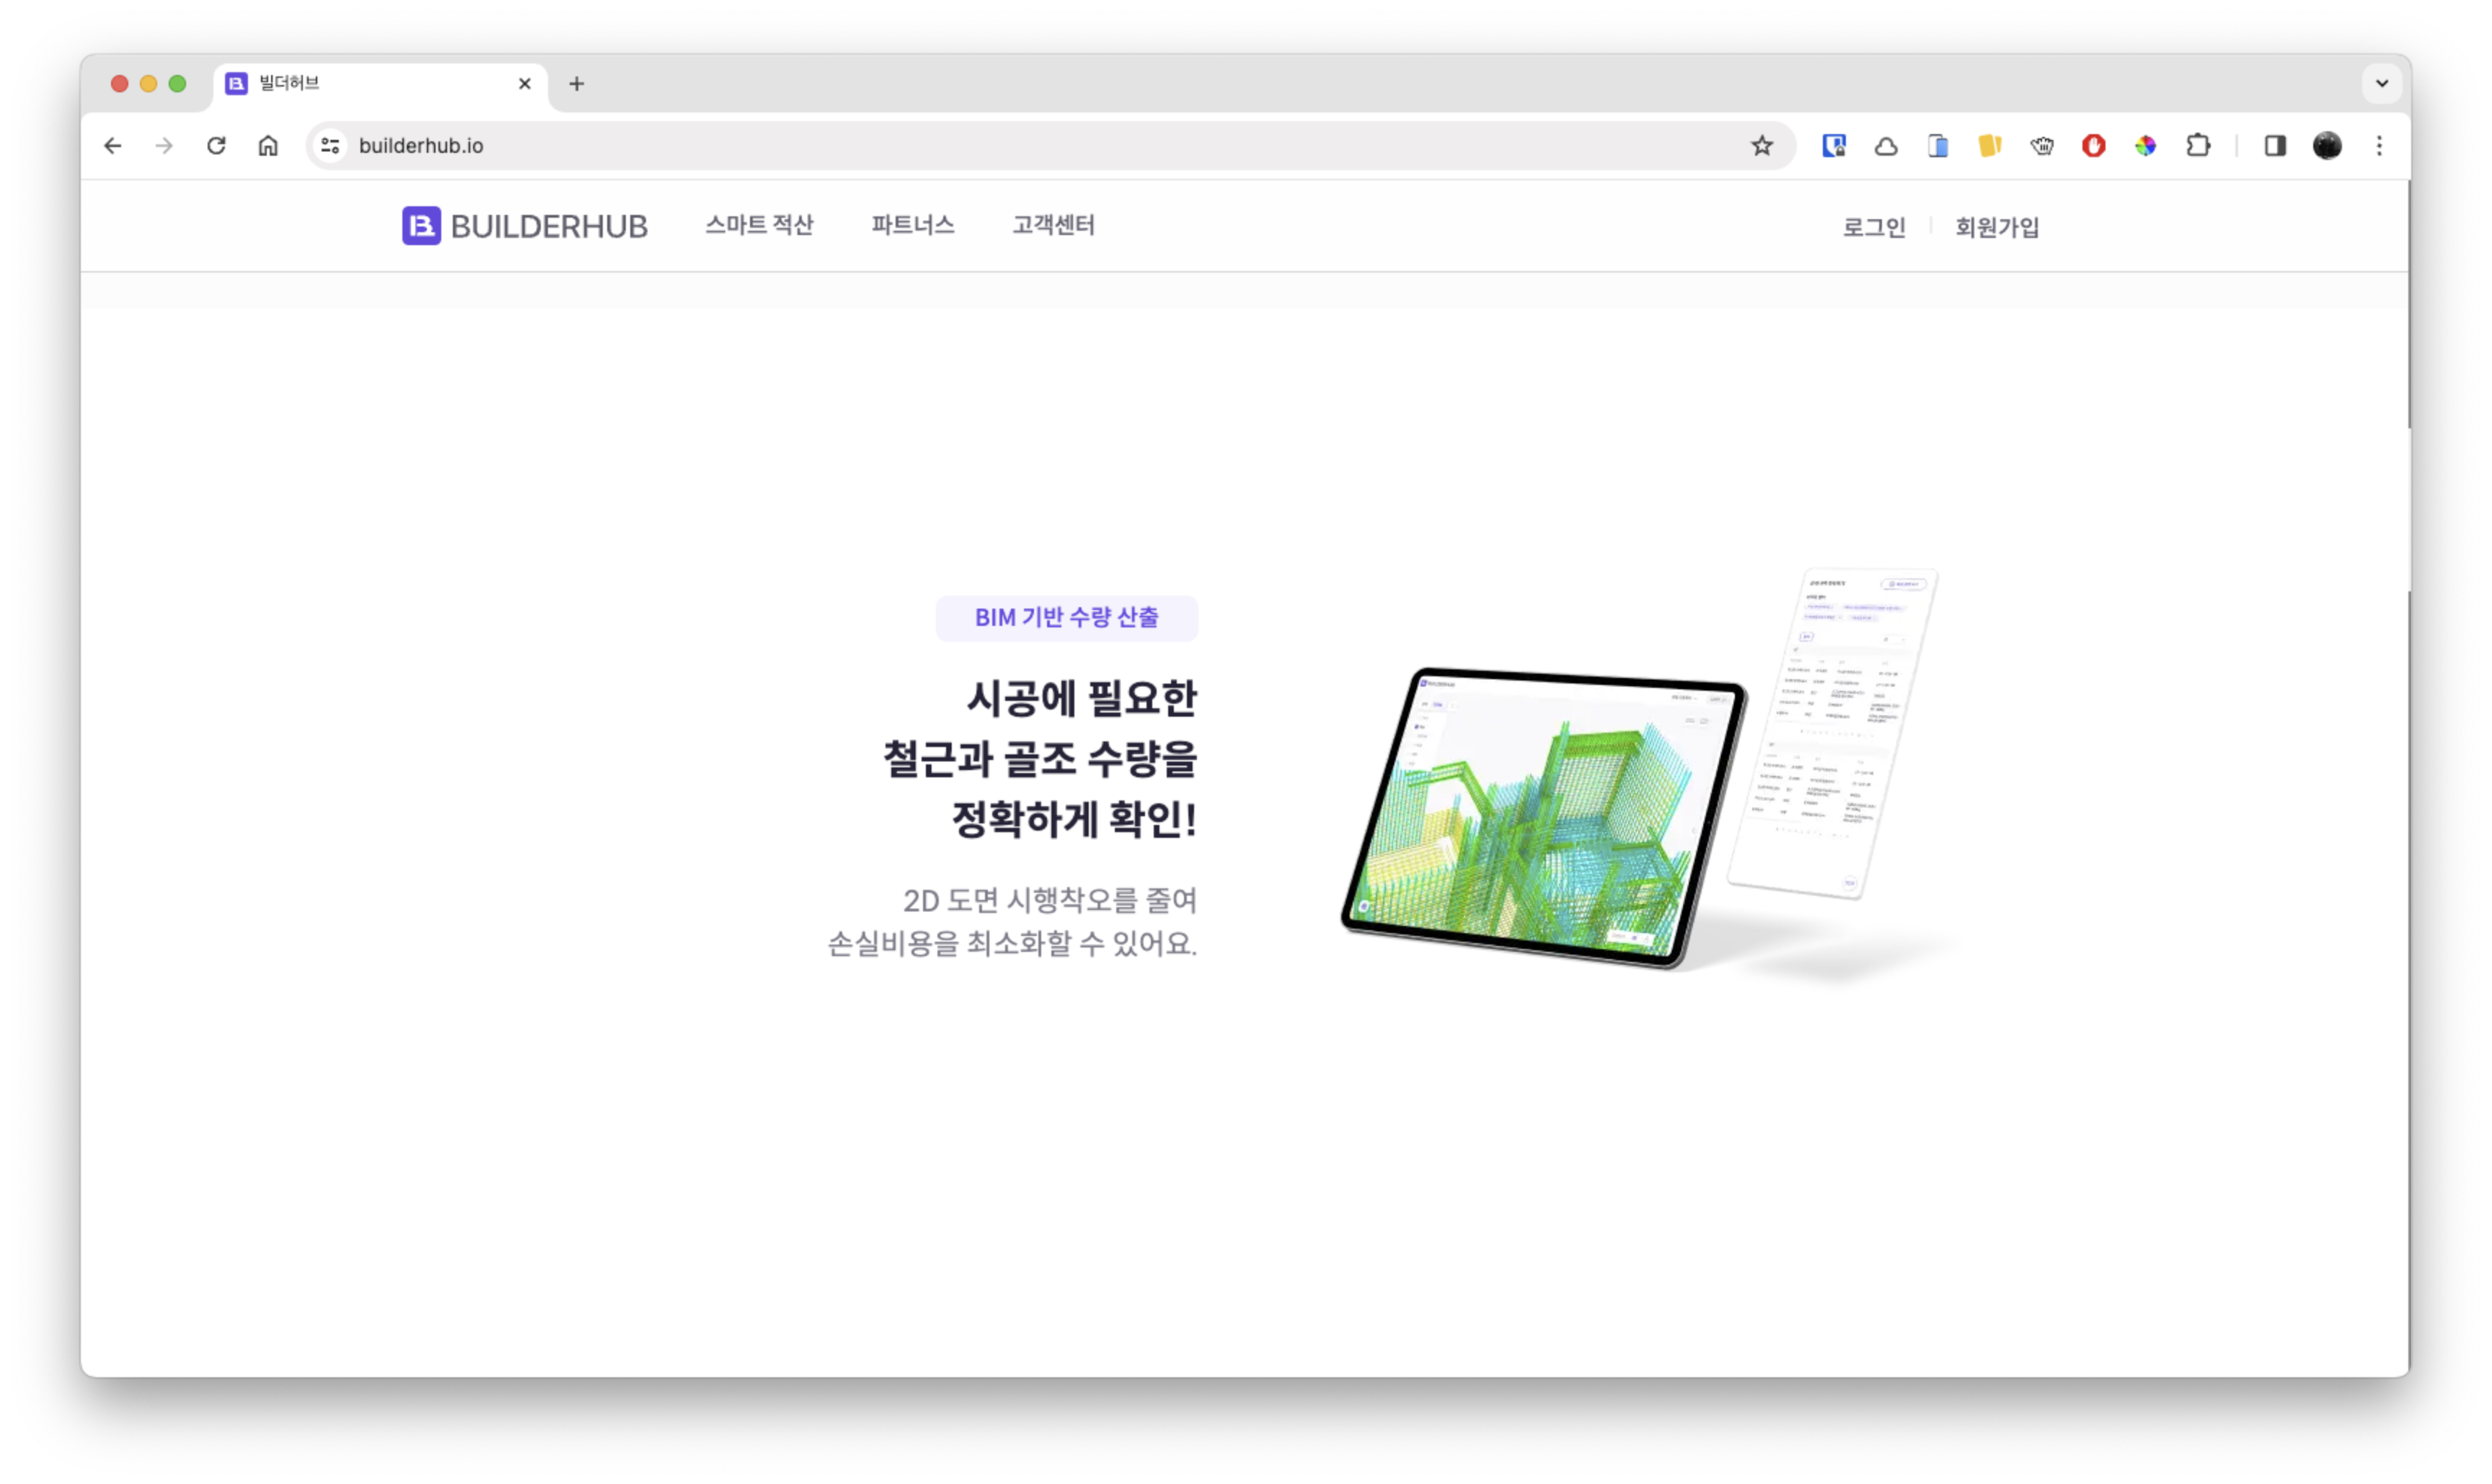
\includegraphics[width=0.35\textwidth]{images/builderhub-home-2.png}
				      \caption*{Home}
			      }\qquad
			      \parbox{0.35\textwidth}{
				      \centering
				      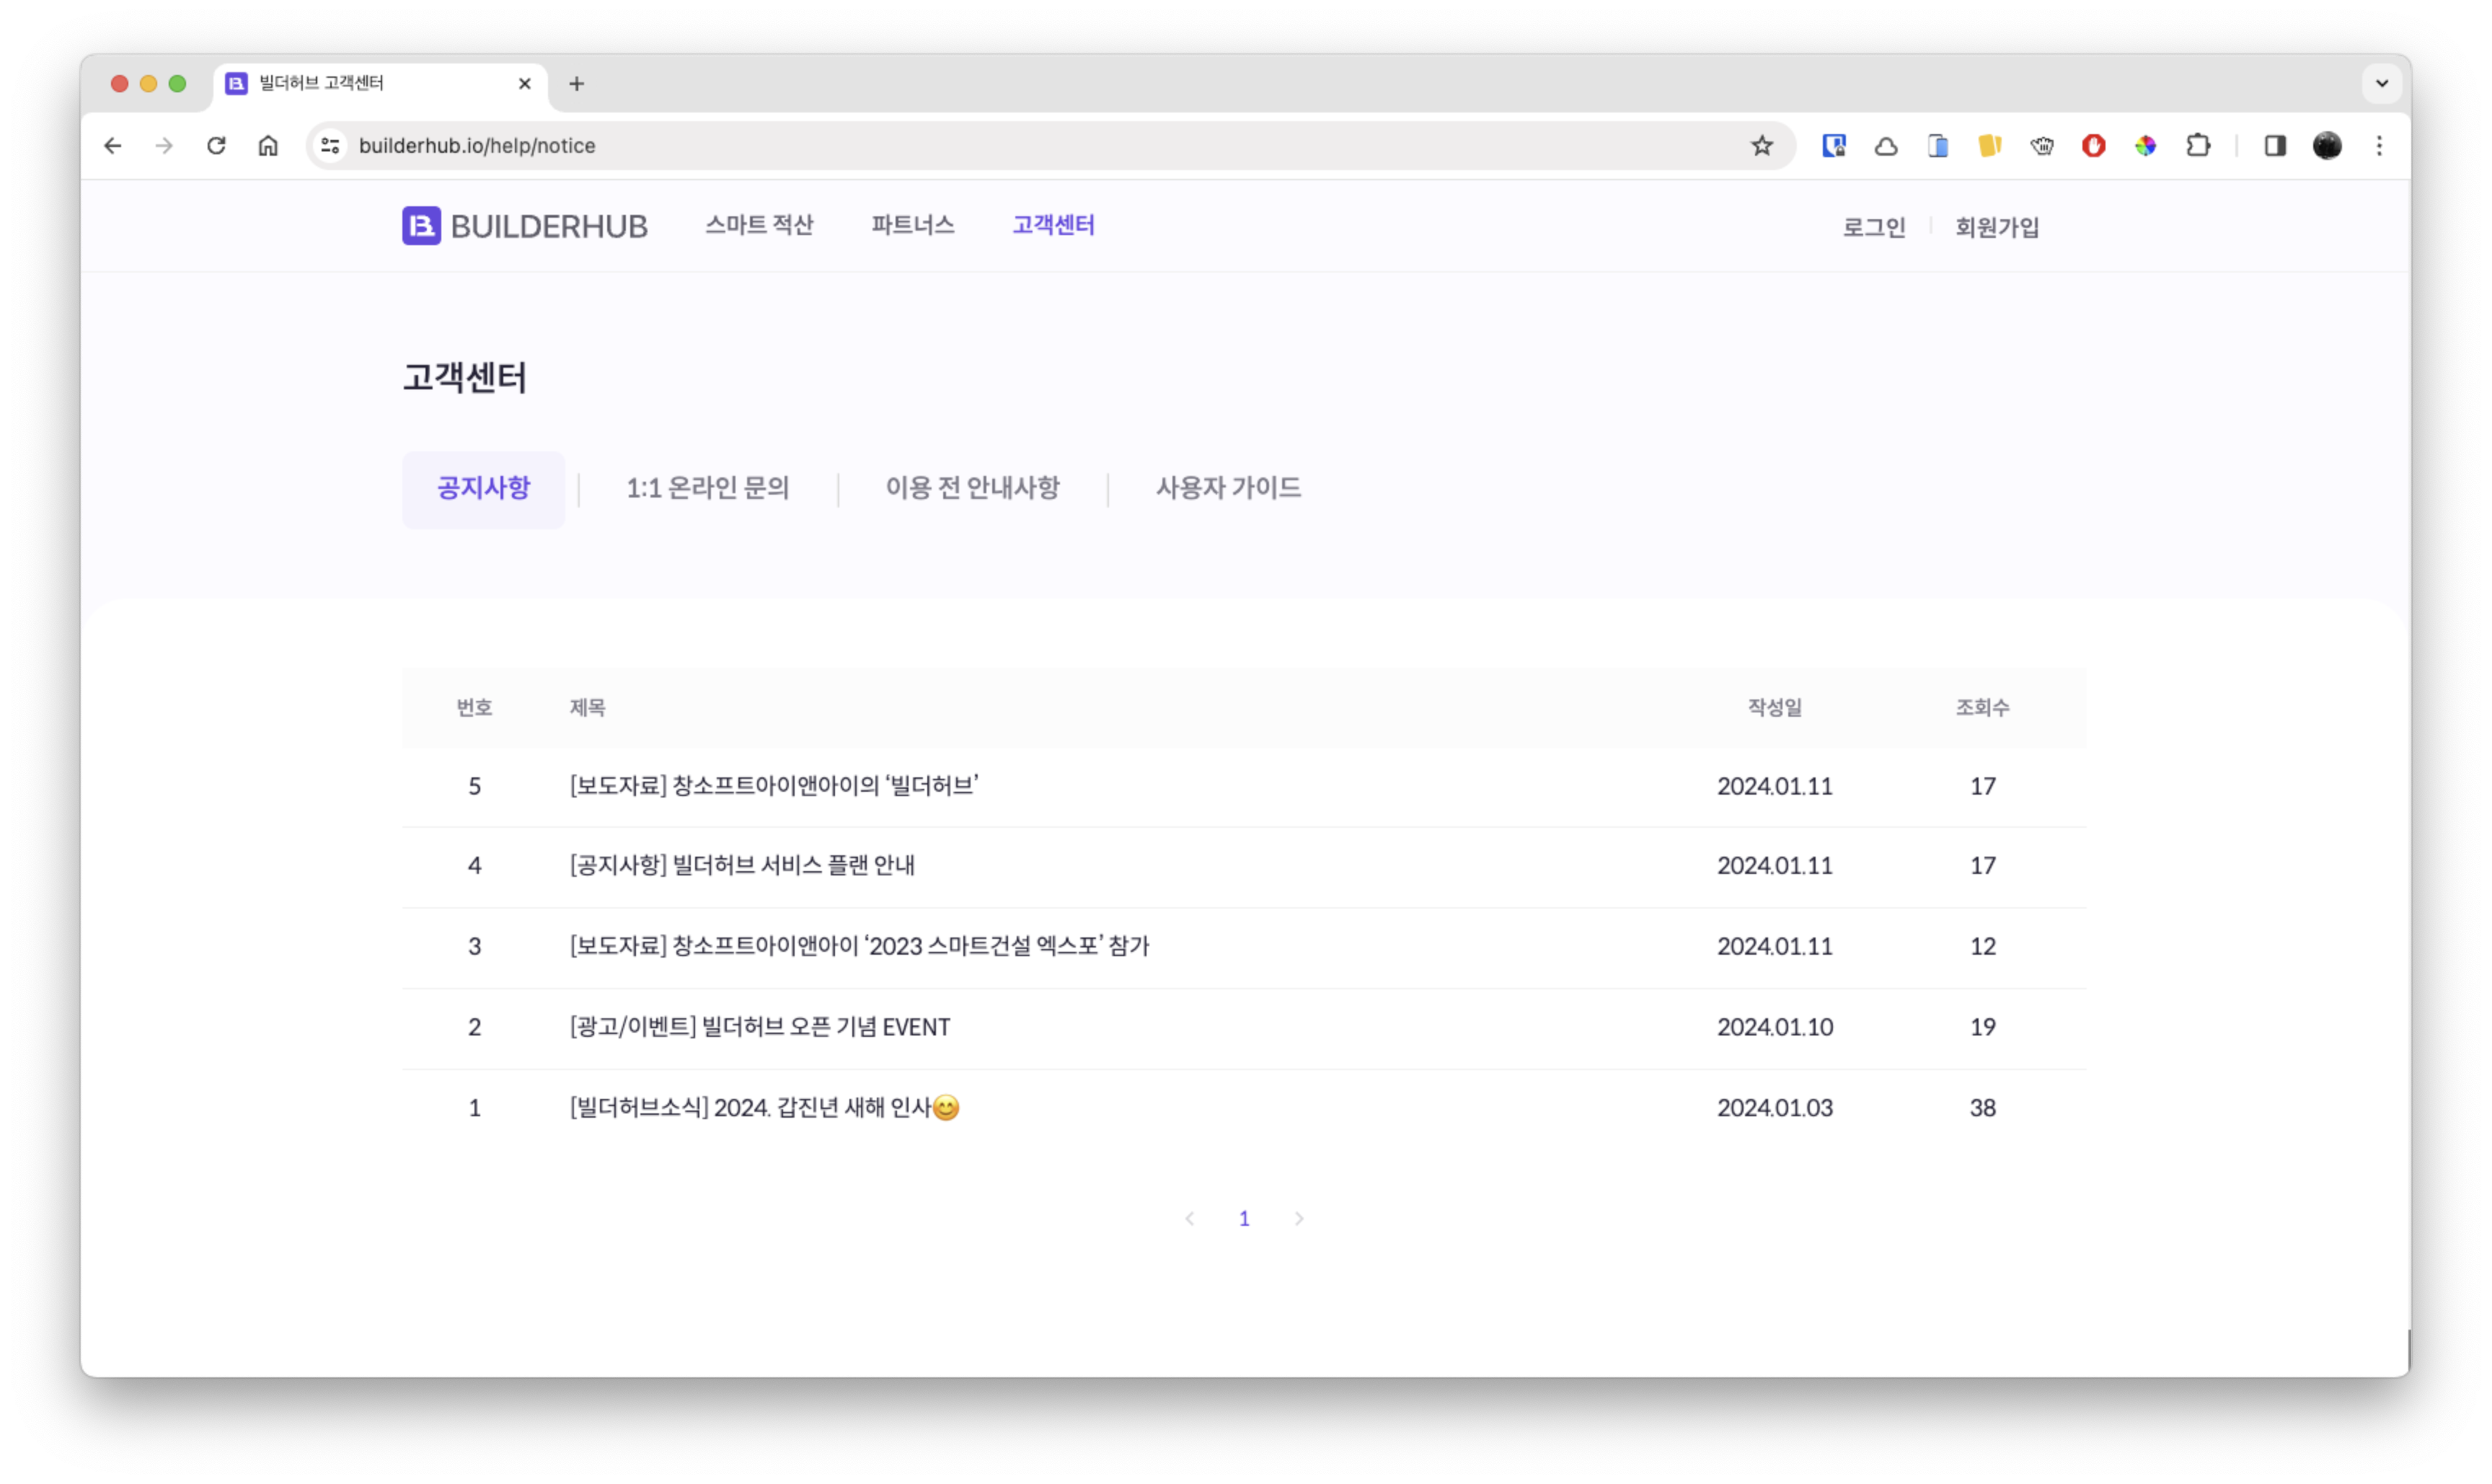
\includegraphics[width=0.35\textwidth]{images/builderhub-home-cs-1.png}
				      \caption*{1:1문의}
			      }\qquad
			      \parbox{0.35\textwidth}{
				      \centering
				      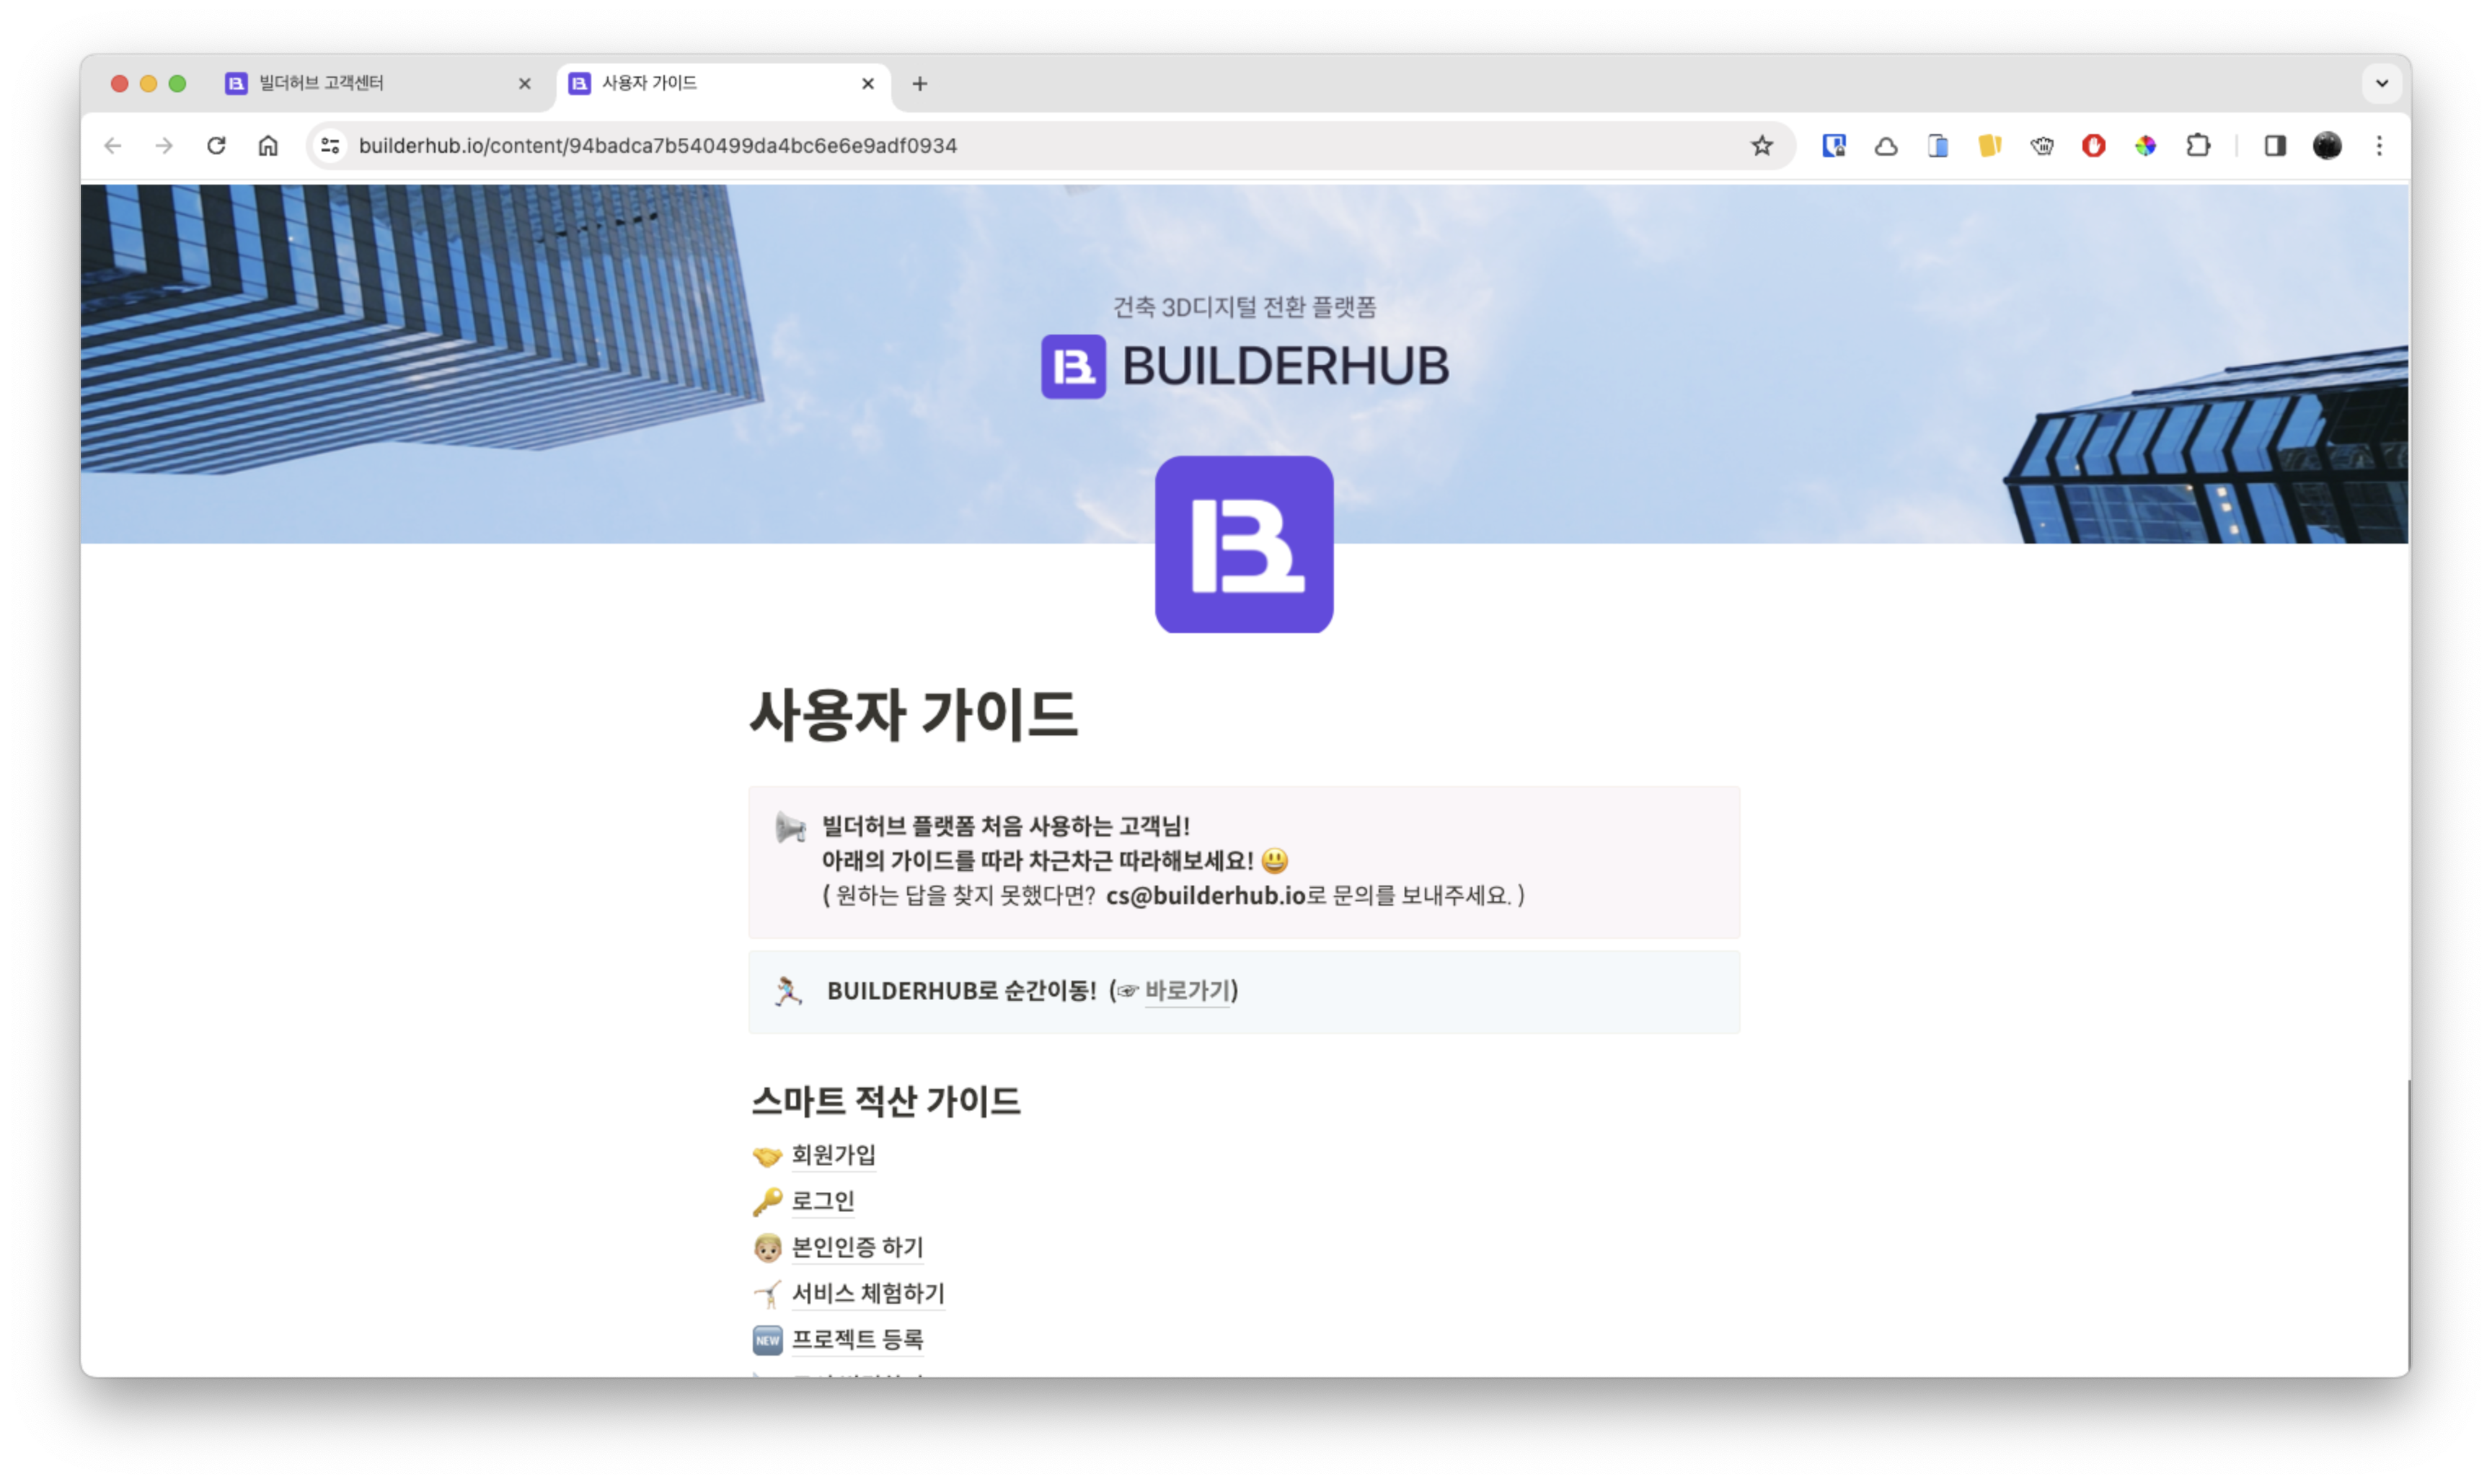
\includegraphics[width=0.35\textwidth]{images/builderhub-home-cs-2.png}
				      \caption*{Guide}
			      }
		      \end{fullwidth}
	      \end{figure}
	\item \href{https://auth.builderhub.io}{인증 서비스} 개발(회원가입, 로그인 세션, 마이페이지, 1:1문의 내역)
	      \begin{itemize}
		      \item 회원가입, 로그인
		      \item 로그인 세션 확인, 마이페이지, 1:1 문의 내역
		      \item SuperTokens(cIAM) API 커스텀, JWT \& Session 방식 인증\&인가, RBAC, OIDC
	      \end{itemize}
	      \begin{figure}[!ht]
		      \begin{fullwidth}
			      \parbox{0.5\textwidth}{
				      \centering
				      \includegraphics[width=0.5\textwidth]{images/builderhub-auth-1.png}
				      \caption*{Sign in}
			      }\qquad
			      \parbox{0.5\textwidth}{
				      \centering
				      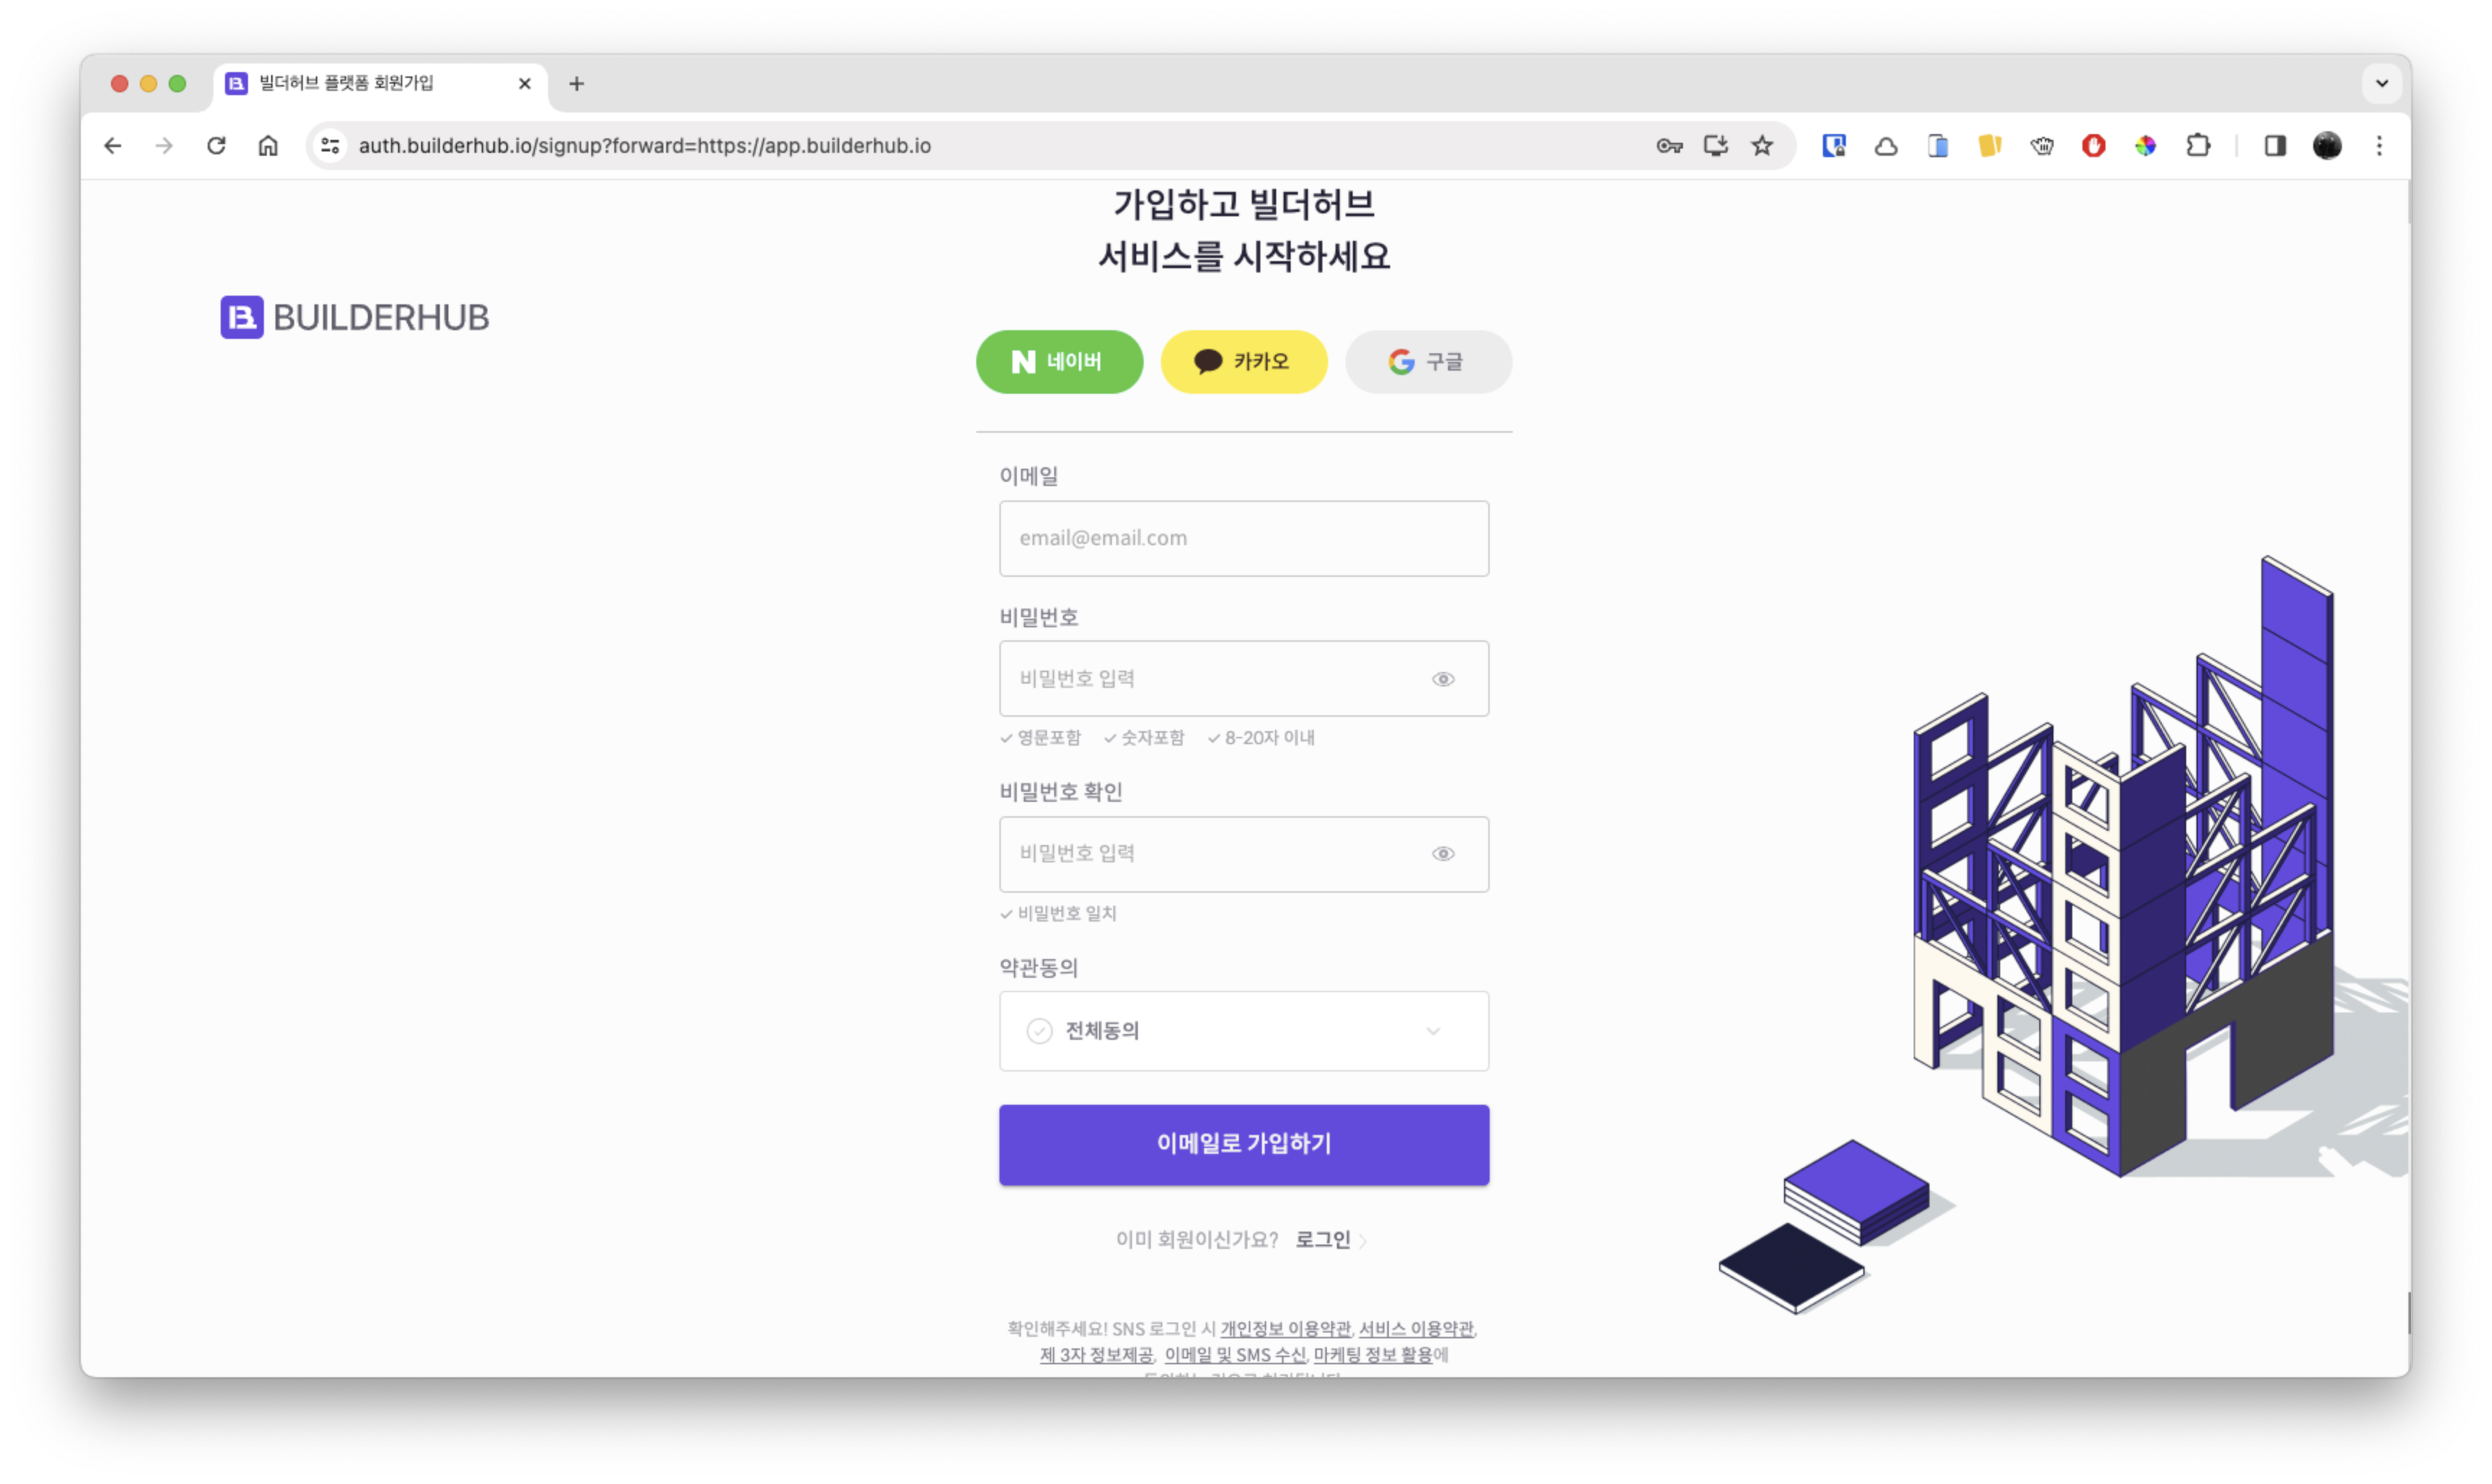
\includegraphics[width=0.5\textwidth]{images/builderhub-auth-2.png}
				      \caption*{Sign up}
			      }\qquad
			      \parbox{0.5\textwidth}{
				      \centering
				      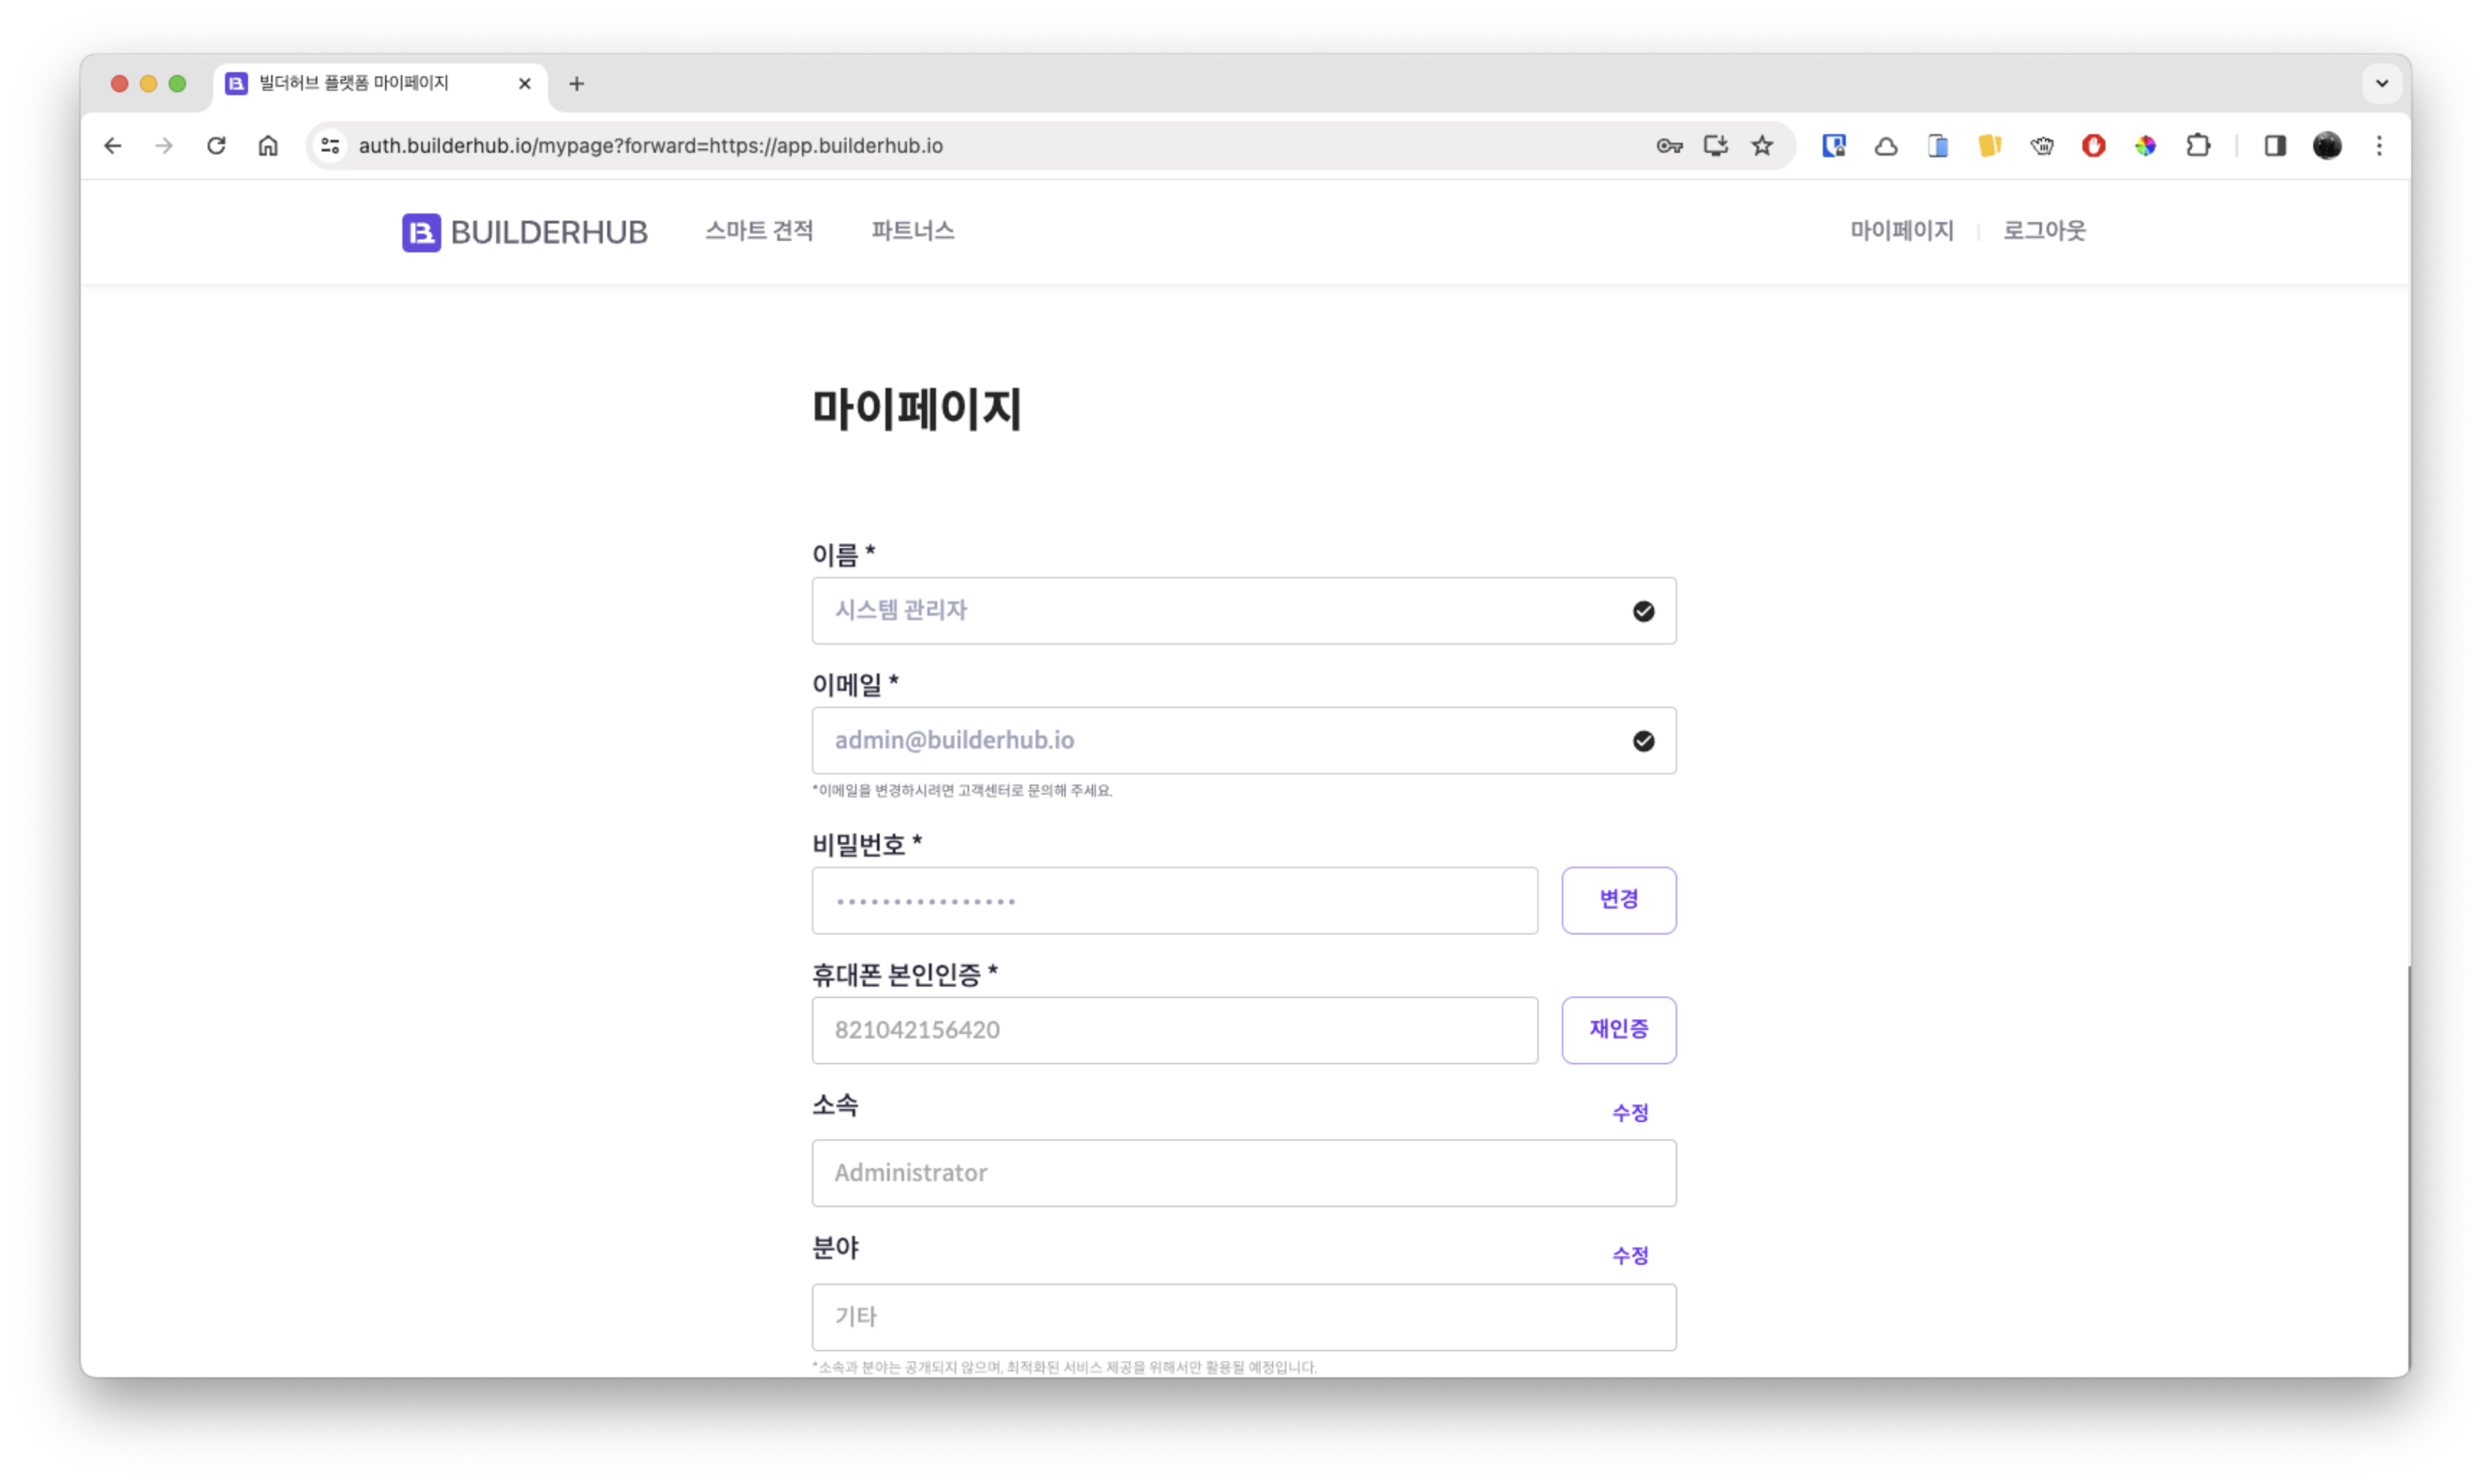
\includegraphics[width=0.5\textwidth]{images/builderhub-auth-mypage.png}
				      \caption*{My Page}
			      }
		      \end{fullwidth}
	      \end{figure}
	\item \href{https://app.builderhub.io}{커스터머 서비스} 개발
	      \begin{itemize}
		      \item 랜딩페이지, 프로젝트 리스트, 등록, 공유, 필터
		      \item 프로젝트 상태 확인, 결제 시스템, 알림톡 연동
		      \item 프로젝트 상세 확인, 변경 내역 히스토리
		      \item 표준내역서 관리, 내역화 (개발중)
	      \end{itemize}
	      \begin{figure}[!ht]
		      \begin{fullwidth}
			      \parbox{0.35\textwidth}{
				      \centering
				      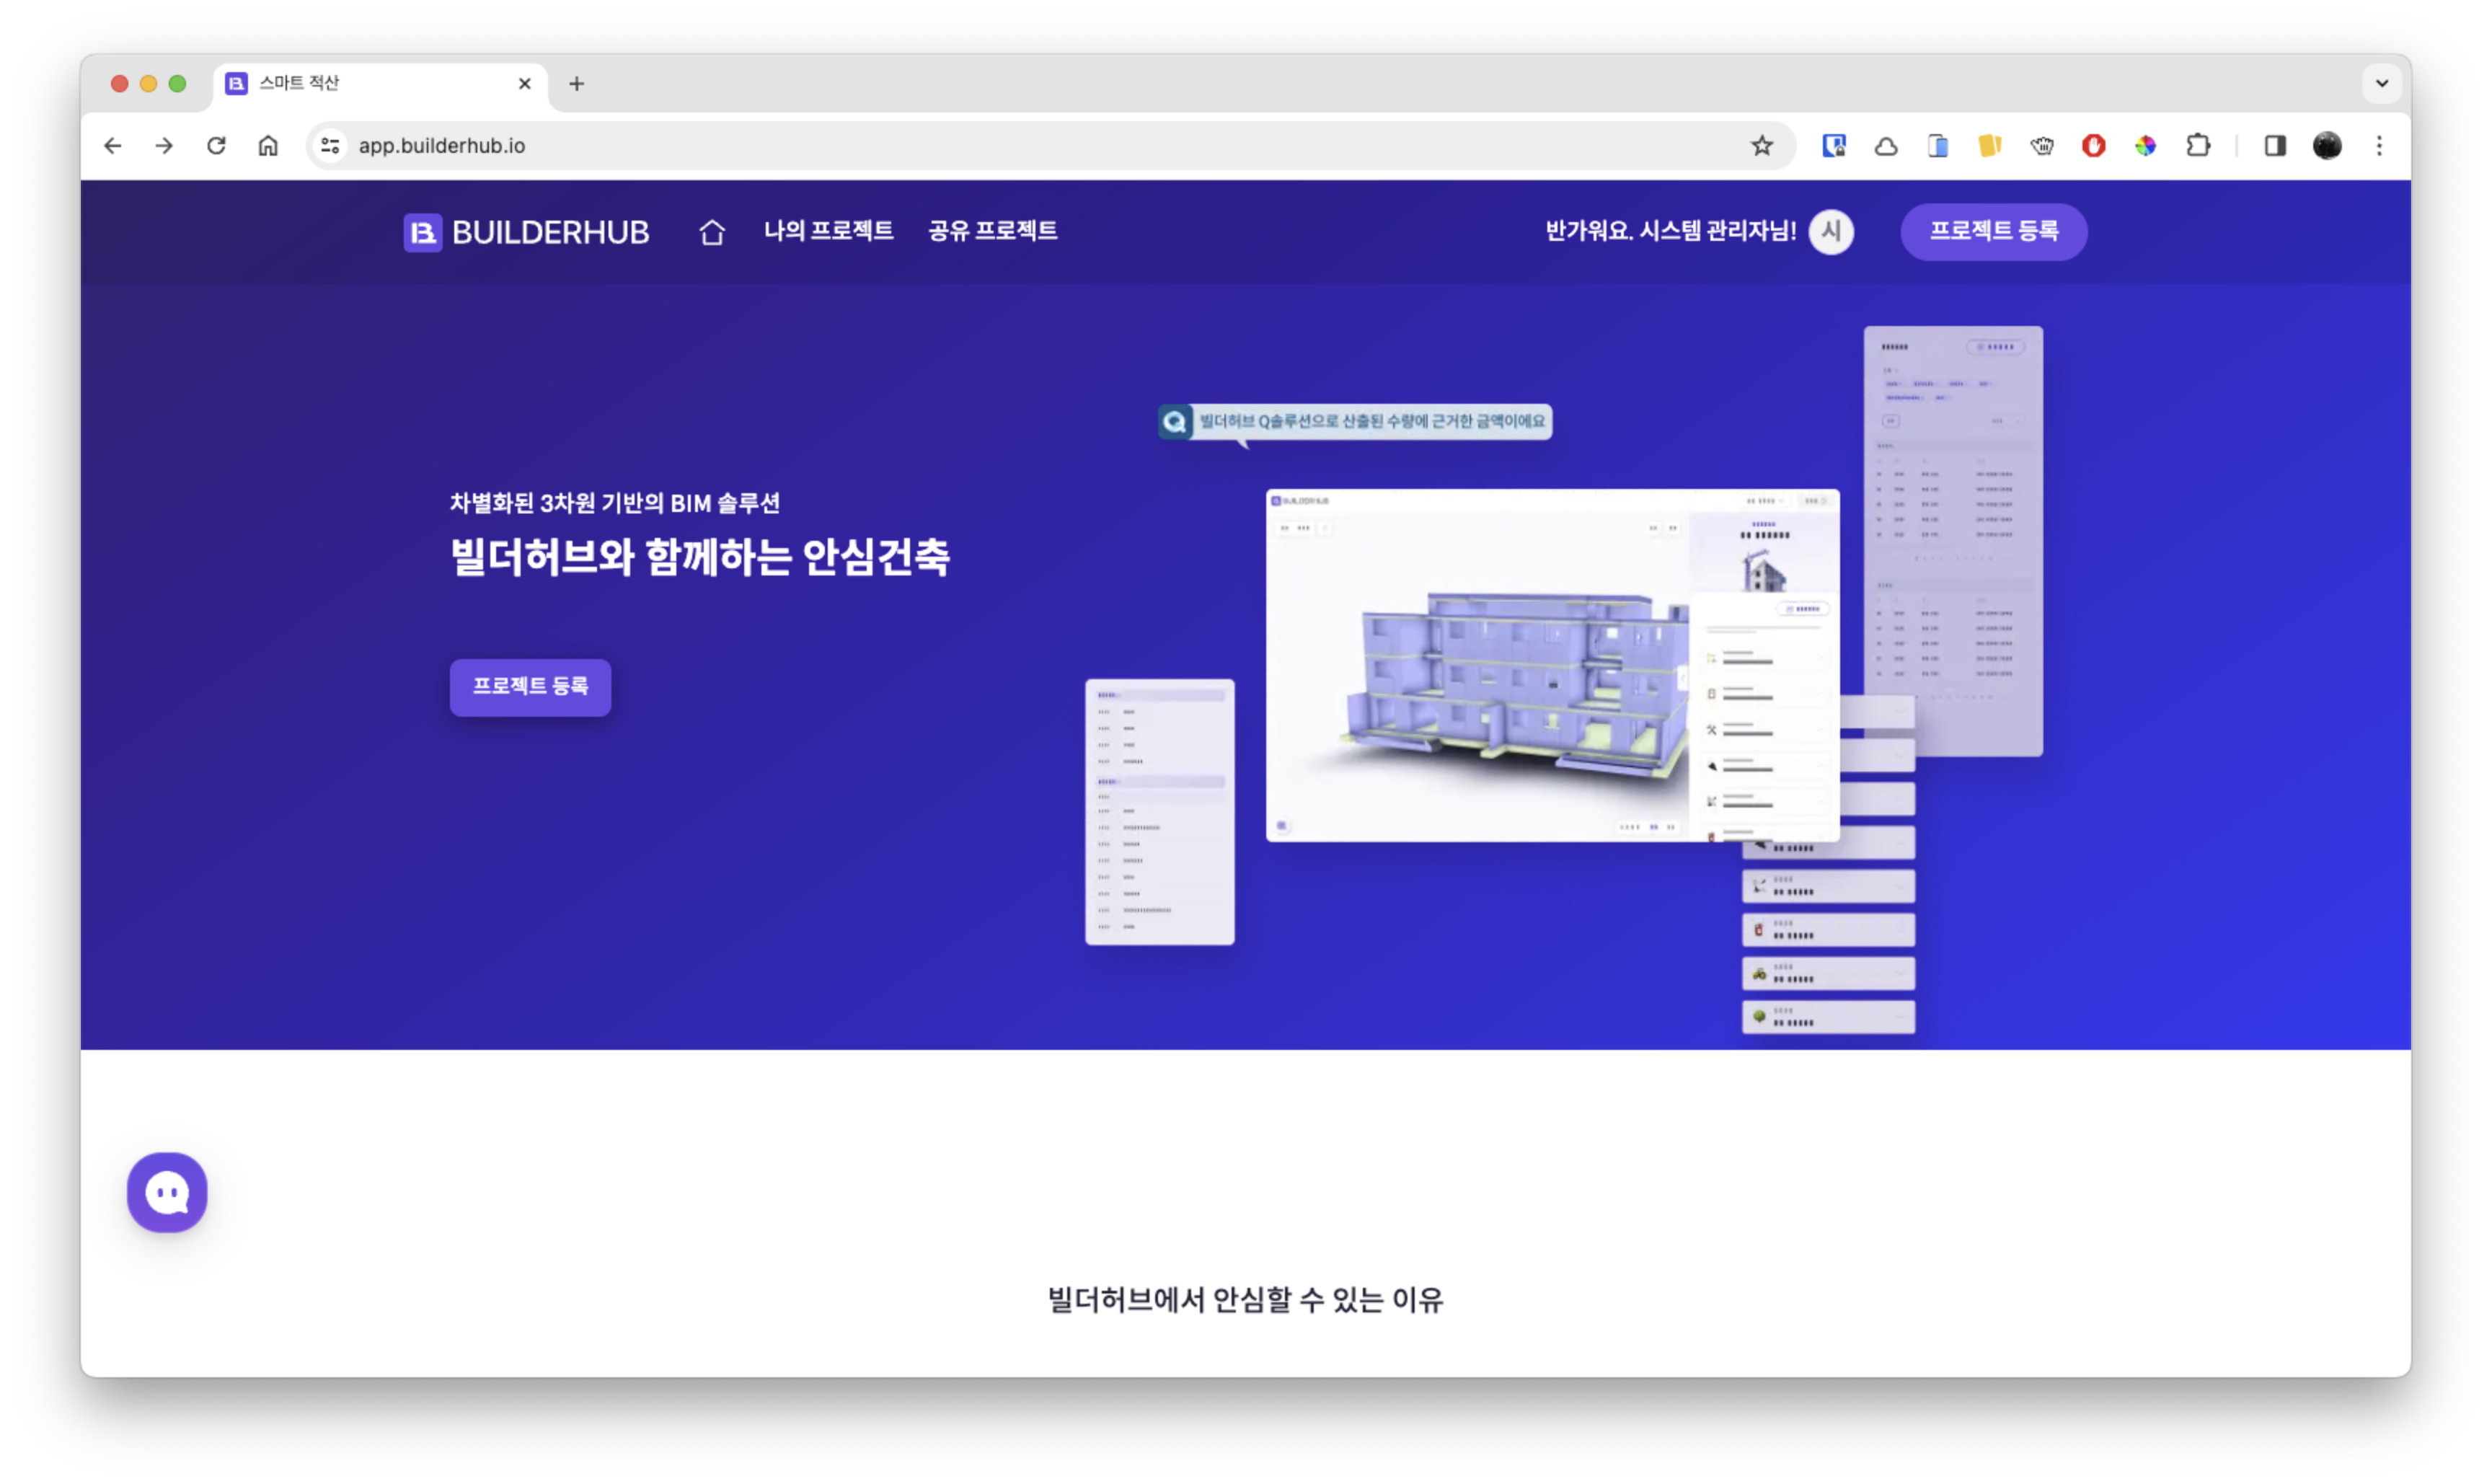
\includegraphics[width=0.35\textwidth]{images/builderhub-customer-1.png}
				      \caption*{Landing page}
			      }\qquad
			      \parbox{0.35\textwidth}{
				      \centering
				      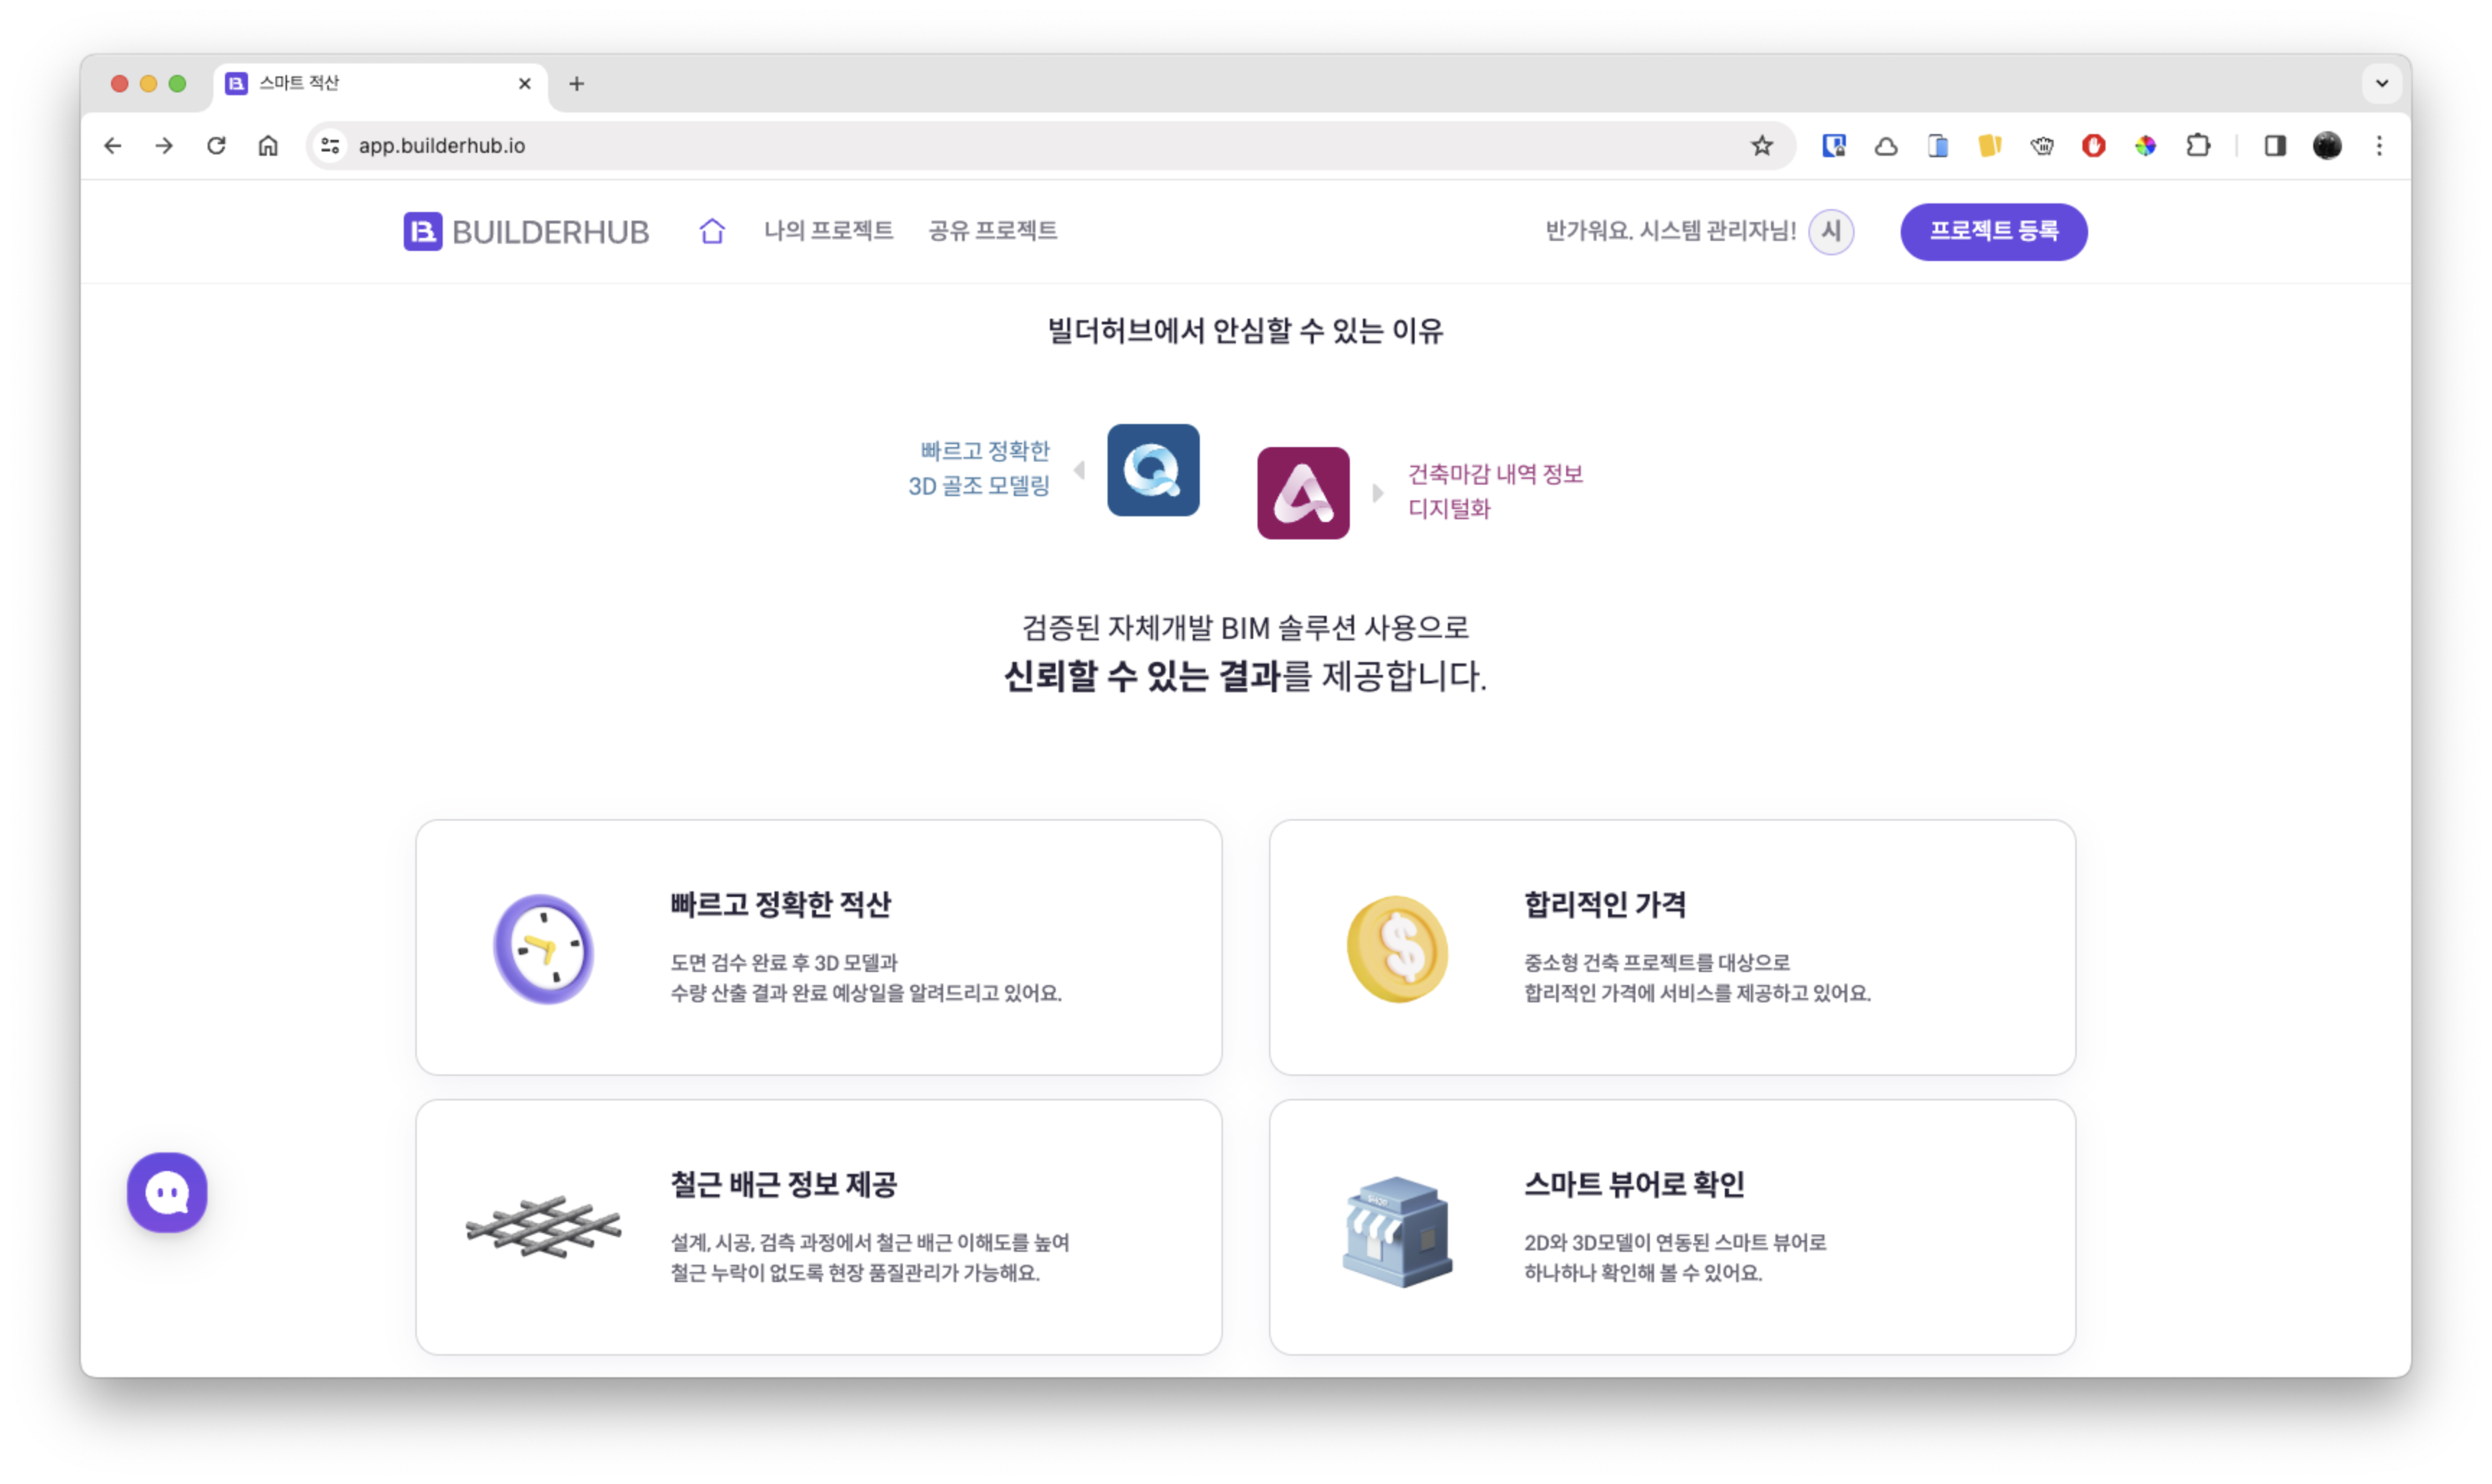
\includegraphics[width=0.35\textwidth]{images/builderhub-customer-2.png}
				      \caption*{Scroll base story telling}
			      }\qquad
			      \parbox{0.35\textwidth}{
				      \centering
				      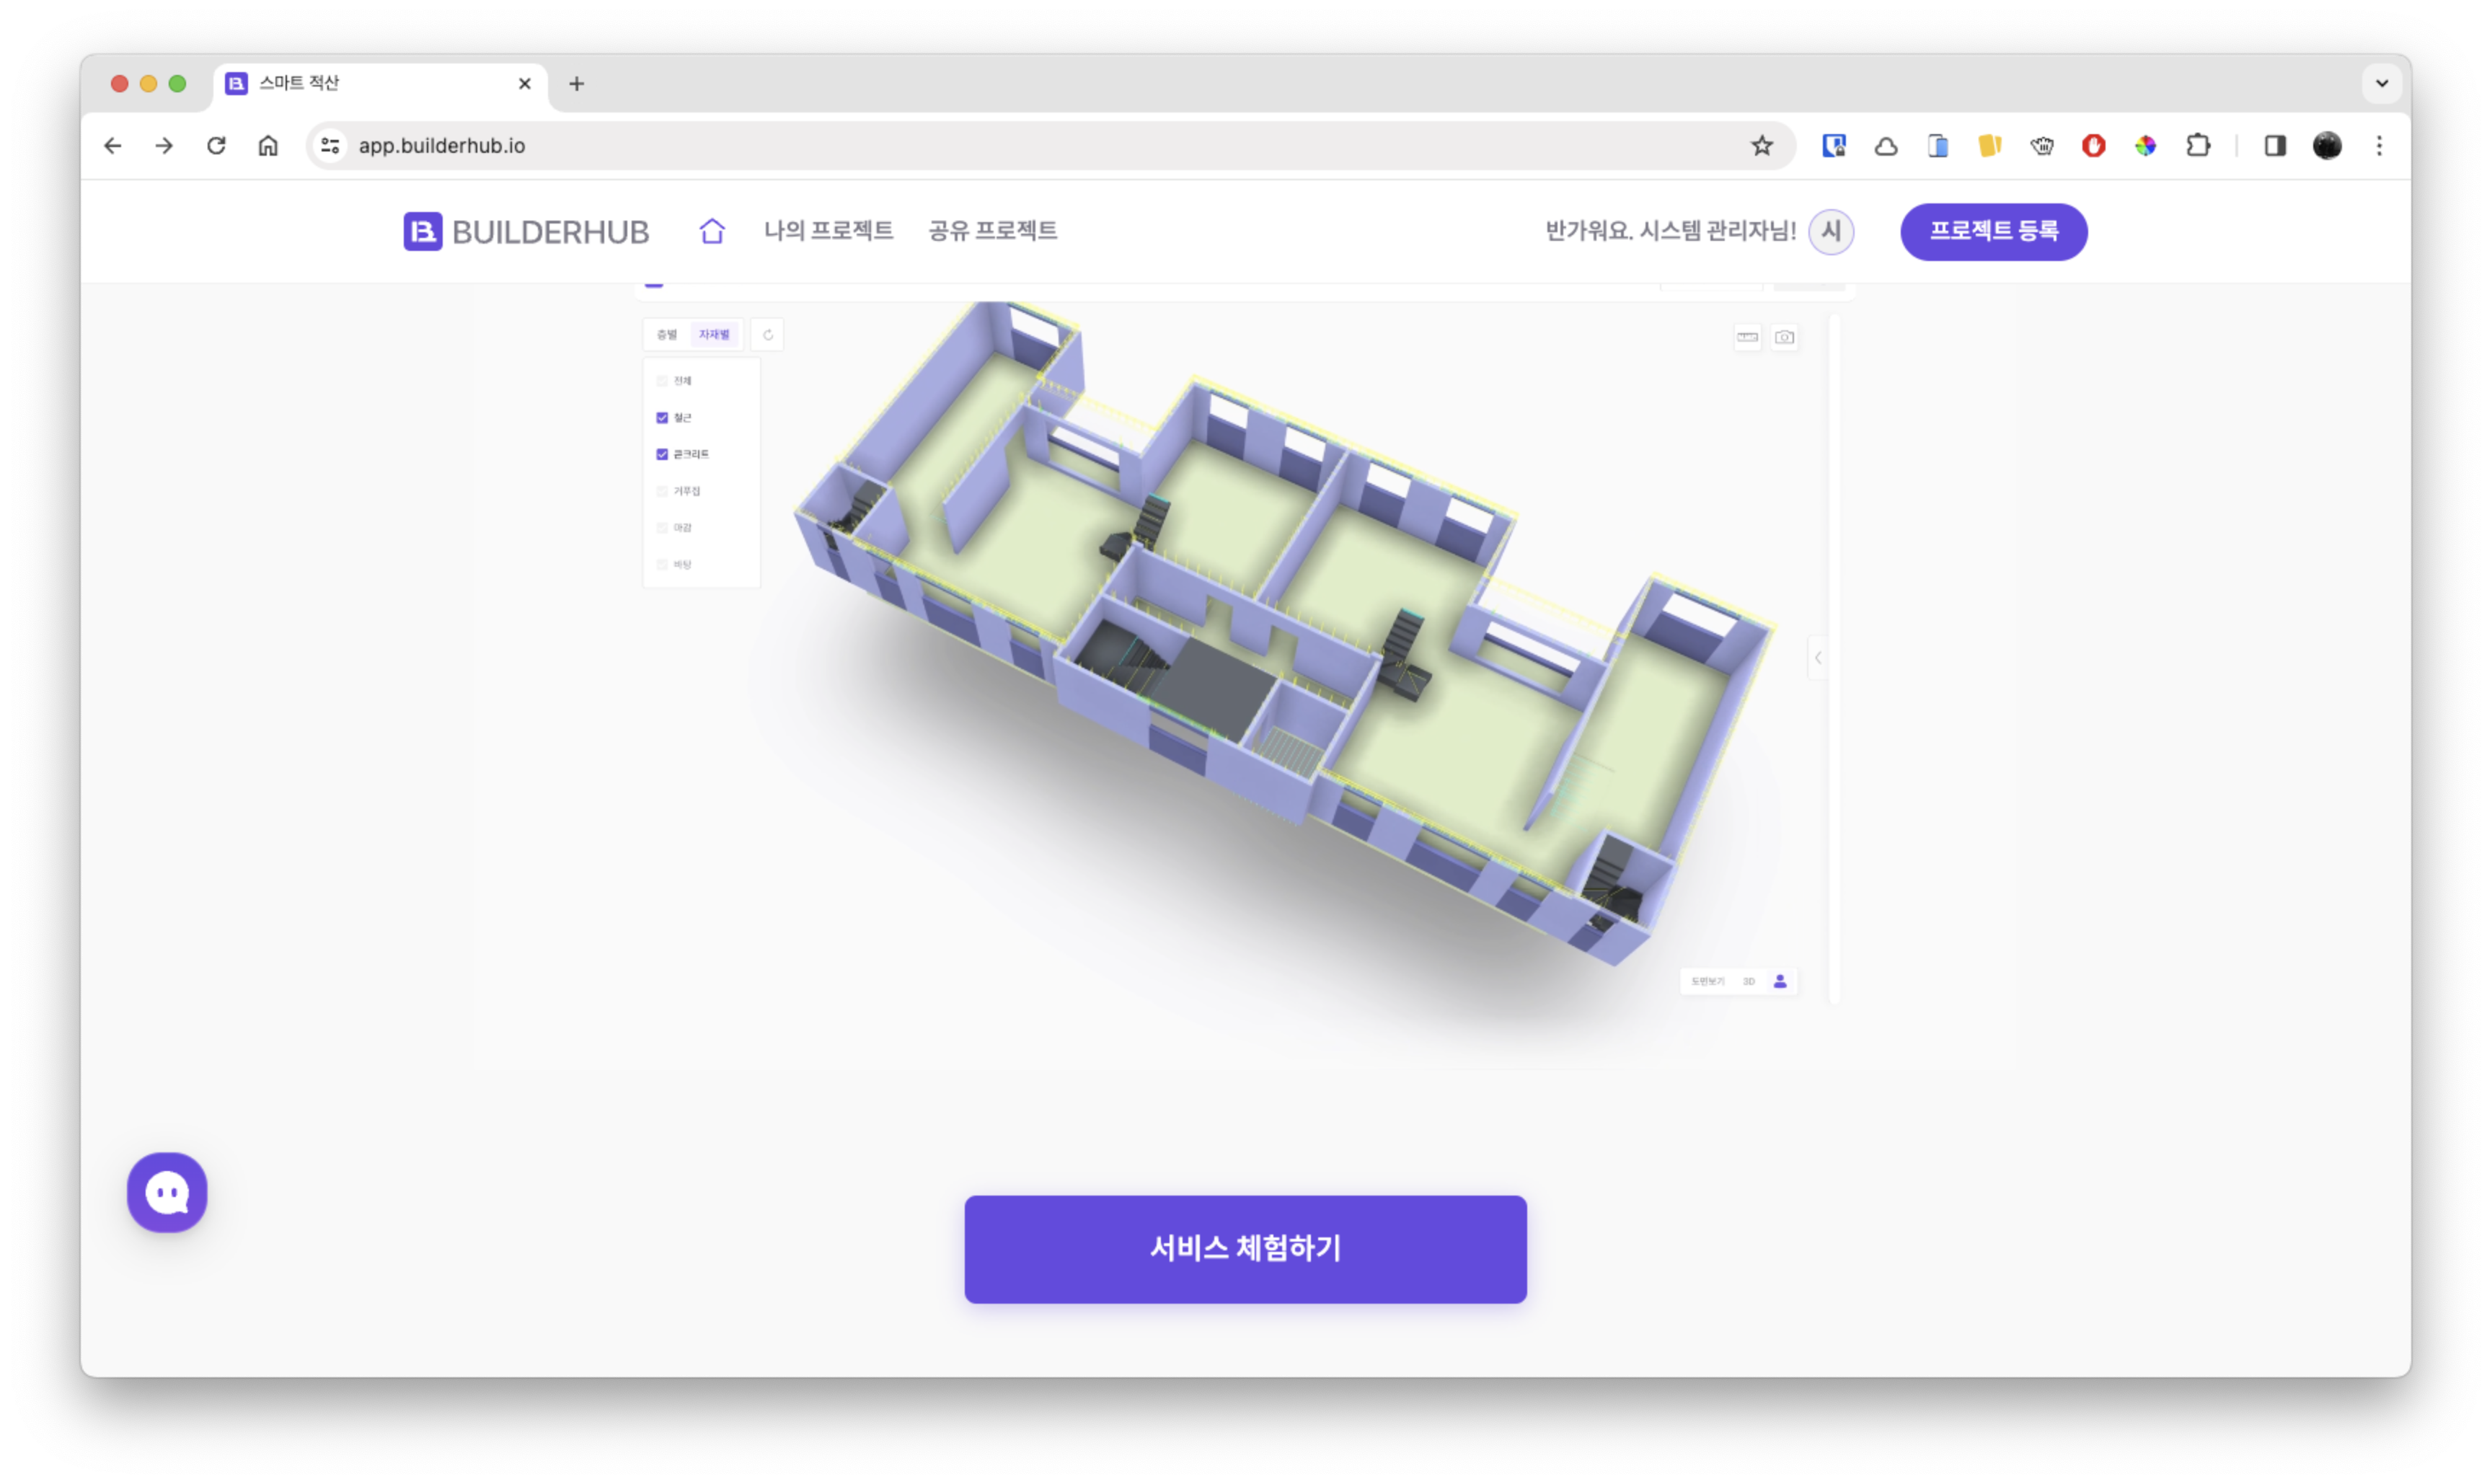
\includegraphics[width=0.35\textwidth]{images/builderhub-customer-3.png}
				      \caption*{Demo}
			      }\qquad
			      \parbox{0.35\textwidth}{
				      \centering
				      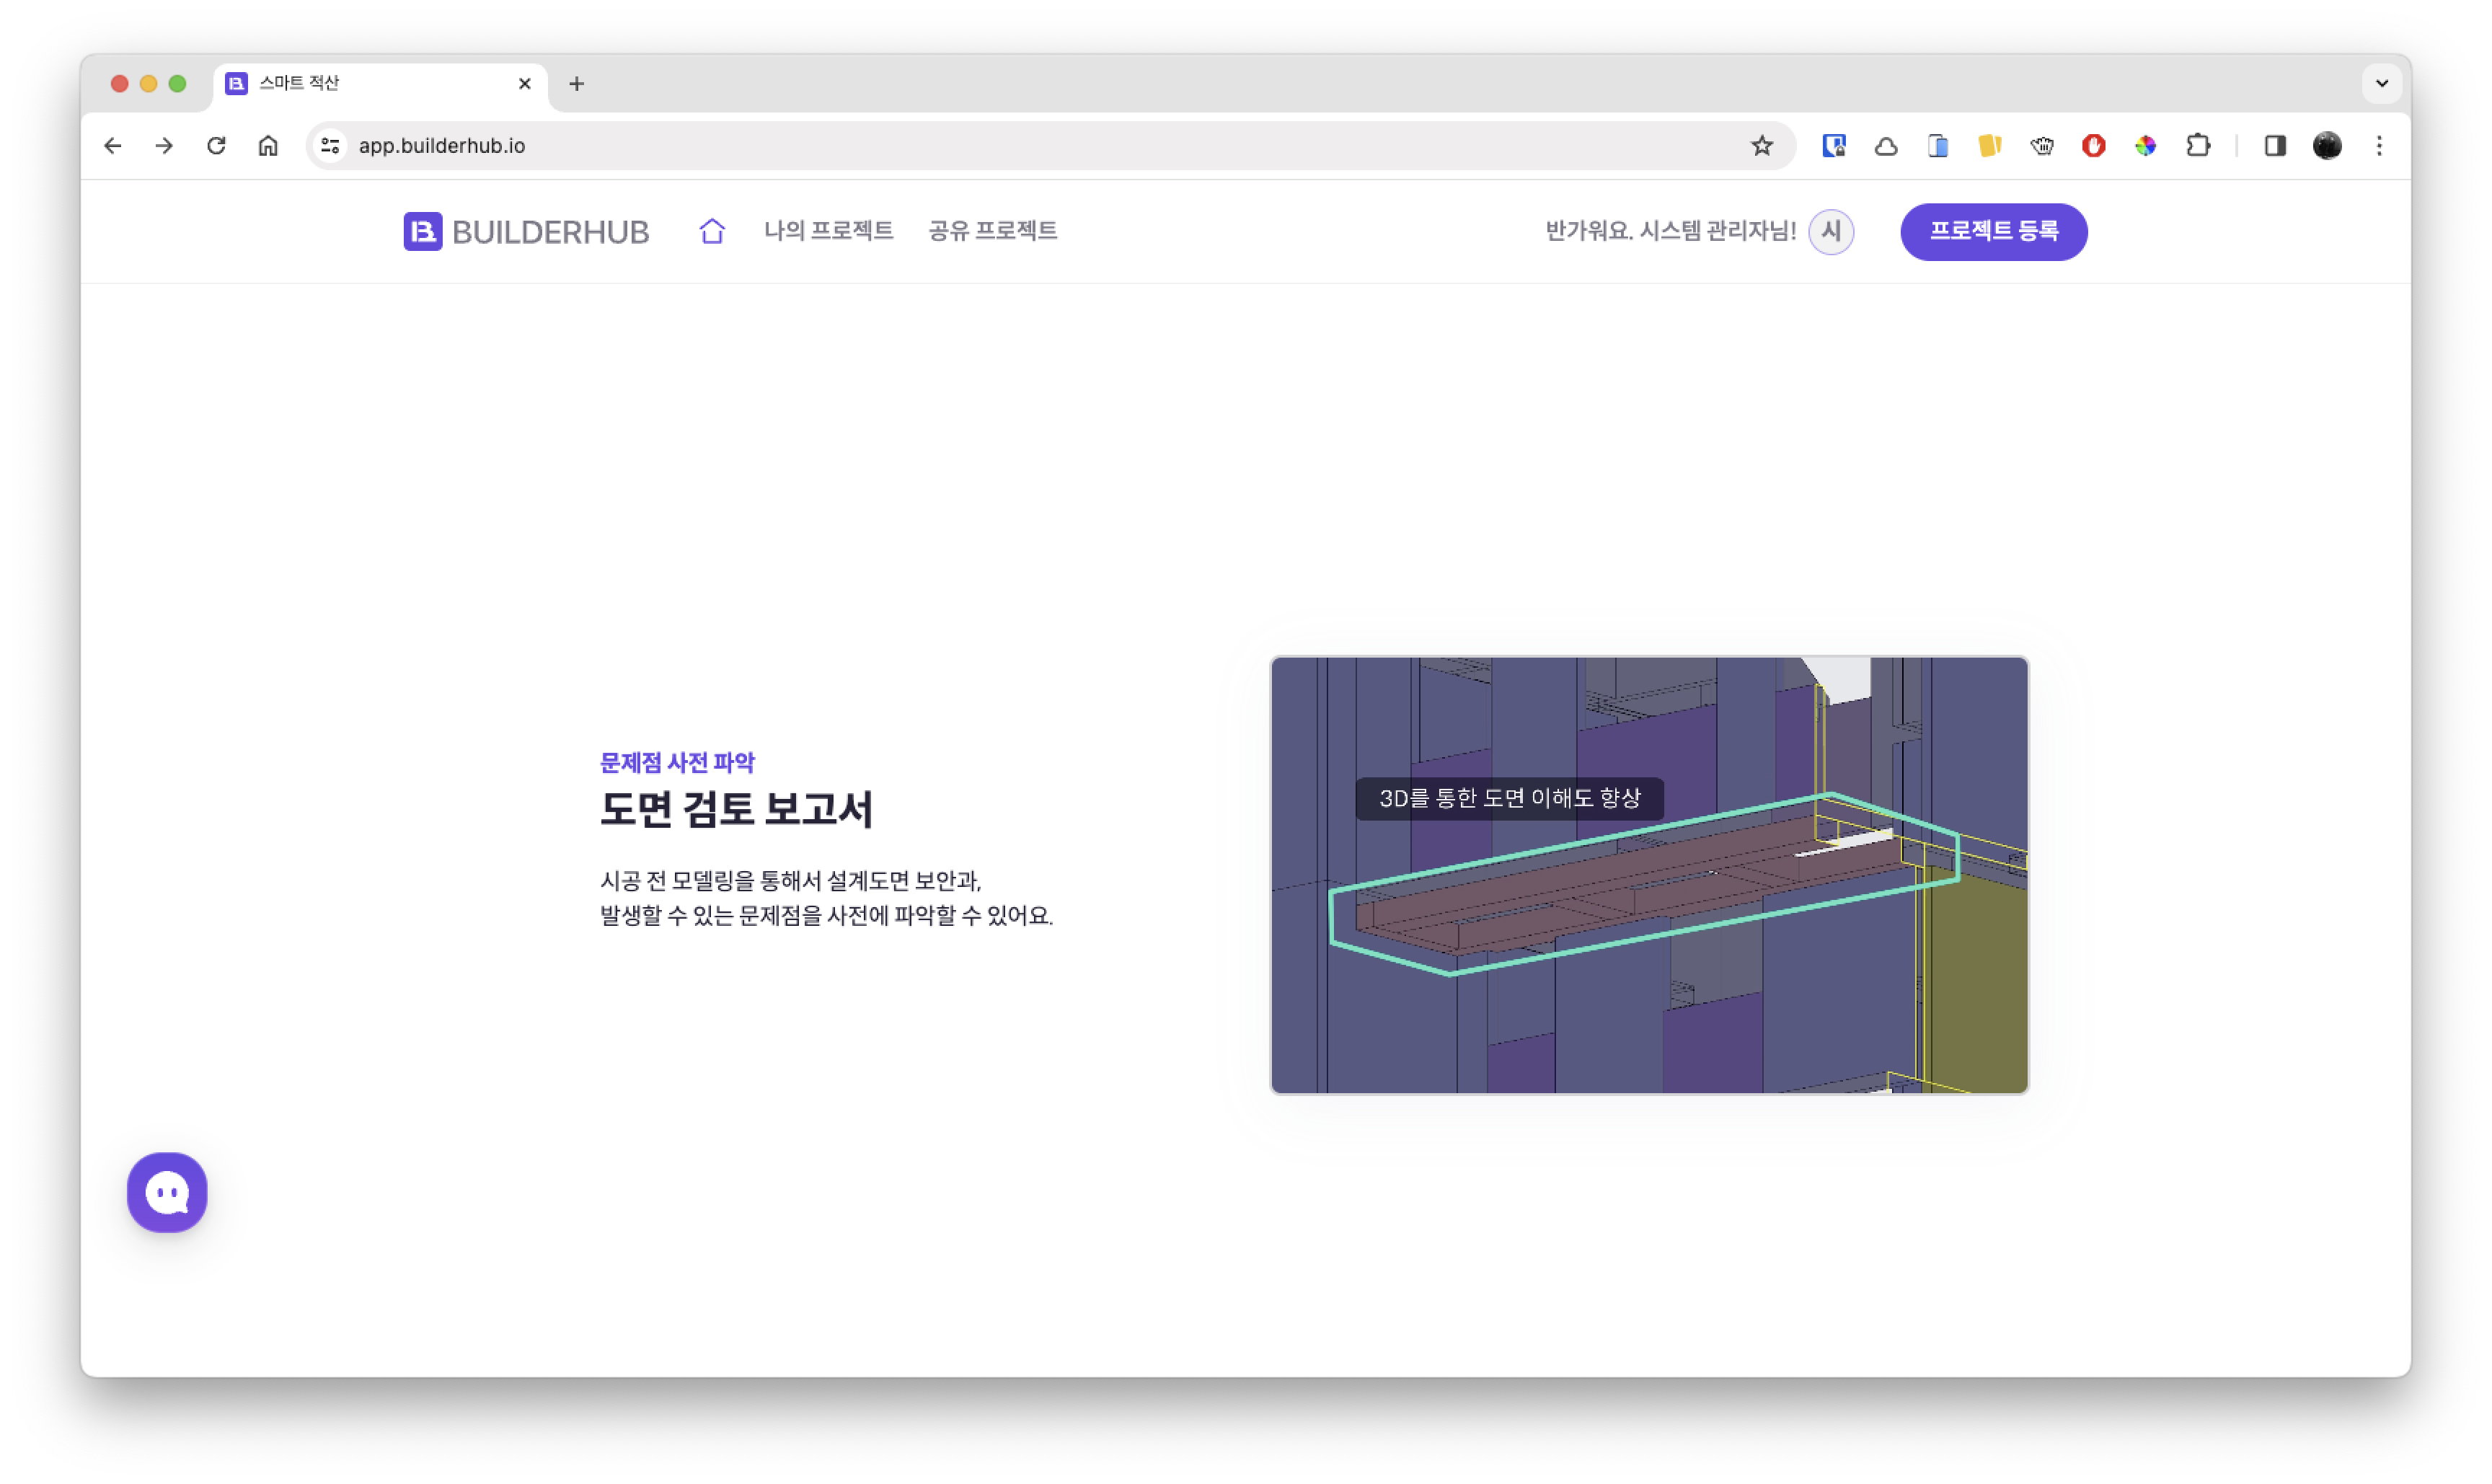
\includegraphics[width=0.35\textwidth]{images/builderhub-customer-4.png}
				      \caption*{Check drawing}
			      }
			      \parbox{0.35\textwidth}{
				      \centering
				      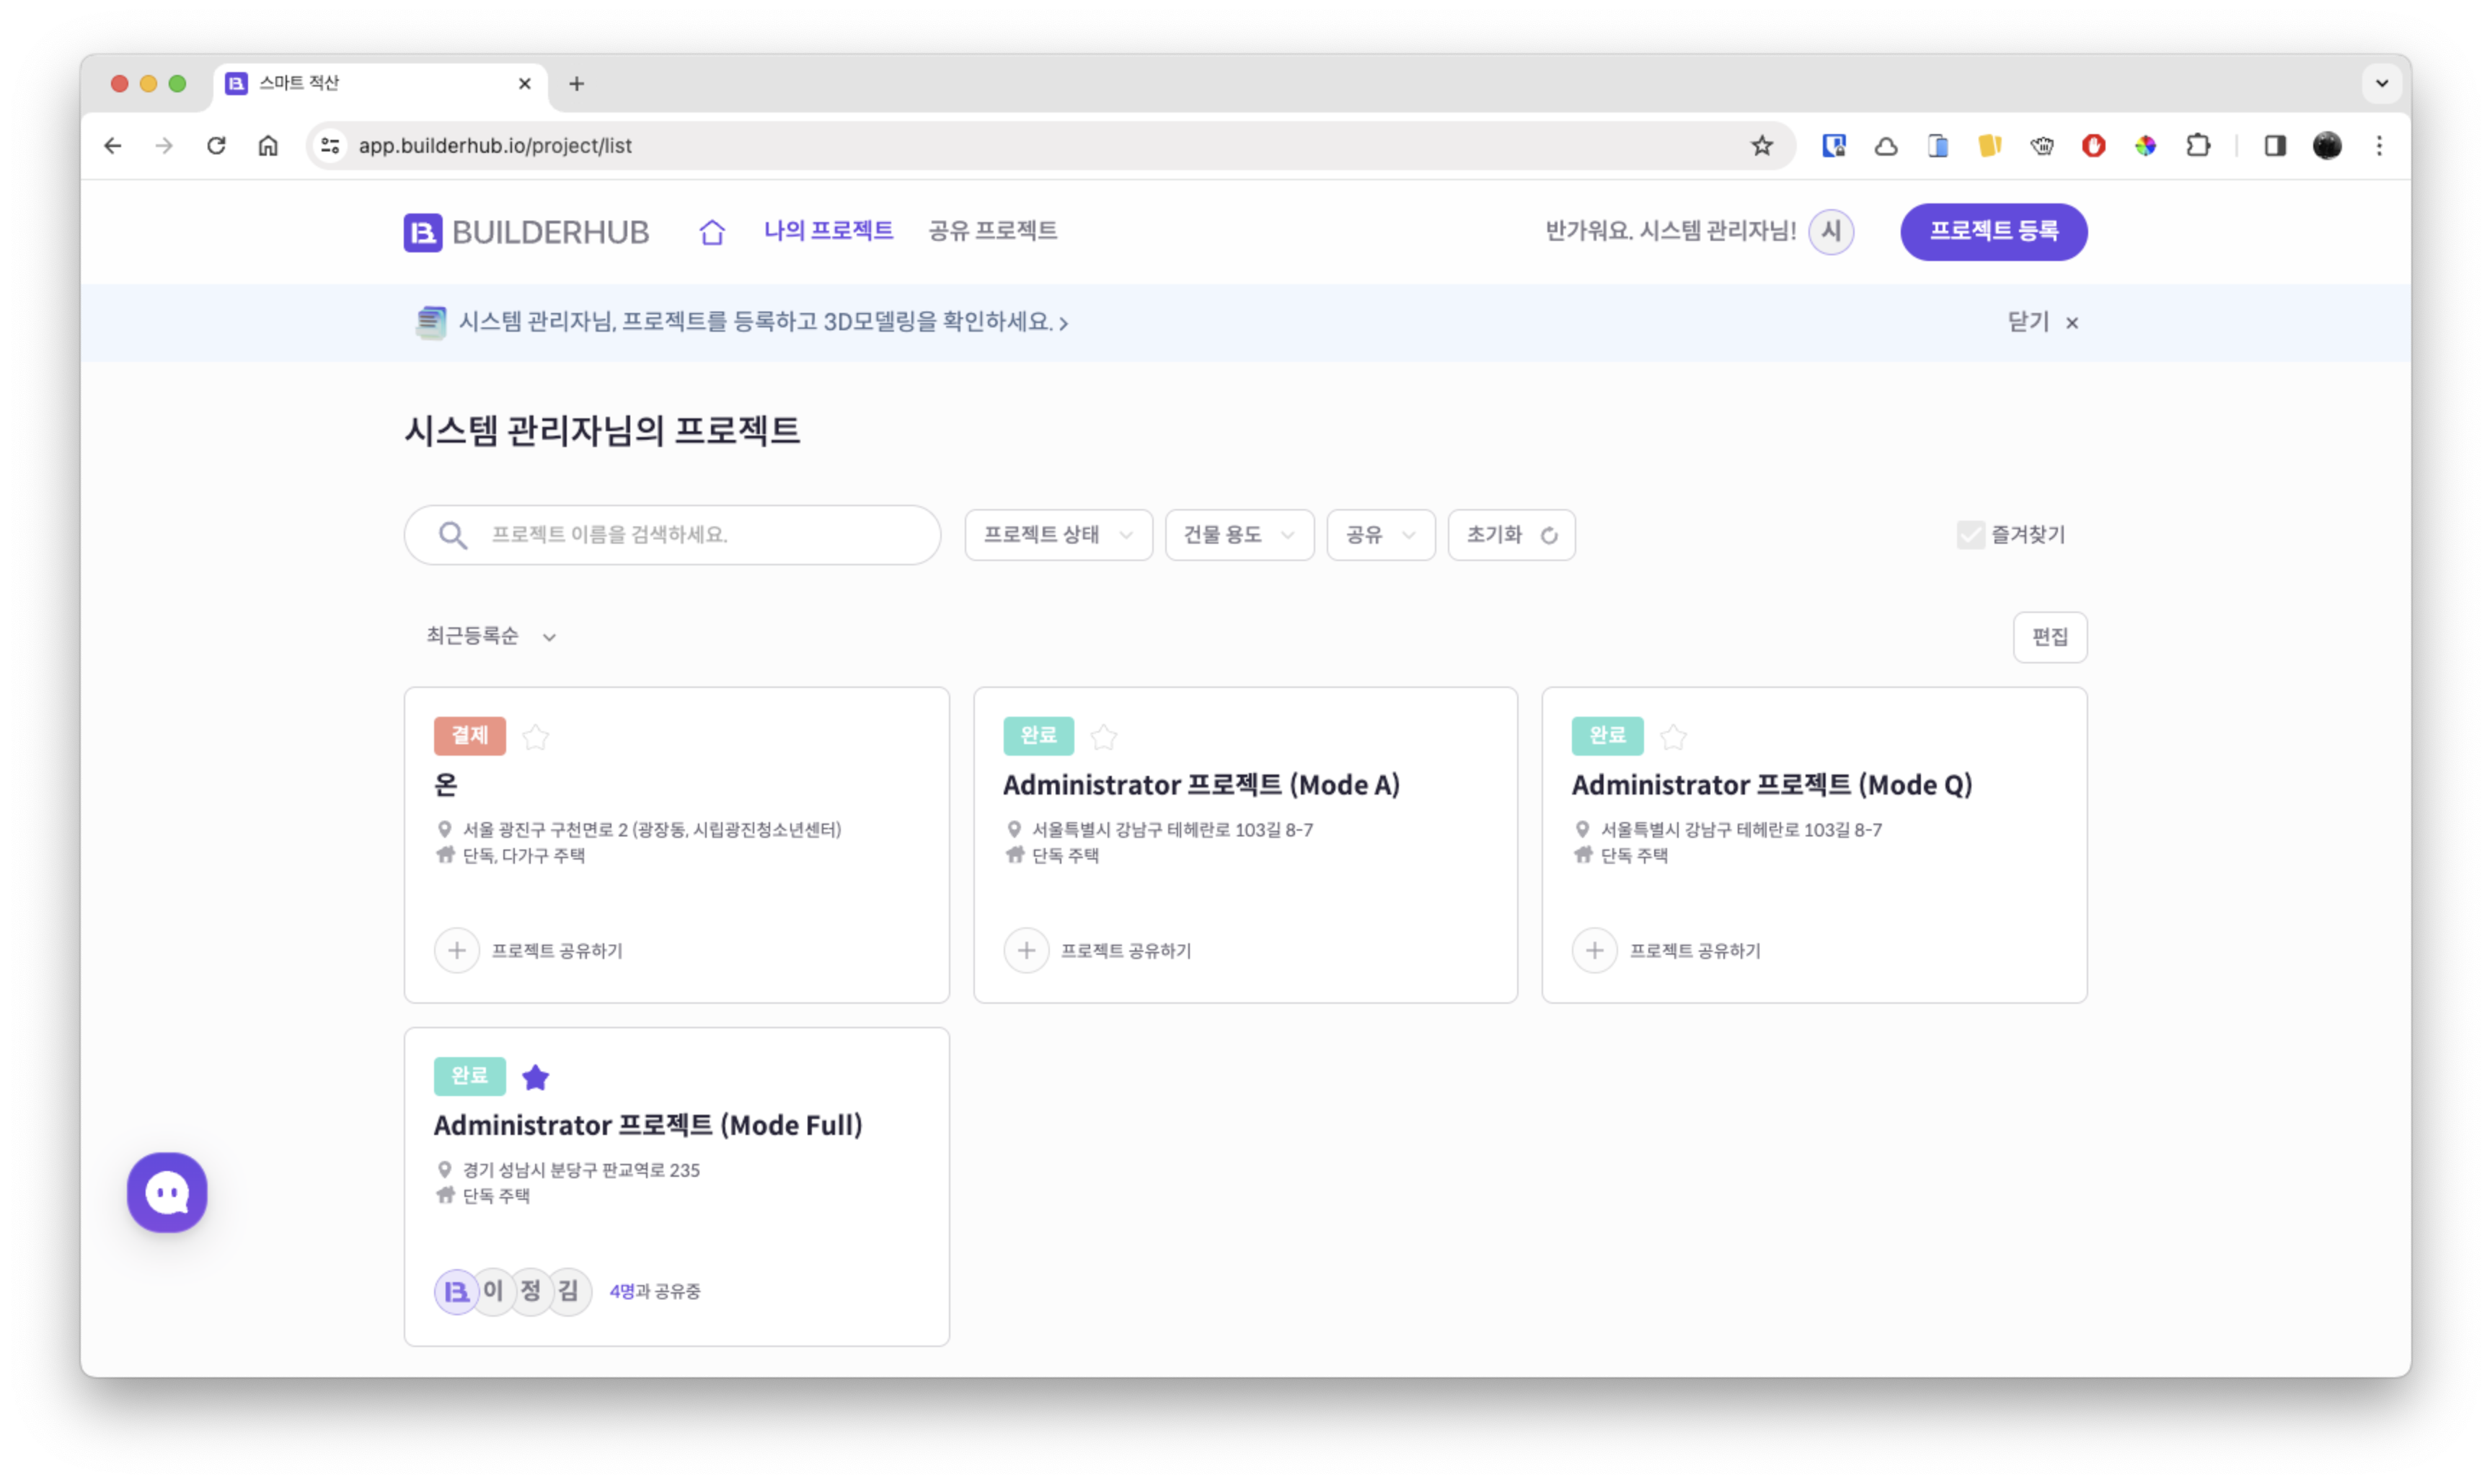
\includegraphics[width=0.35\textwidth]{images/builderhub-customer-project-1.png}
				      \caption*{Project list}
			      }\qquad
			      \parbox{0.35\textwidth}{
				      \centering
				      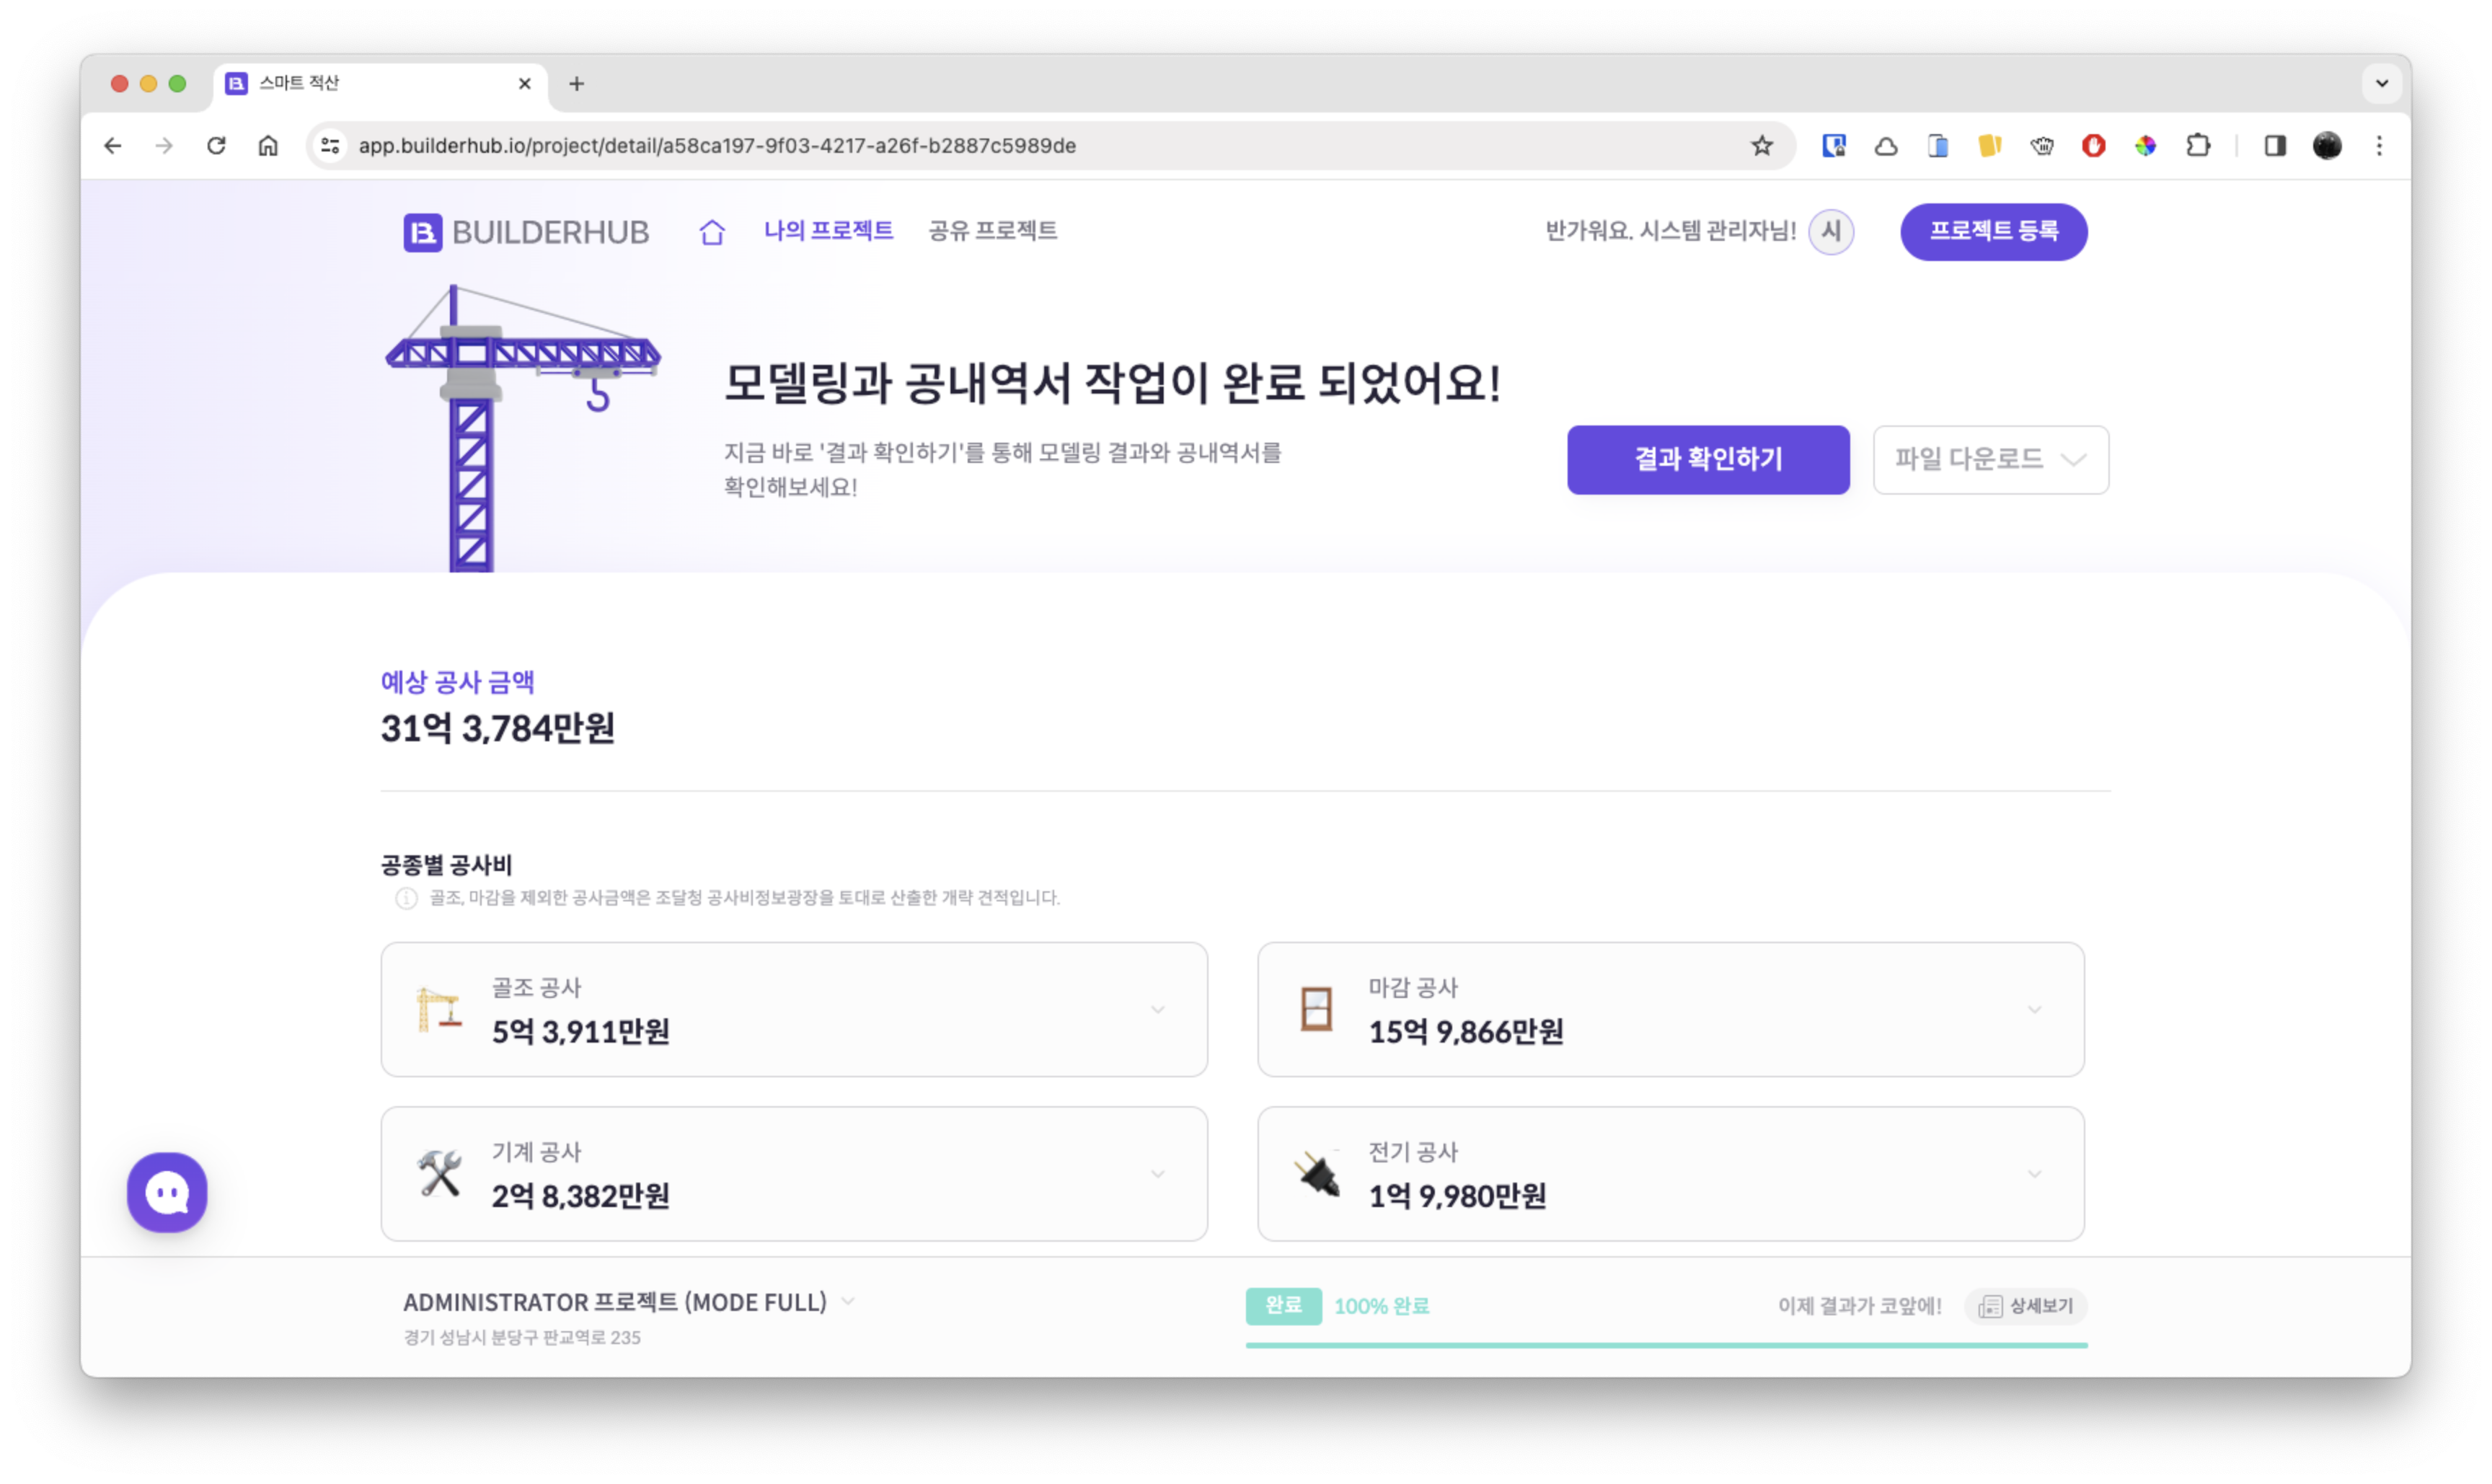
\includegraphics[width=0.35\textwidth]{images/builderhub-customer-project-2.png}
				      \caption*{Project completed}
			      }\qquad
			      \parbox{0.35\textwidth}{
				      \centering
				      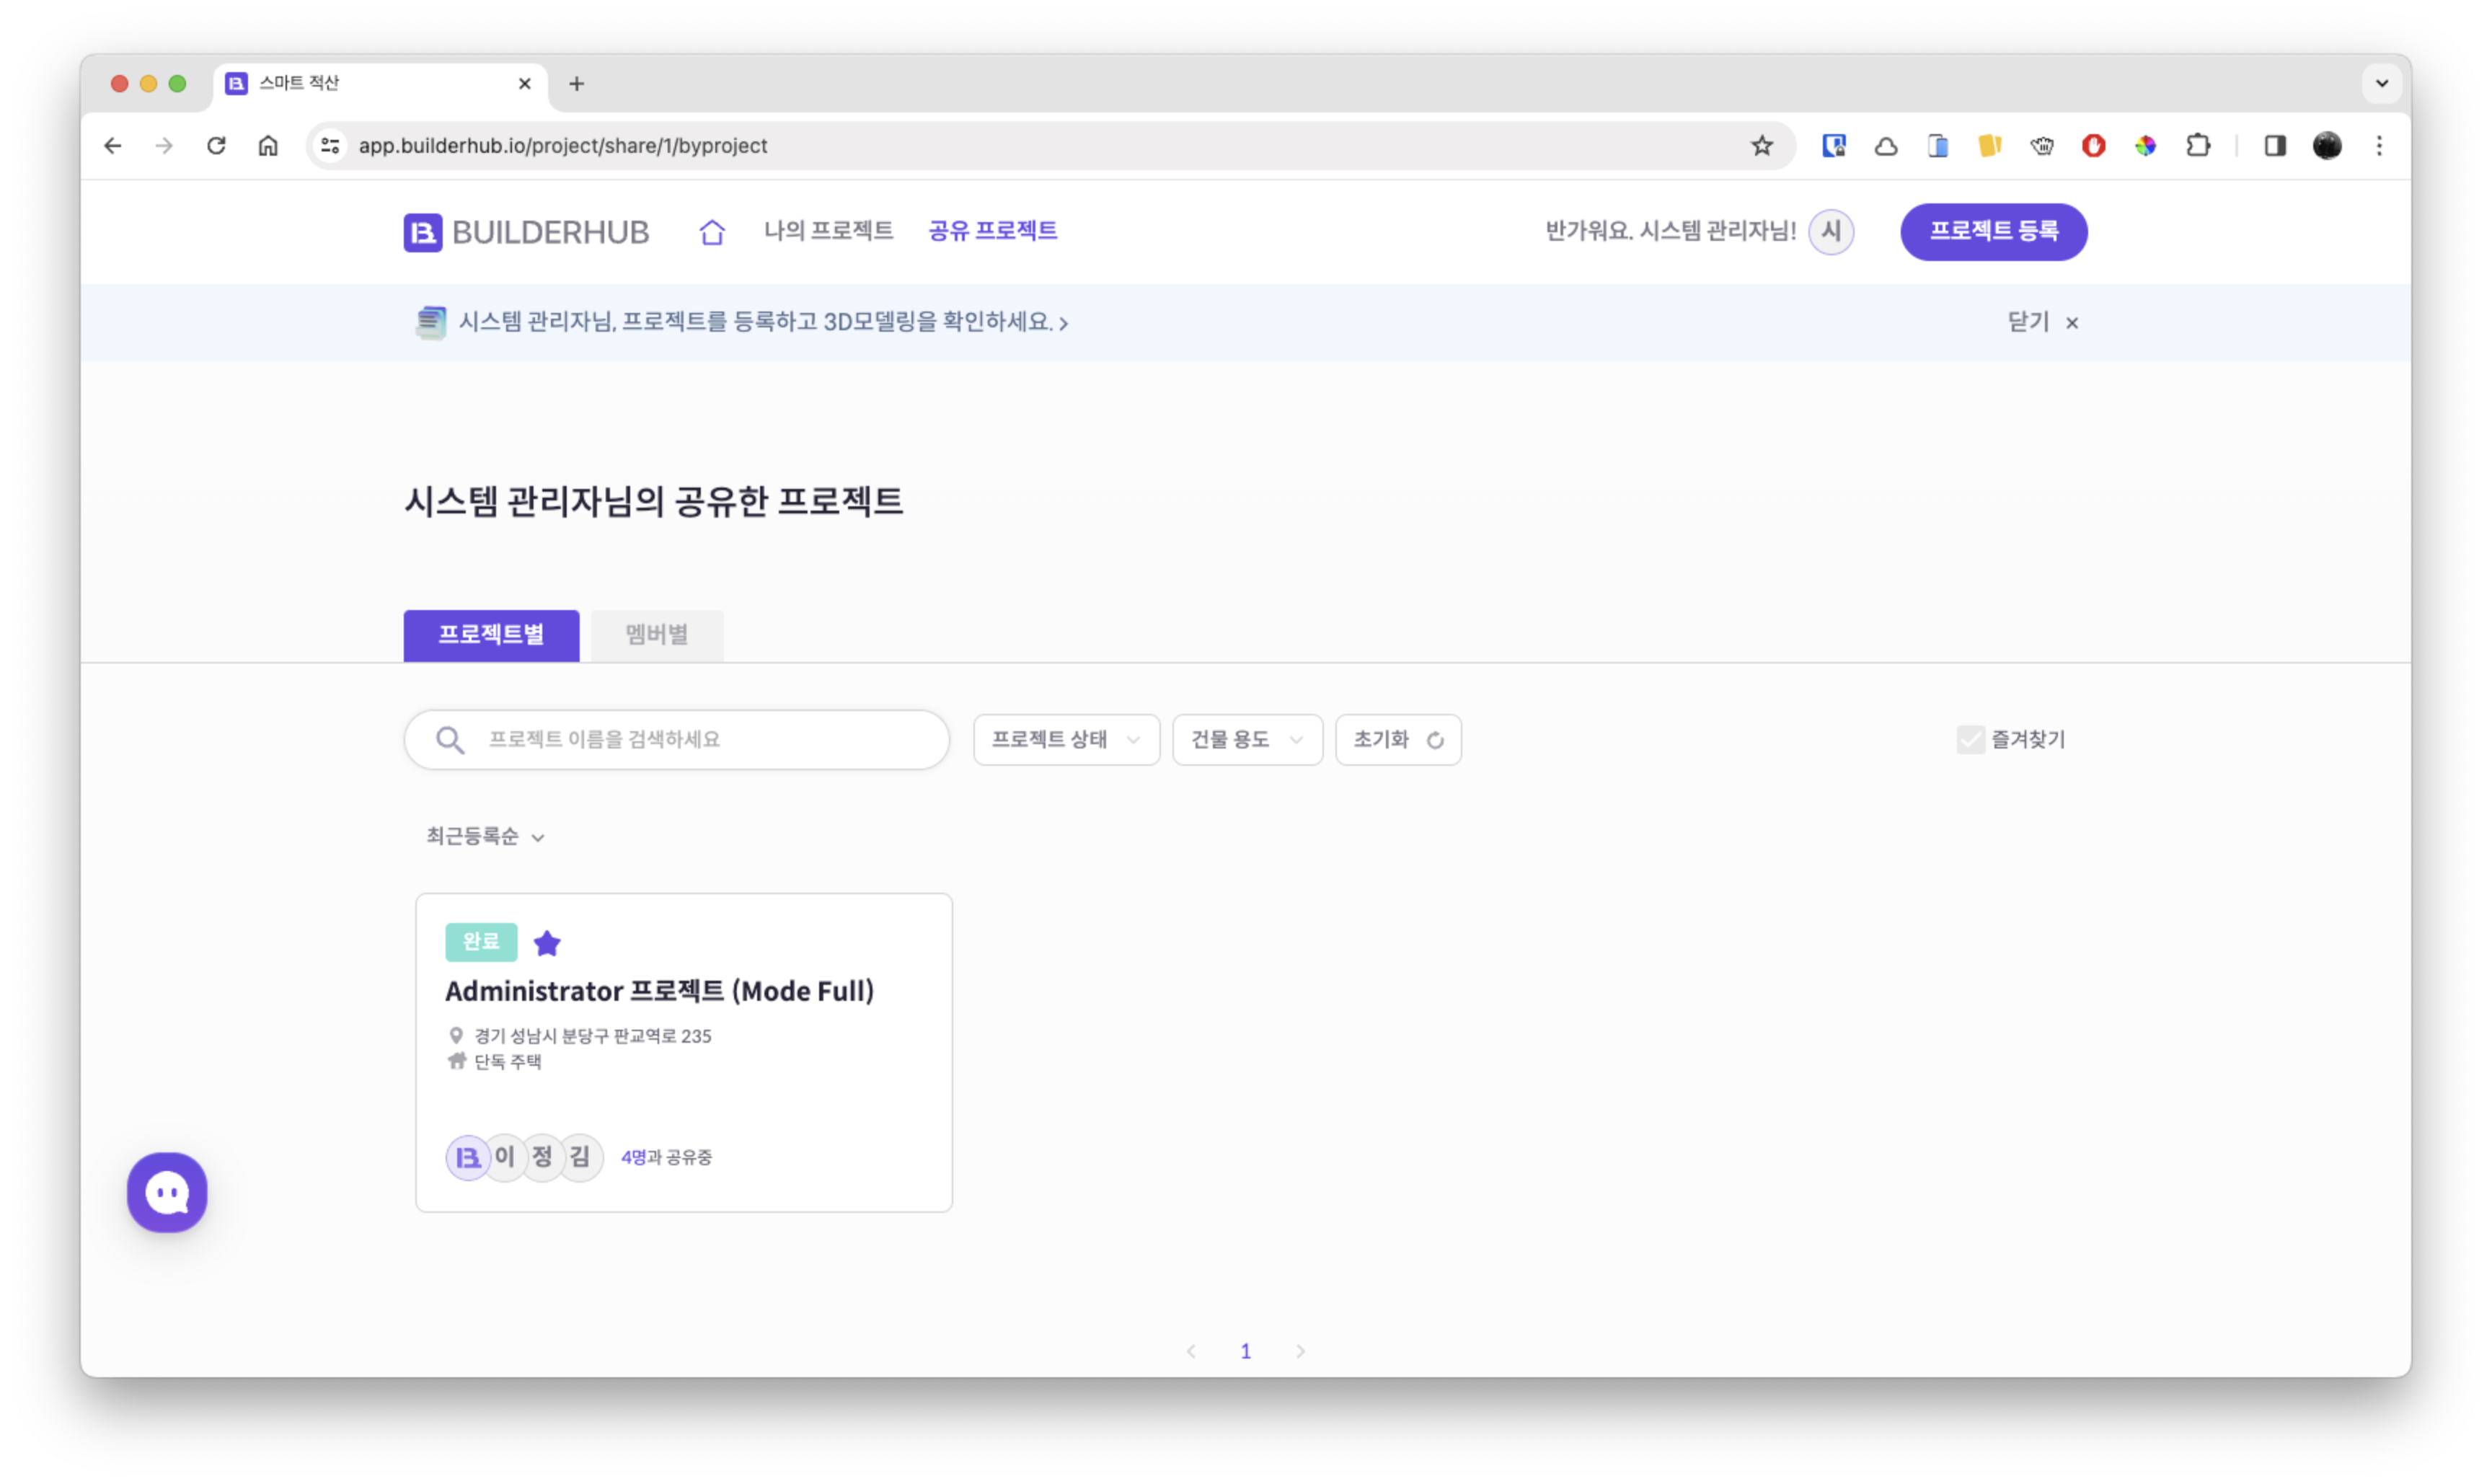
\includegraphics[width=0.35\textwidth]{images/builderhub-customer-project-3.png}
				      \caption*{Sharing project}
			      }\qquad
			      \parbox{0.35\textwidth}{
				      \centering
				      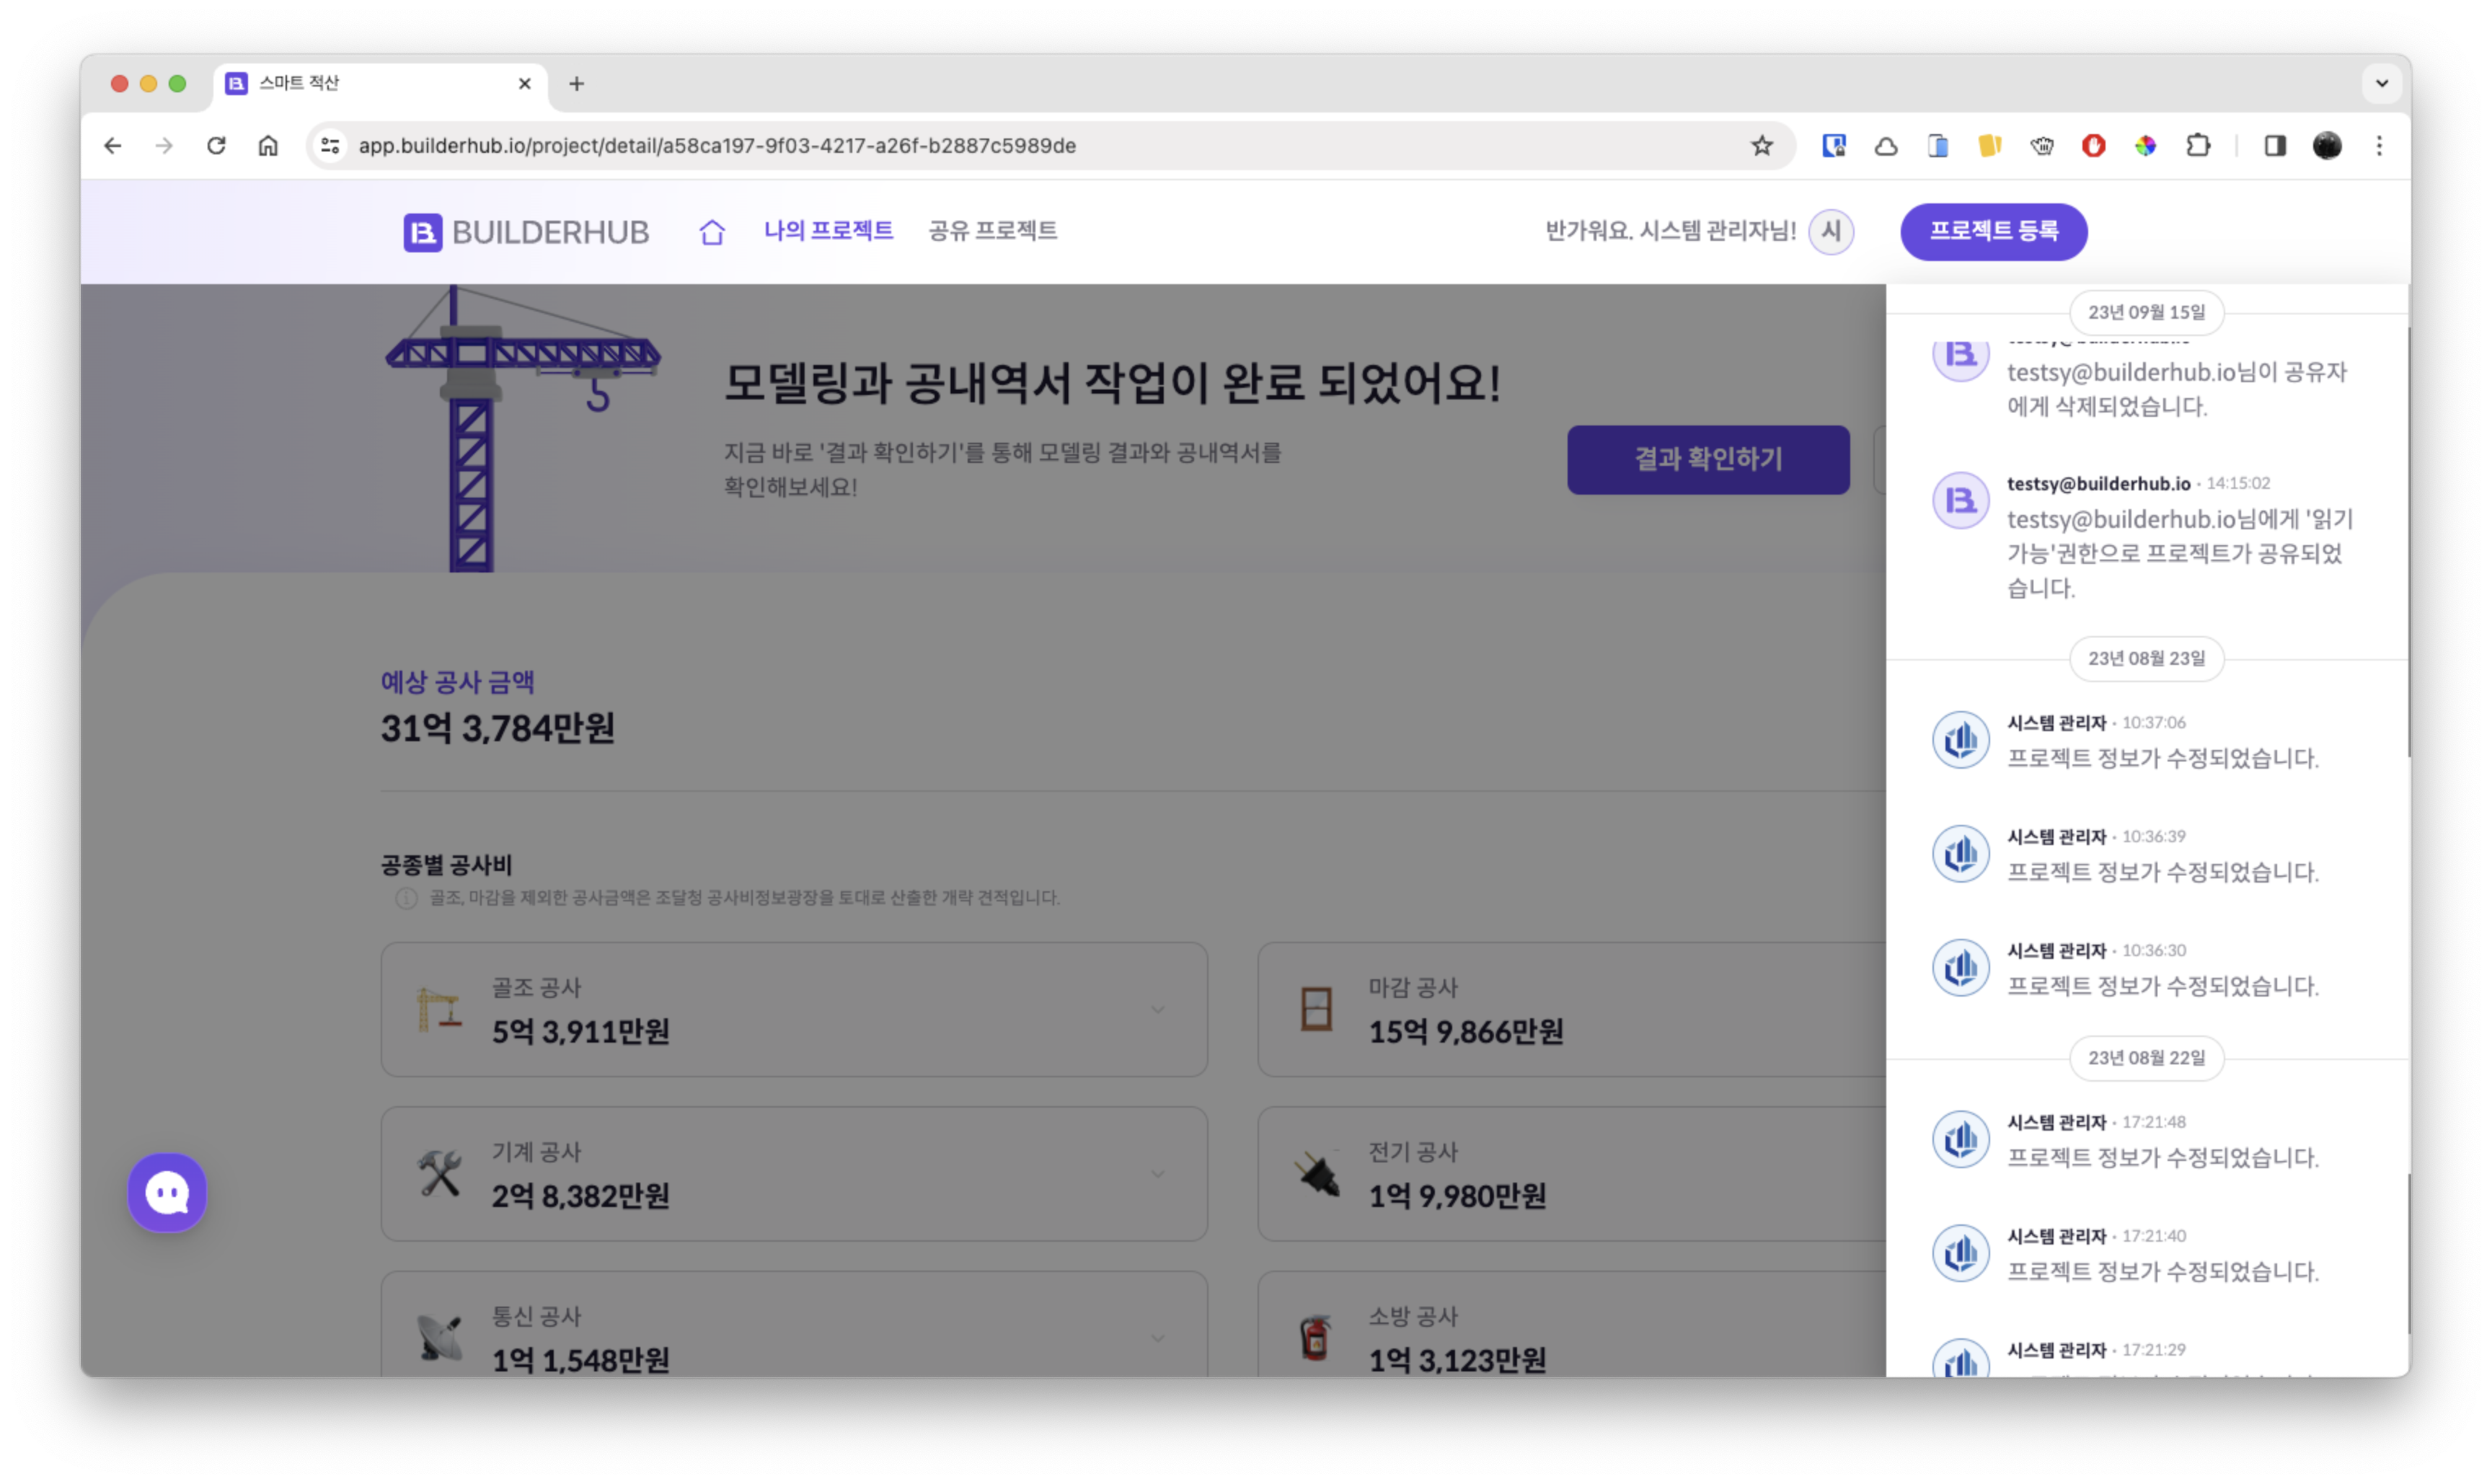
\includegraphics[width=0.35\textwidth]{images/builderhub-customer-project-4.png}
				      \caption*{Project history \& detail}
			      }
		      \end{fullwidth}
	      \end{figure}
	      \clearpage
	\item \href{https://curation.builderhub.io/project/tester}{큐레이션 서비스} 개발
	      \begin{itemize}
		      \item BIM 모델 3D 뷰어: Three.js, Forge API, Zoom to Control, First-person View Control
		      \item 내역 필터 및 검색: Floor Filter, Material Filter, Table Filter, Search
		      \item 모델 툴 개발: Section View, Screenshot, Measurement
		      \item 자재 변경, 도면 뷰어
		      \item 공정 시뮬레이션, 공정표 제공: Gantt Chart, Work simulation (on developing)
	      \end{itemize}
	      \begin{figure}[!ht]
		      \begin{fullwidth}
			      \parbox{0.35\textwidth}{
				      \centering
				      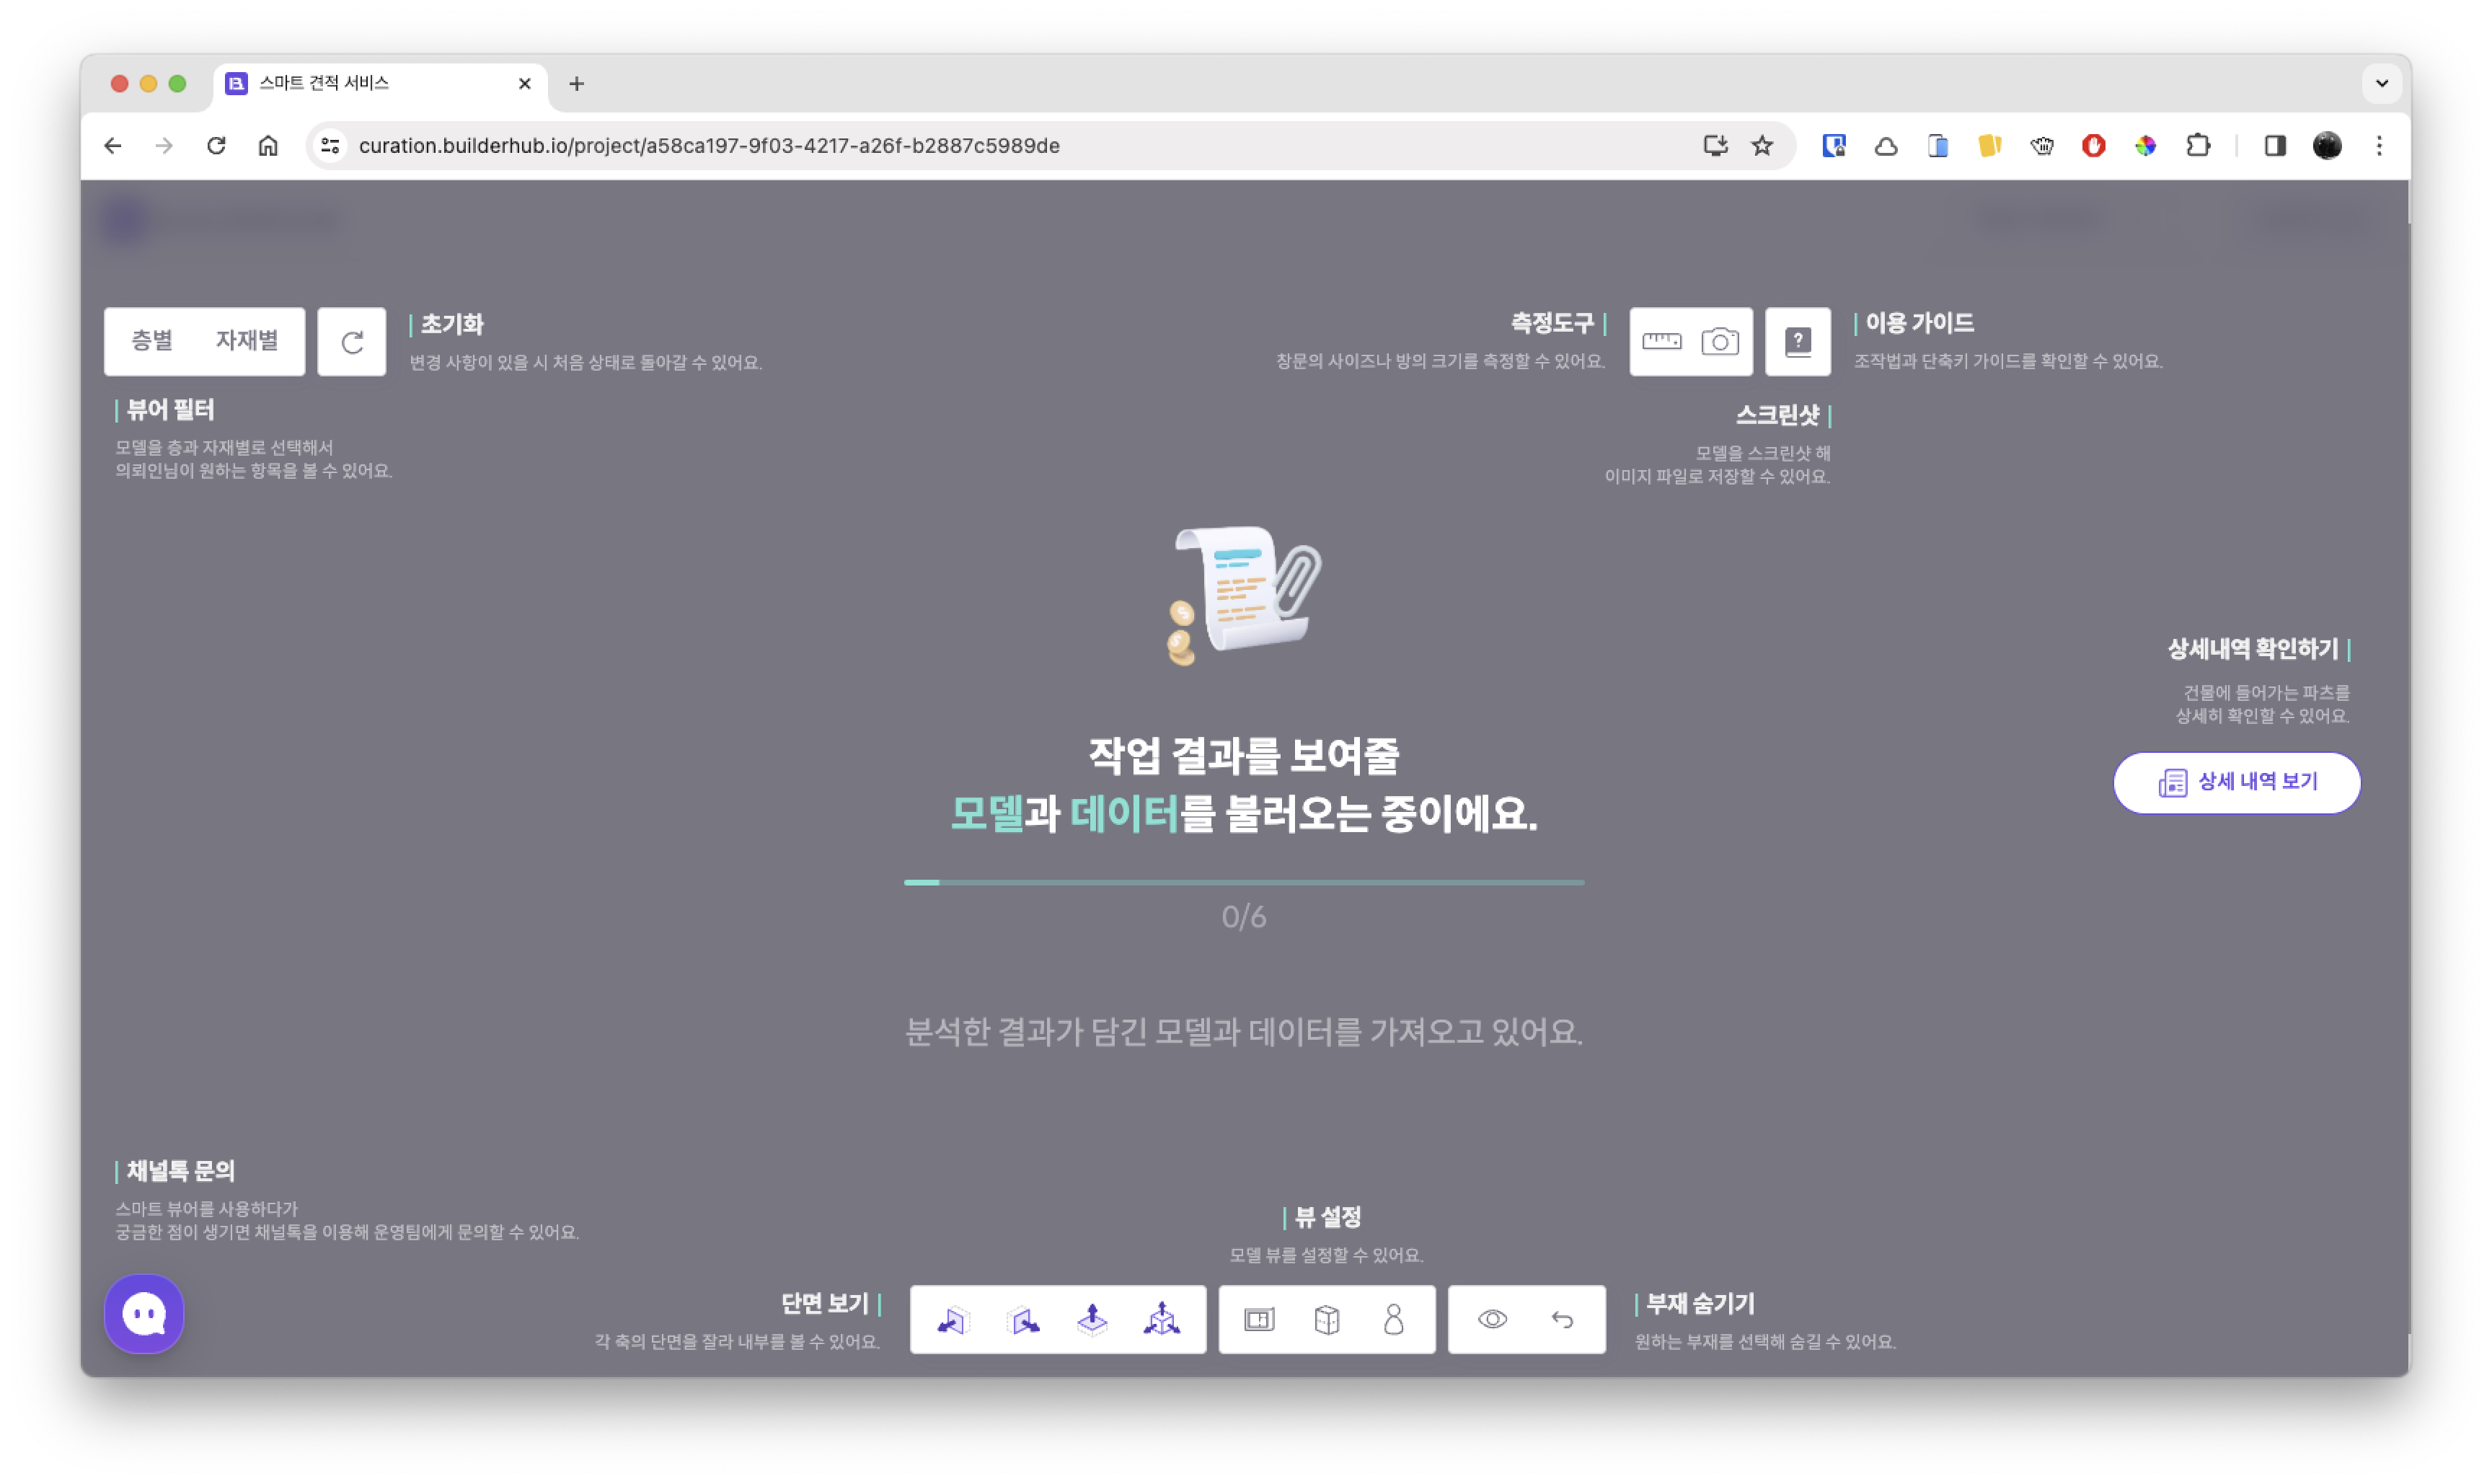
\includegraphics[width=0.35\textwidth]{images/builderhub-curation-loader-1.png}
				      \caption*{Loader}
			      }\qquad
			      \parbox{0.35\textwidth}{
				      \centering
				      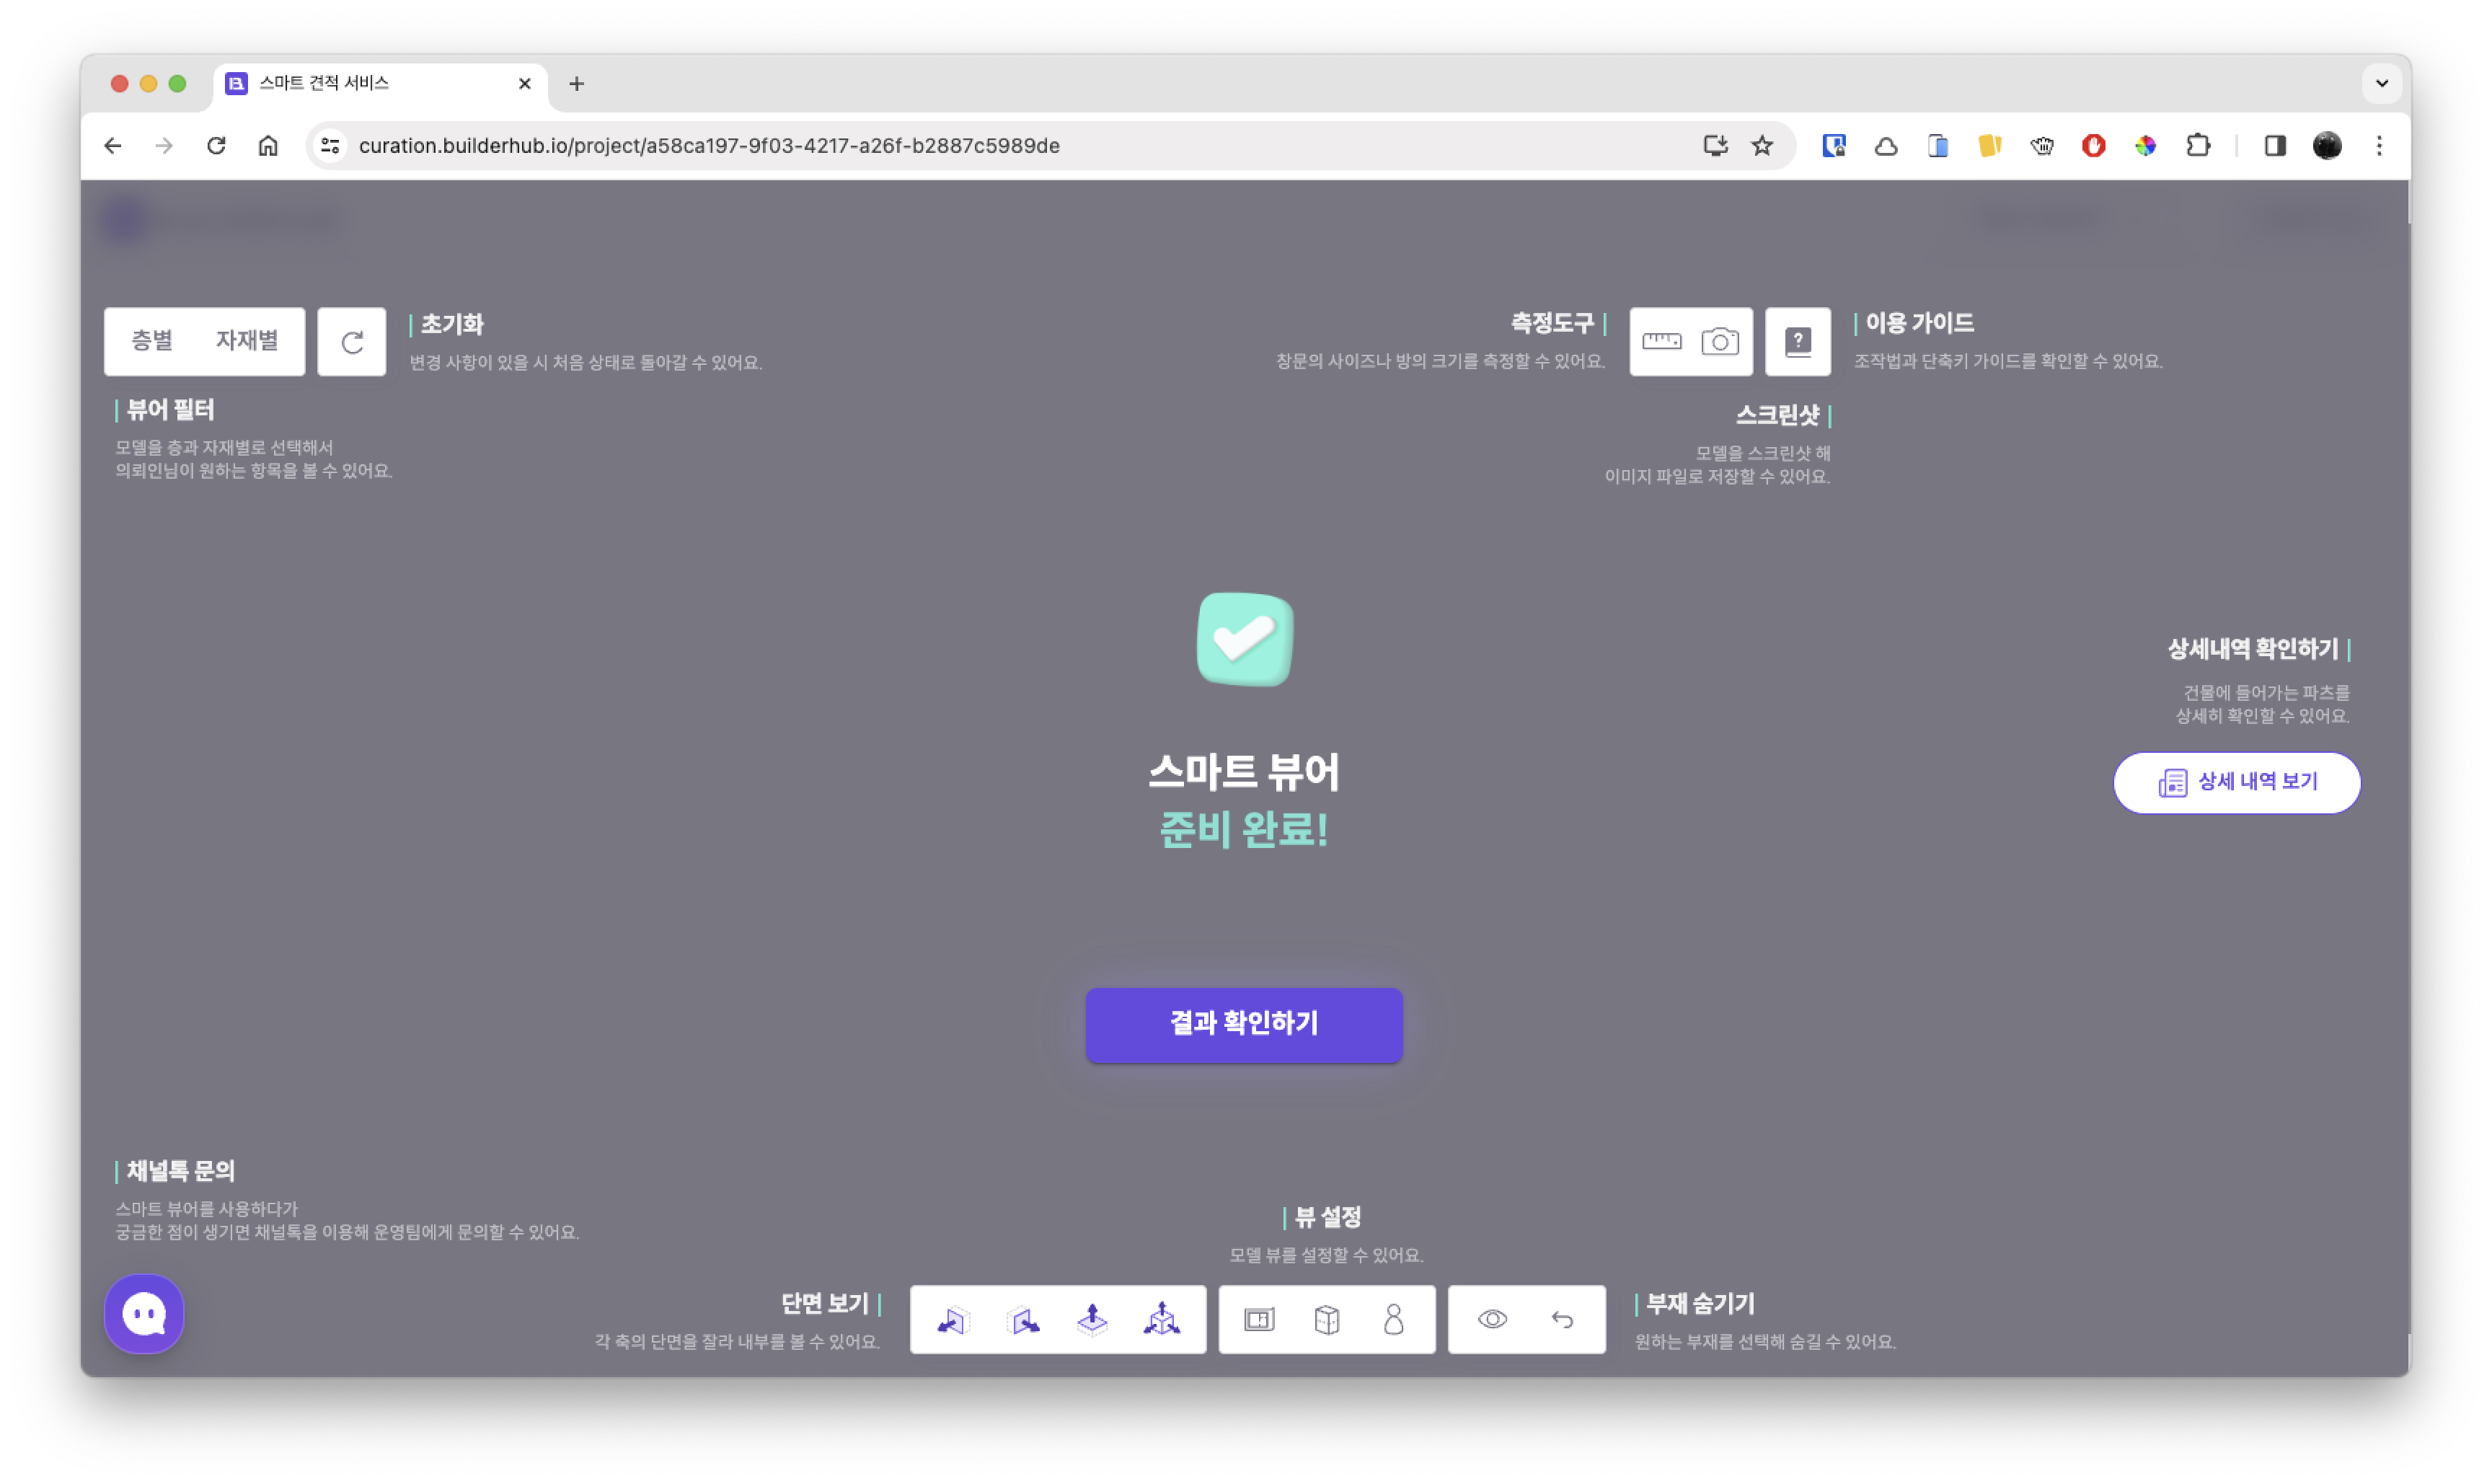
\includegraphics[width=0.35\textwidth]{images/builderhub-curation-loader-2.png}
				      \caption*{Loading done}
			      }\qquad
			      \parbox{0.35\textwidth}{
				      \centering
				      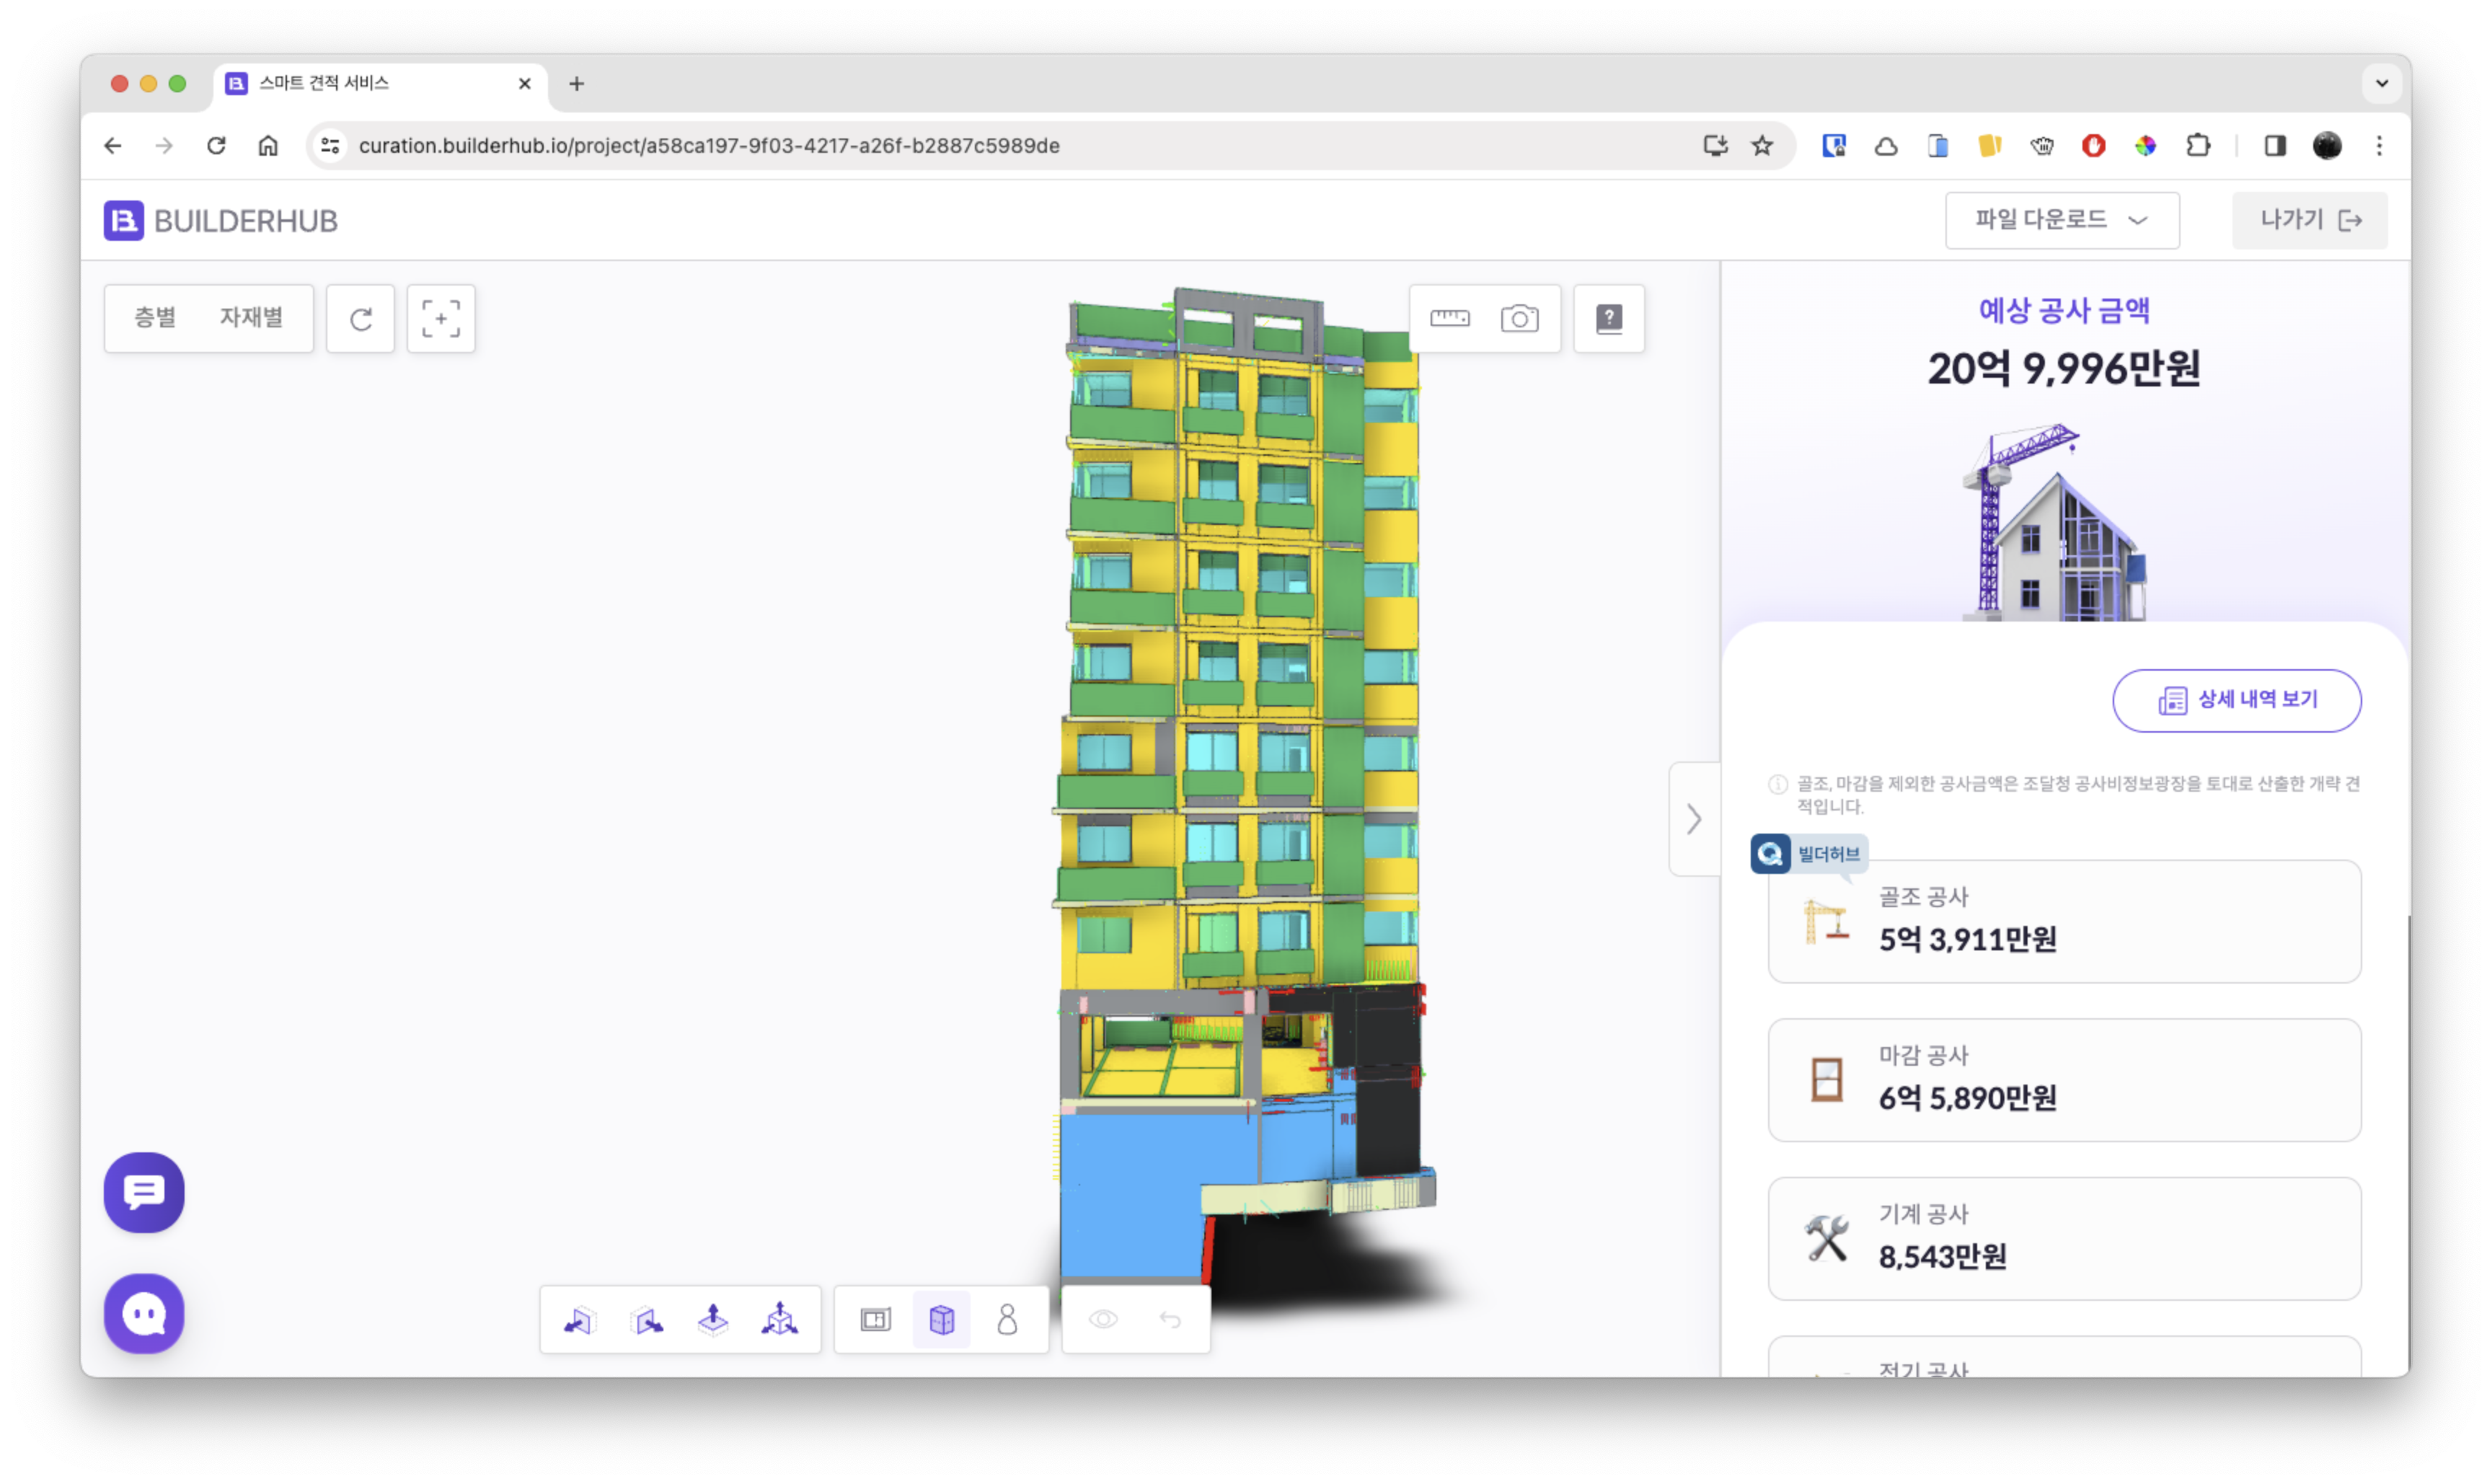
\includegraphics[width=0.35\textwidth]{images/builderhub-curation-main.png}
				      \caption*{Main view}
			      }\qquad
			      \parbox{0.35\textwidth}{
				      \centering
				      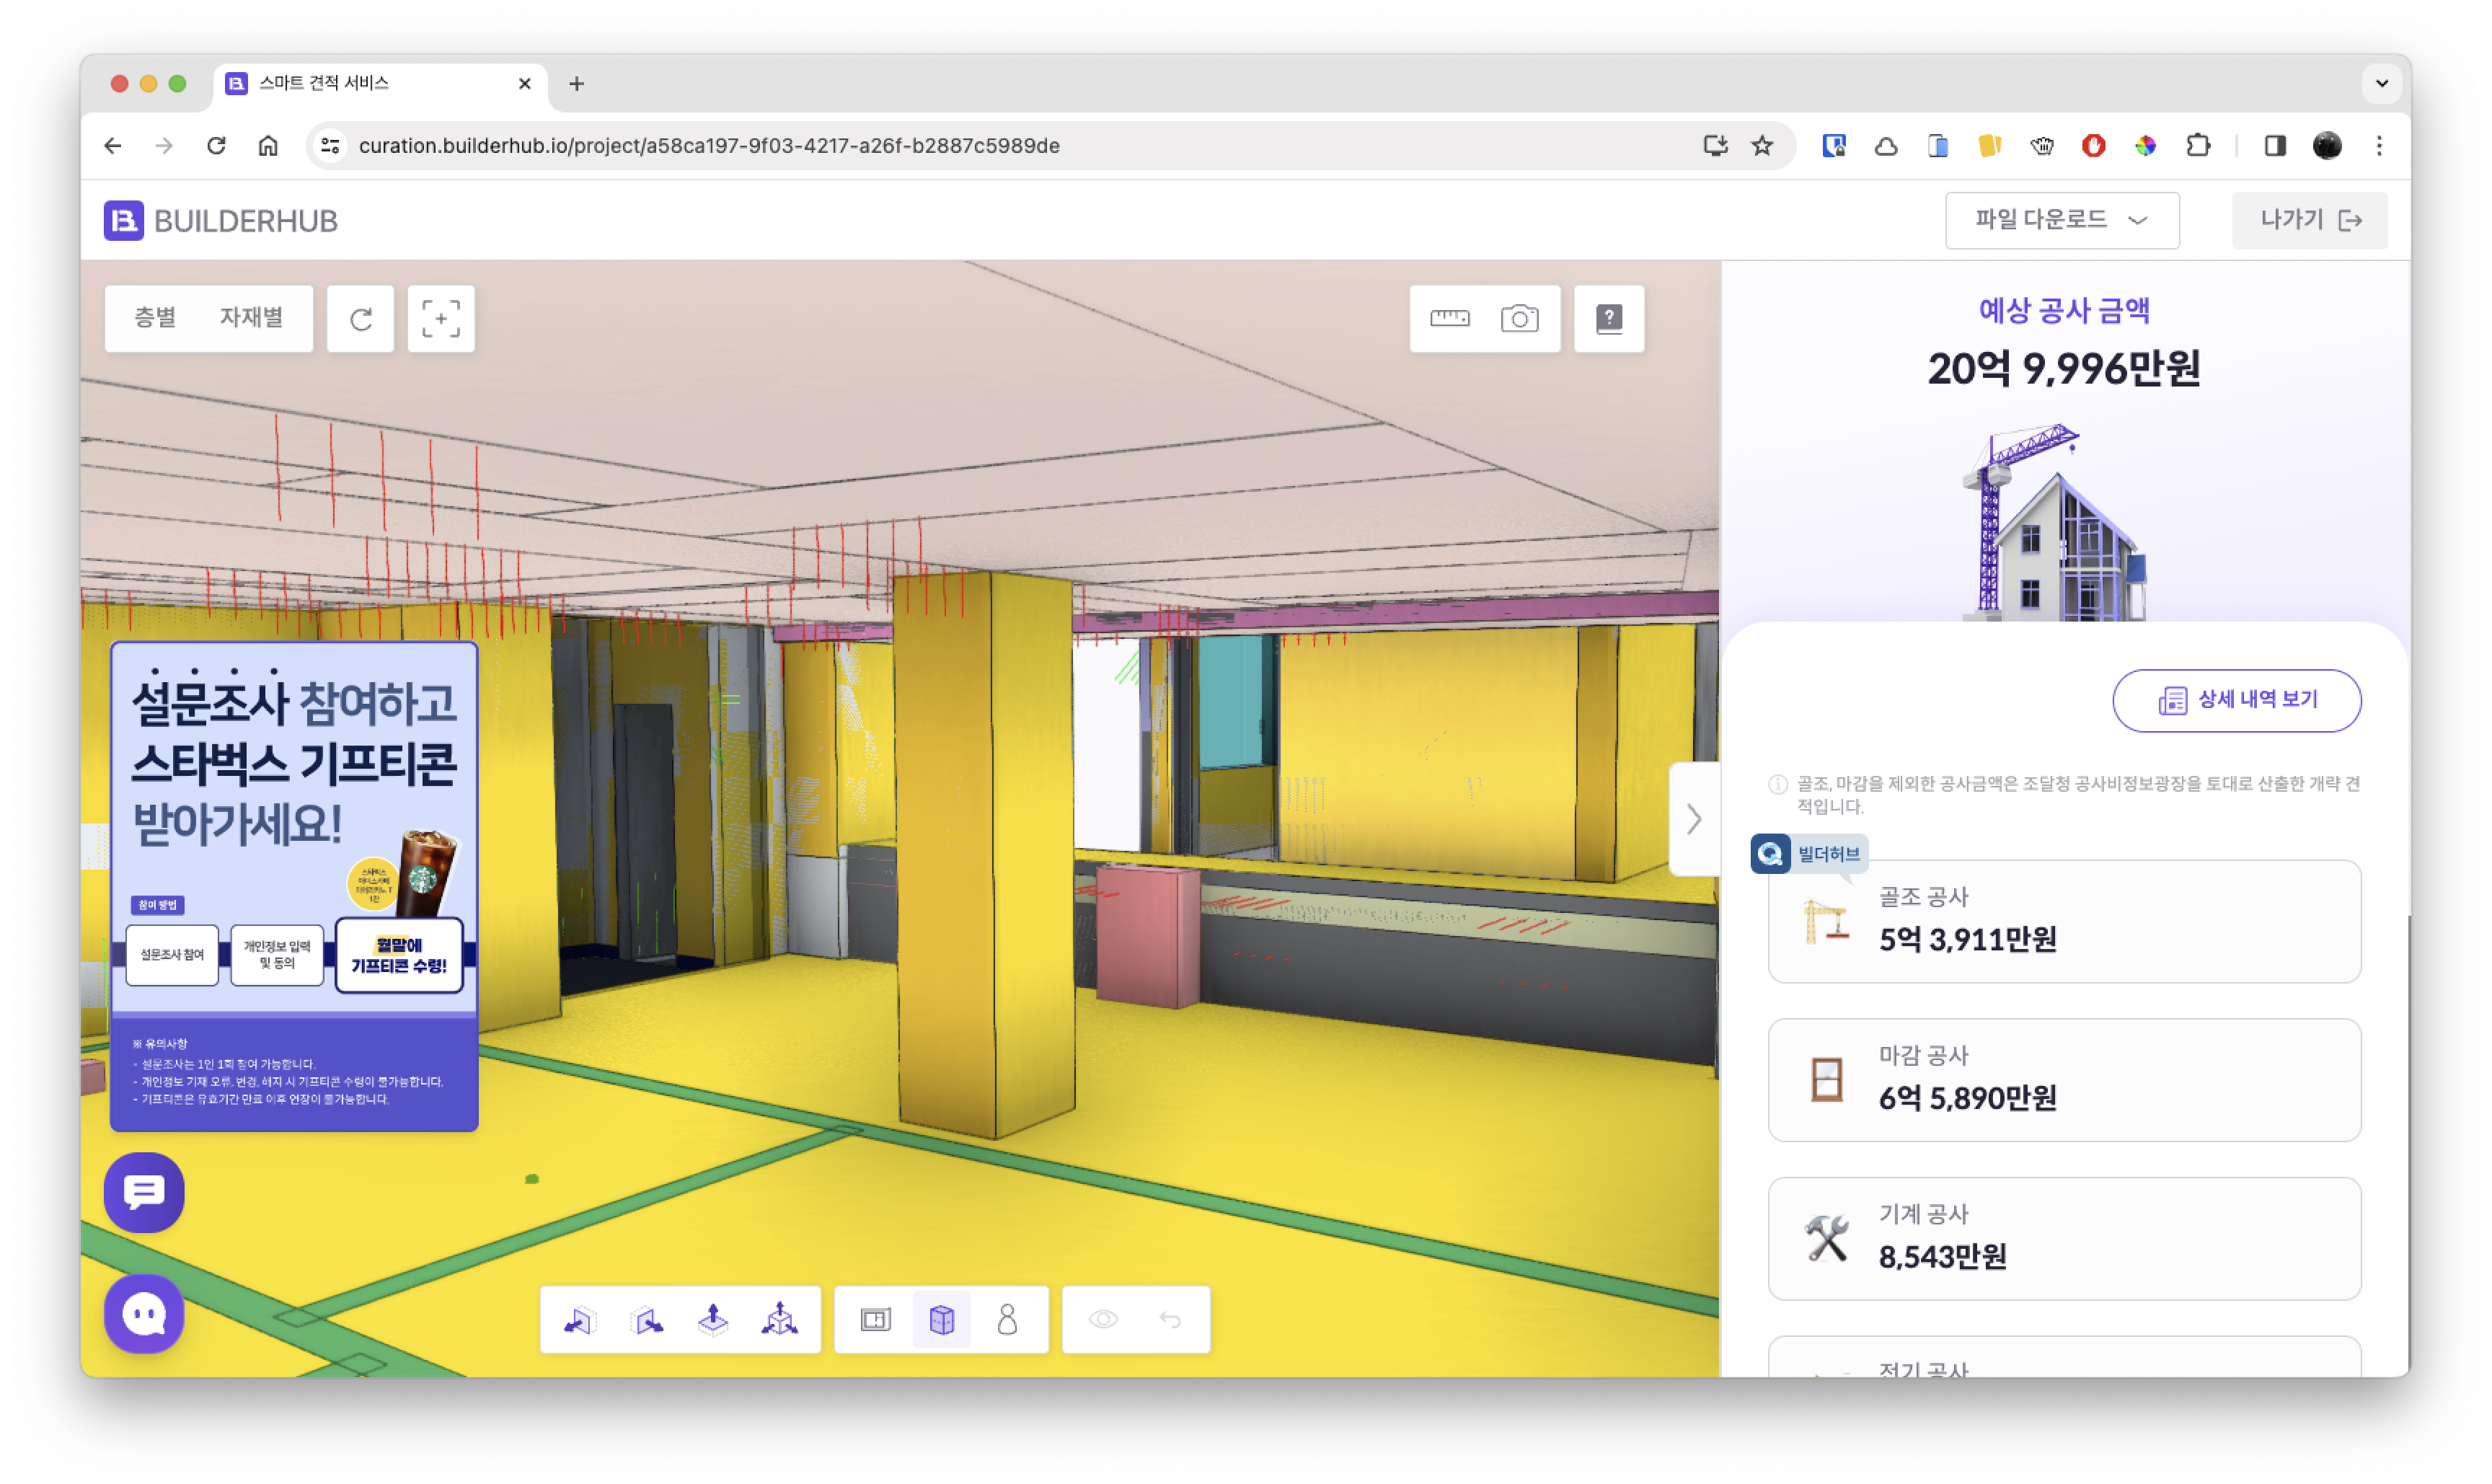
\includegraphics[width=0.35\textwidth]{images/builderhub-curation-control.png}
				      \caption*{Control orbit}
			      }
			      \parbox{0.35\textwidth}{
				      \centering
				      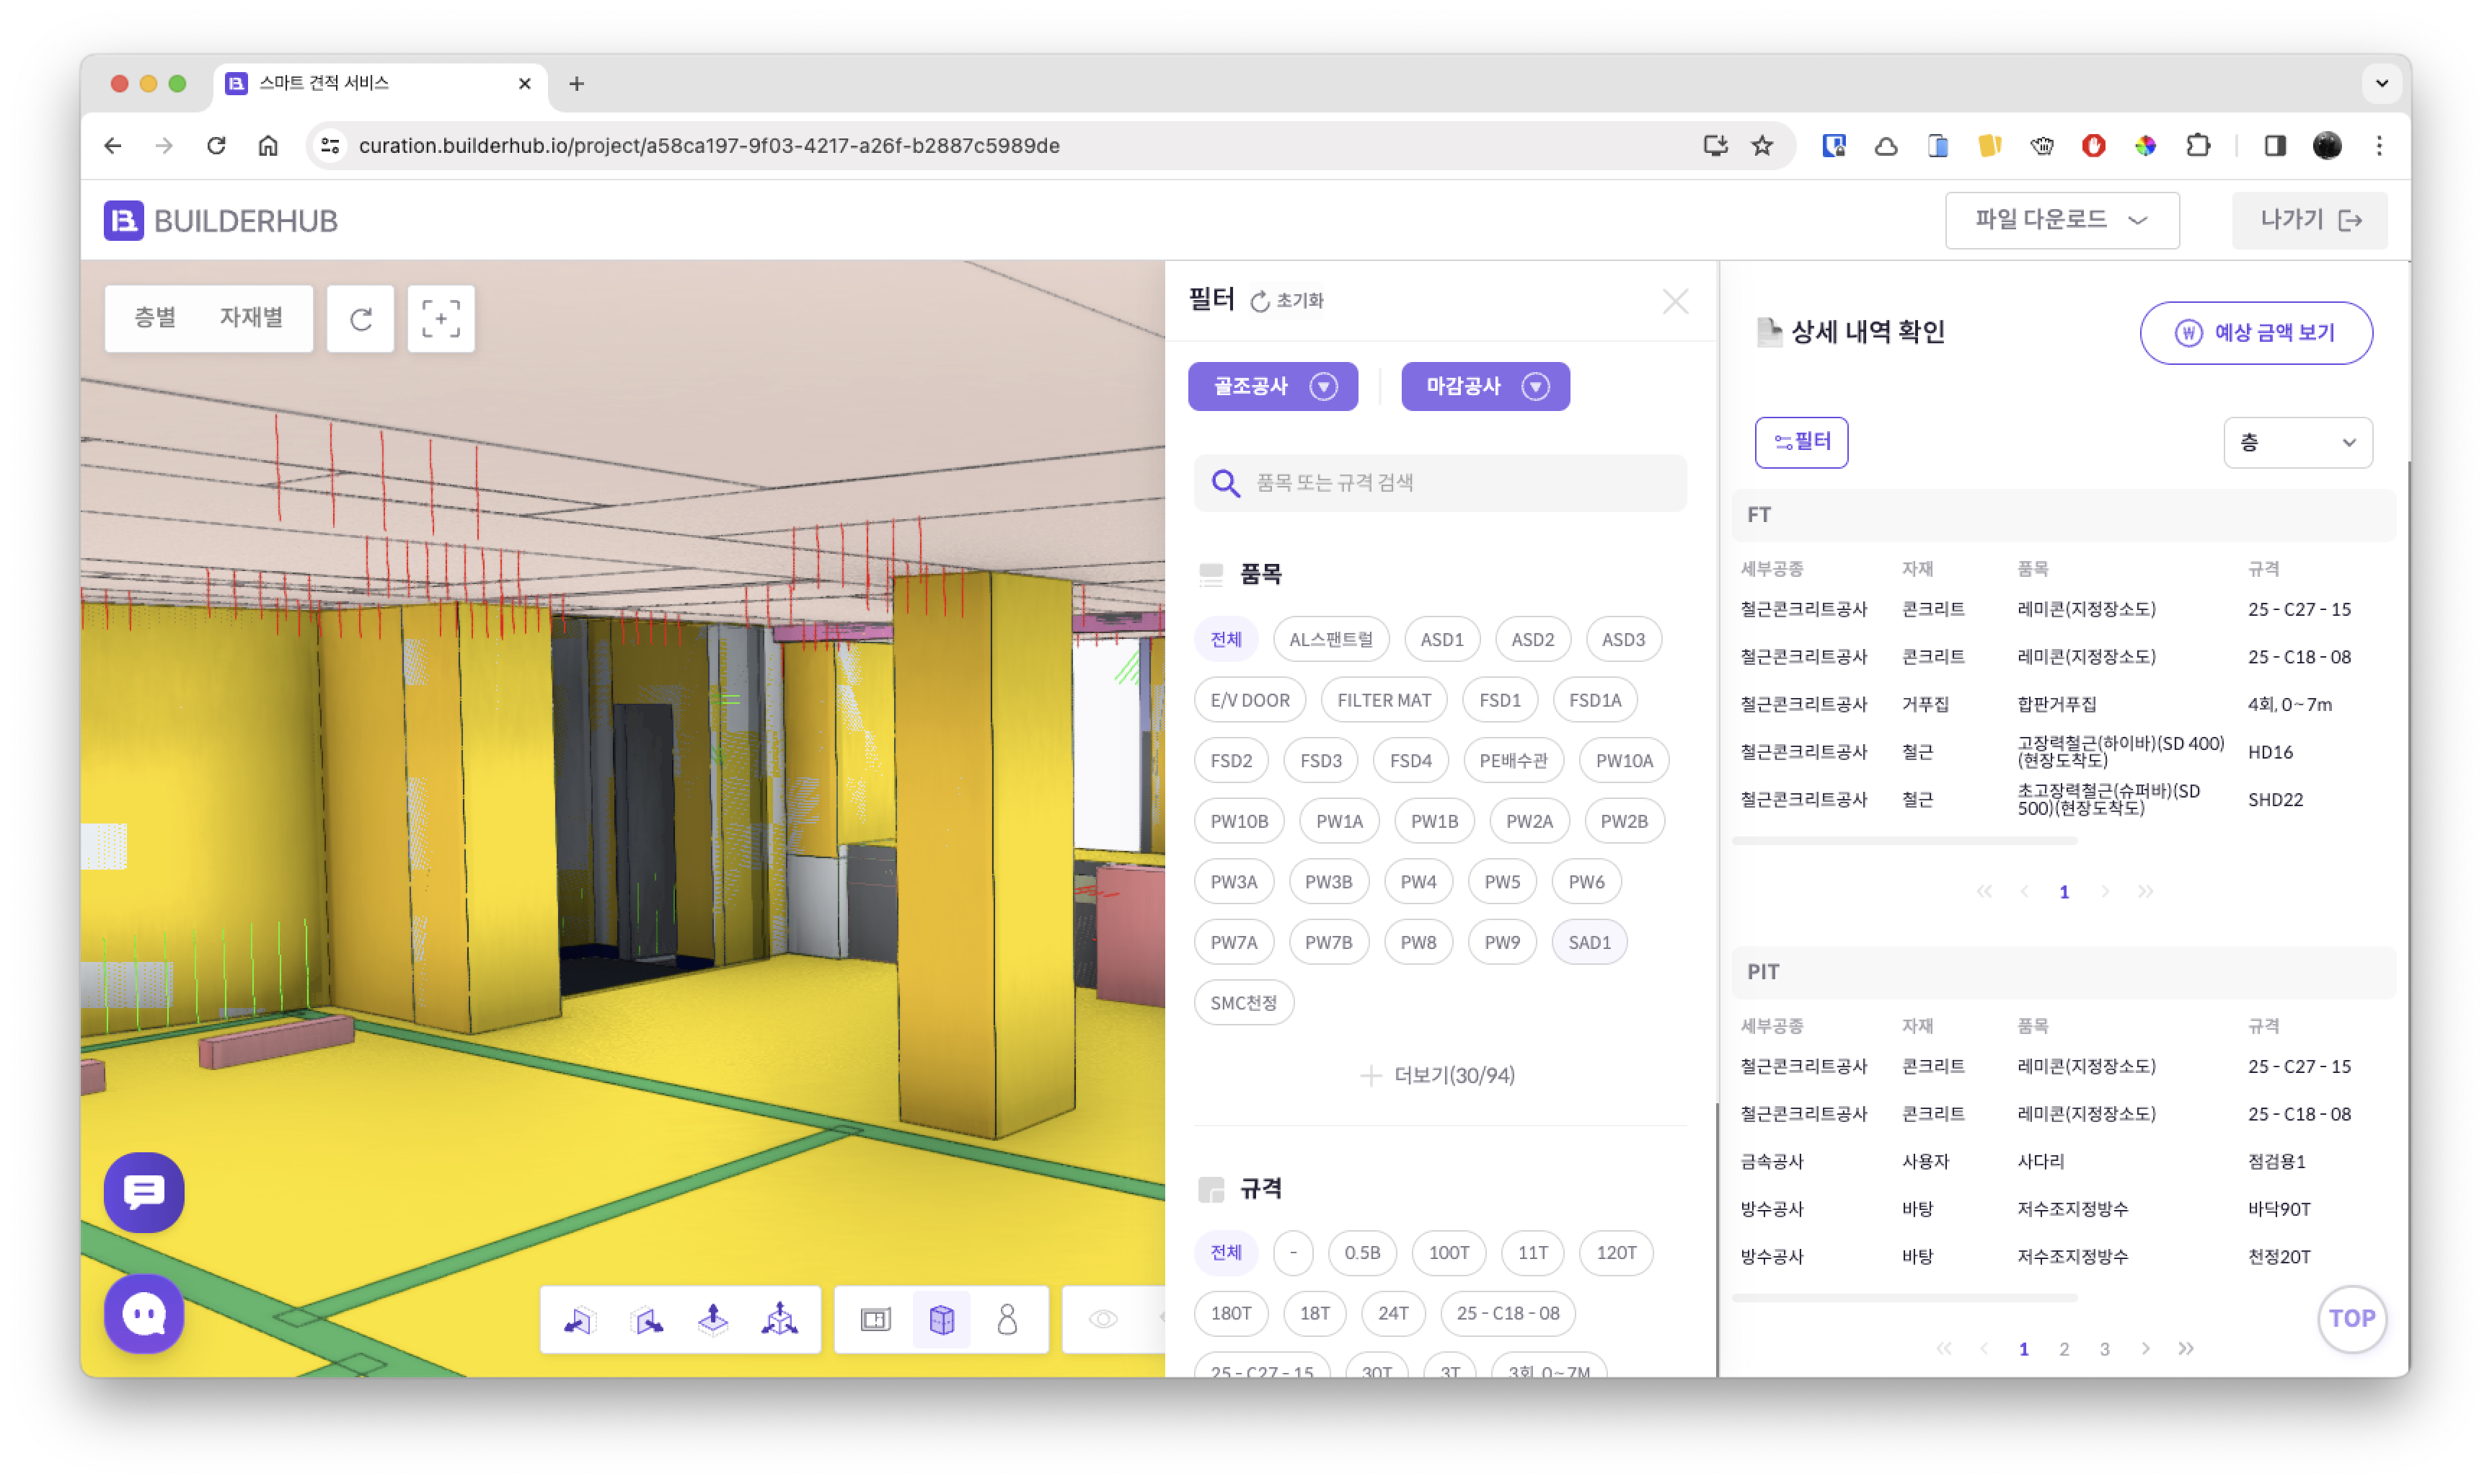
\includegraphics[width=0.35\textwidth]{images/builderhub-curation-filter.png}
				      \caption*{Filtering}
			      }\qquad
			      \parbox{0.35\textwidth}{
				      \centering
				      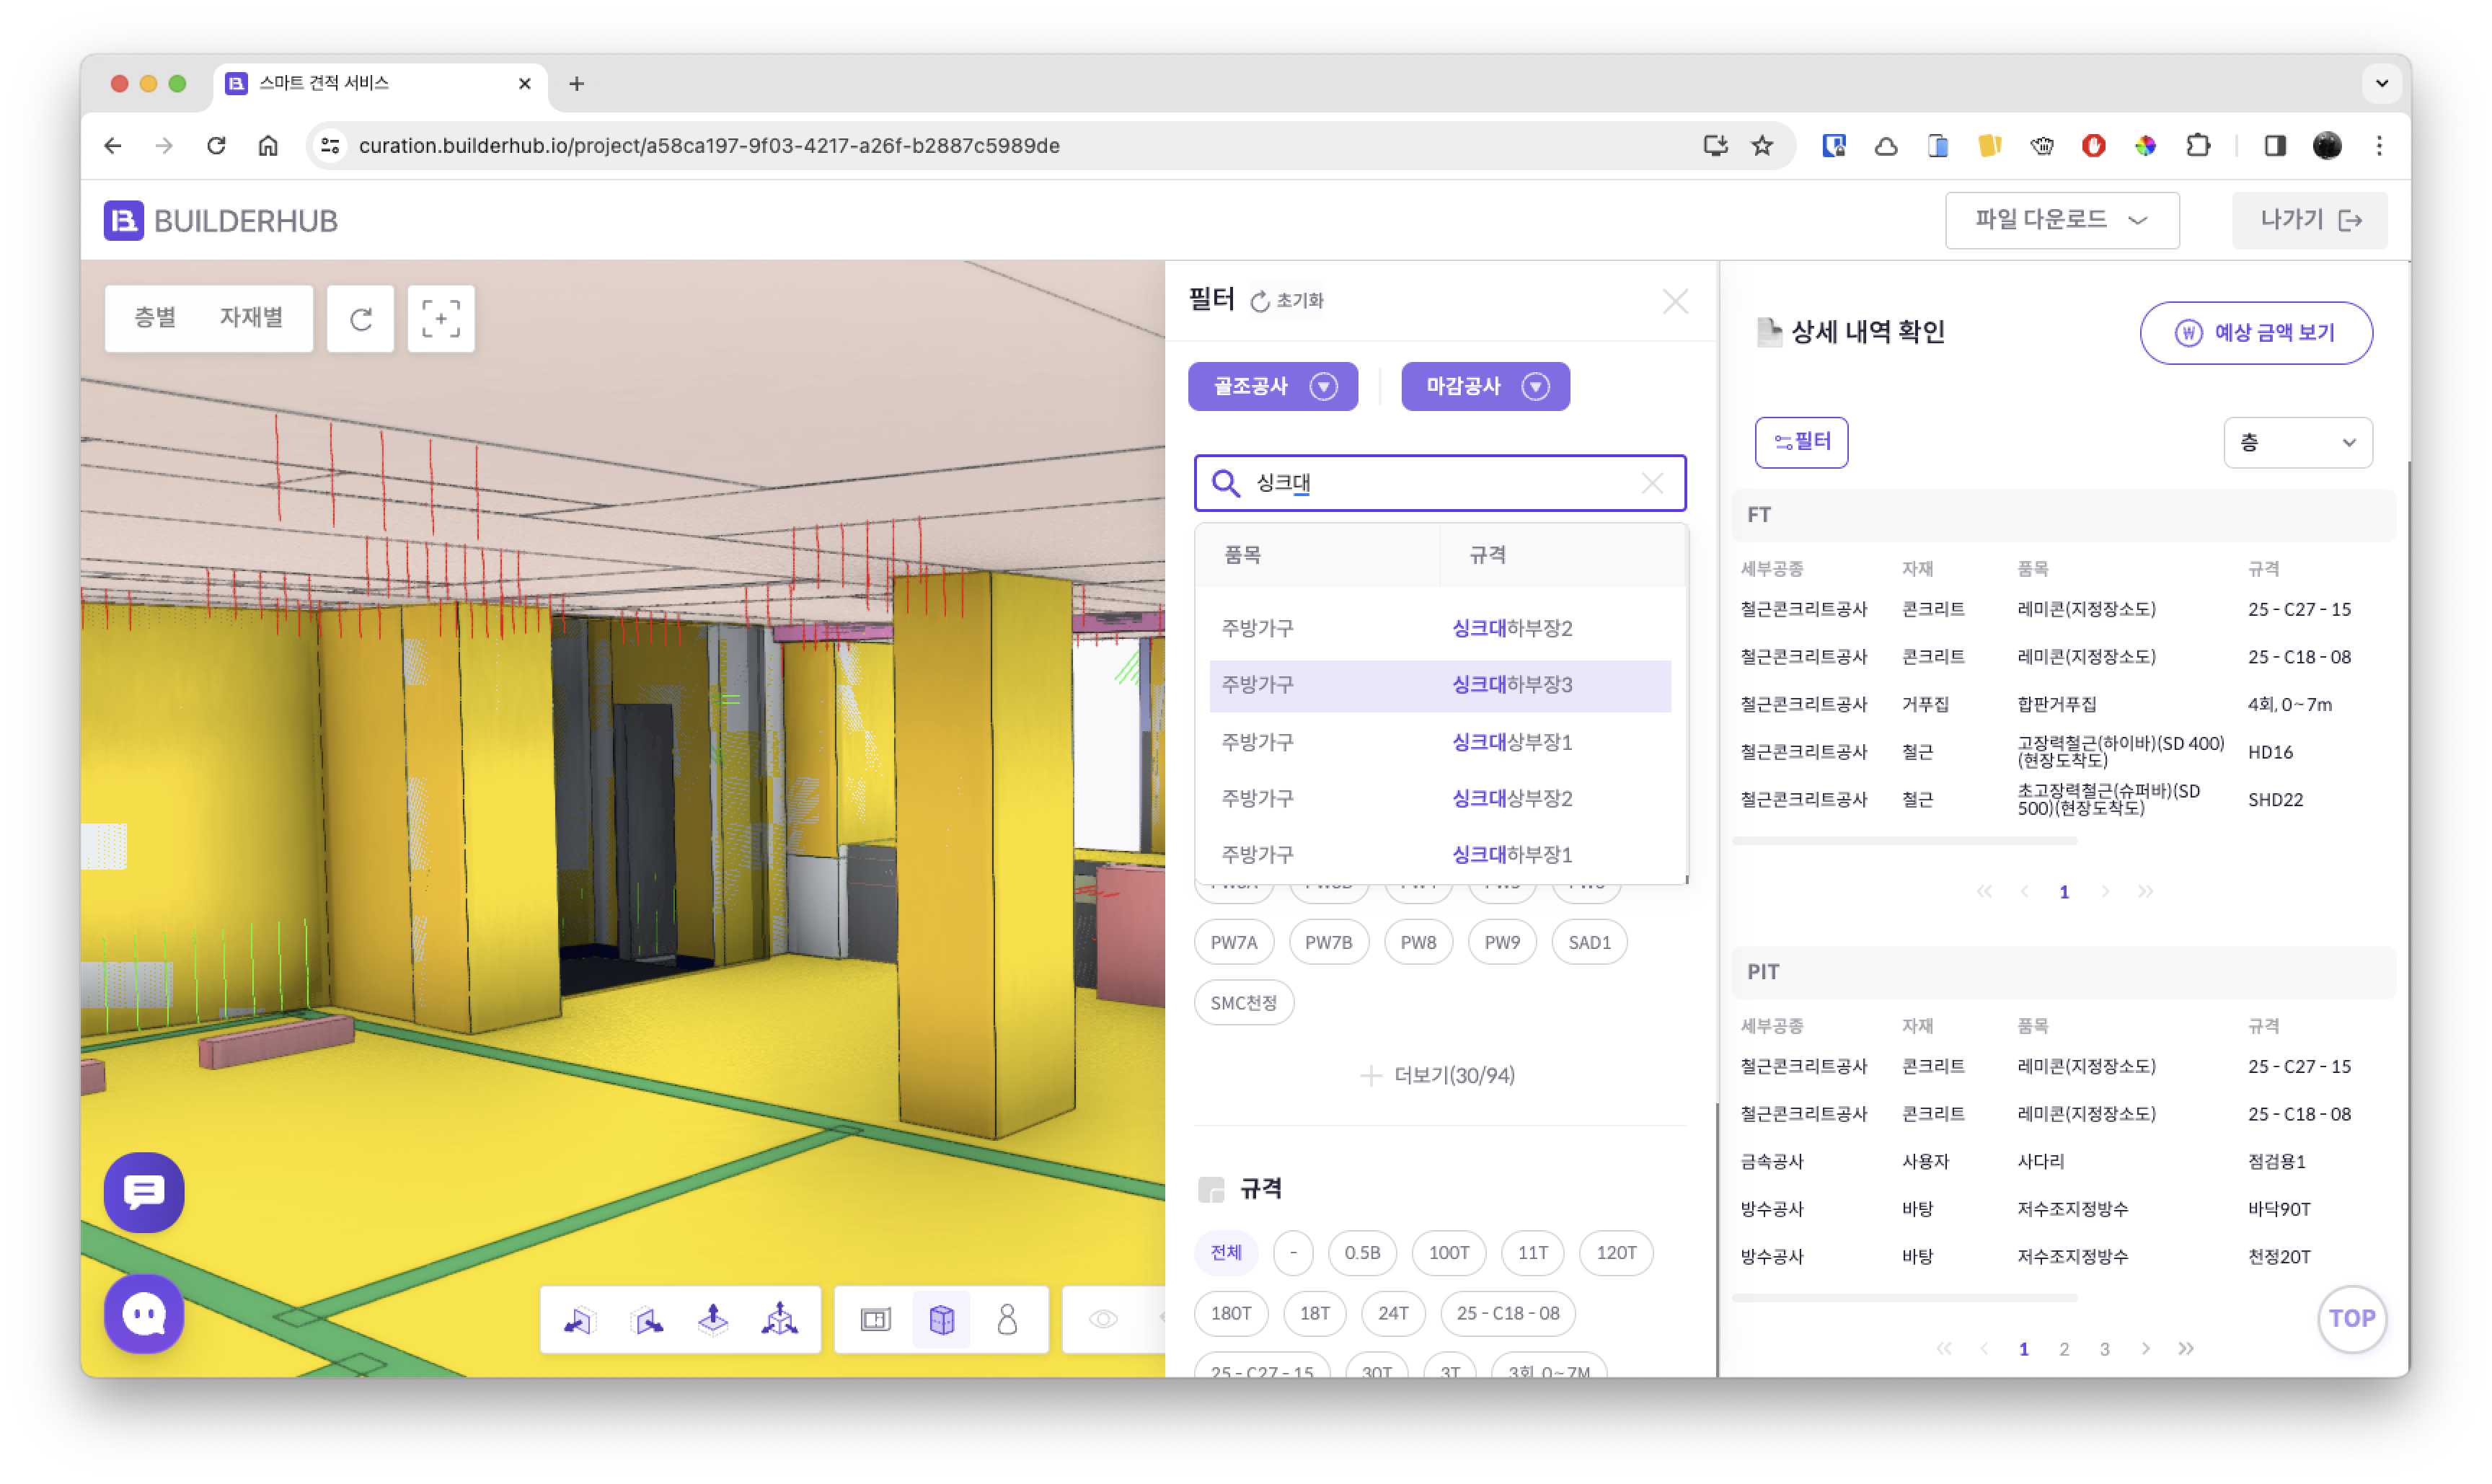
\includegraphics[width=0.35\textwidth]{images/builderhub-curation-filter-search.png}
				      \caption*{Search}
			      }\qquad
			      \parbox{0.35\textwidth}{
				      \centering
				      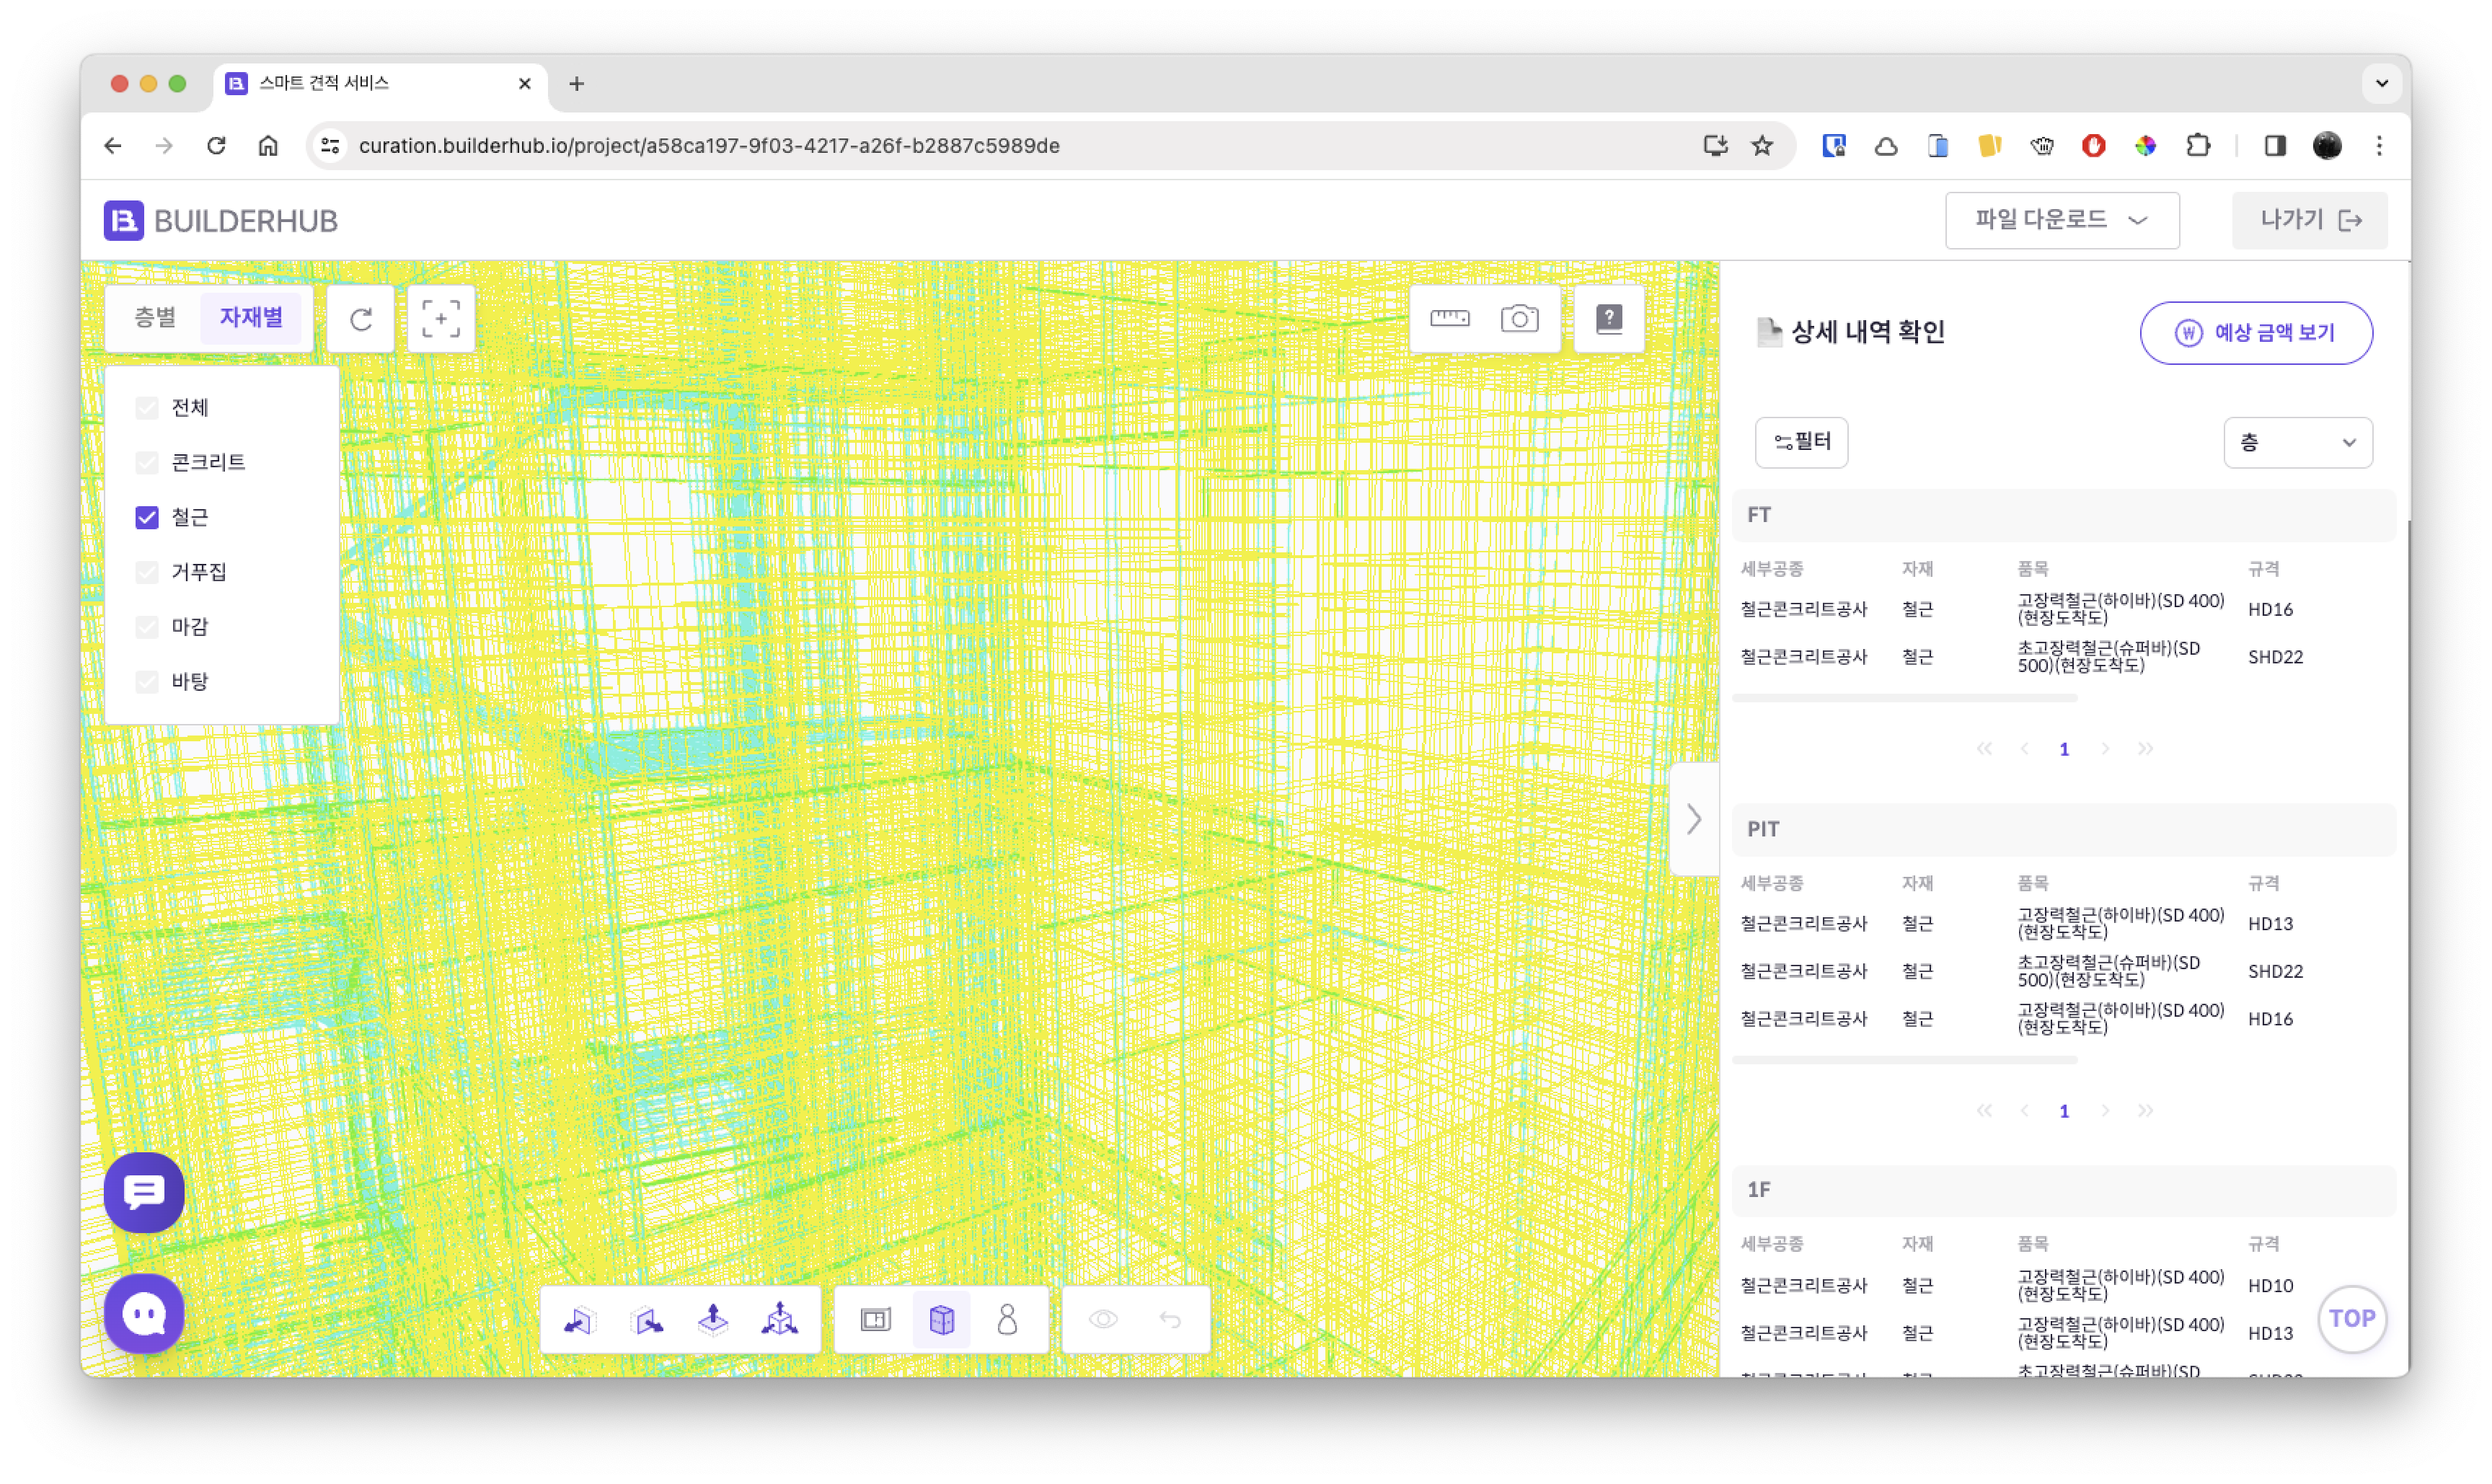
\includegraphics[width=0.35\textwidth]{images/builderhub-curation-filter-material.png}
				      \caption*{Material filter}
			      }\qquad
			      \parbox{0.35\textwidth}{
				      \centering
				      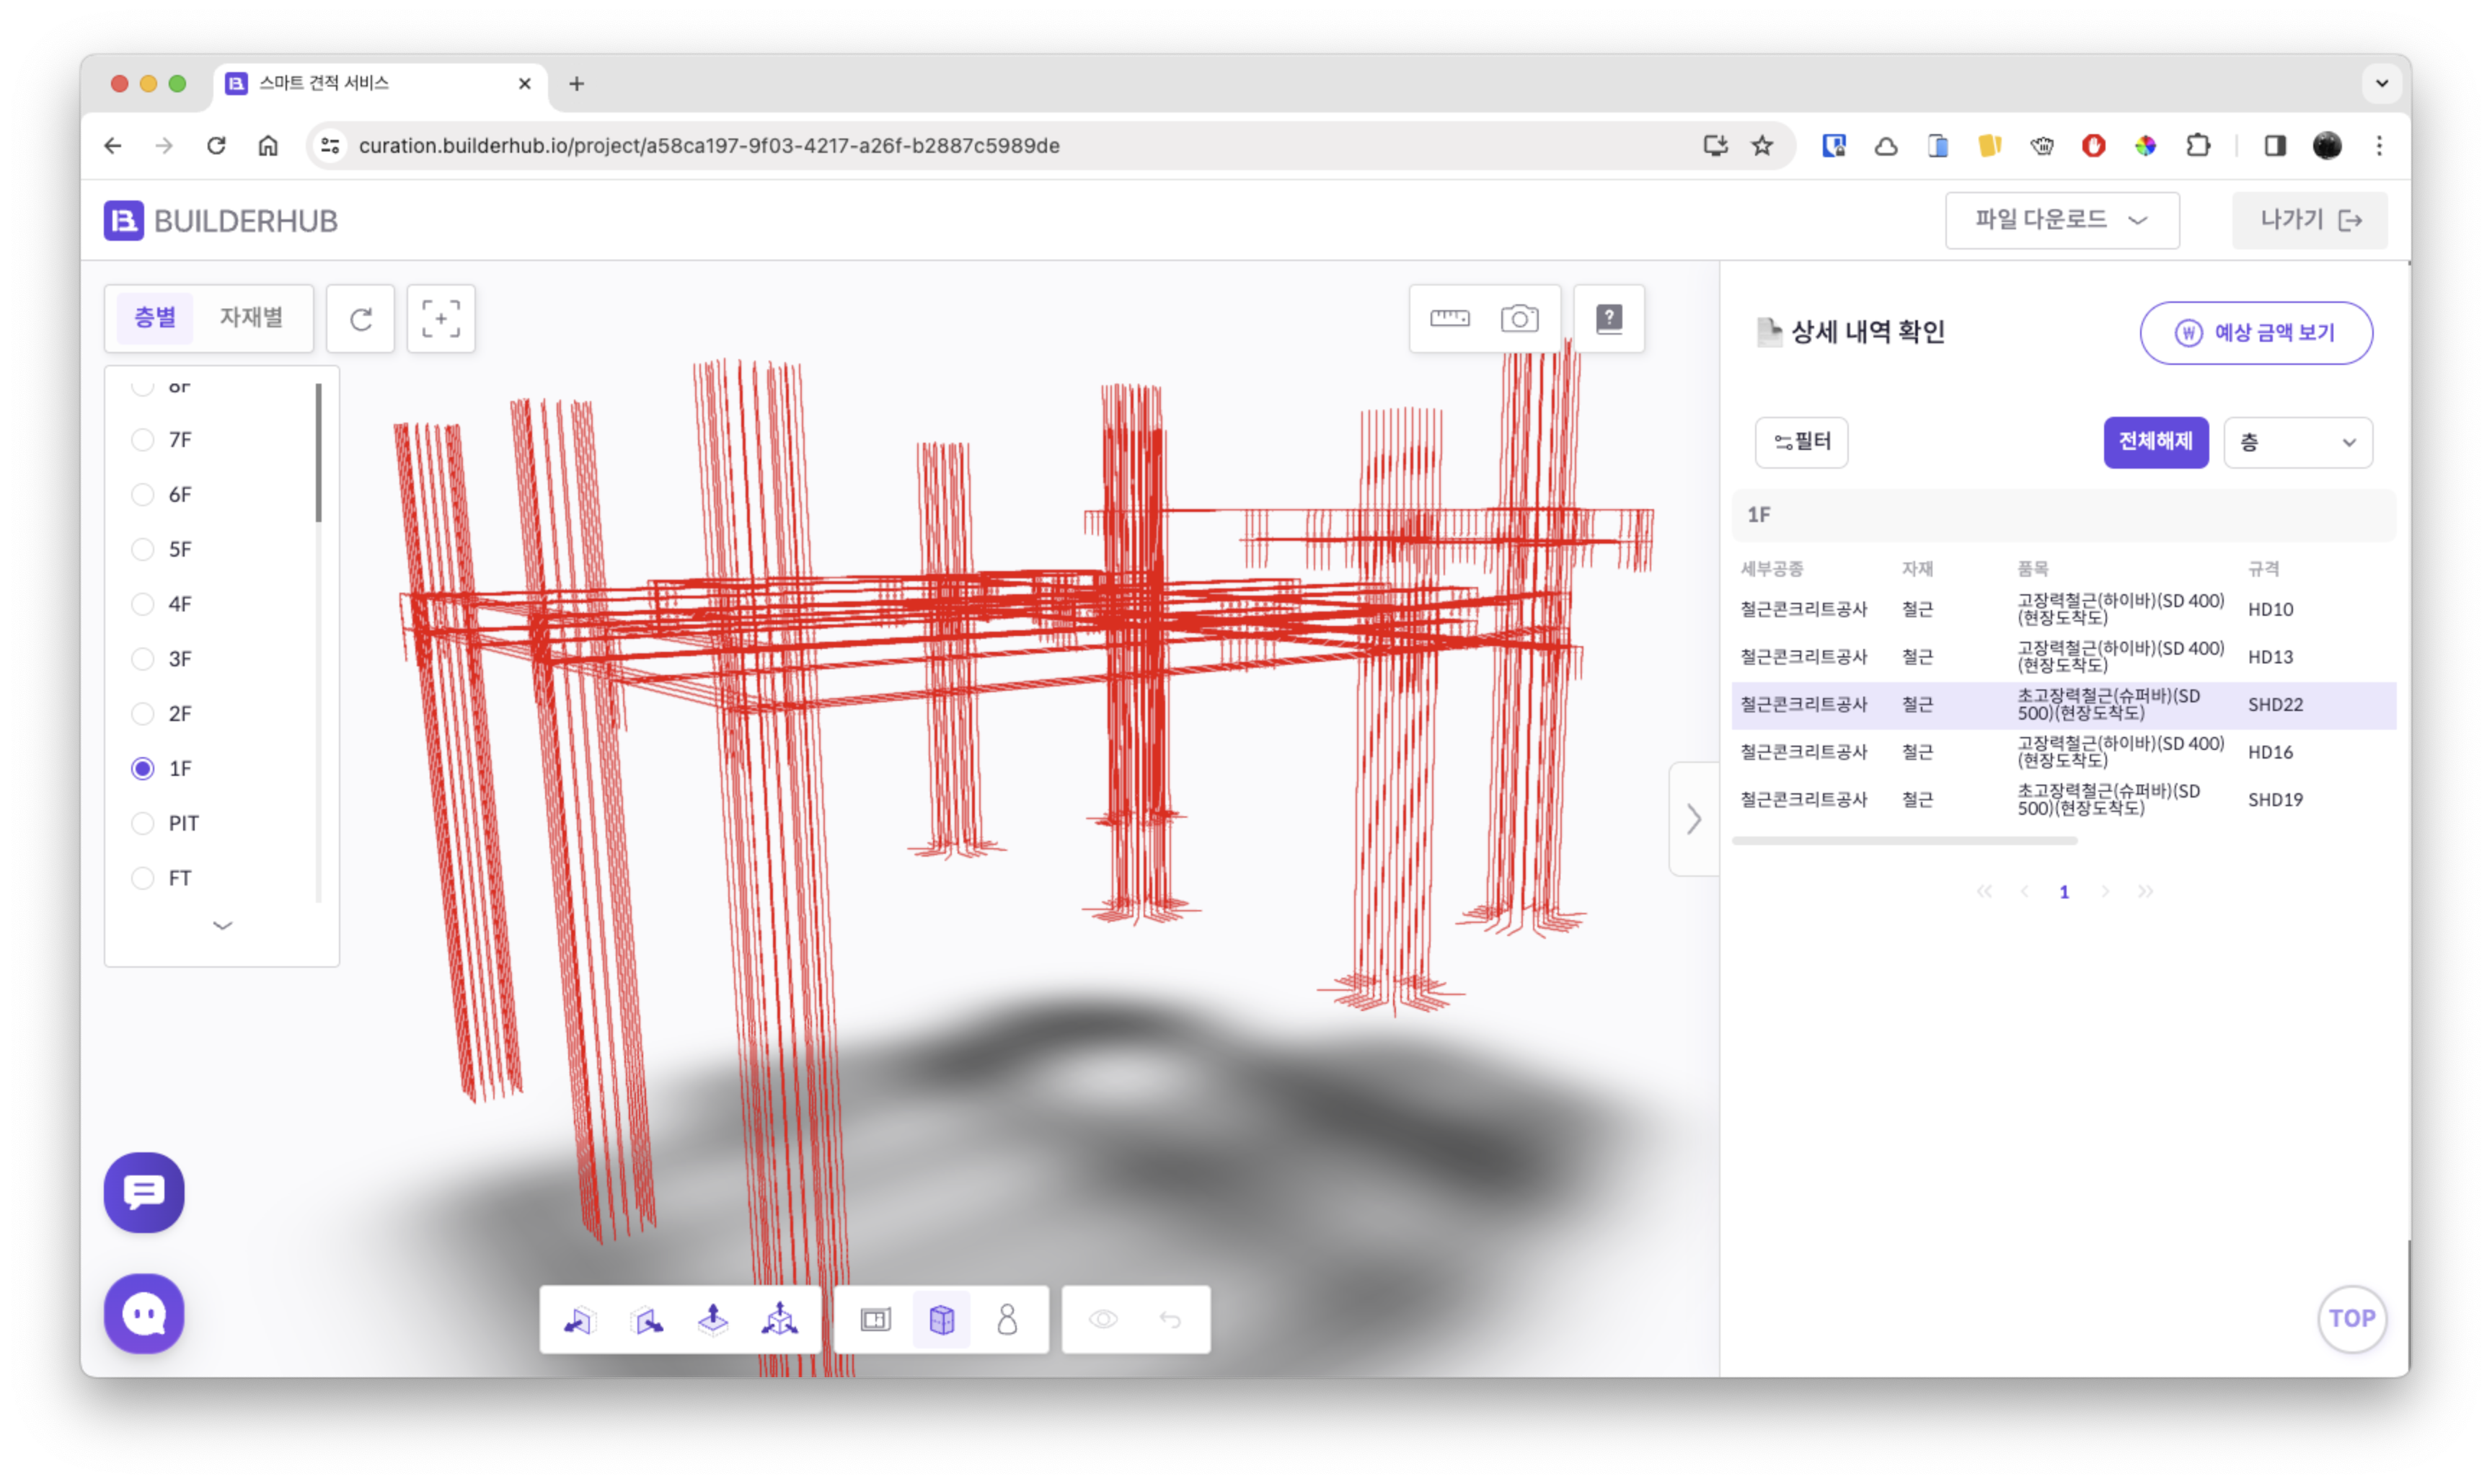
\includegraphics[width=0.35\textwidth]{images/builderhub-curation-filter-table.png}
				      \caption*{Table filter}
			      }
			      \parbox{0.35\textwidth}{
				      \centering
				      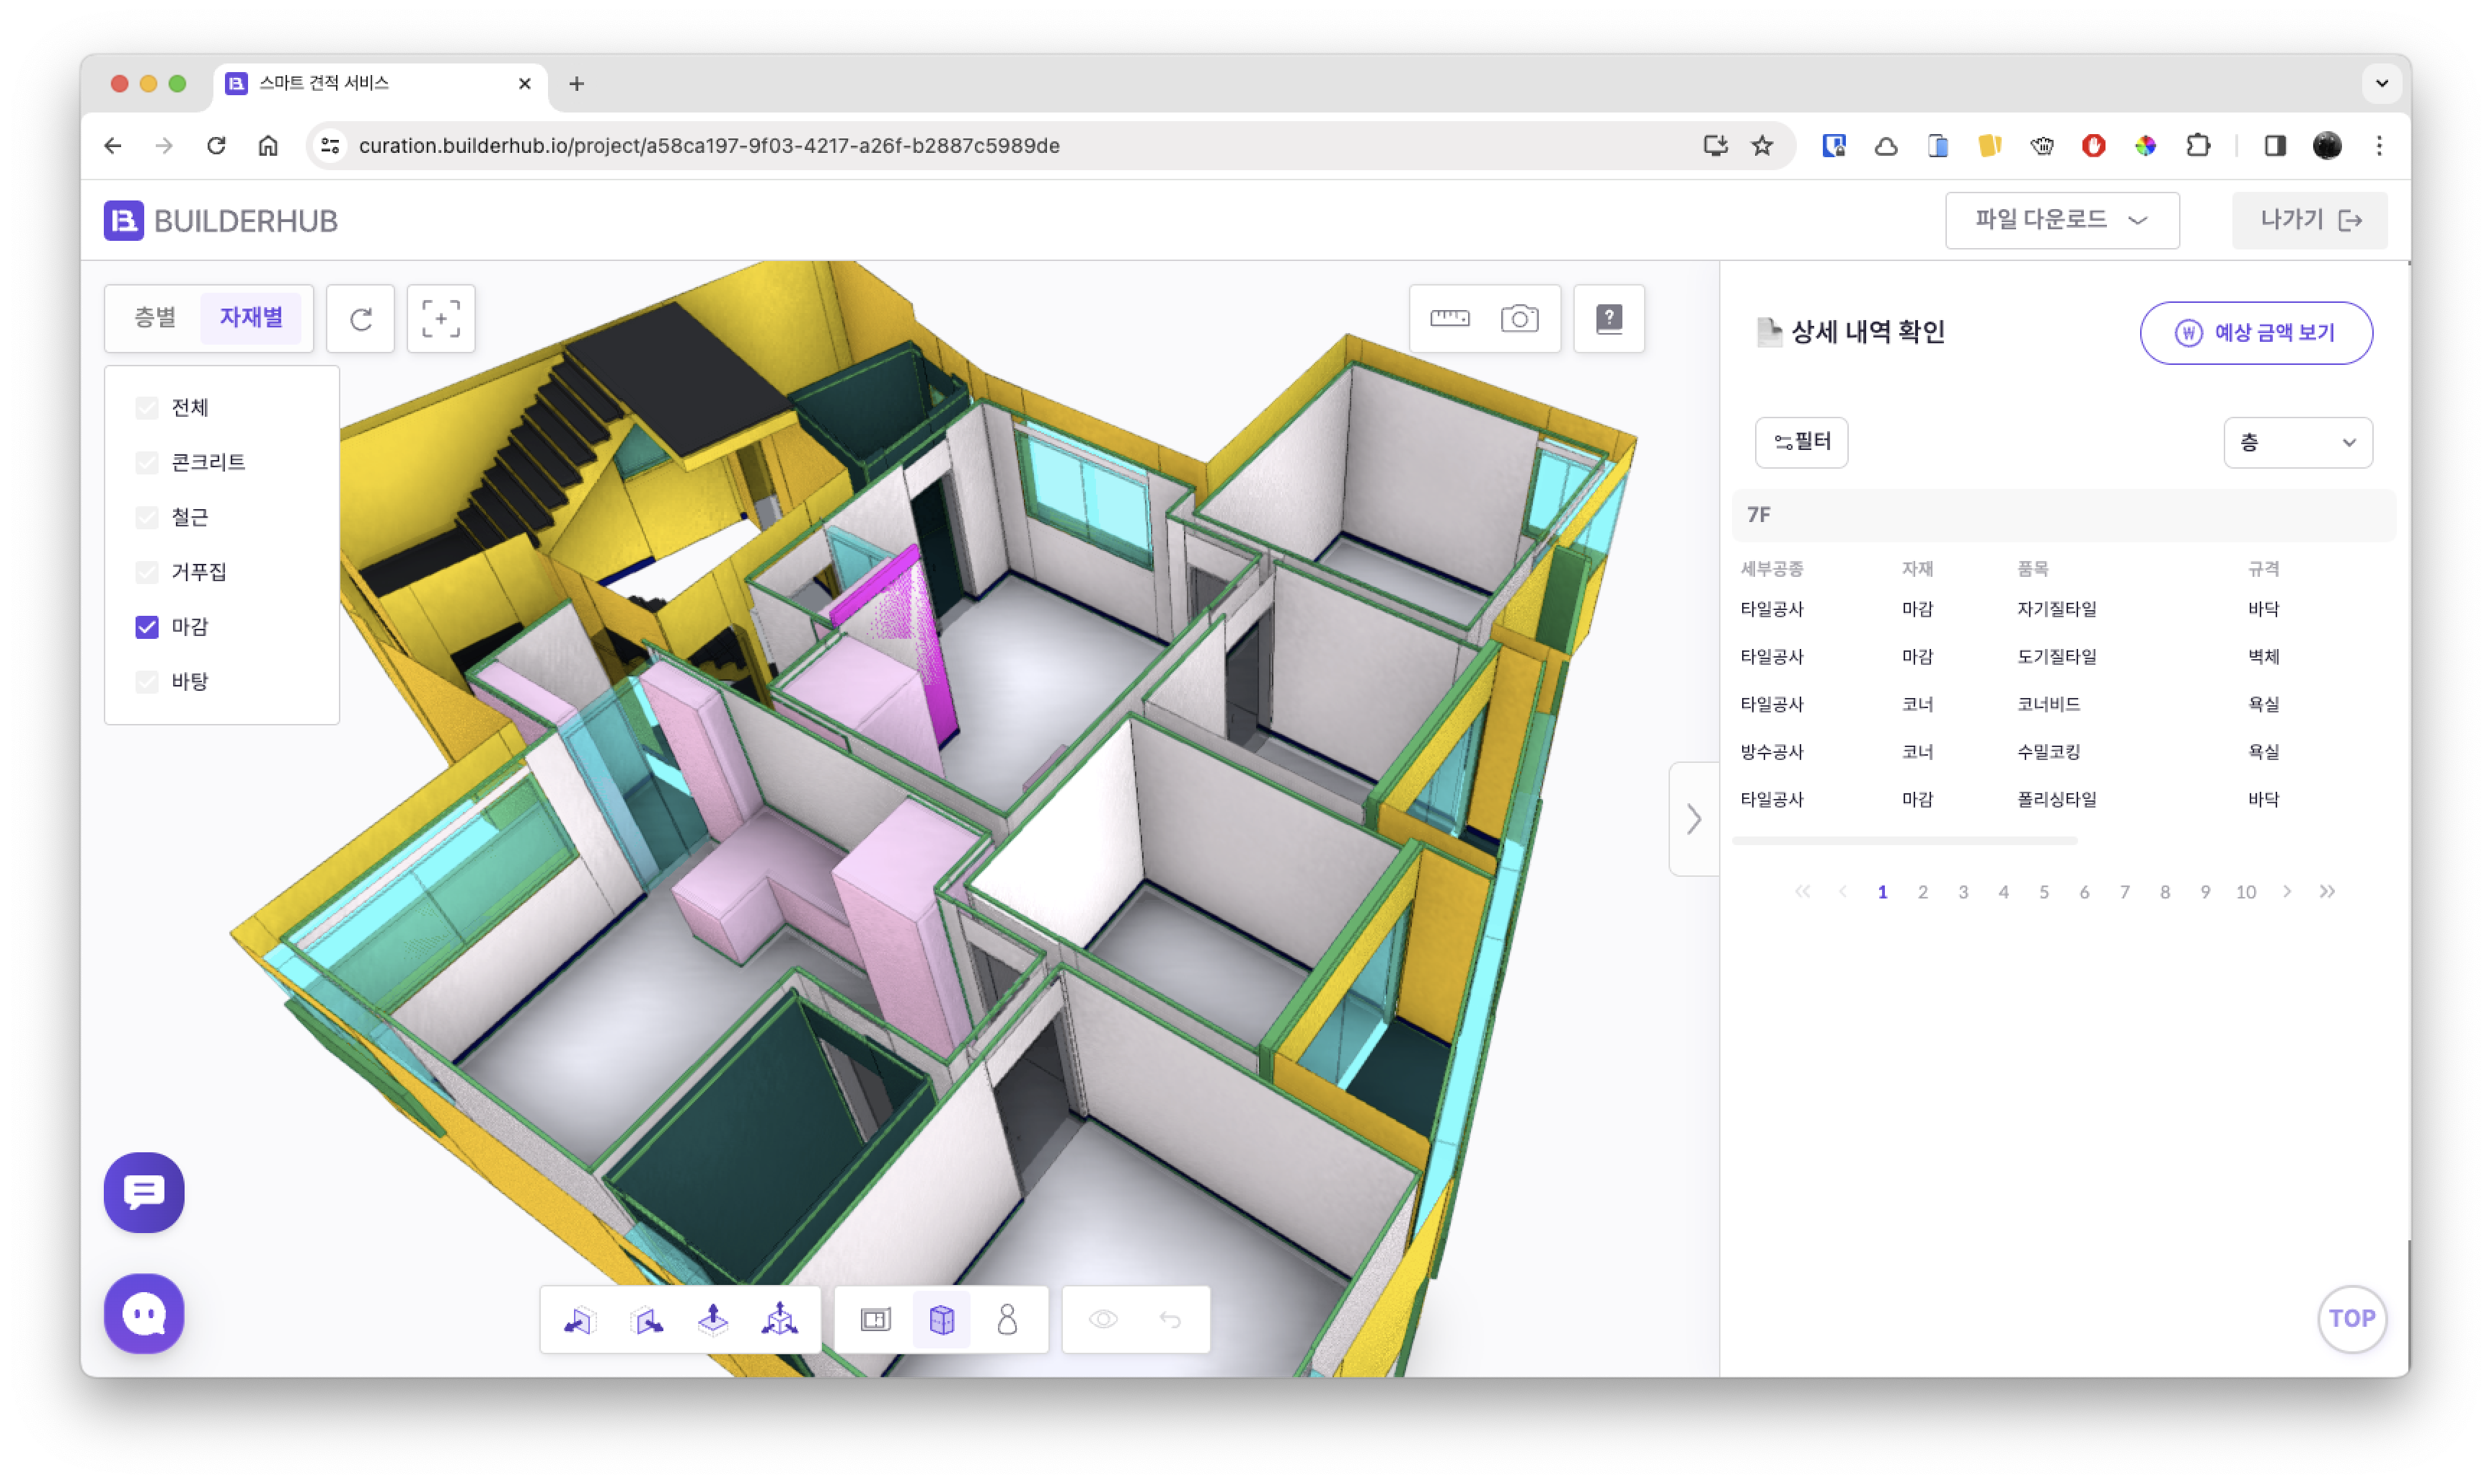
\includegraphics[width=0.35\textwidth]{images/builderhub-curation-filter-floor.png}
				      \caption*{Floor filter}
			      }\qquad
			      \parbox{0.35\textwidth}{
				      \centering
				      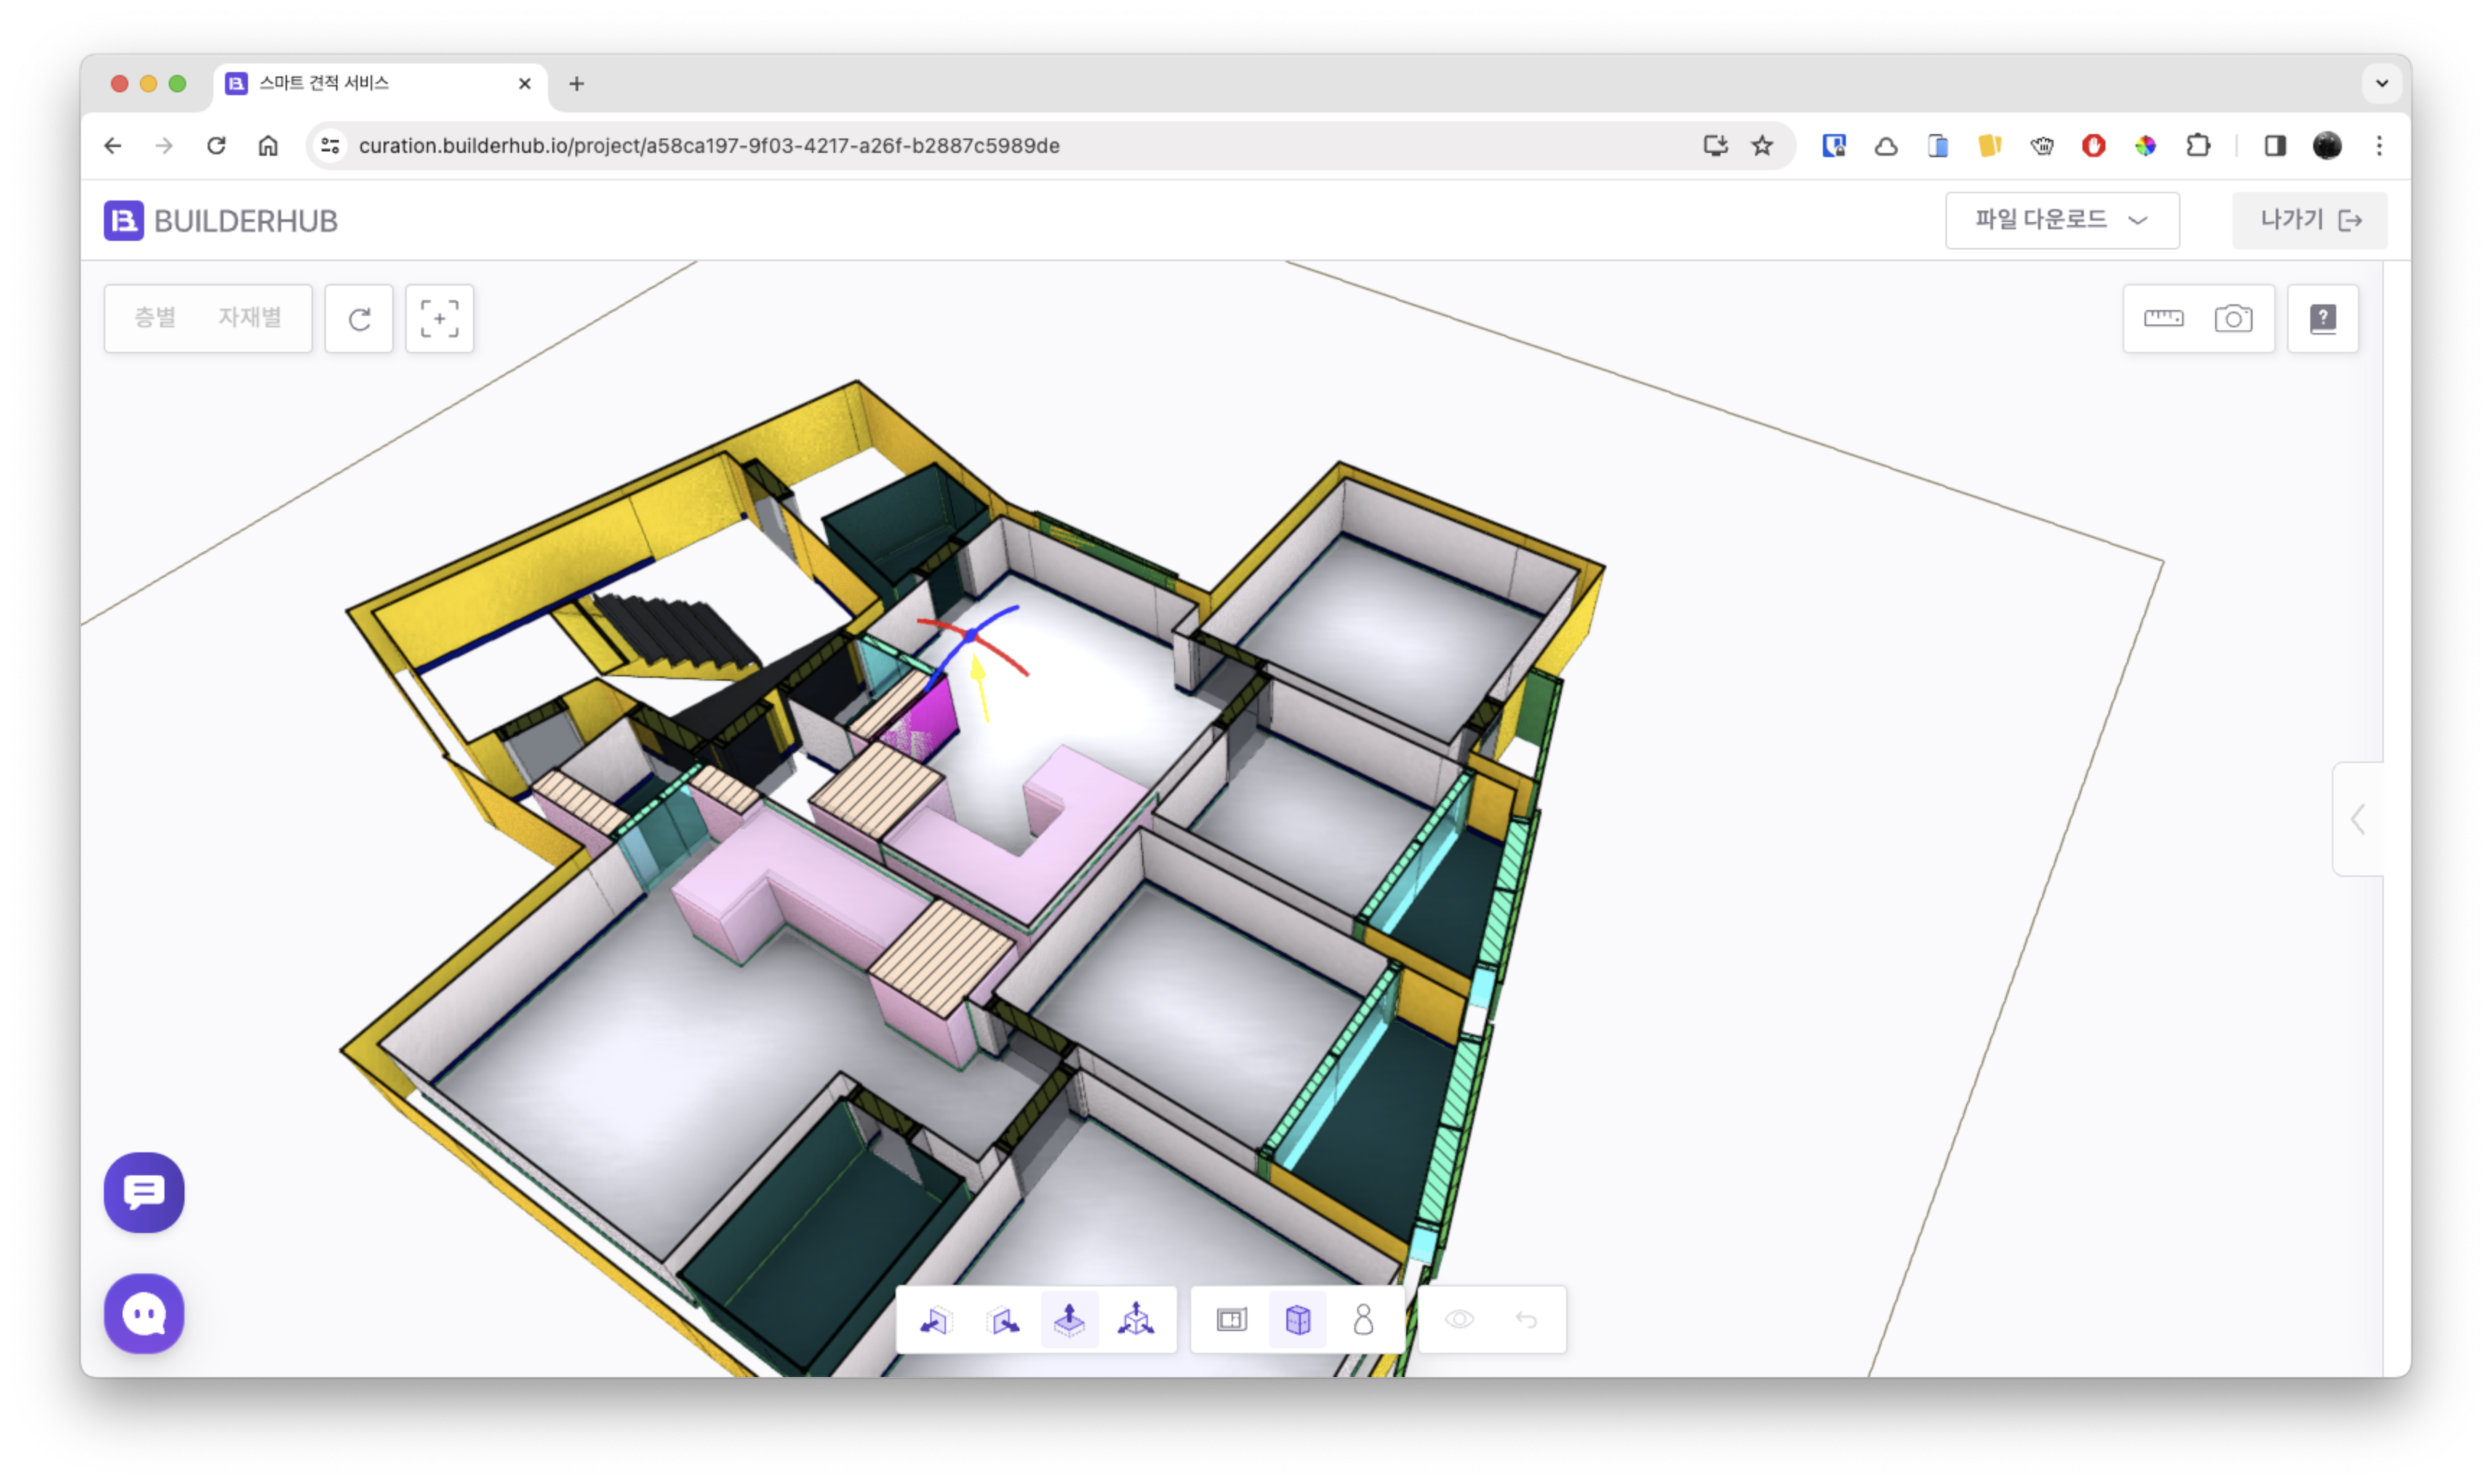
\includegraphics[width=0.35\textwidth]{images/builderhub-curation-section-view.png}
				      \caption*{Section view}
			      }\qquad
			      \parbox{0.35\textwidth}{
				      \centering
				      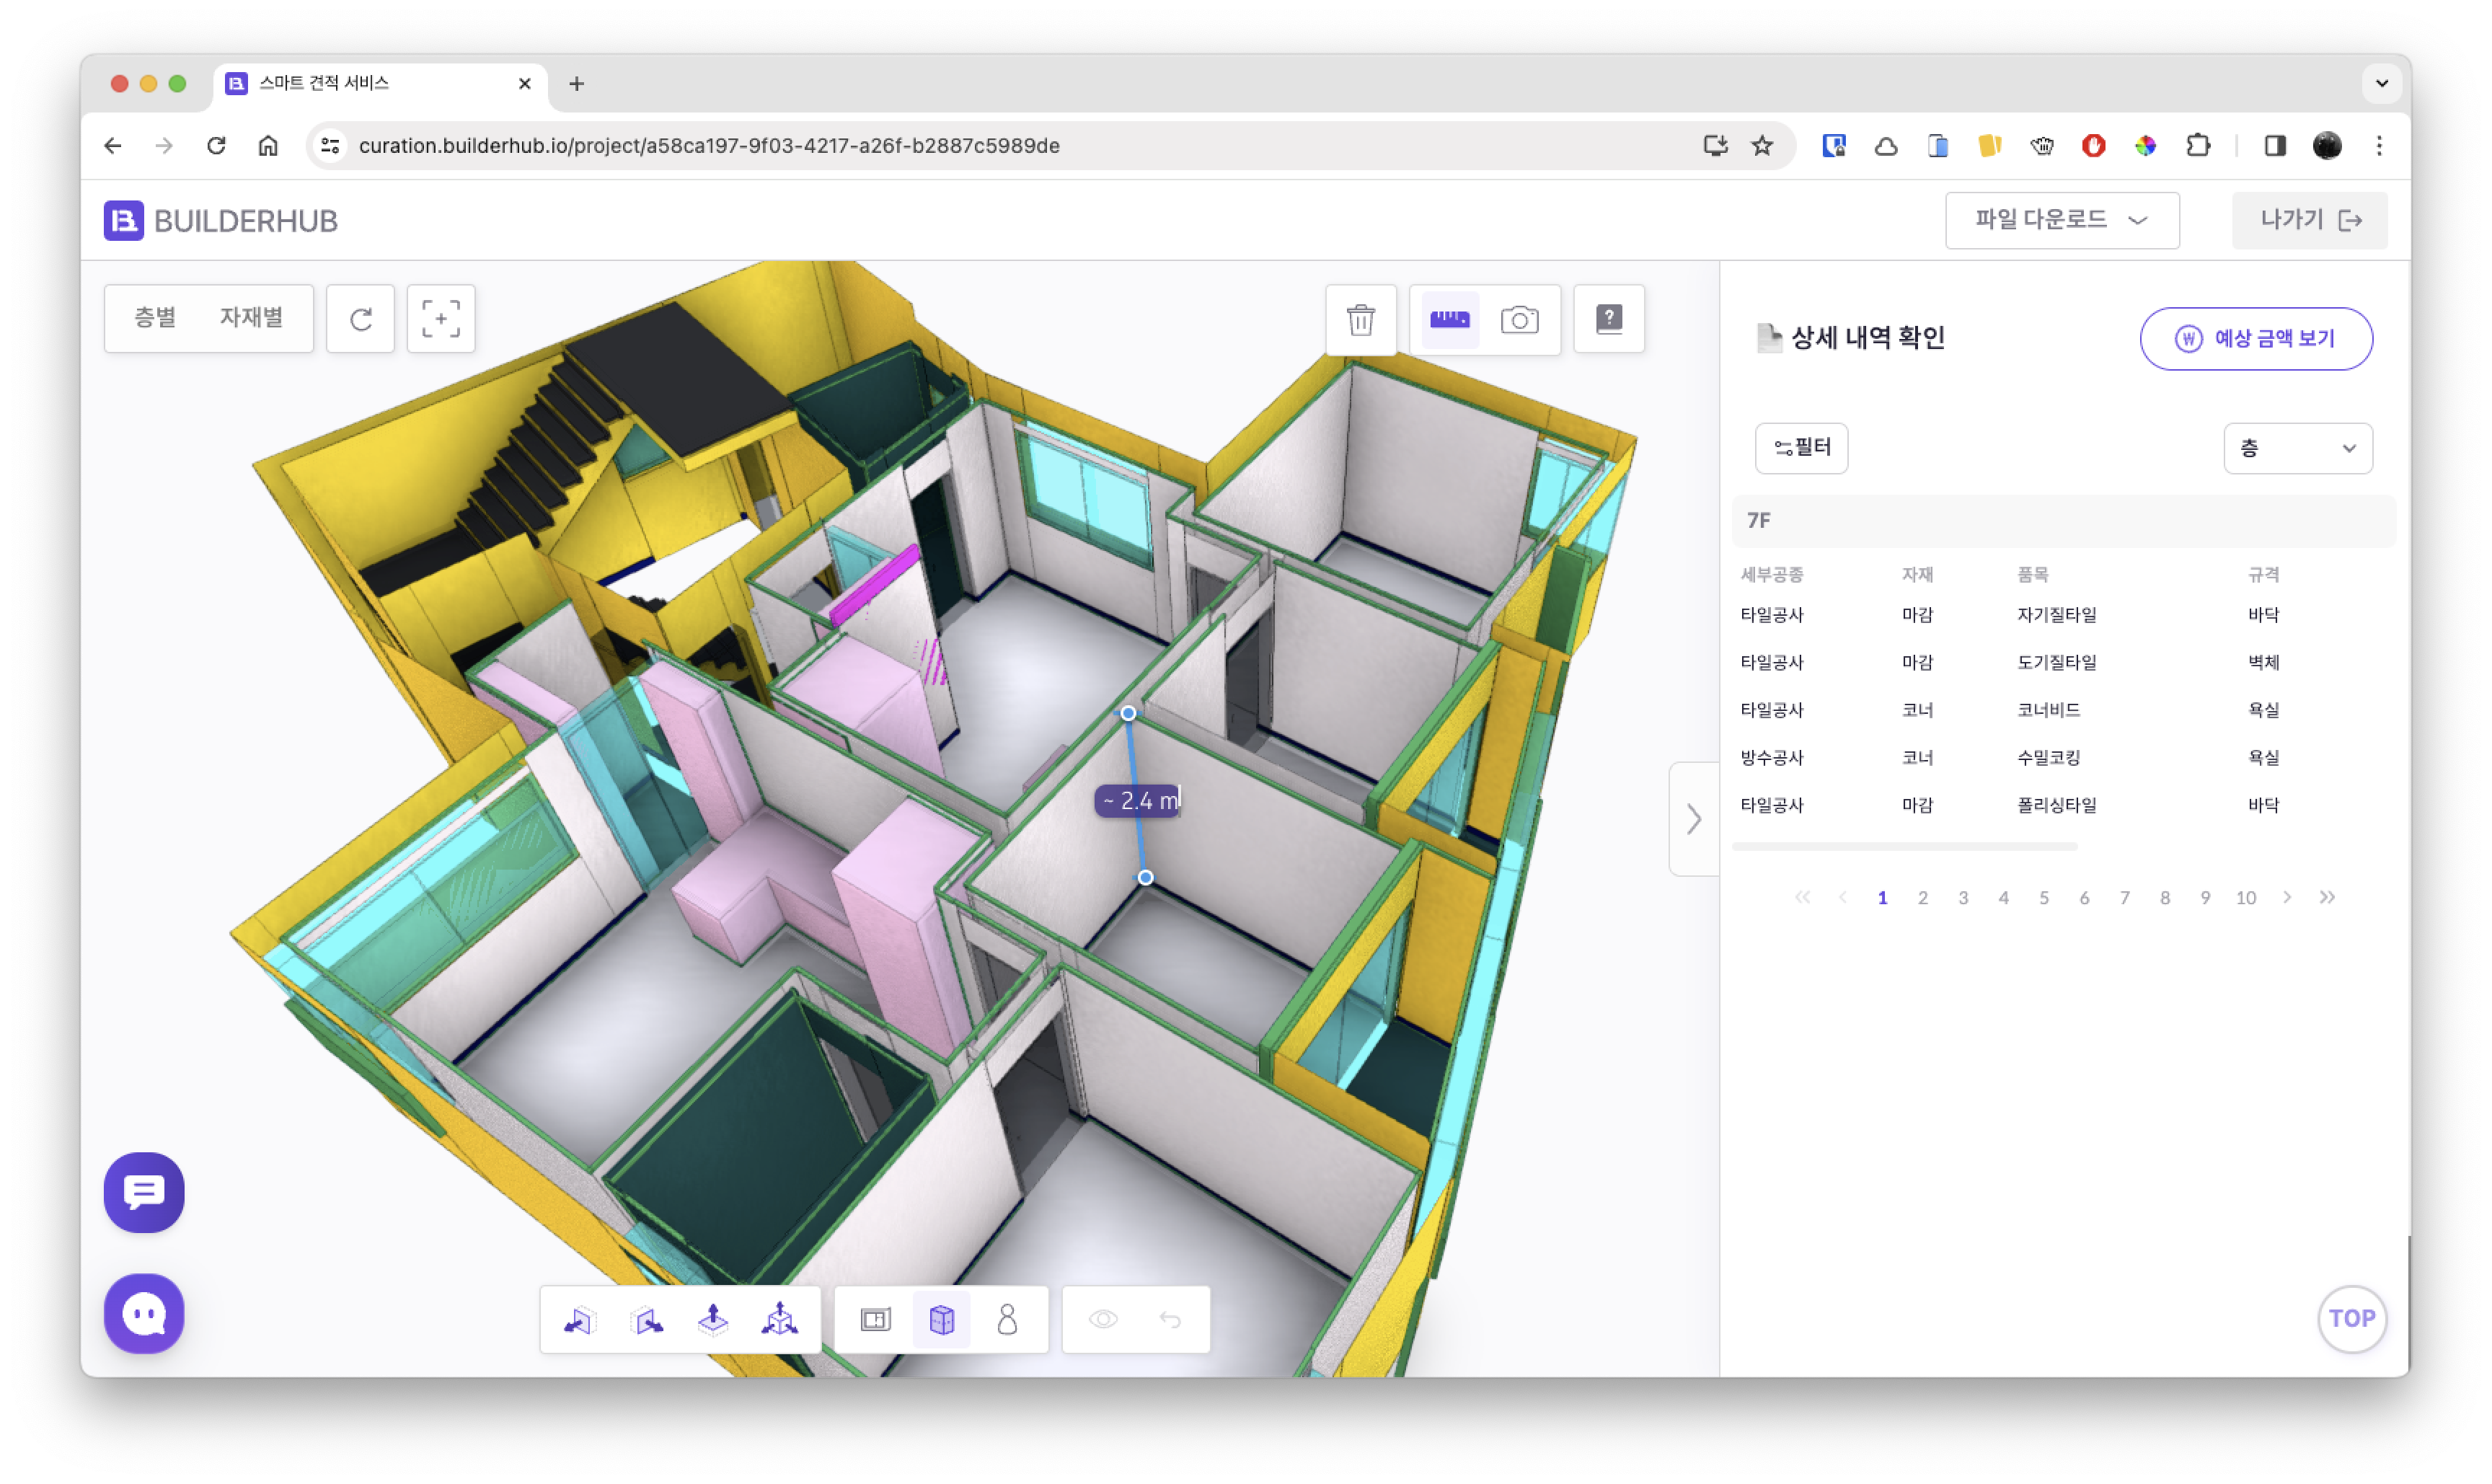
\includegraphics[width=0.35\textwidth]{images/builderhub-curation-measurement.png}
				      \caption*{Measurement}
			      }\qquad
			      \parbox{0.35\textwidth}{
				      \centering
				      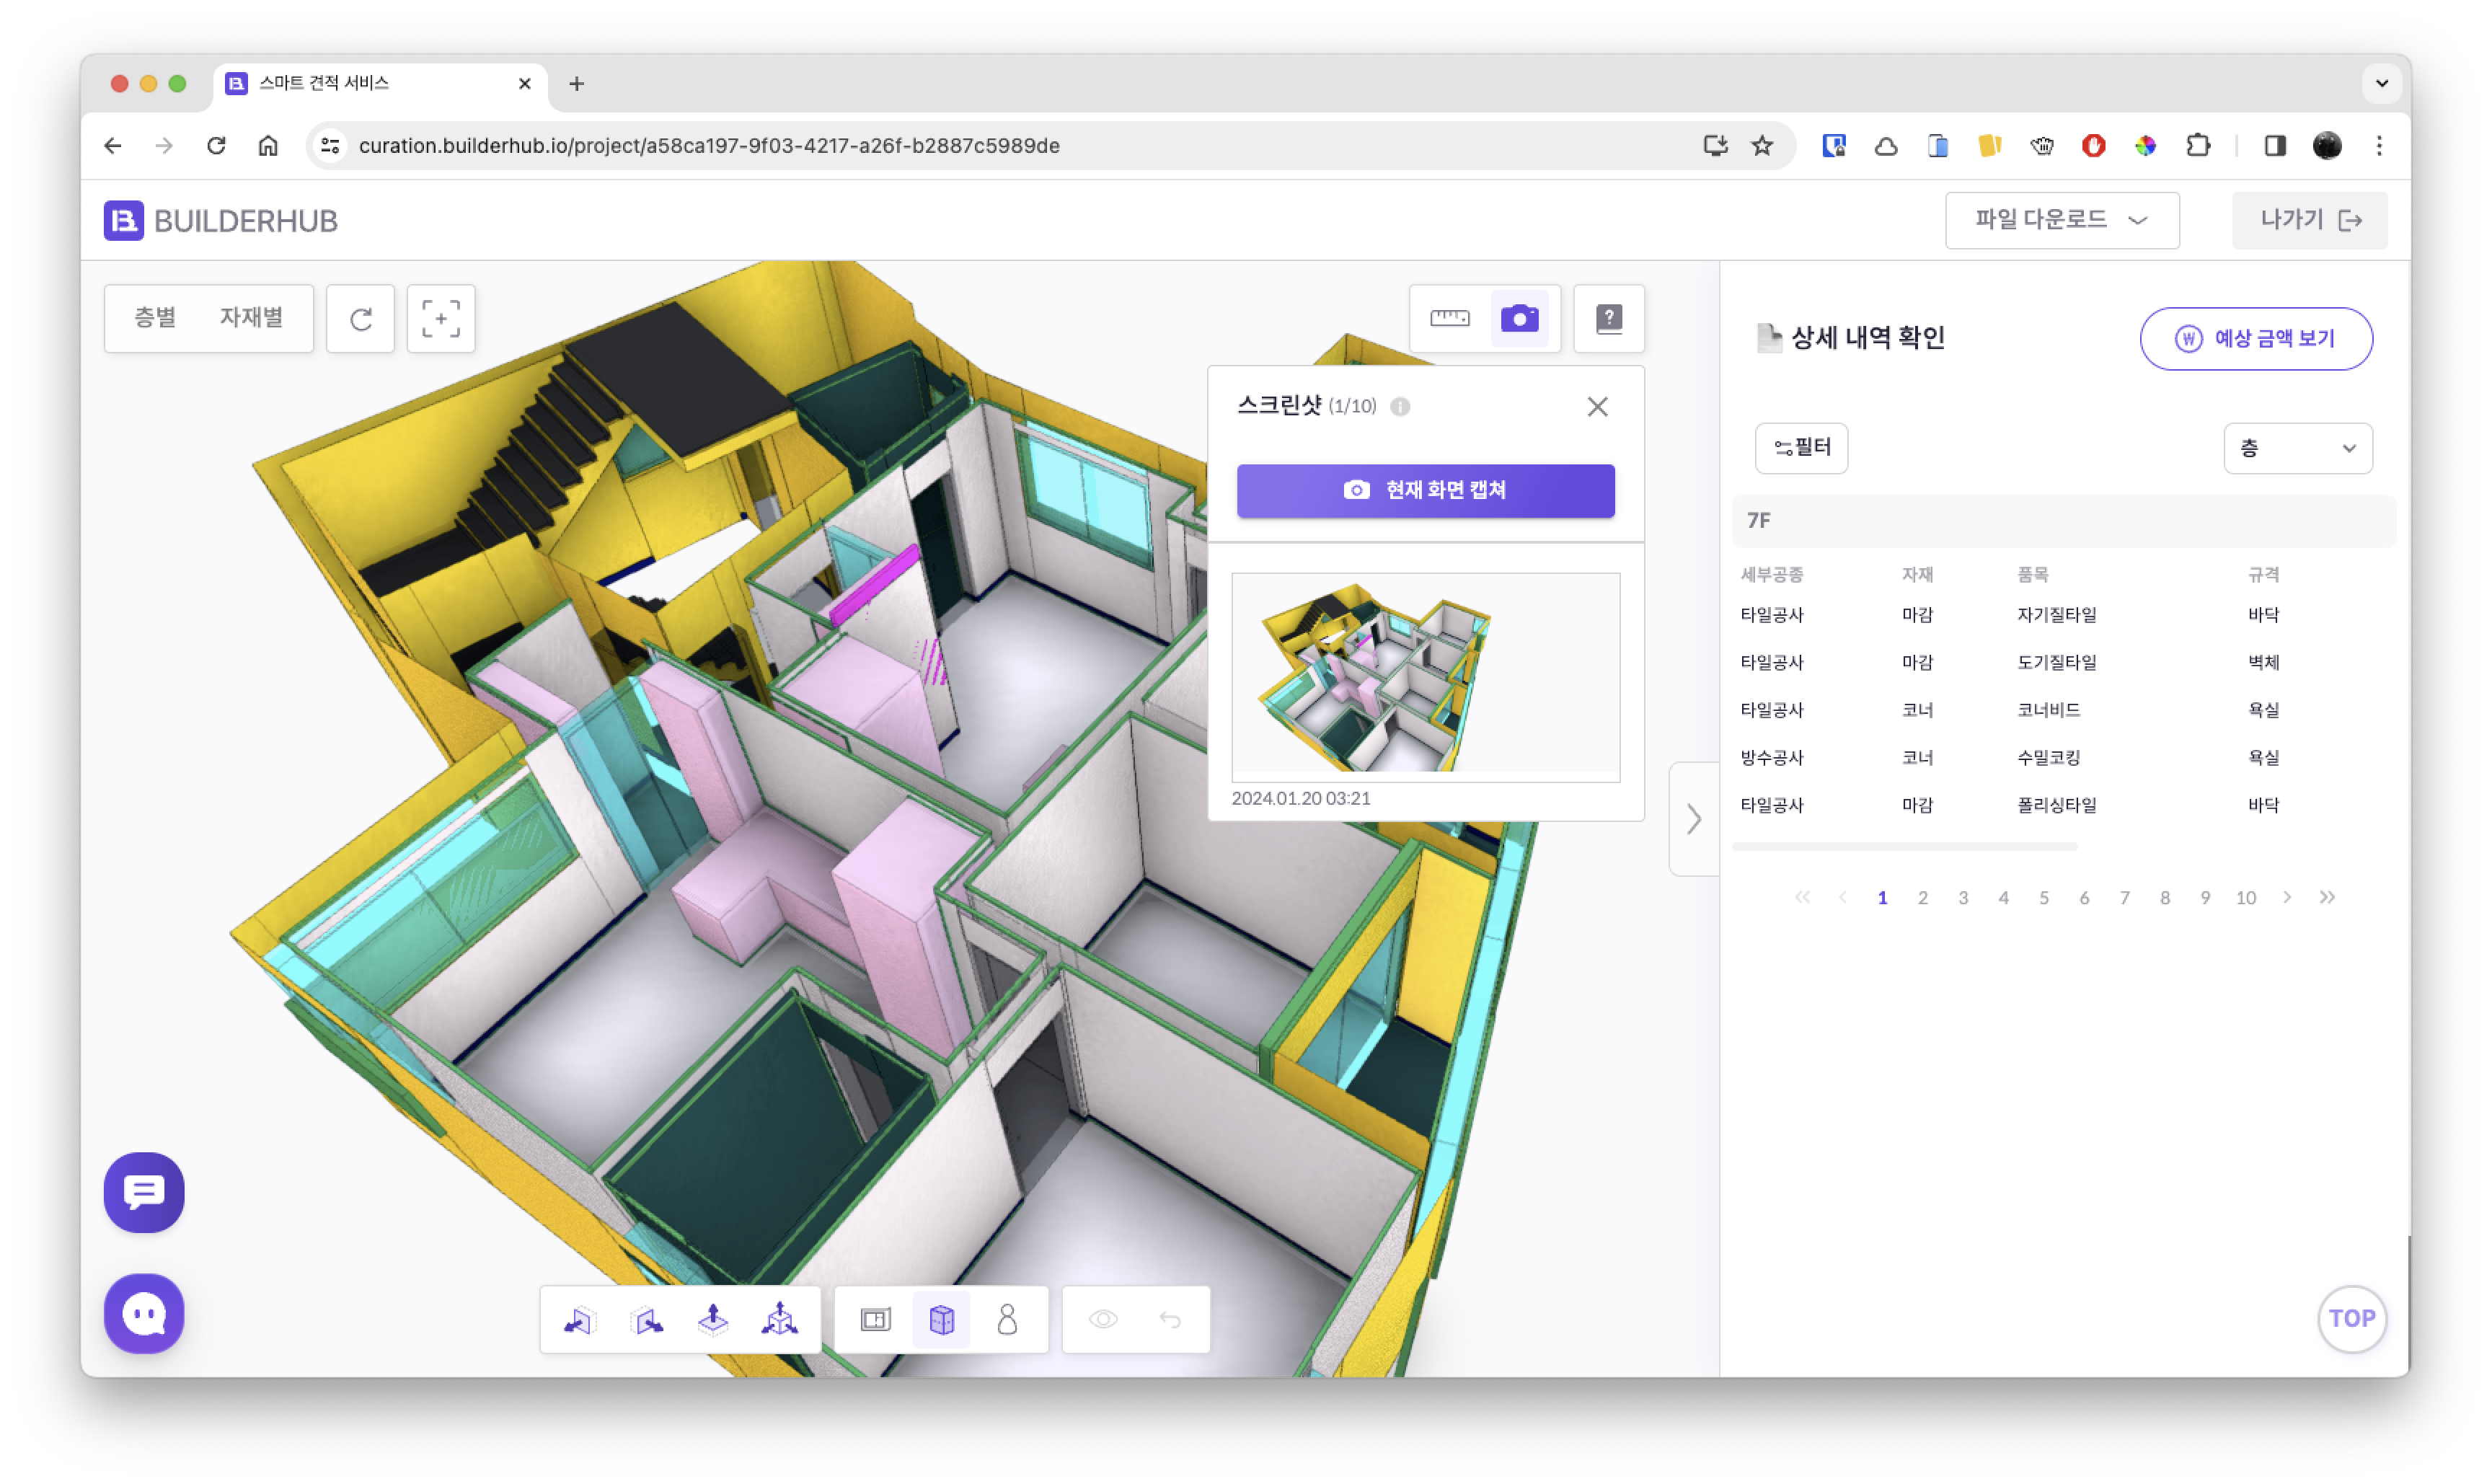
\includegraphics[width=0.35\textwidth]{images/builderhub-curation-screenshot.png}
				      \caption*{Screen Capture}
			      }
			      \parbox{0.35\textwidth}{
				      \centering
				      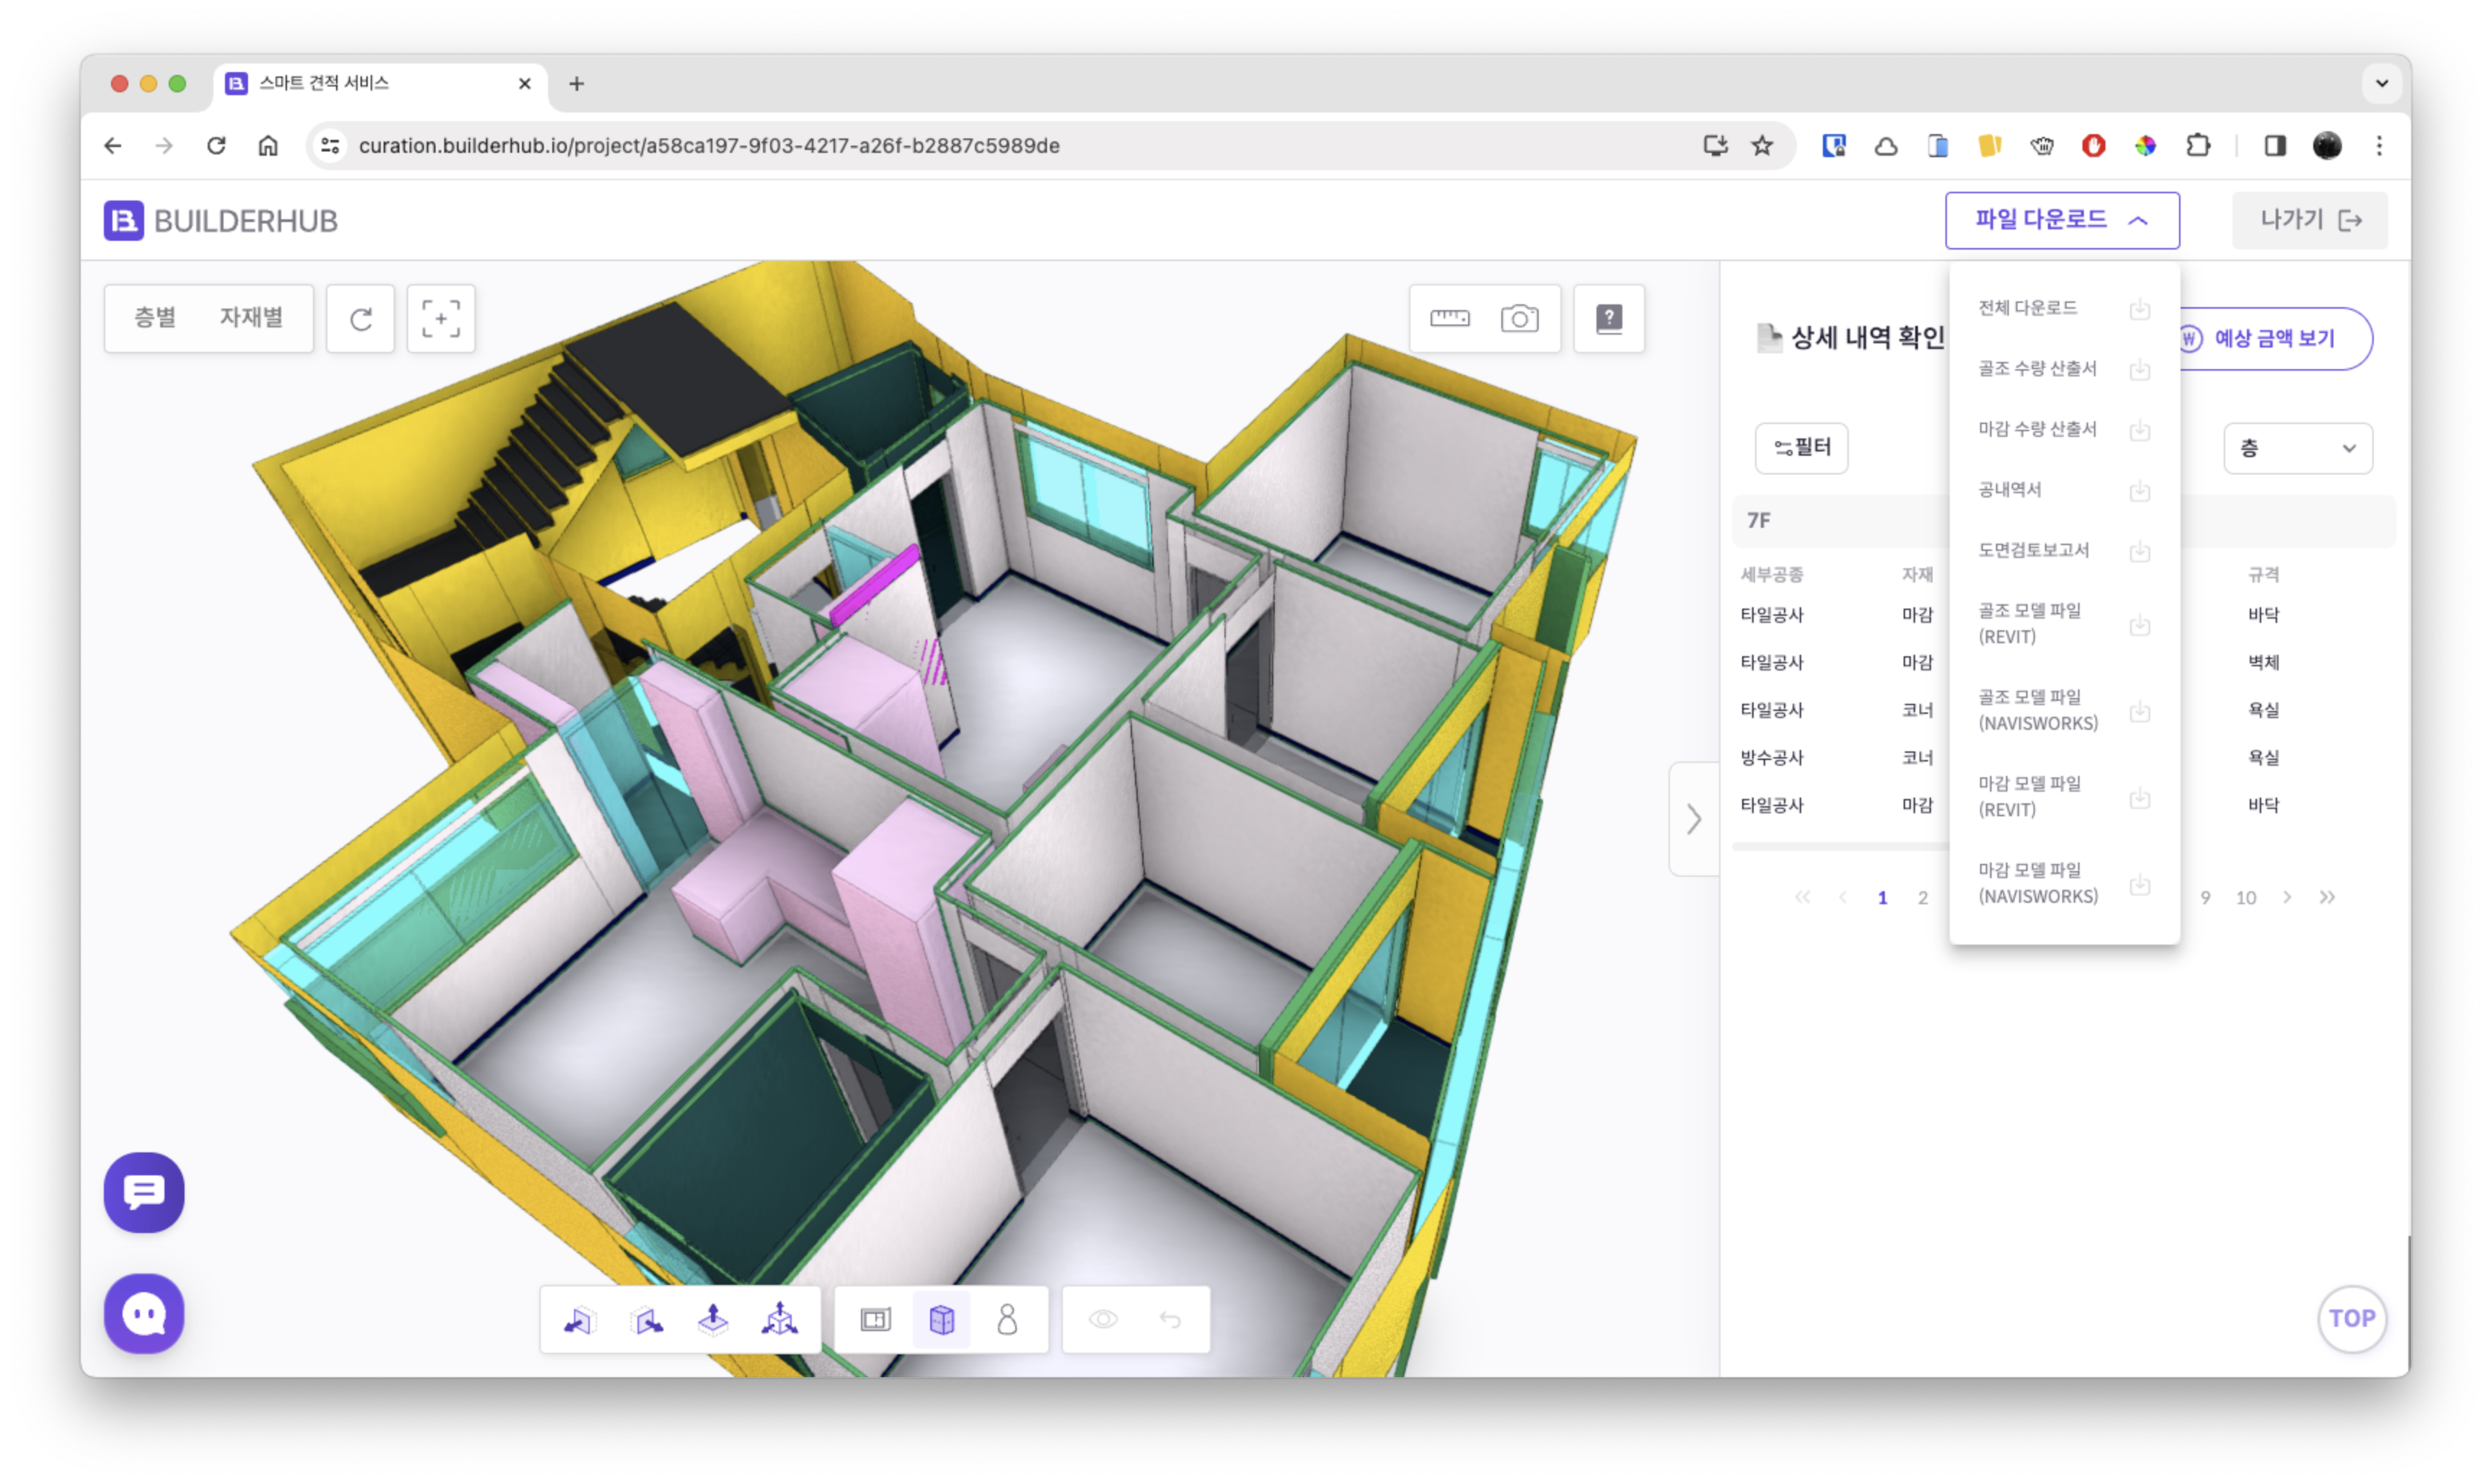
\includegraphics[width=0.35\textwidth]{images/builderhub-curation-download.png}
				      \caption*{Download assets}
			      }\qquad
			      \parbox{0.35\textwidth}{
				      \centering
				      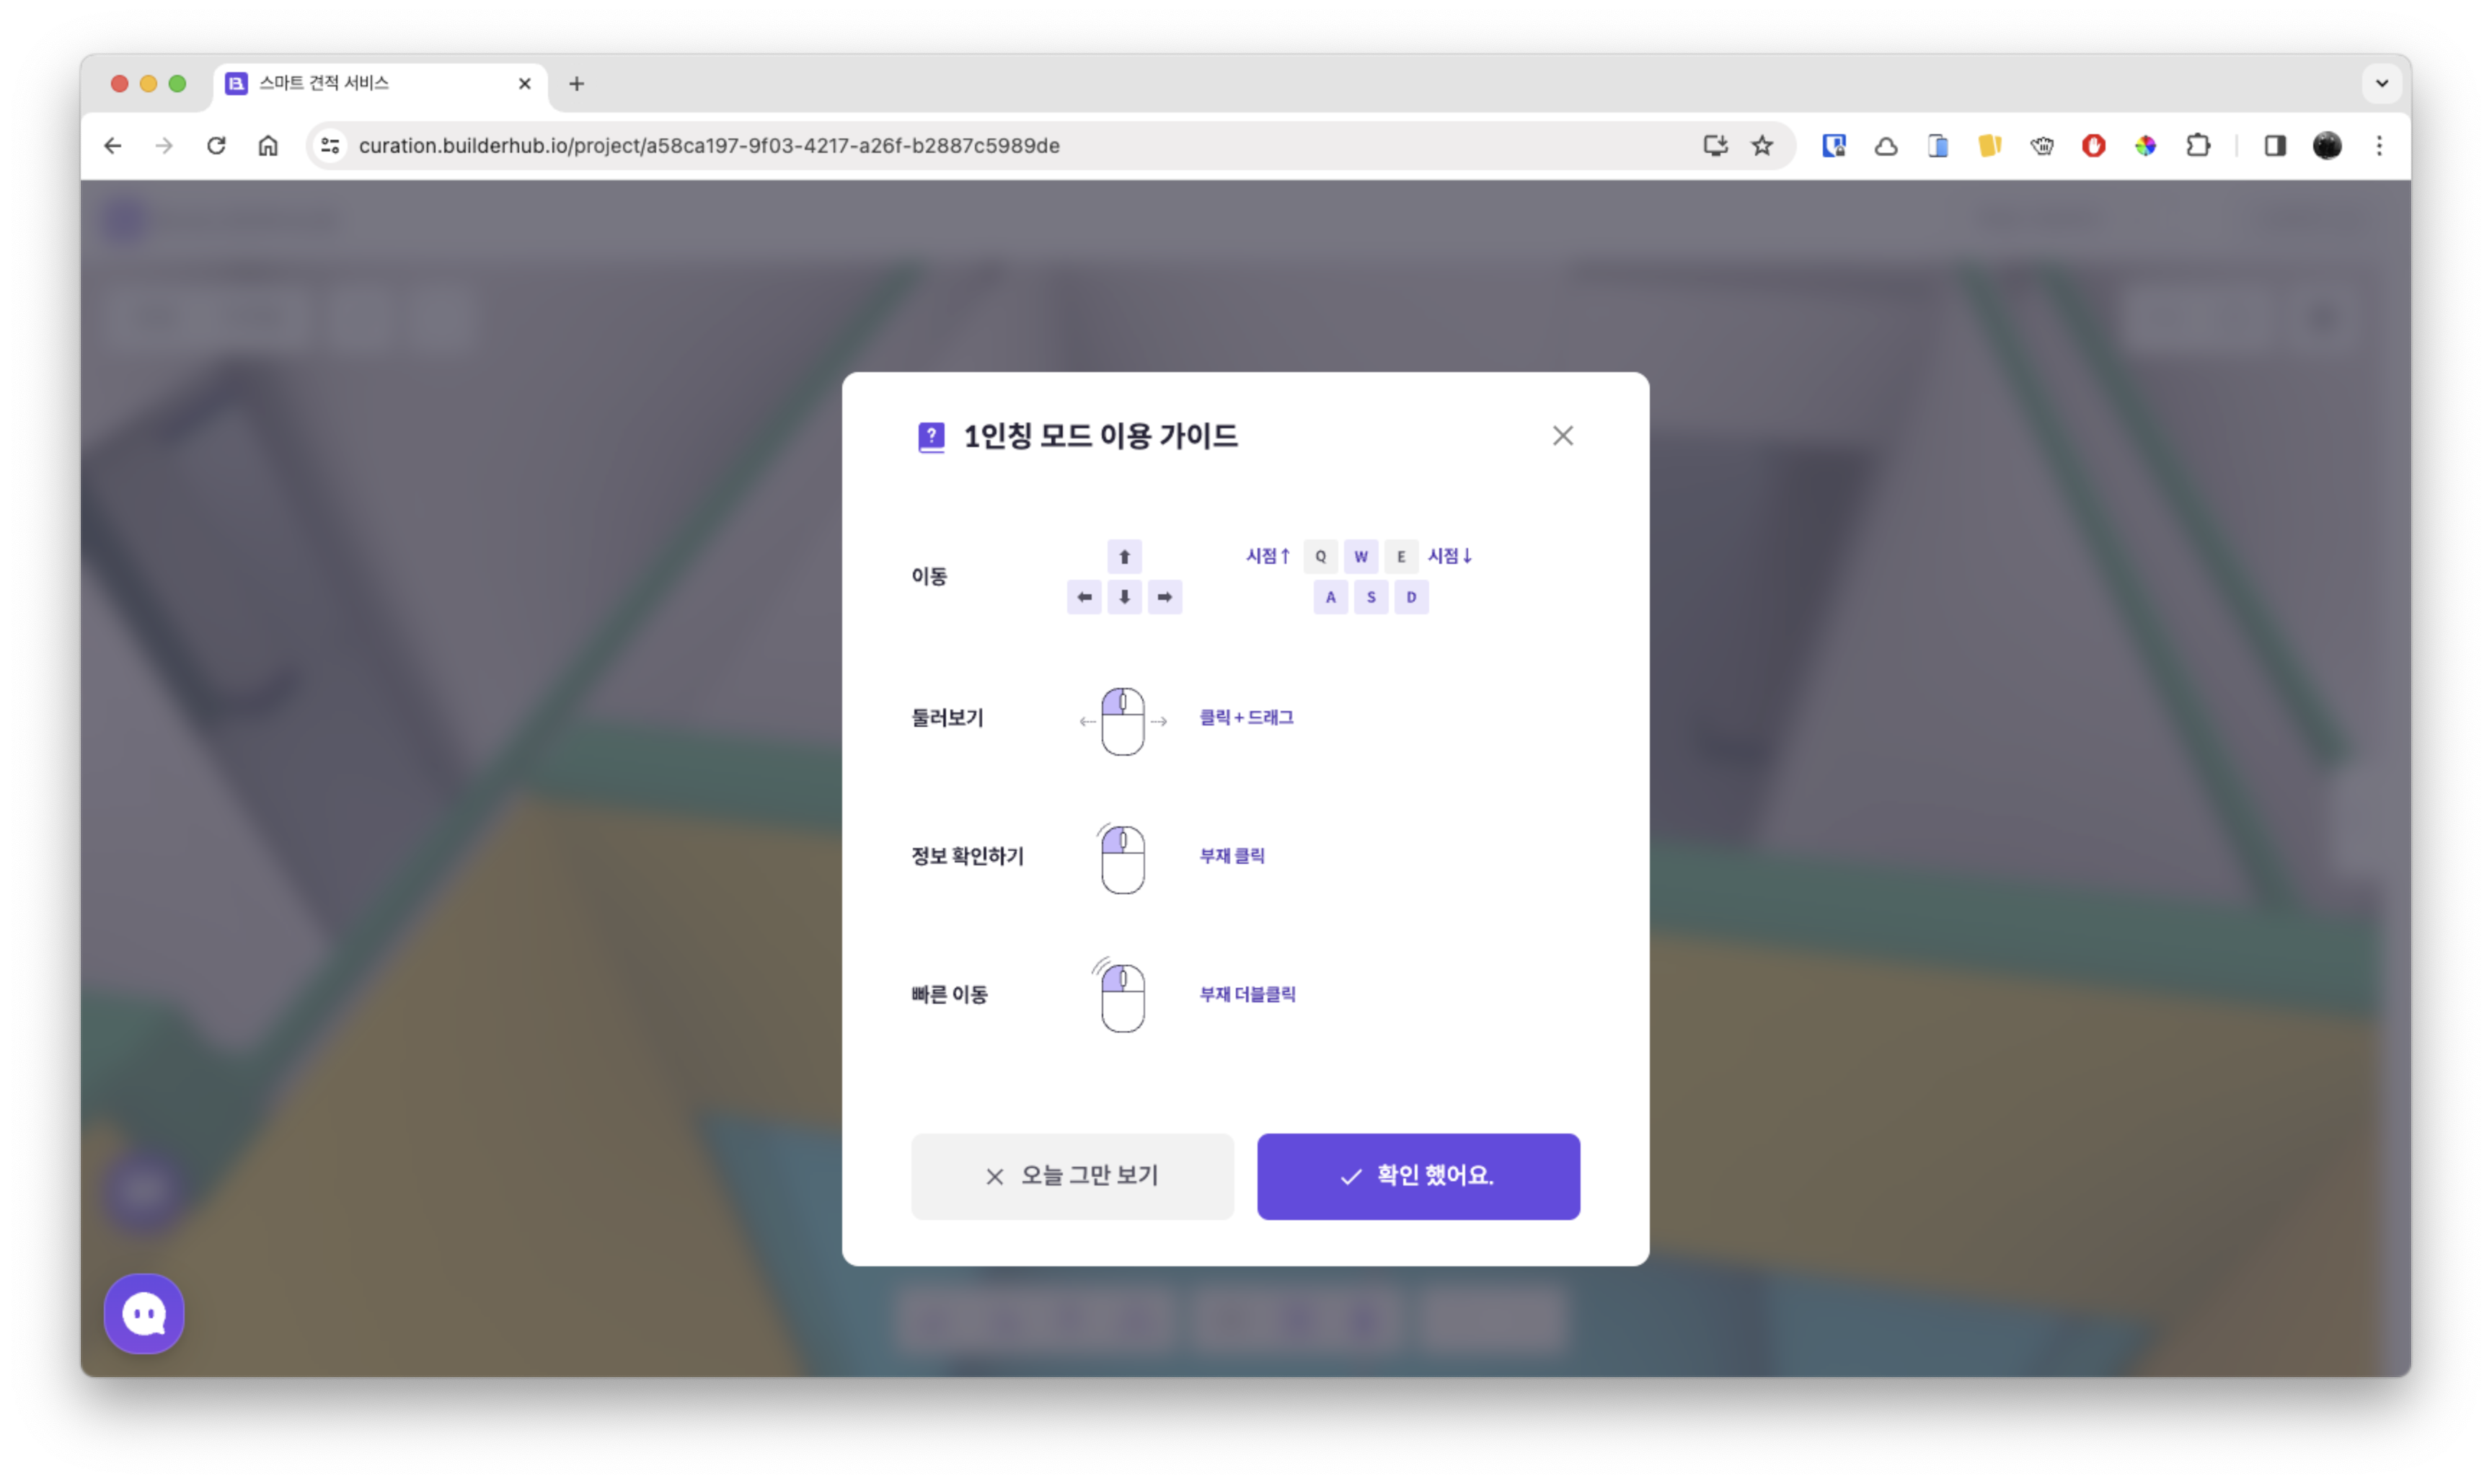
\includegraphics[width=0.35\textwidth]{images/builderhub-curation-first-person-view-1.png}
				      \caption*{First-person view guide}
			      }\qquad
			      \parbox{0.35\textwidth}{
				      \centering
				      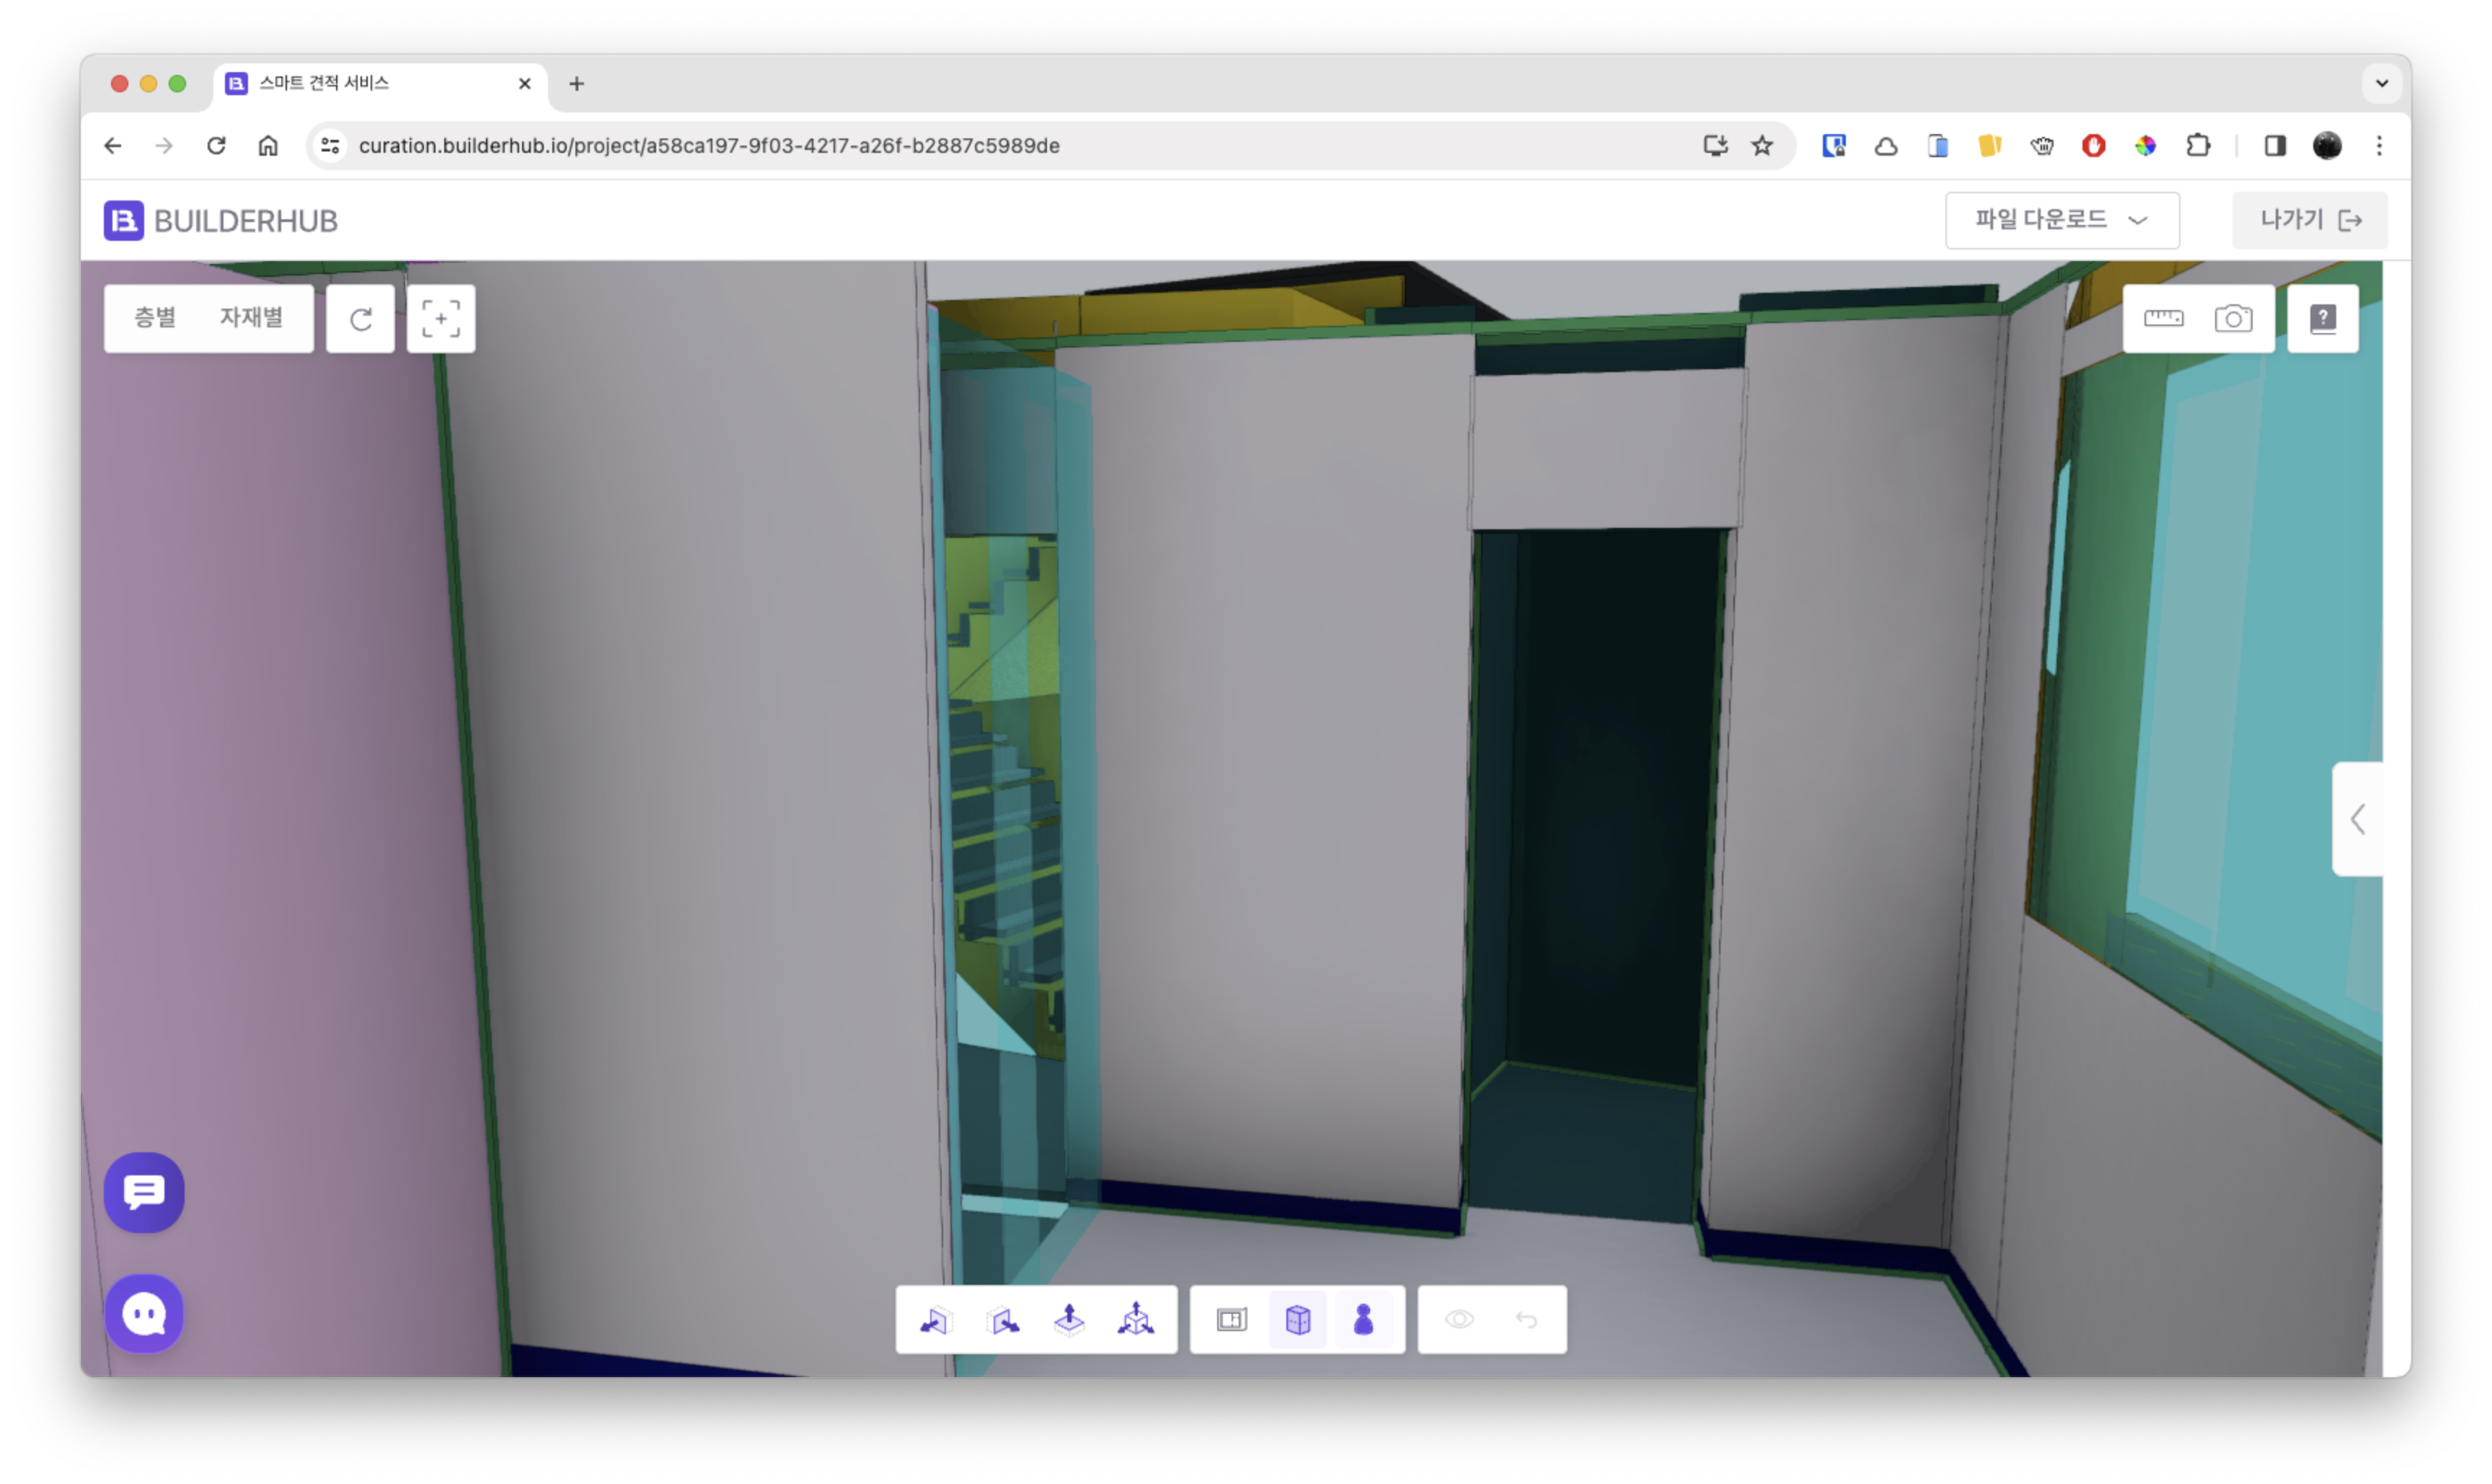
\includegraphics[width=0.35\textwidth]{images/builderhub-curation-first-person-view-2.png}
				      \caption*{Frist-person view control}
			      }\qquad
			      \parbox{0.35\textwidth}{
				      \centering
				      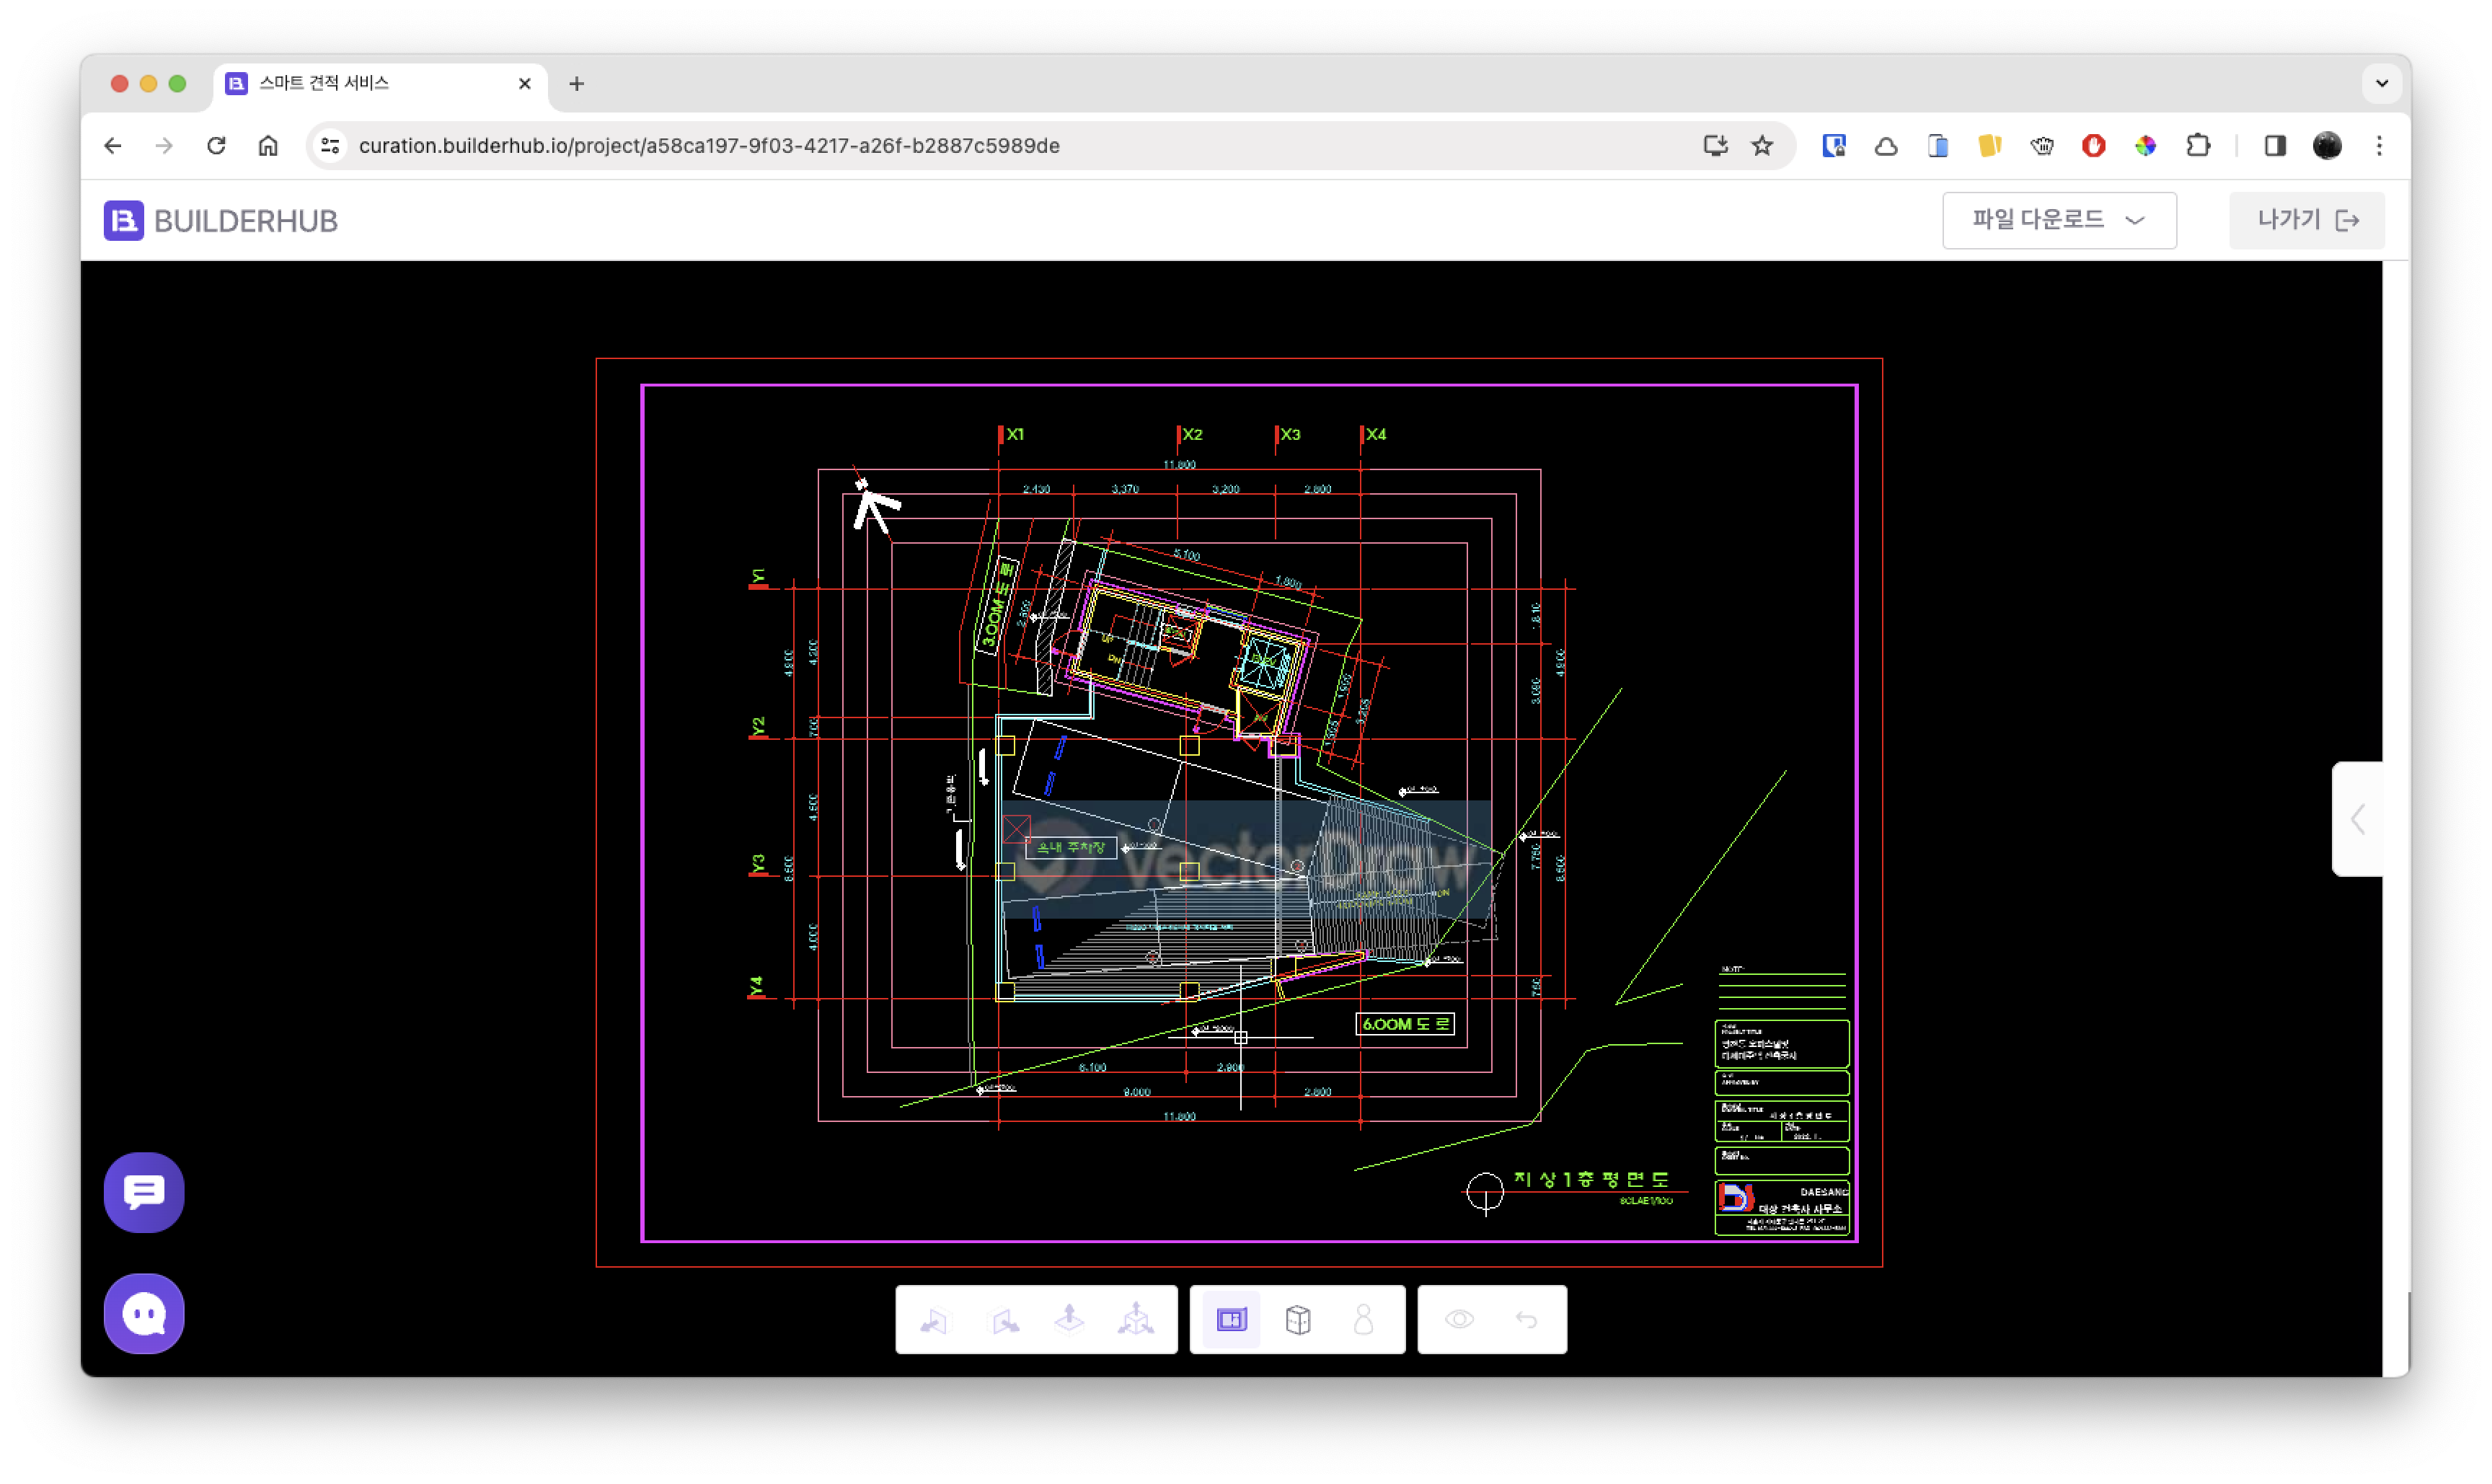
\includegraphics[width=0.35\textwidth]{images/builderhub-curation-2d-view.png}
				      \caption*{2D drawing view}
			      }
		      \end{fullwidth}
	      \end{figure}
	\item \href{https://partners.builderhub.io/}{파트너 서비스} 개발(파트너 등록 및 검수, 공공 API 및 공공 데이터 연동 파트너 정보 등록, 포트폴리오 등록, 블로그 및 콘텐츠 서비스)
	      \begin{itemize}
		      \item 파트너 등록 및 검수, 대시보드, 프로필 수정
		      \item 공공 API 및 공공 데이터 연동 파트너 정보 등록, 포트폴리오 등록, 블로그 및 콘텐츠 서비스 (개발중)
	      \end{itemize}
	      \begin{figure}[!ht]
		      \begin{fullwidth}
			      \parbox{0.35\textwidth}{
				      \centering
				      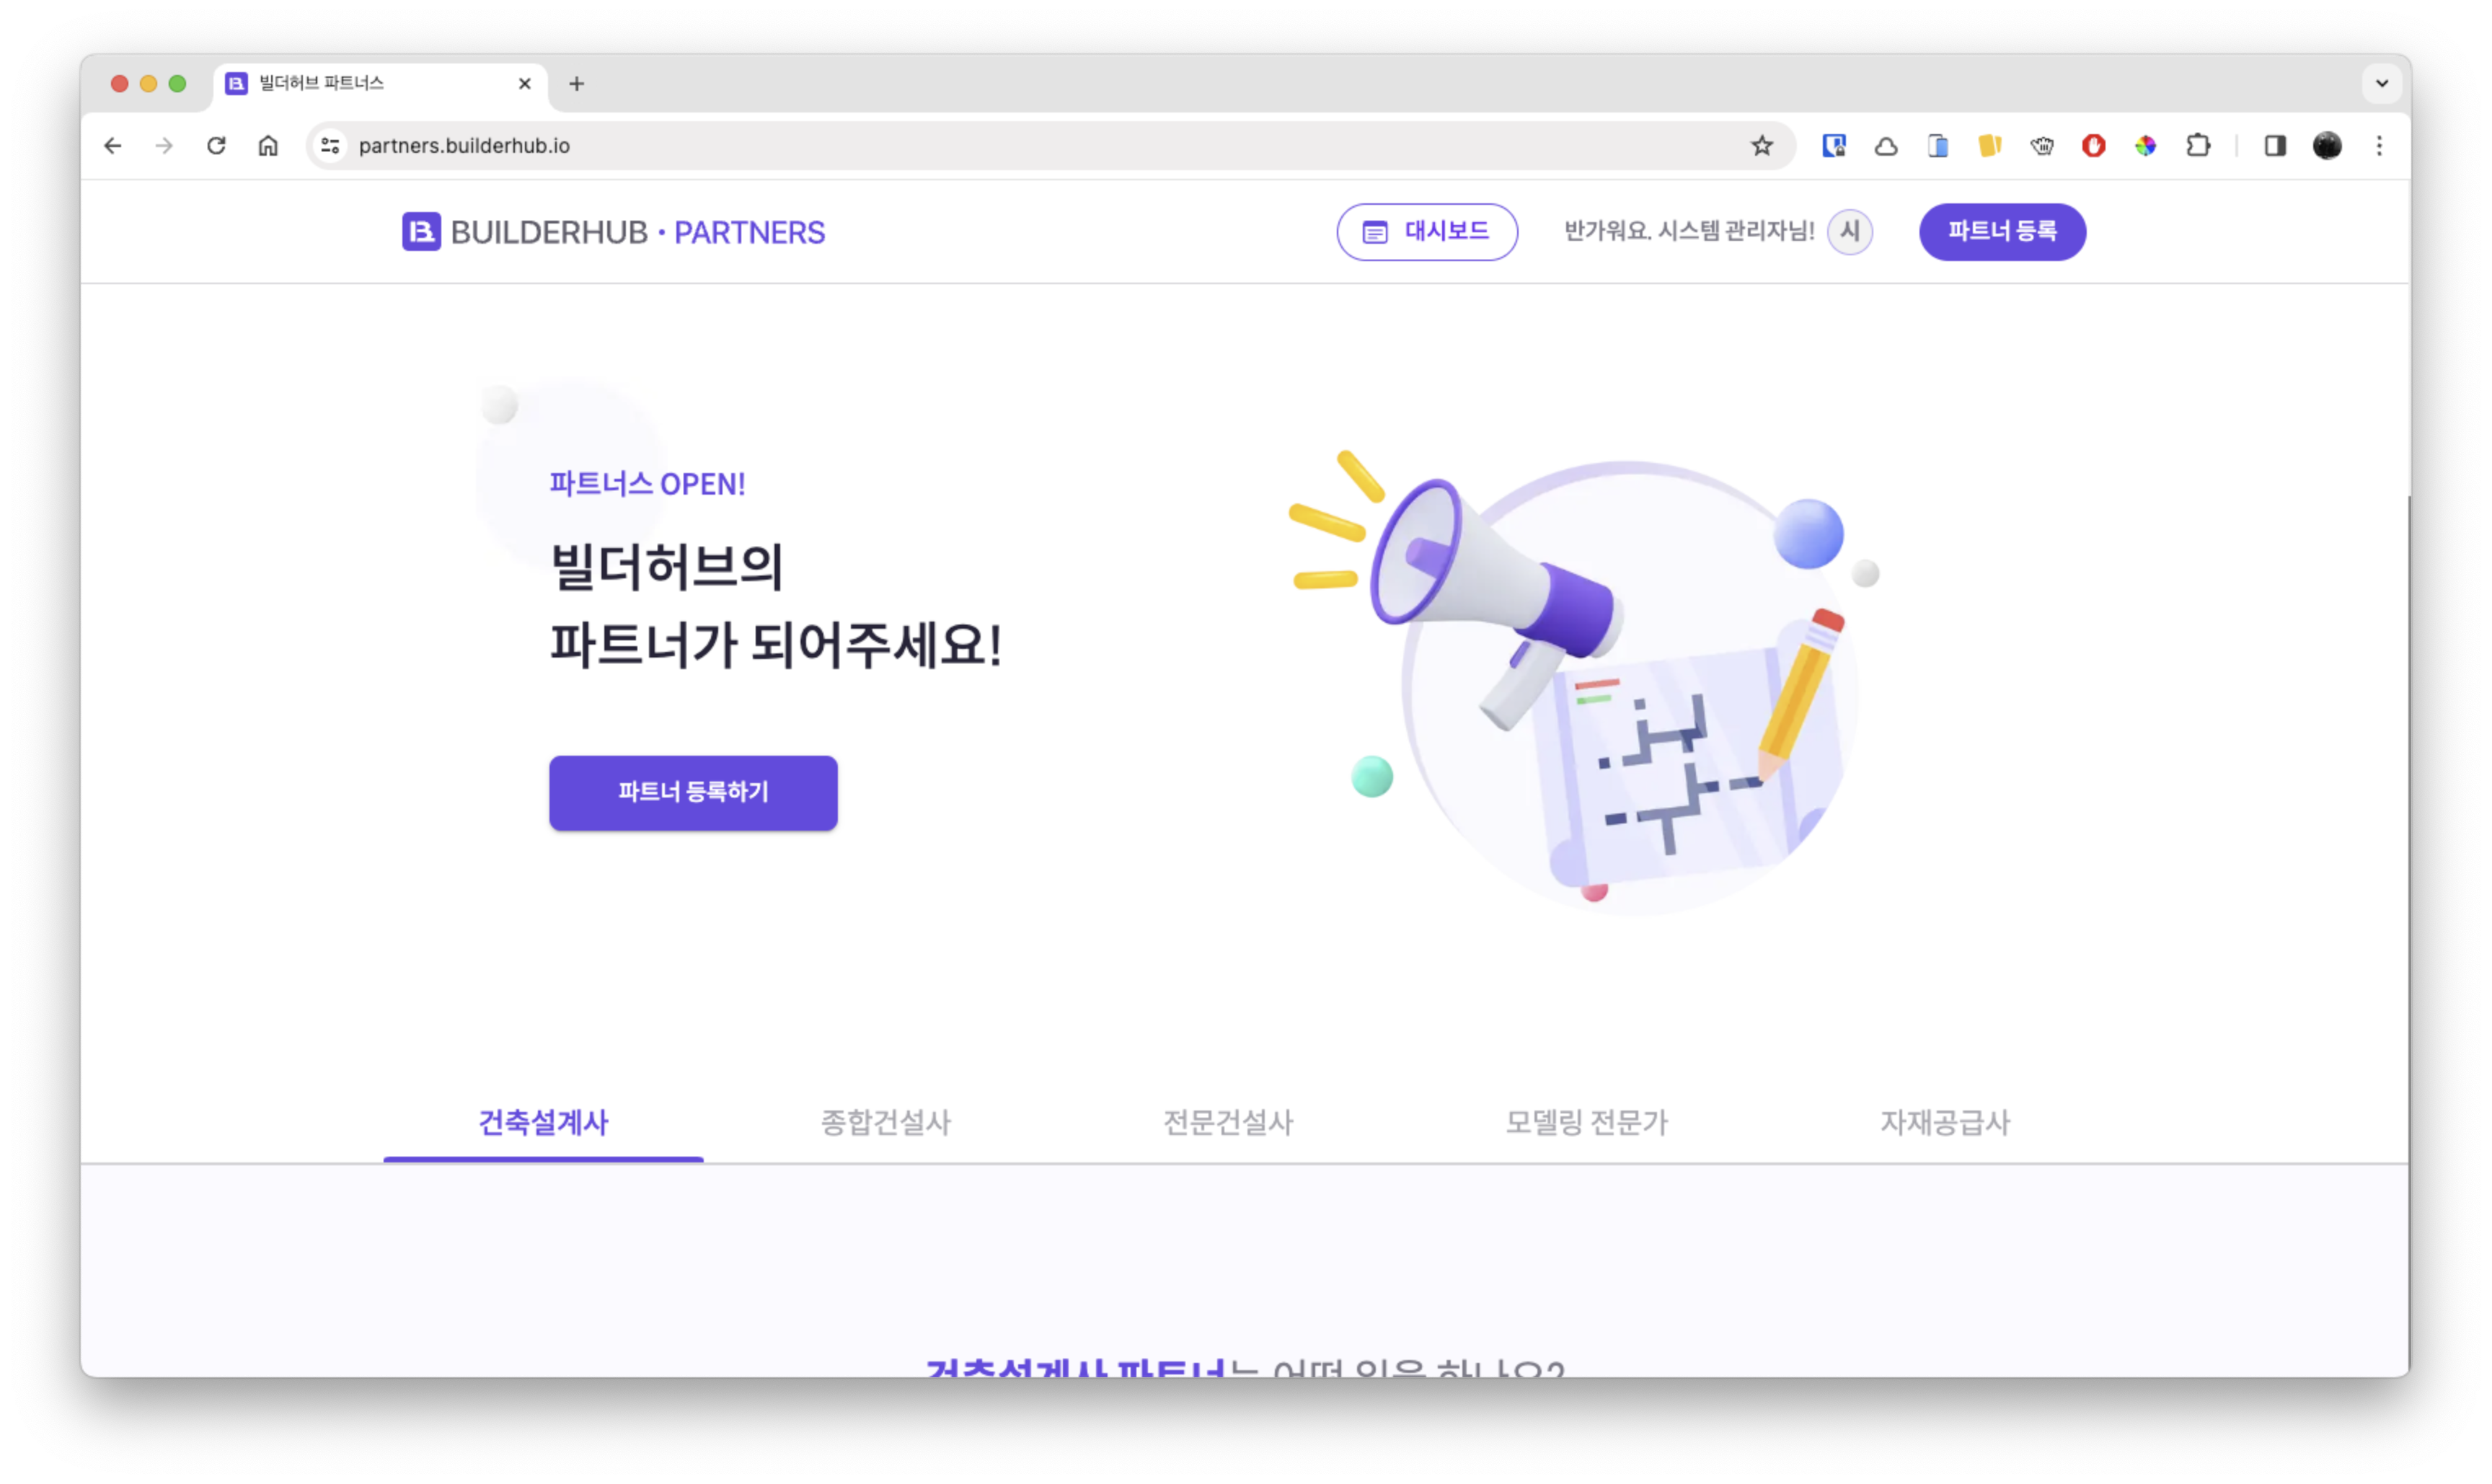
\includegraphics[width=0.35\textwidth]{images/builderhub-partners-main.png}
				      \caption*{Landing page}
			      }\qquad
			      \parbox{0.35\textwidth}{
				      \centering
				      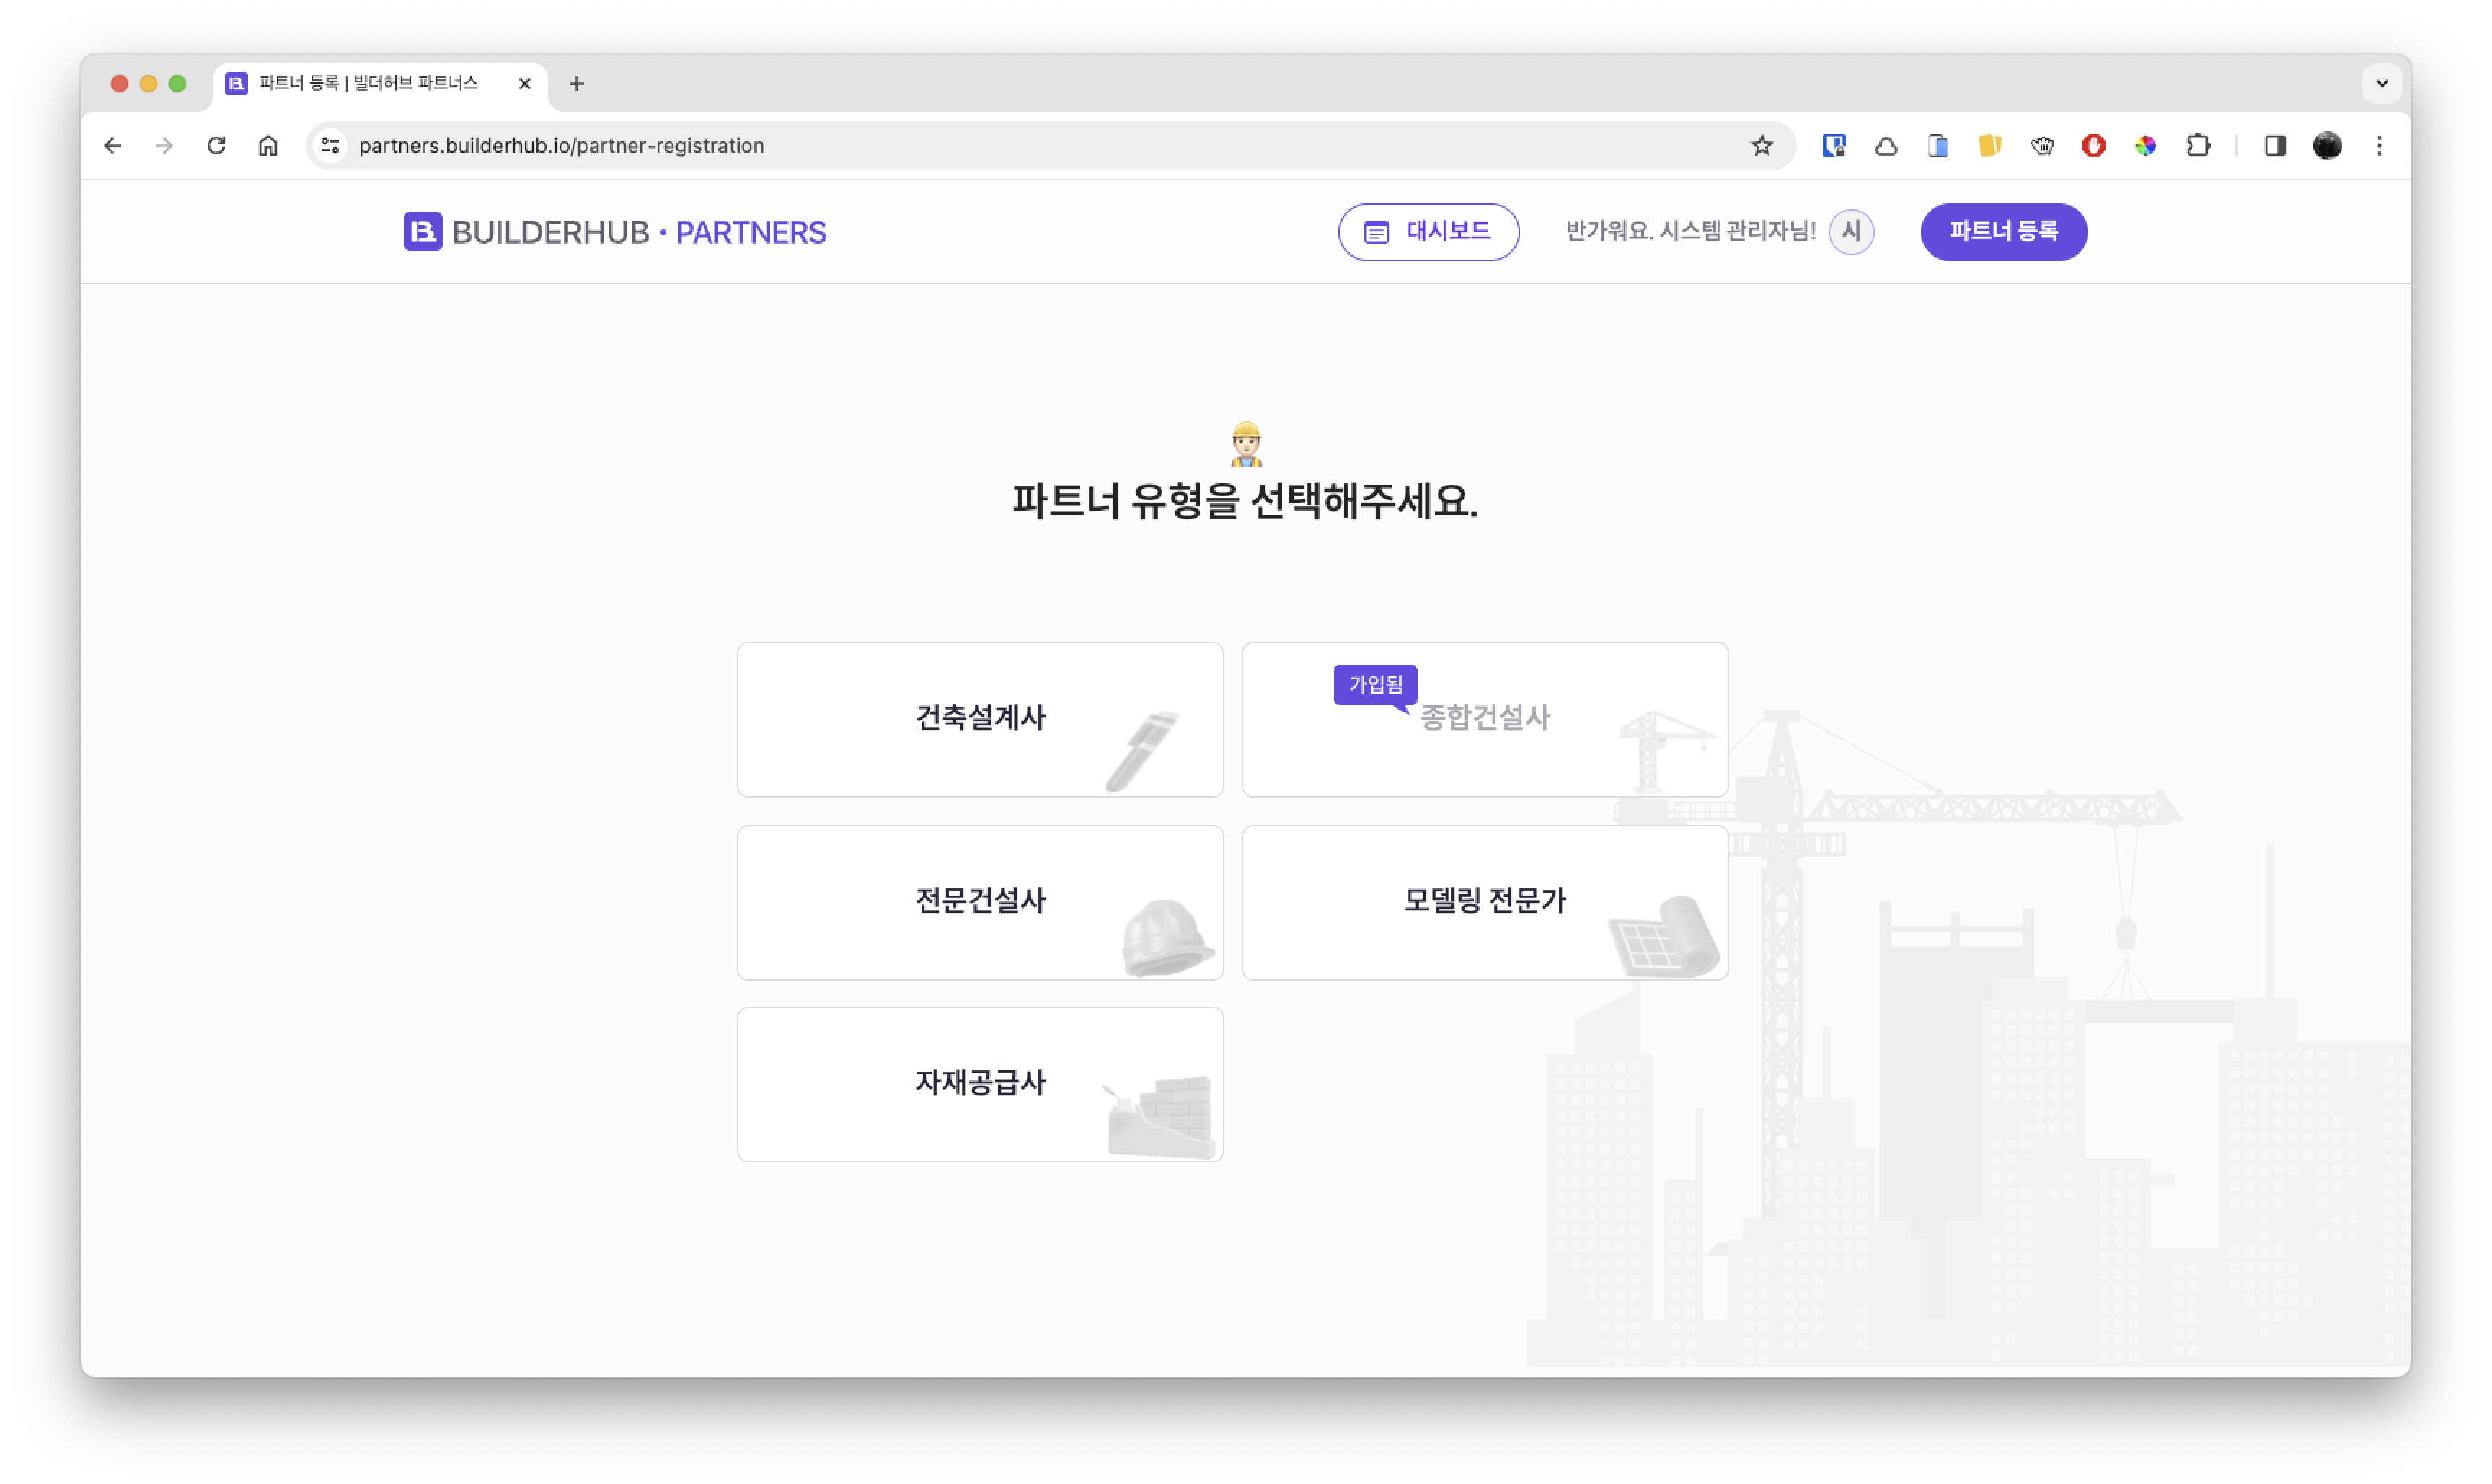
\includegraphics[width=0.35\textwidth]{images/builderhub-partners-join.png}
				      \caption*{Join partner}
			      }\qquad
			      \parbox{0.35\textwidth}{
				      \centering
				      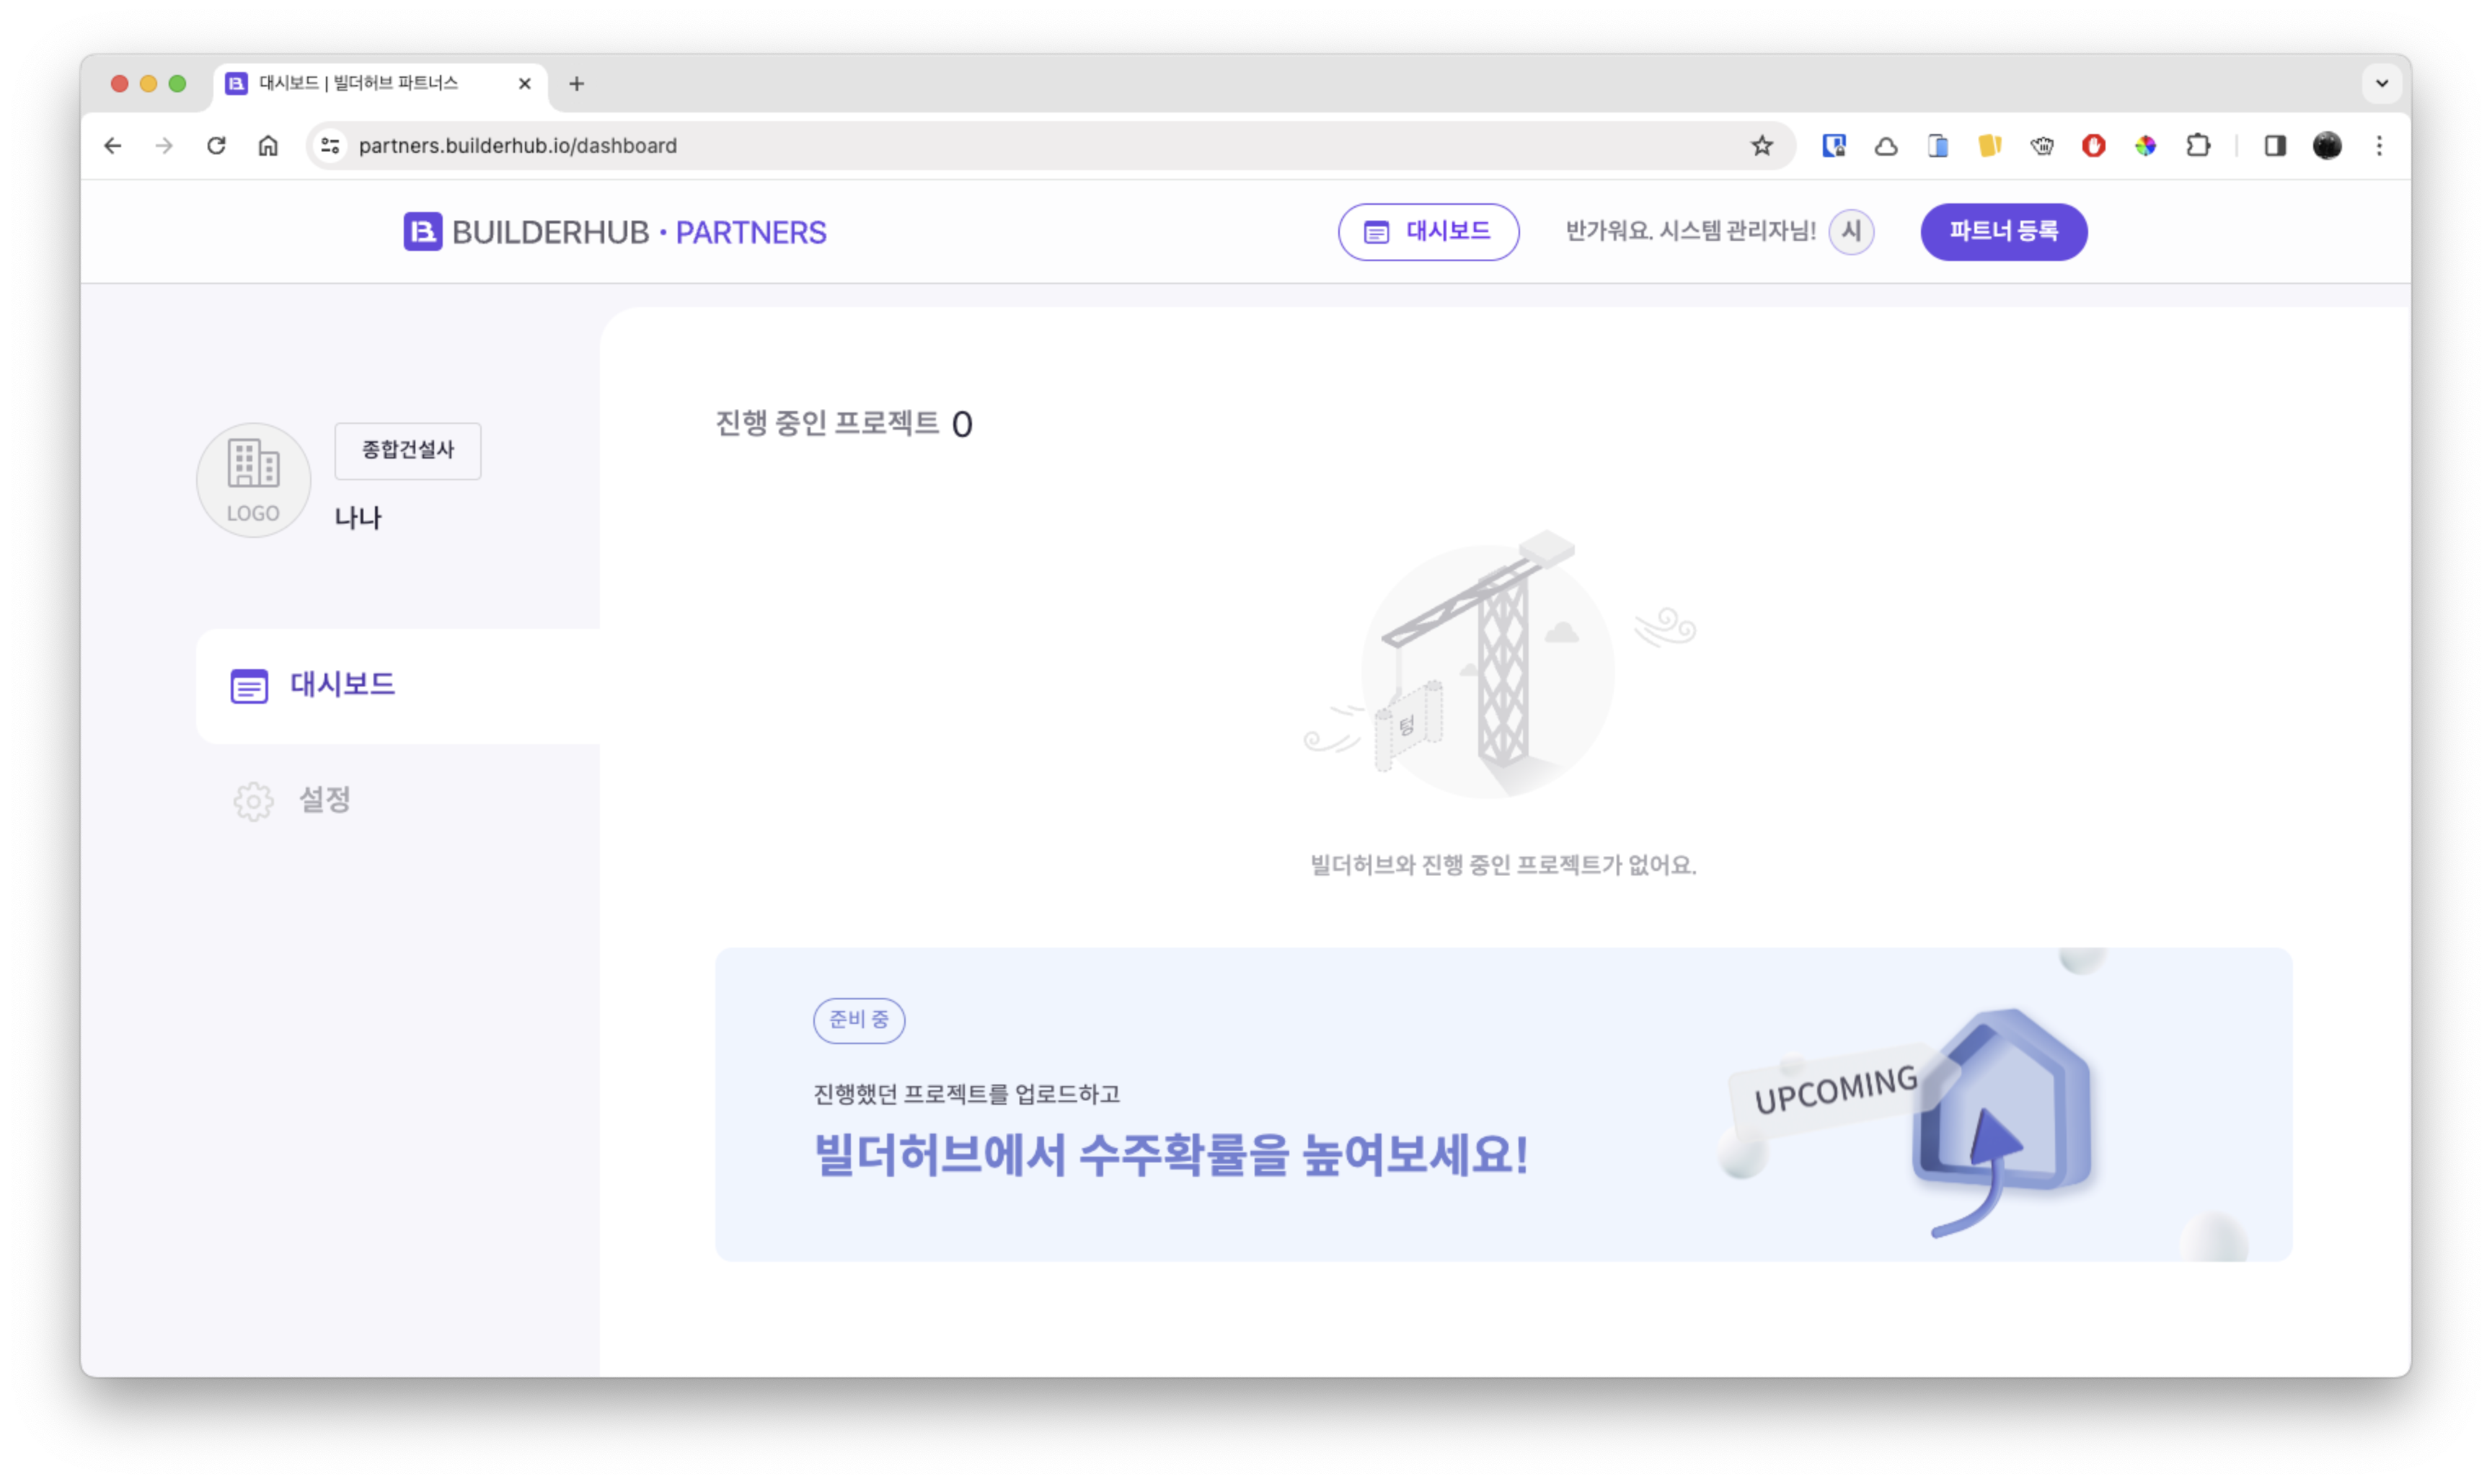
\includegraphics[width=0.35\textwidth]{images/builderhub-partners-dashboard.png}
				      \caption*{Dashboard}
			      }\qquad
			      \parbox{0.35\textwidth}{
				      \centering
				      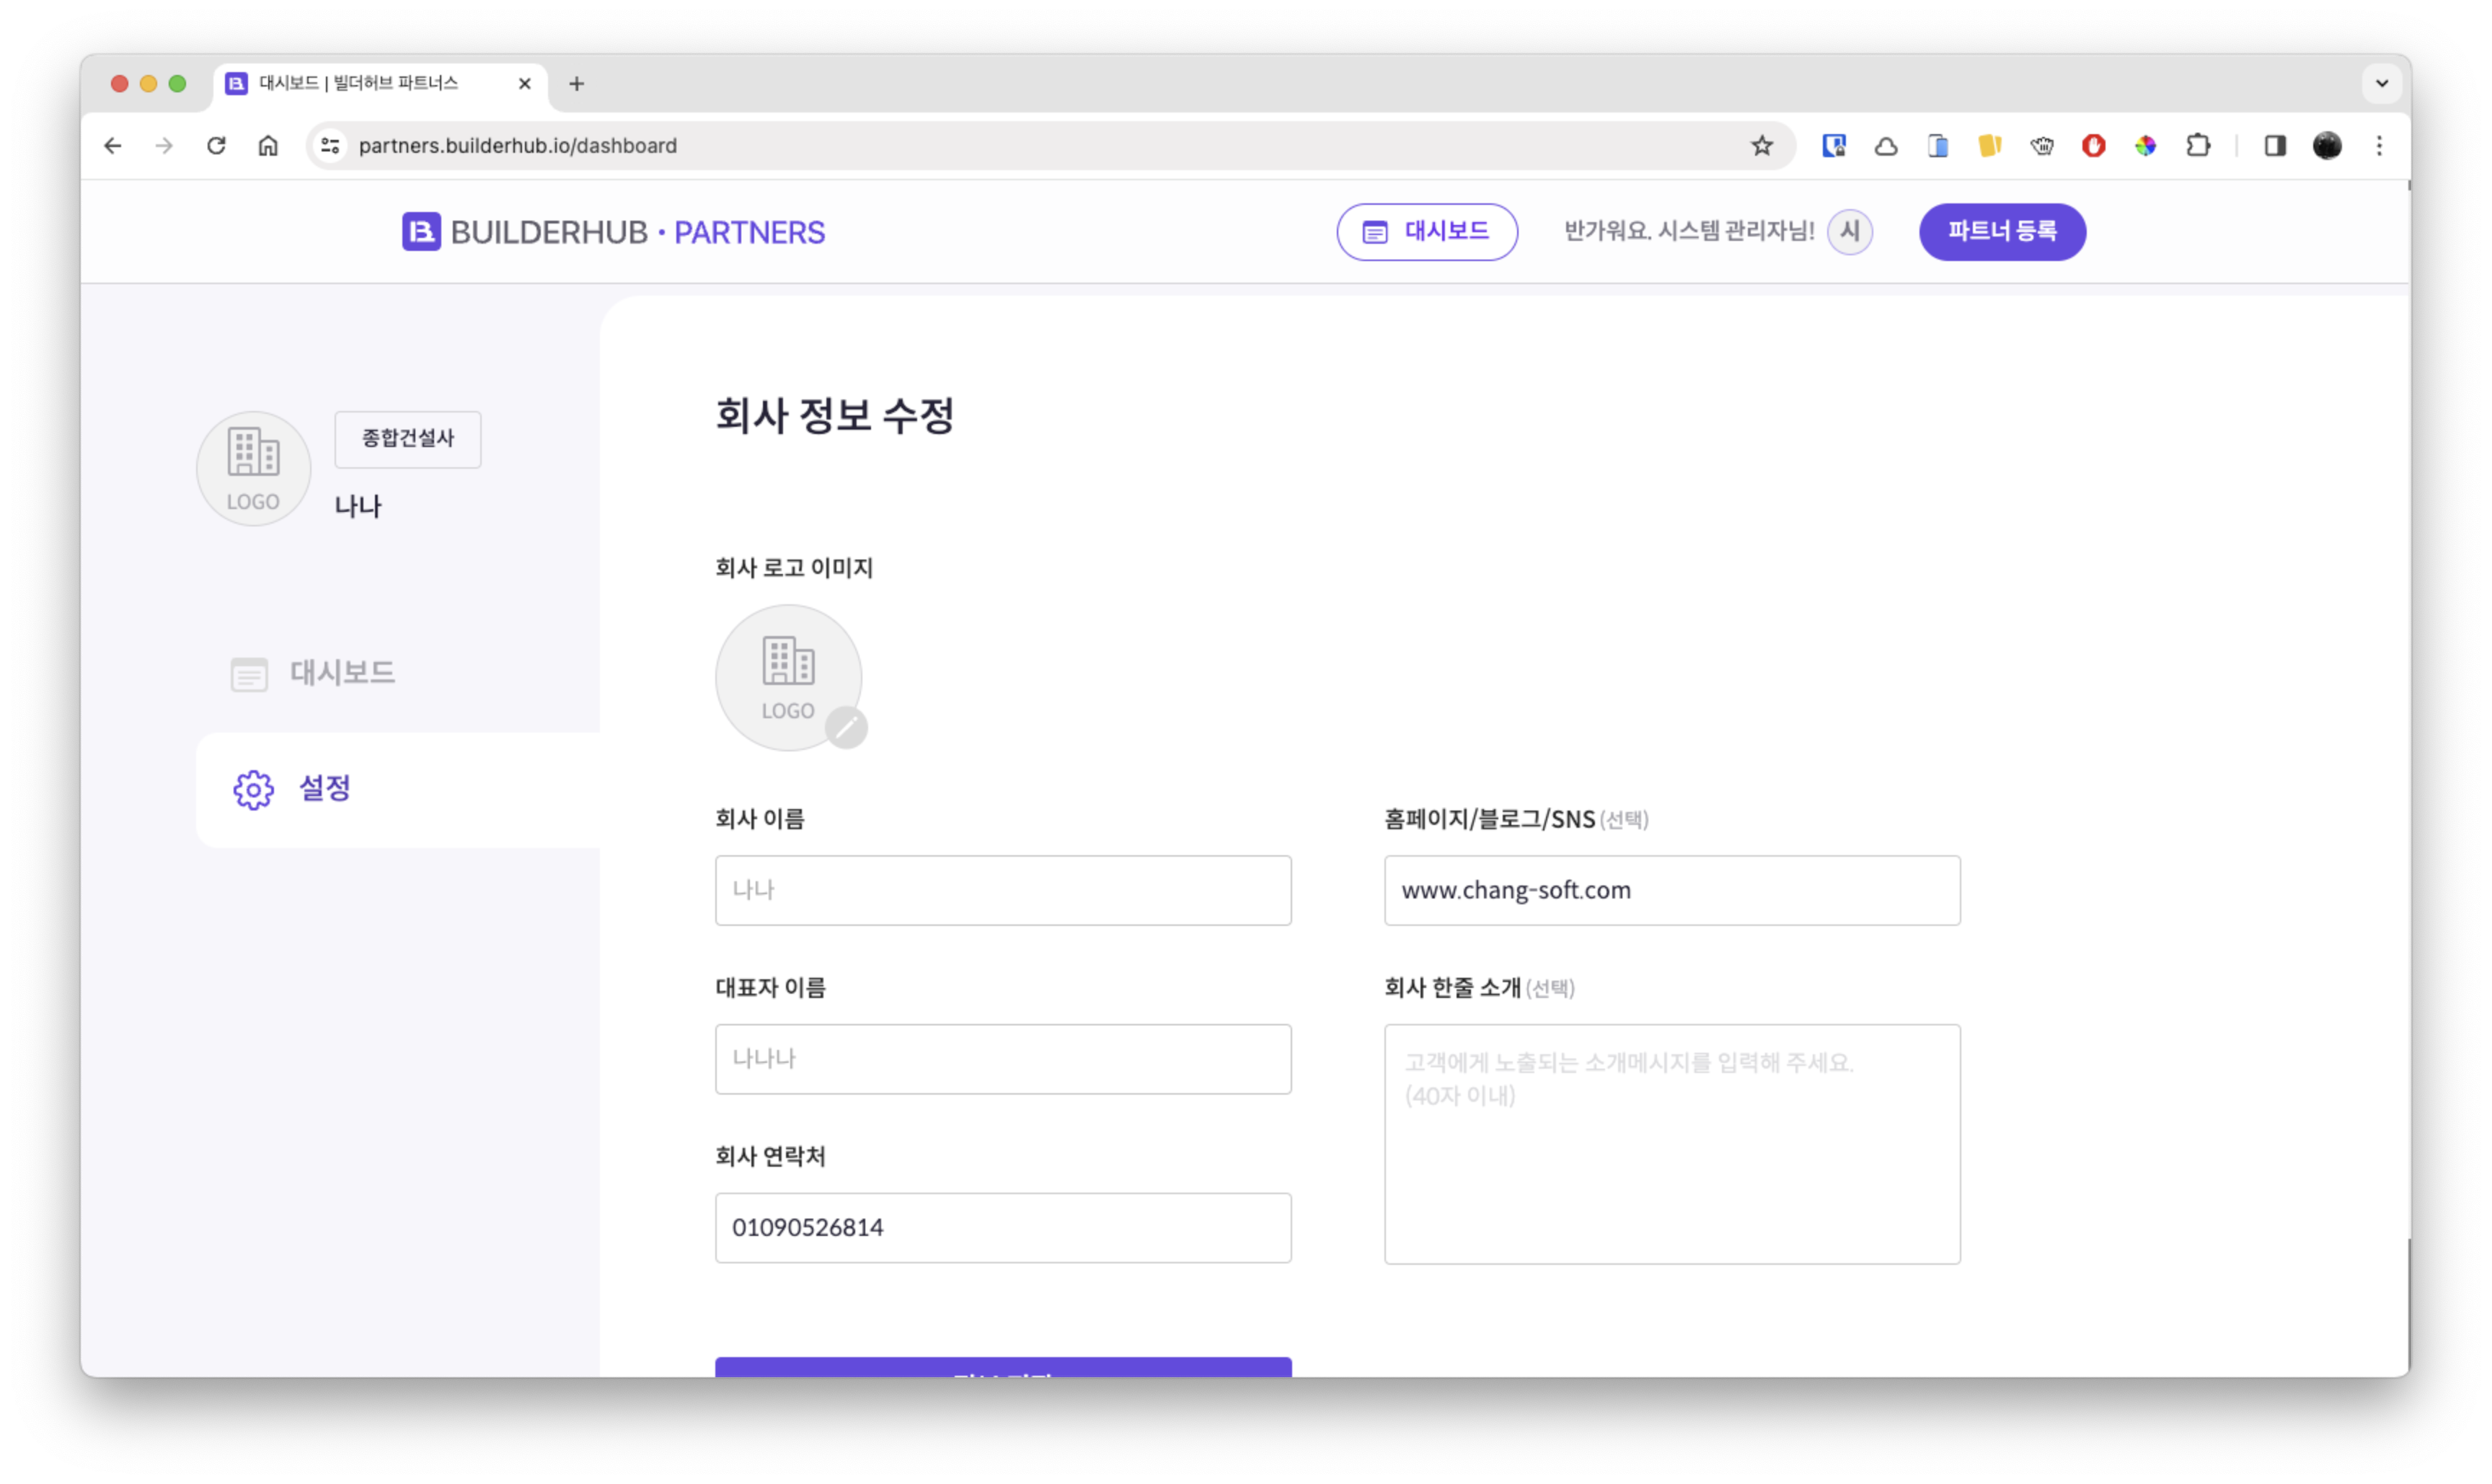
\includegraphics[width=0.35\textwidth]{images/builderhub-partners-edit.png}
				      \caption*{Edit profile}
			      }
		      \end{fullwidth}
	      \end{figure}
	\item \href{https://admin.prod.platform.builderhub.io/}{빌더허브 운영 어드민 (Back office)} 개발(프로젝트 검수, 파트너 검수, 알림톡 송출, 결제 확인, 프로젝트 에셋 등록, 표준내역서 관리, 1:1문의 답변, FAQ 작성 등)
	      \begin{itemize}
		      \item 프로젝트 검수, 파트너 검수, 알림톡 송출, 결제 확인
		      \item 프로젝트 에셋 등록, 표준내역서 관리, 1:1문의 답변, FAQ 작성
	      \end{itemize}
	      \begin{figure}[!ht]
		      \begin{fullwidth}
			      \parbox{0.35\textwidth}{
				      \centering
				      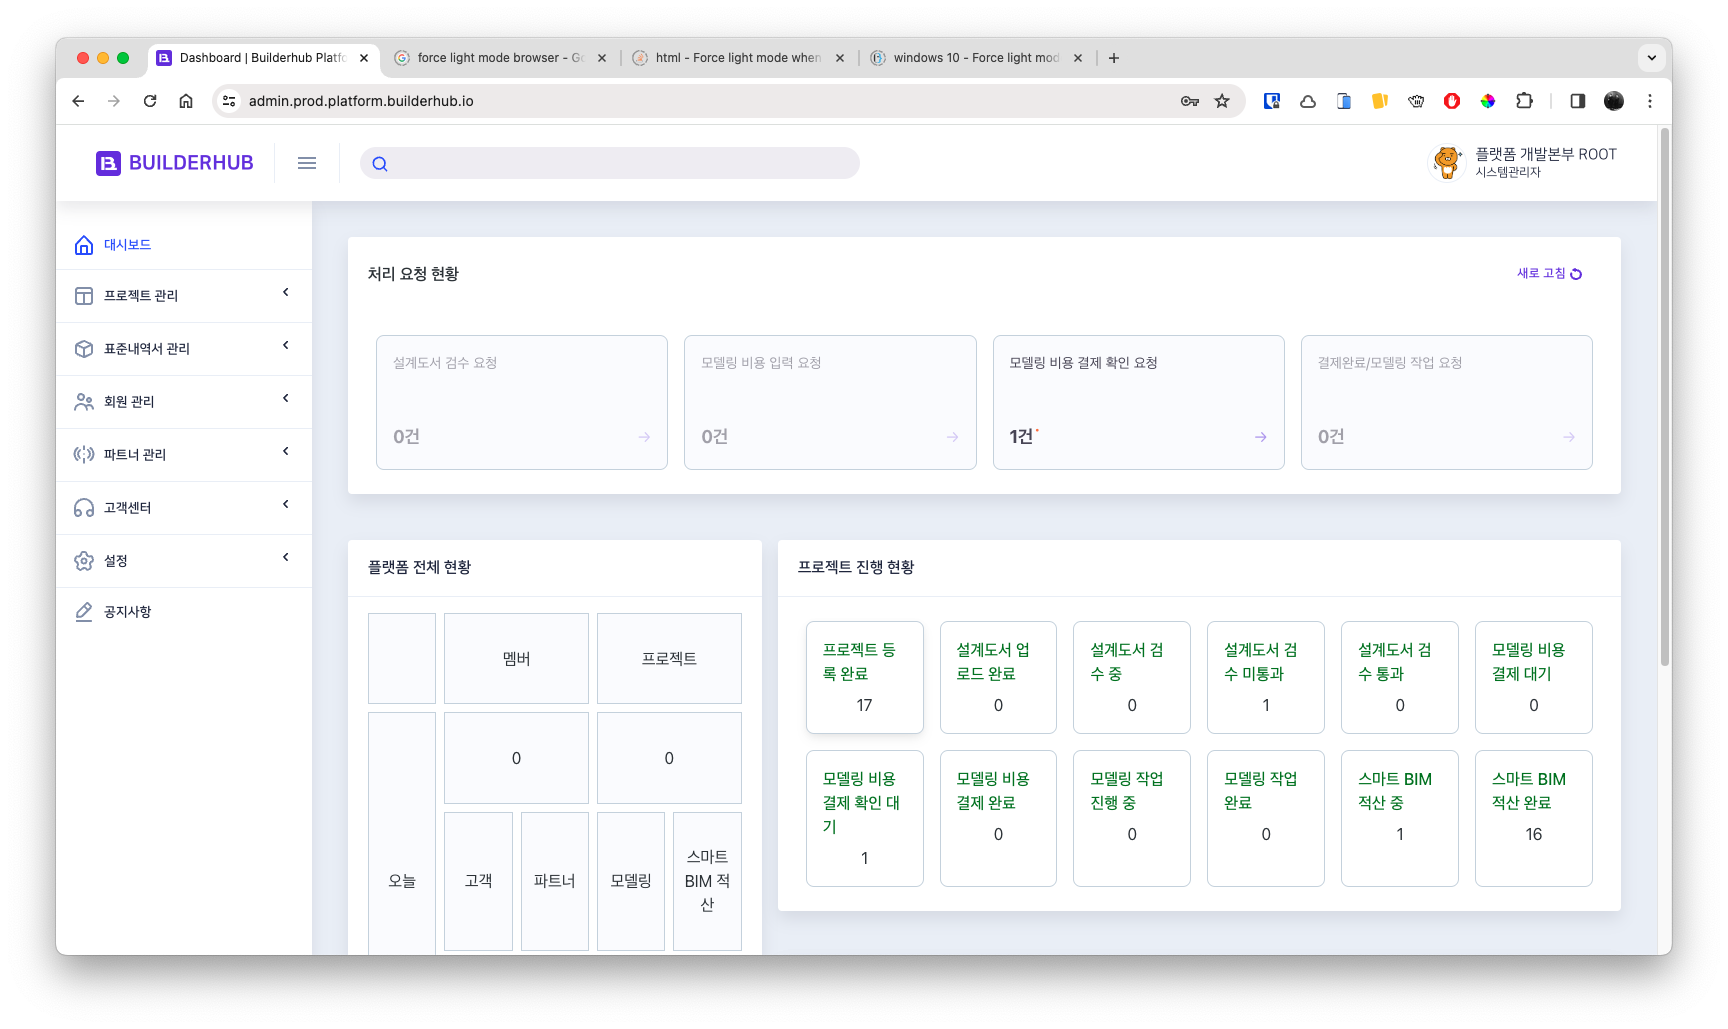
\includegraphics[width=0.35\textwidth]{images/builderhub-admin-dashboard.png}
				      \caption*{Dashboard}
			      }\qquad
			      \parbox{0.35\textwidth}{
				      \centering
				      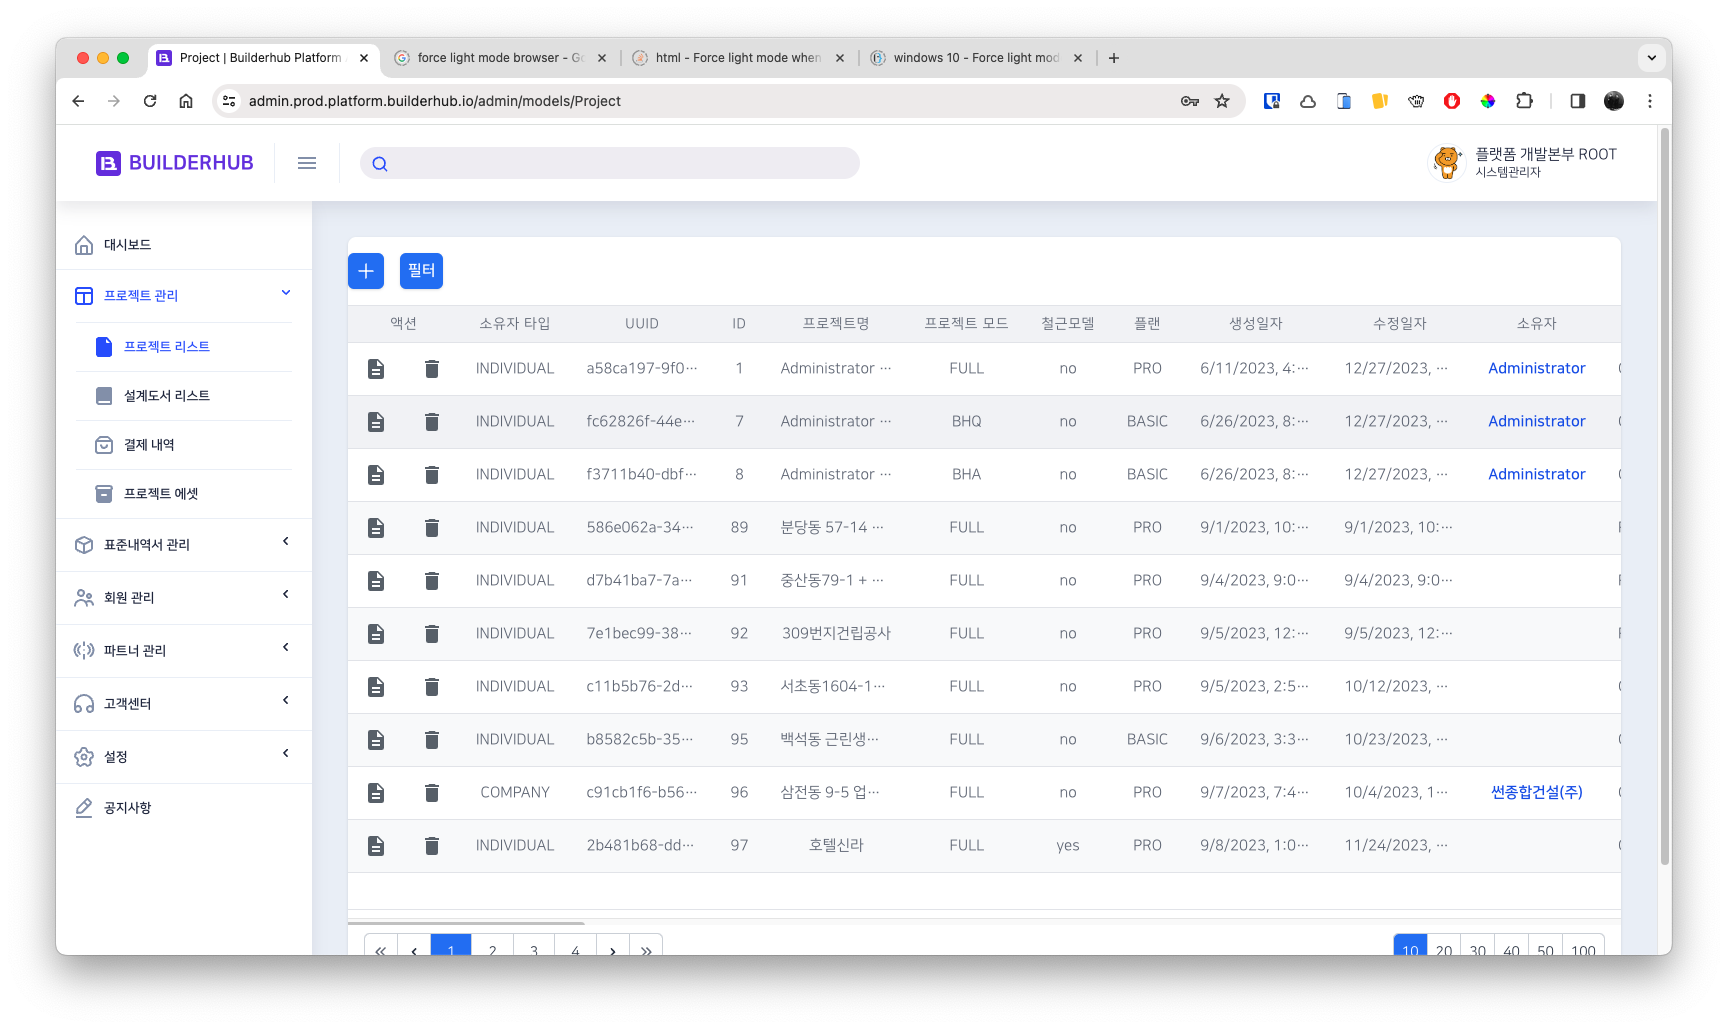
\includegraphics[width=0.35\textwidth]{images/builderhub-admin-project-list.png}
				      \caption*{Project list}
			      }\qquad
			      \parbox{0.35\textwidth}{
				      \centering
				      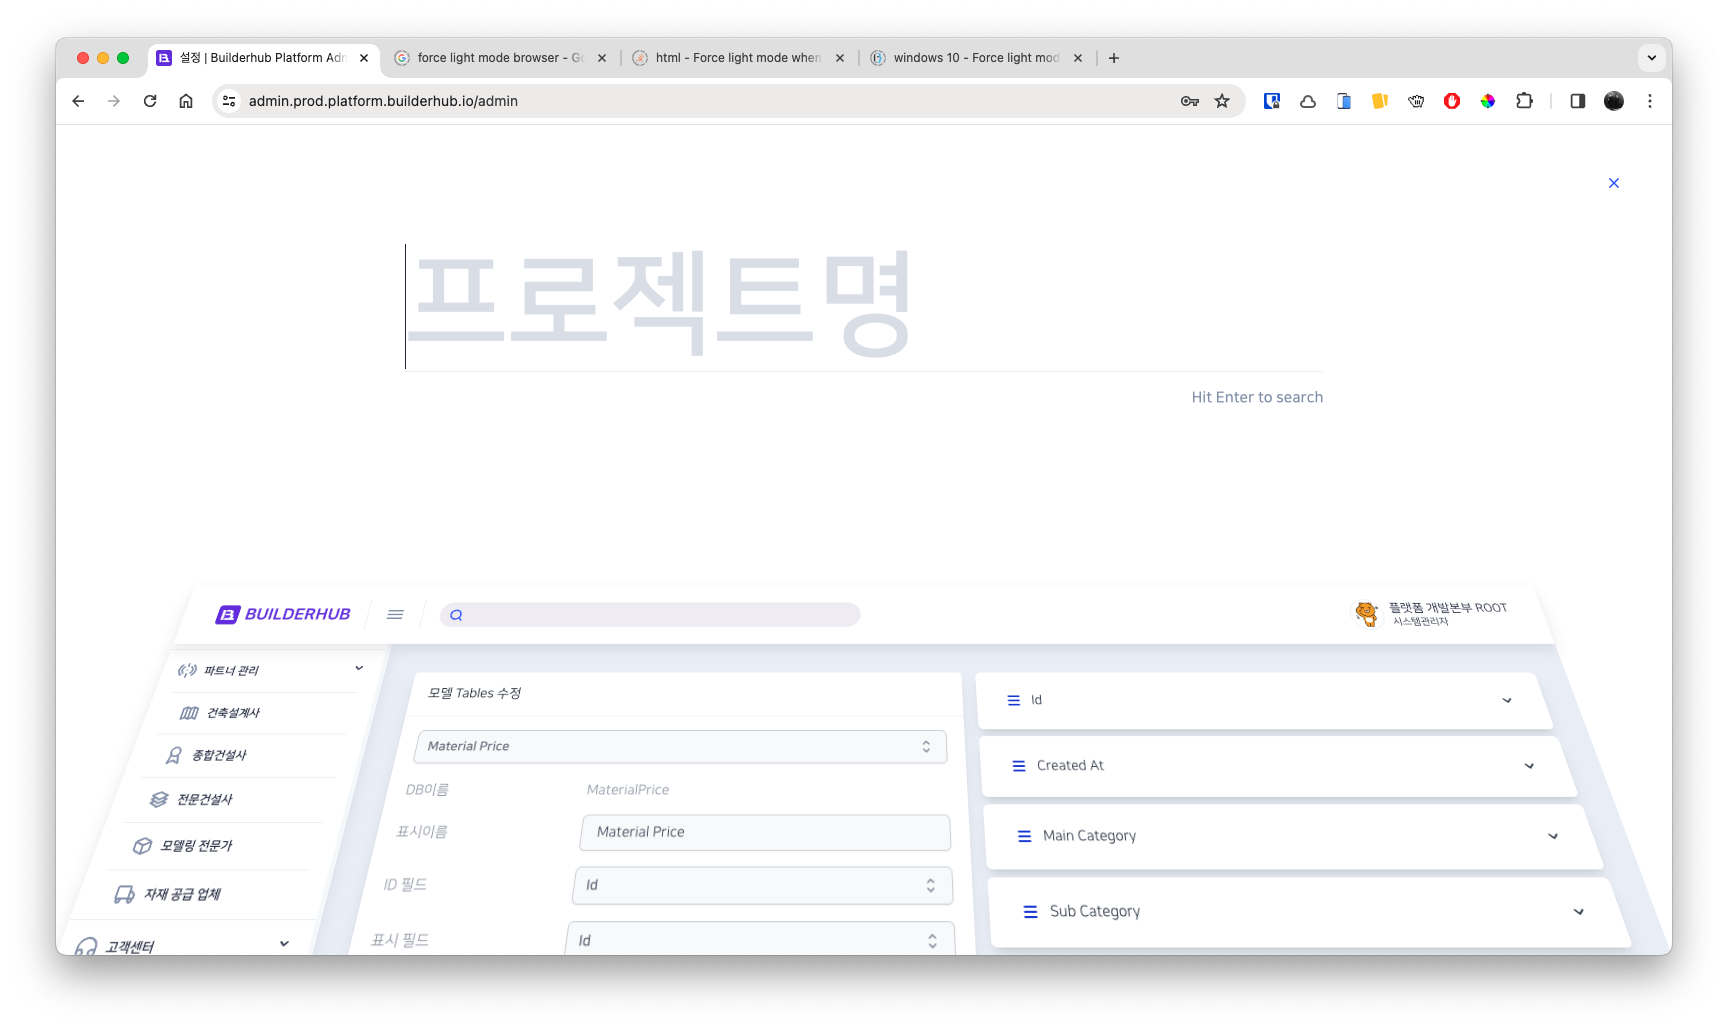
\includegraphics[width=0.35\textwidth]{images/builderhub-admin-project-search.png}
				      \caption*{Project search}
			      }\qquad
			      \parbox{0.35\textwidth}{
				      \centering
				      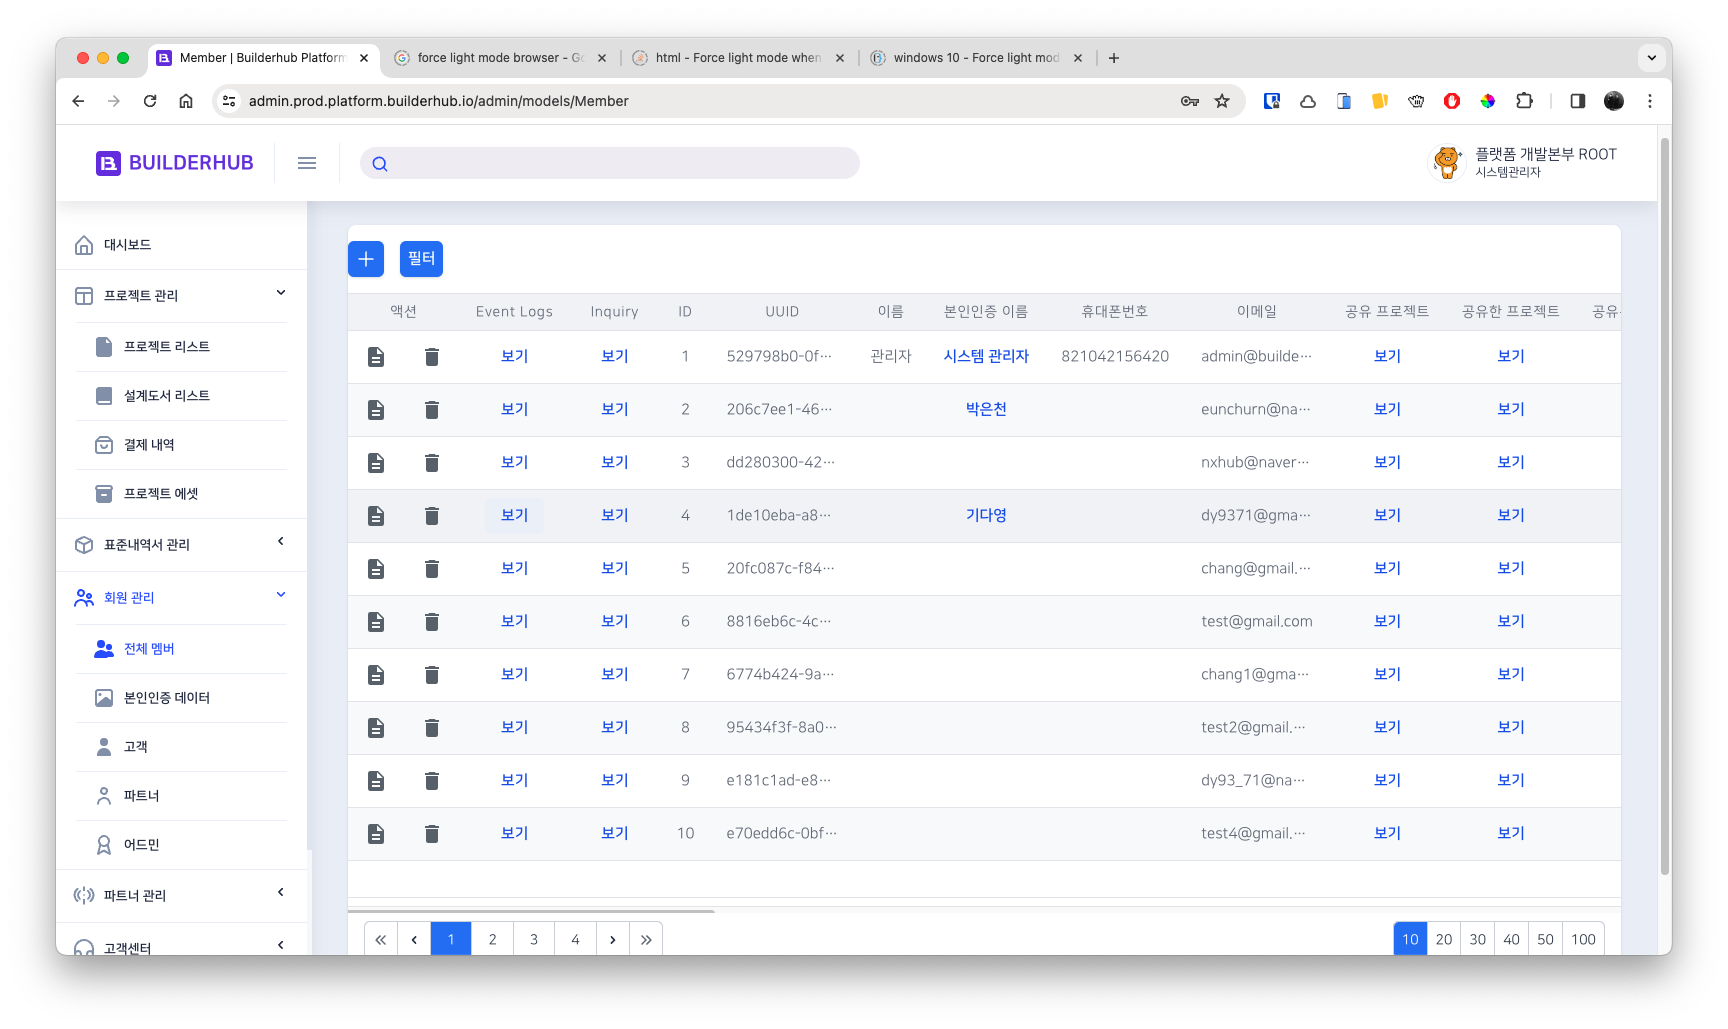
\includegraphics[width=0.35\textwidth]{images/builderhub-admin-member-list.png}
				      \caption*{Member list}
			      }
			      \parbox{0.35\textwidth}{
				      \centering
				      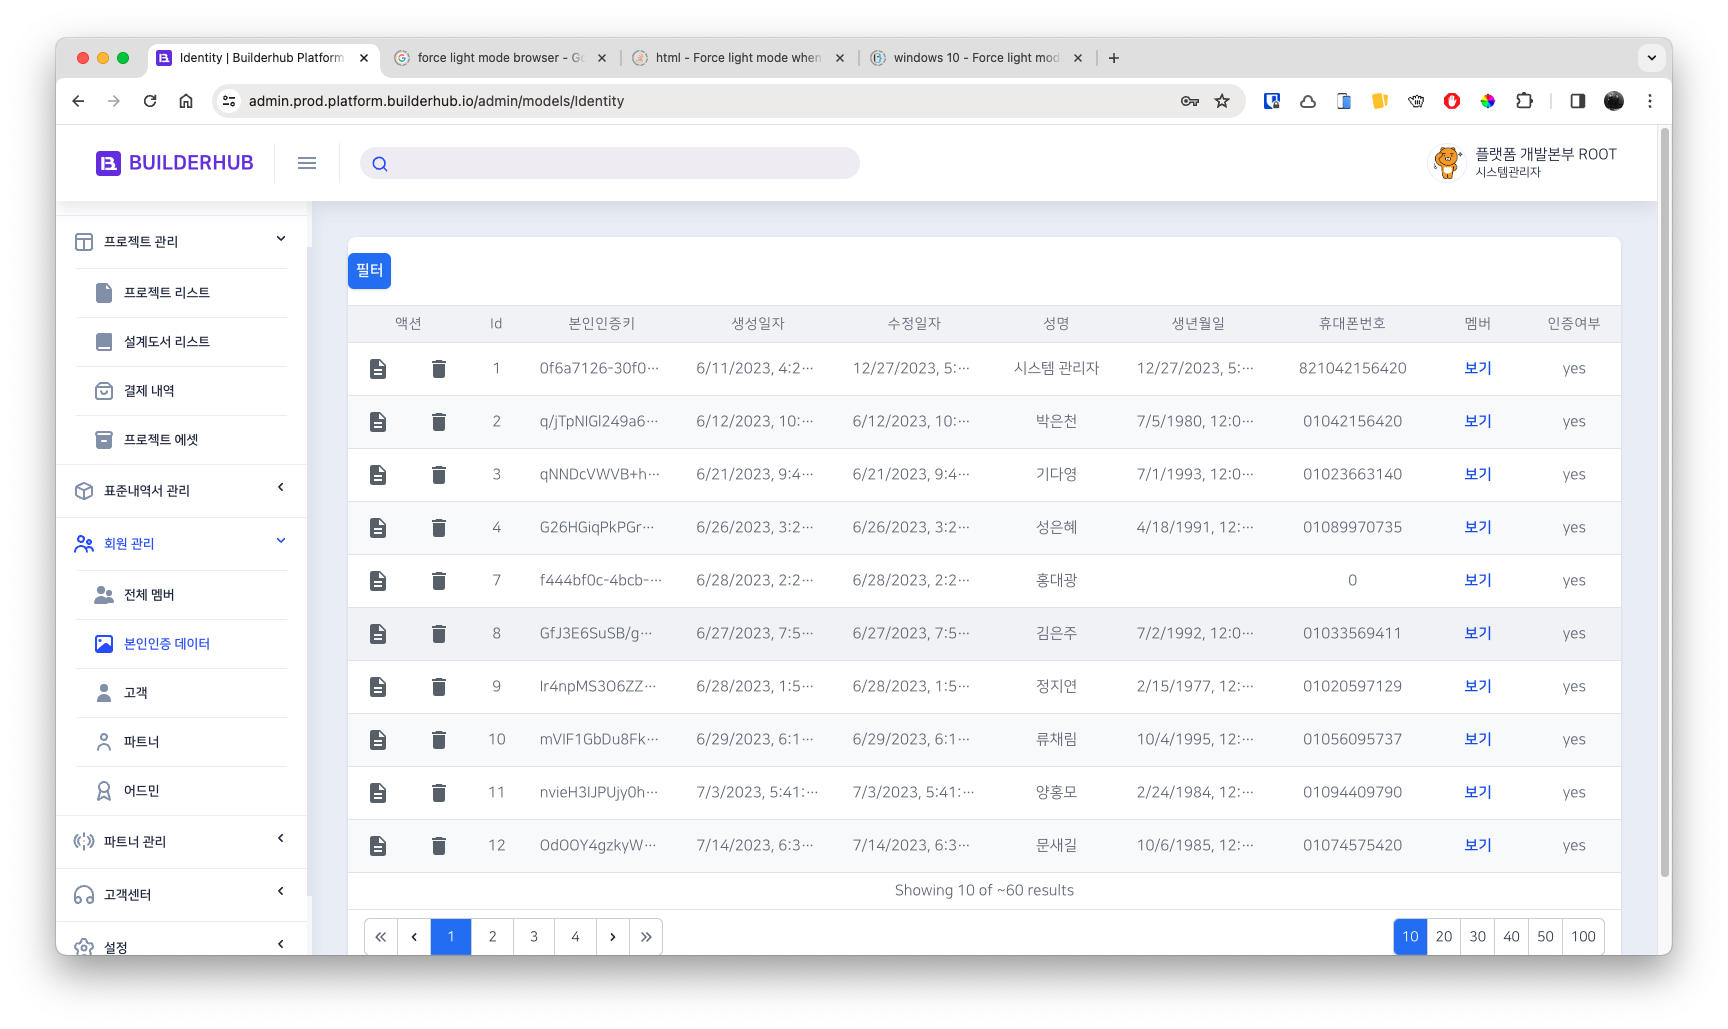
\includegraphics[width=0.35\textwidth]{images/builderhub-admin-member-identity.png}
				      \caption*{Member identity}
			      }\qquad
			      \parbox{0.35\textwidth}{
				      \centering
				      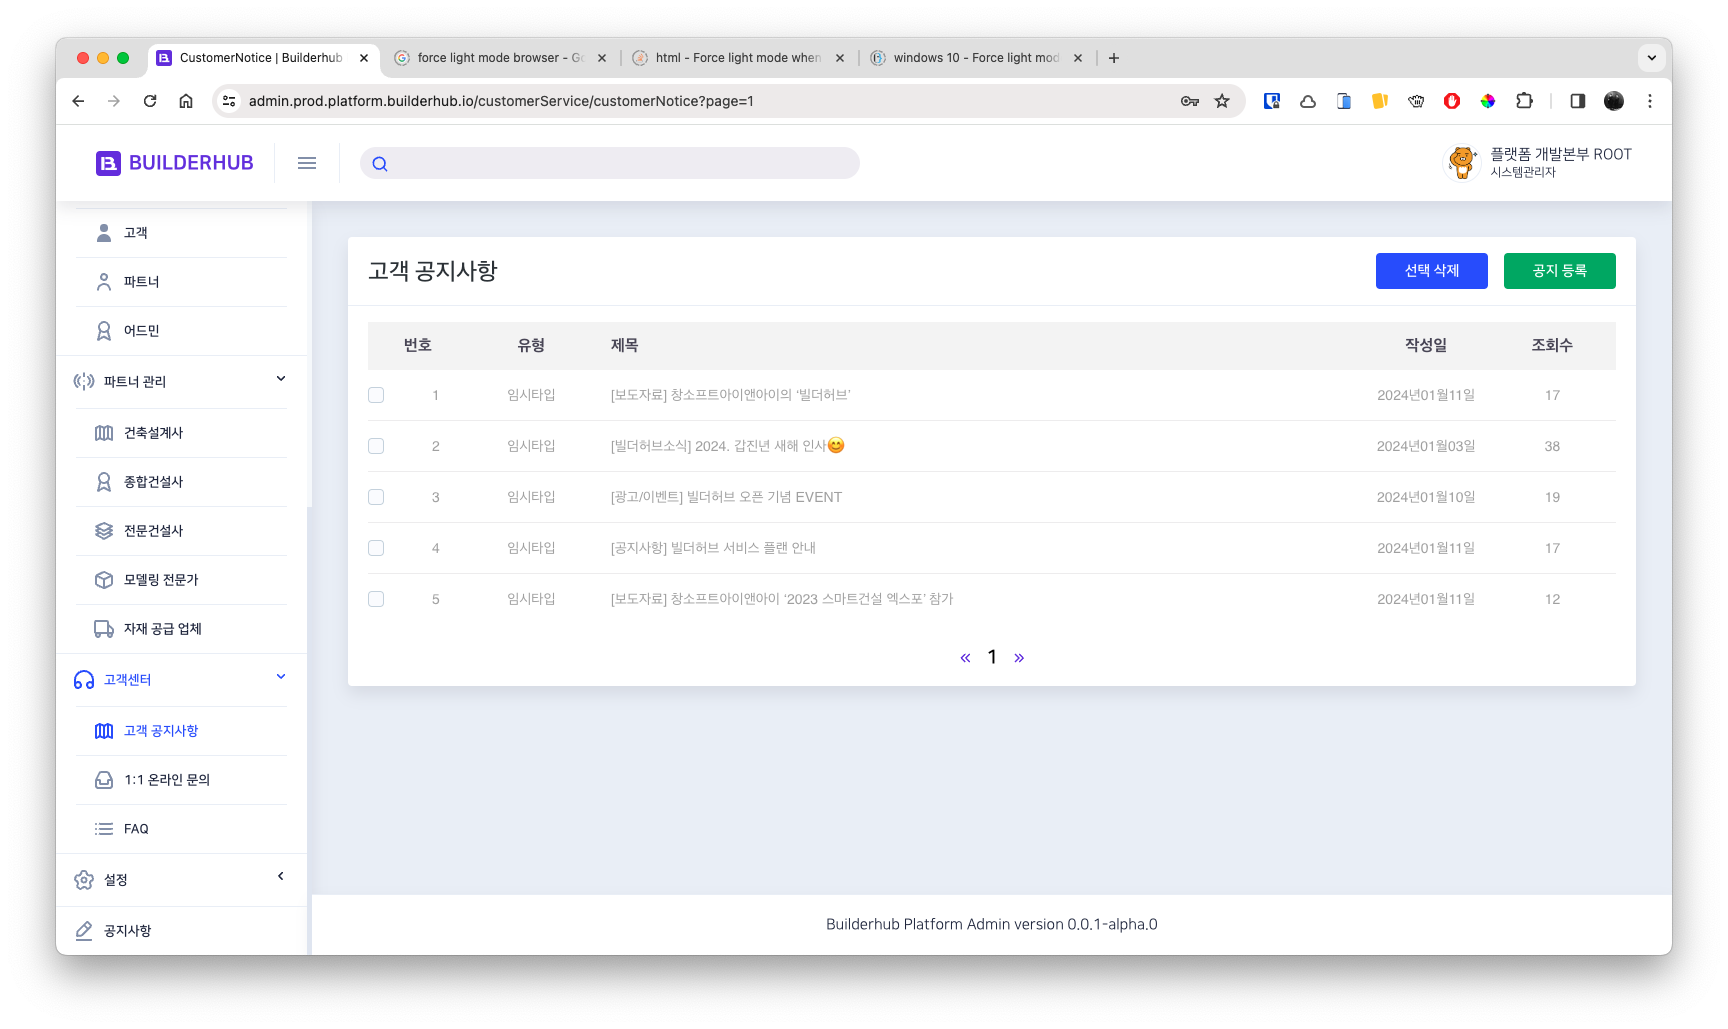
\includegraphics[width=0.35\textwidth]{images/builderhub-admin-notice.png}
				      \caption*{Notice}
			      }\qquad
			      \parbox{0.35\textwidth}{
				      \centering
				      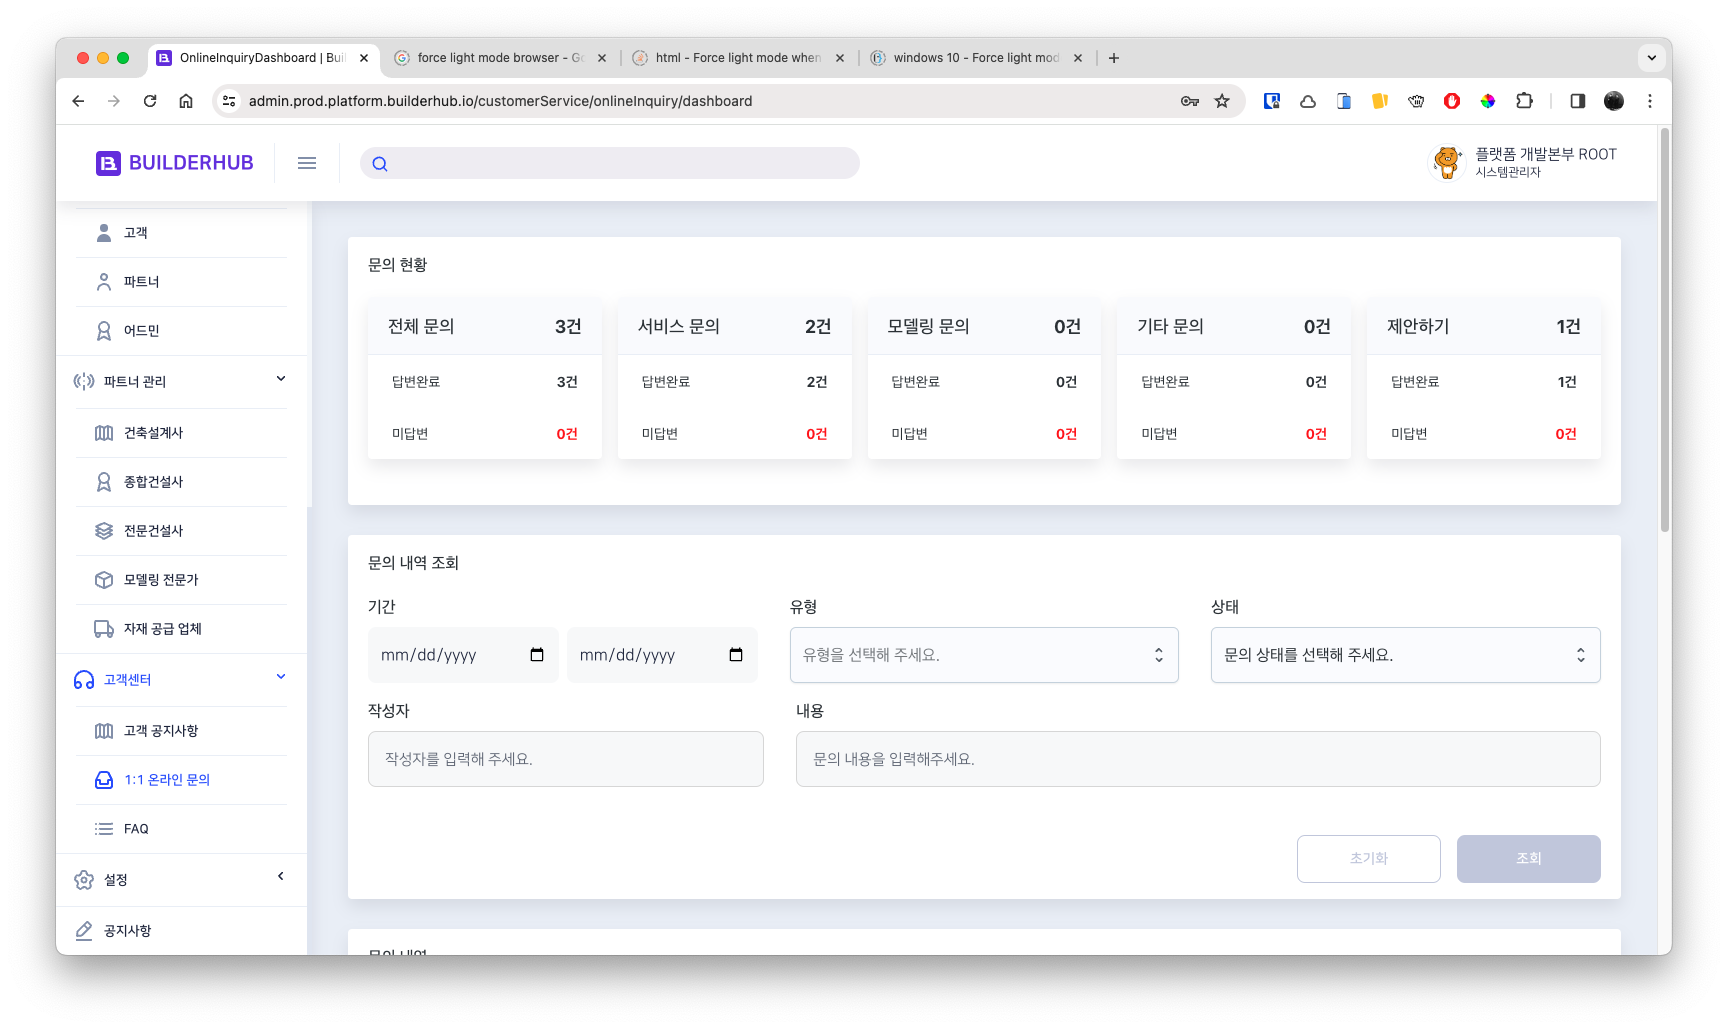
\includegraphics[width=0.35\textwidth]{images/builderhub-admin-one-to-one-qa.png}
				      \caption*{1:1 문의}
			      }\qquad
			      \parbox{0.35\textwidth}{
				      \centering
				      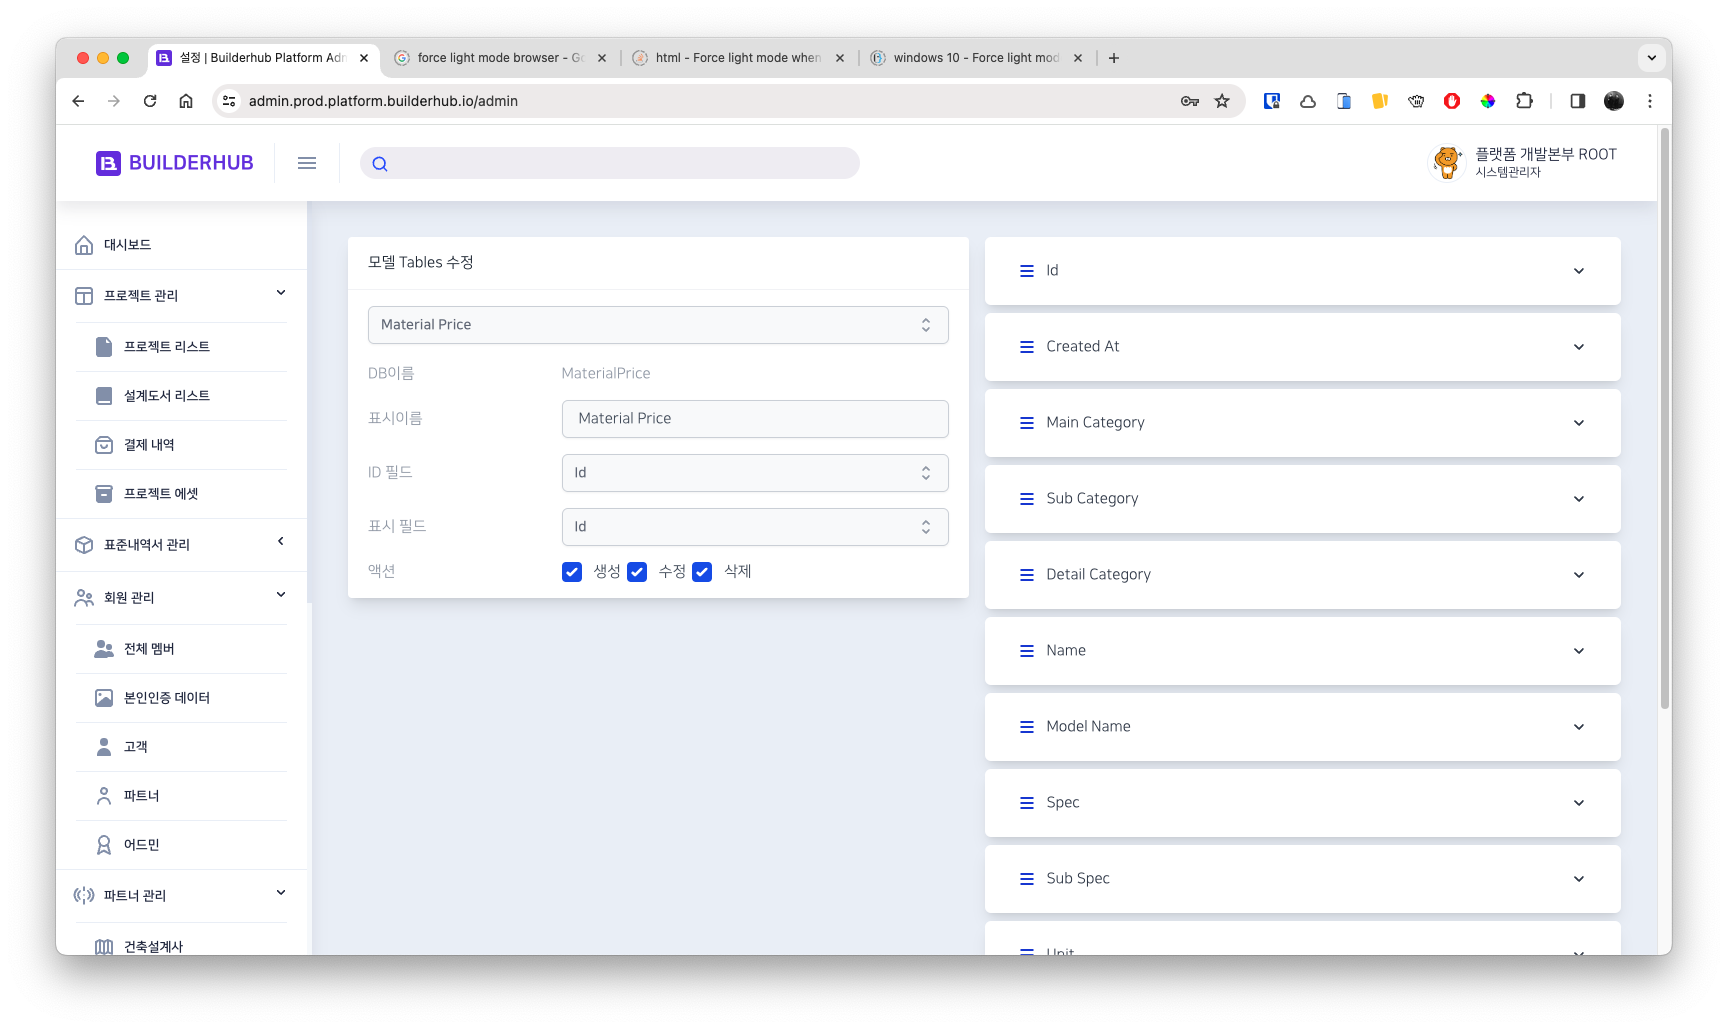
\includegraphics[width=0.35\textwidth]{images/builderhub-admin-settings.png}
				      \caption*{Settings}
			      }
		      \end{fullwidth}
	      \end{figure}
	\item 플랫폼 컨버터 개발
	      \begin{itemize}
		      \item 솔루션 데이터 프리프로세싱, 디폴트 값 추가
		      \item 비내역화 데이터 계산 및 추가, 표준내역서 매핑, 공사비 데이터 매핑 및 공사비 산출
		      \item 솔루션 BIM 모델데이터 업로드 및 변환
		      \item 개발 스택: TypeScript, NodeJS, ElectronJS, NextJS(Nextron), Default data and Validator(AJV), CSV Parser(papaparse)
	      \end{itemize}
	      \begin{figure}[!ht]
		      \begin{fullwidth}
			      \parbox{0.45\textwidth}{
				      \centering
				      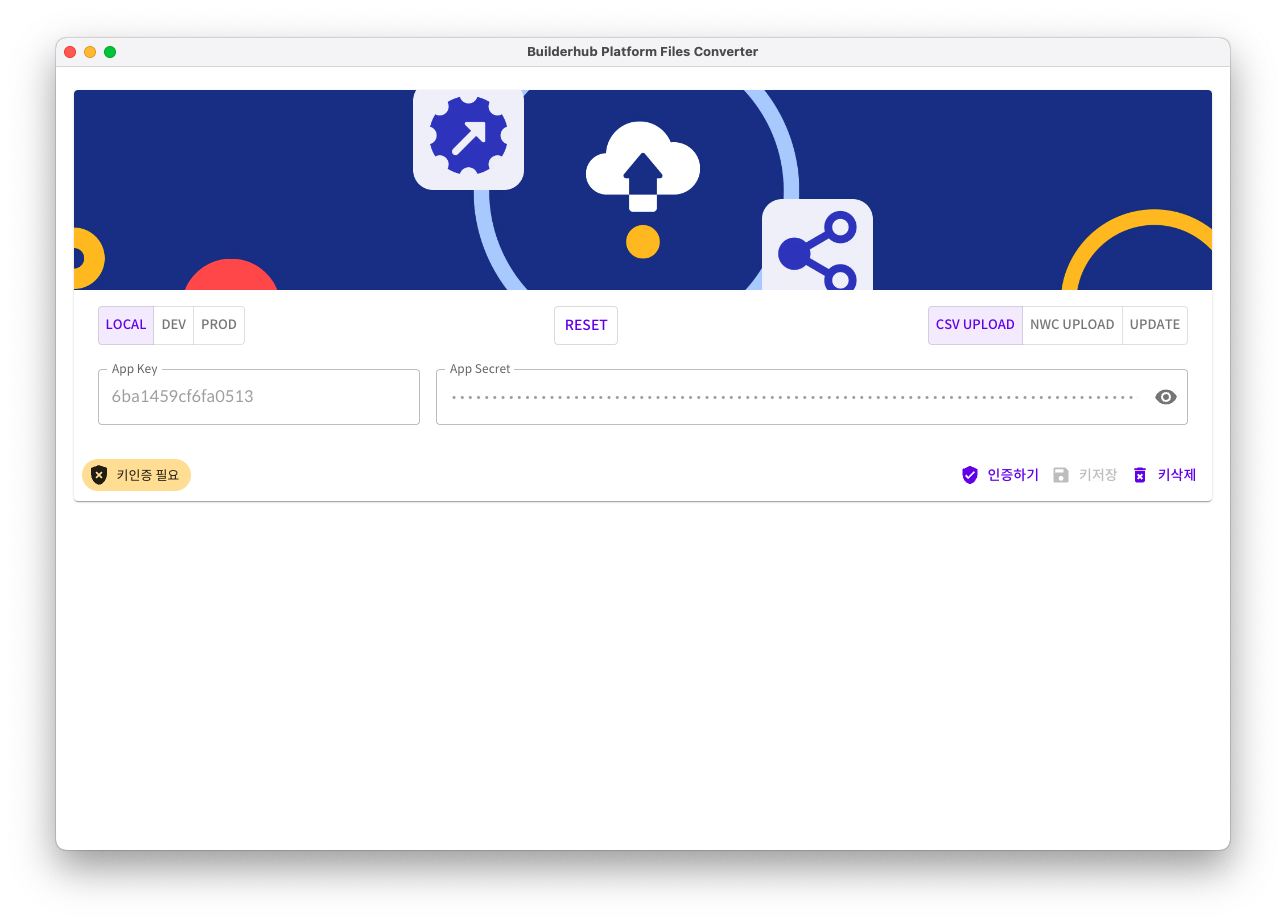
\includegraphics[width=0.28\textwidth]{images/builderhub-converter-main.png}
				      \caption*{Main}
			      }\qquad
			      \parbox{0.45\textwidth}{
				      \centering
				      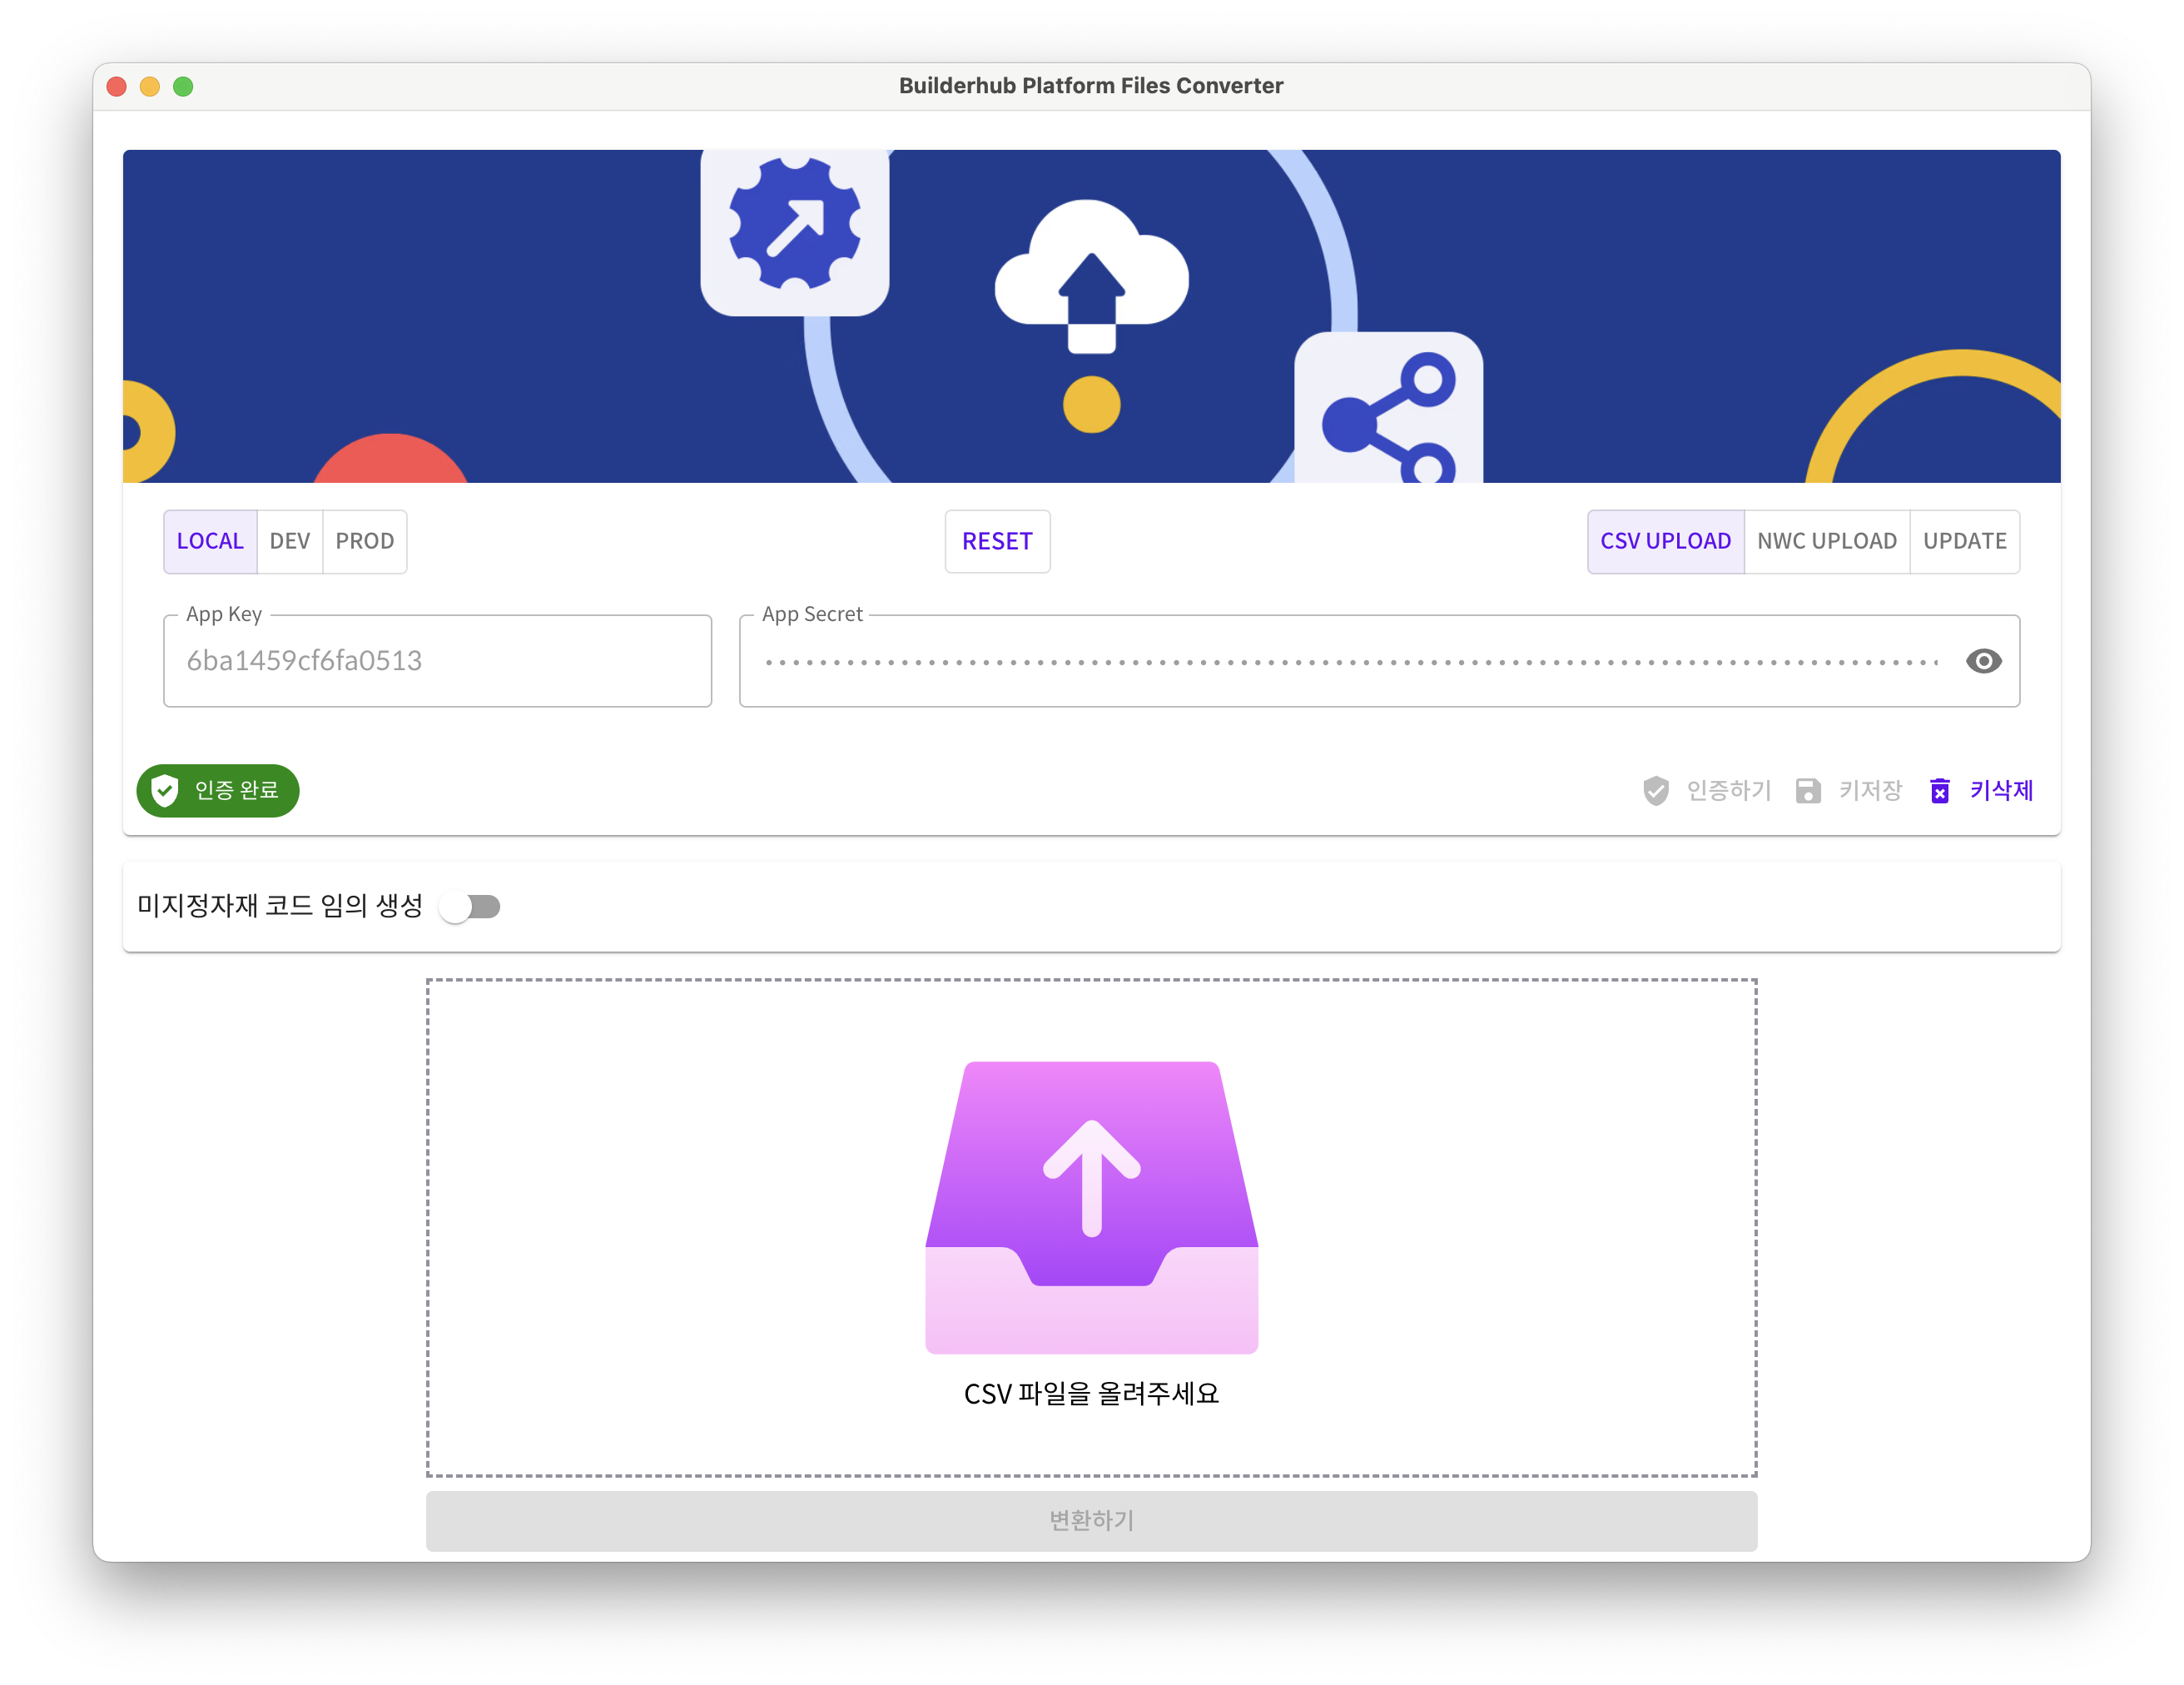
\includegraphics[width=0.25\textwidth]{images/builderhub-converter-auth.png}
				      \caption*{Authorized}
			      }\qquad
			      \parbox{0.45\textwidth}{
				      \centering
				      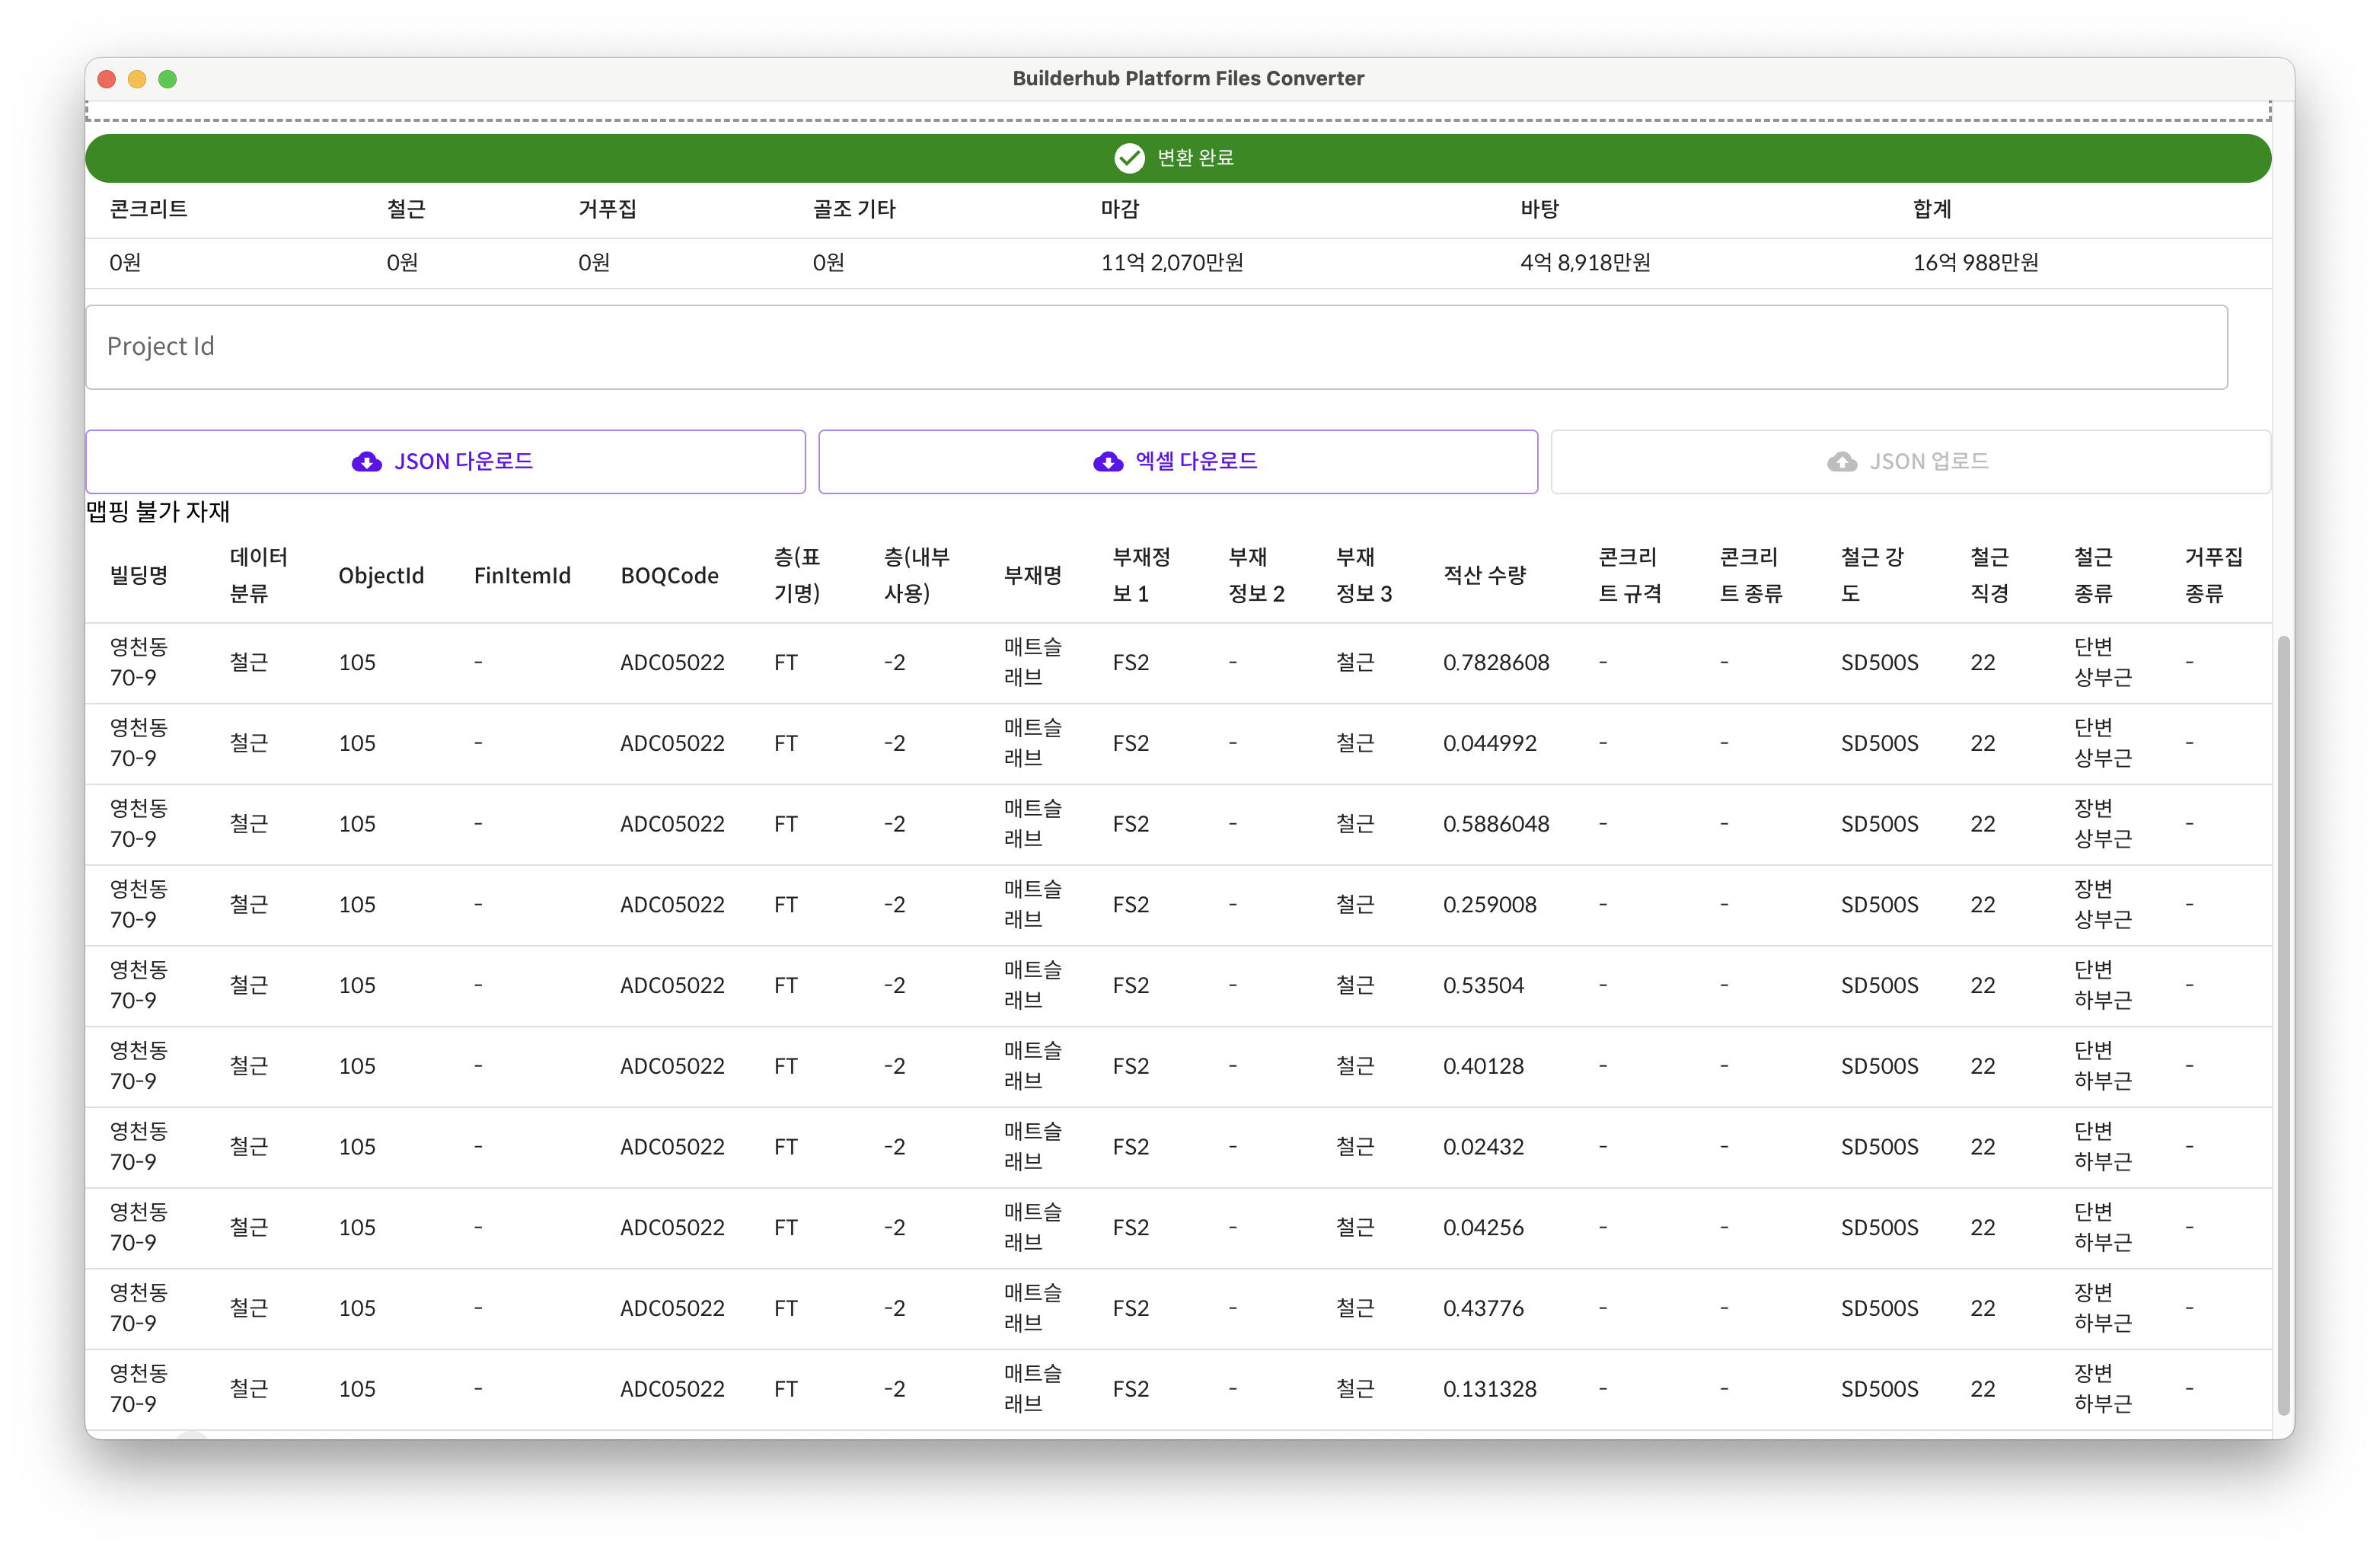
\includegraphics[width=0.28\textwidth]{images/builderhub-converter-converted.png}
				      \caption*{Converted: Mapping}
			      }
		      \end{fullwidth}
	      \end{figure}
	\item 인프라 구성:
	      \begin{itemize}
		      \item 1차 코드형 인프라(IaC: AWS Copilot, AWS CDK 2022.06 - 2022.10): AWS CloudFormation, Amplify, Cognito, ALB, RDS, Lambda, API Gateway, S3, CloudFront
		      \item 2차 코드형 인프라(IaC: Terraform 2022.11 - 2023.12): AWS ECS, RDS, Lambda, API Gateway, S3, CloudFront, SES 등
		      \item 3차 쿠버네티스 인프라(IaC: Terraform, Helm Chart 2023.12 - now): EKS, ELB, PostgreSQL, Prometheus, Grafana, ArgoCD, Github Action, Nginx, Supertokens 등
	      \end{itemize}
	      \begin{figure}[!ht]
		      \begin{fullwidth}
			      \parbox{0.8\textwidth}{
				      \centering
				      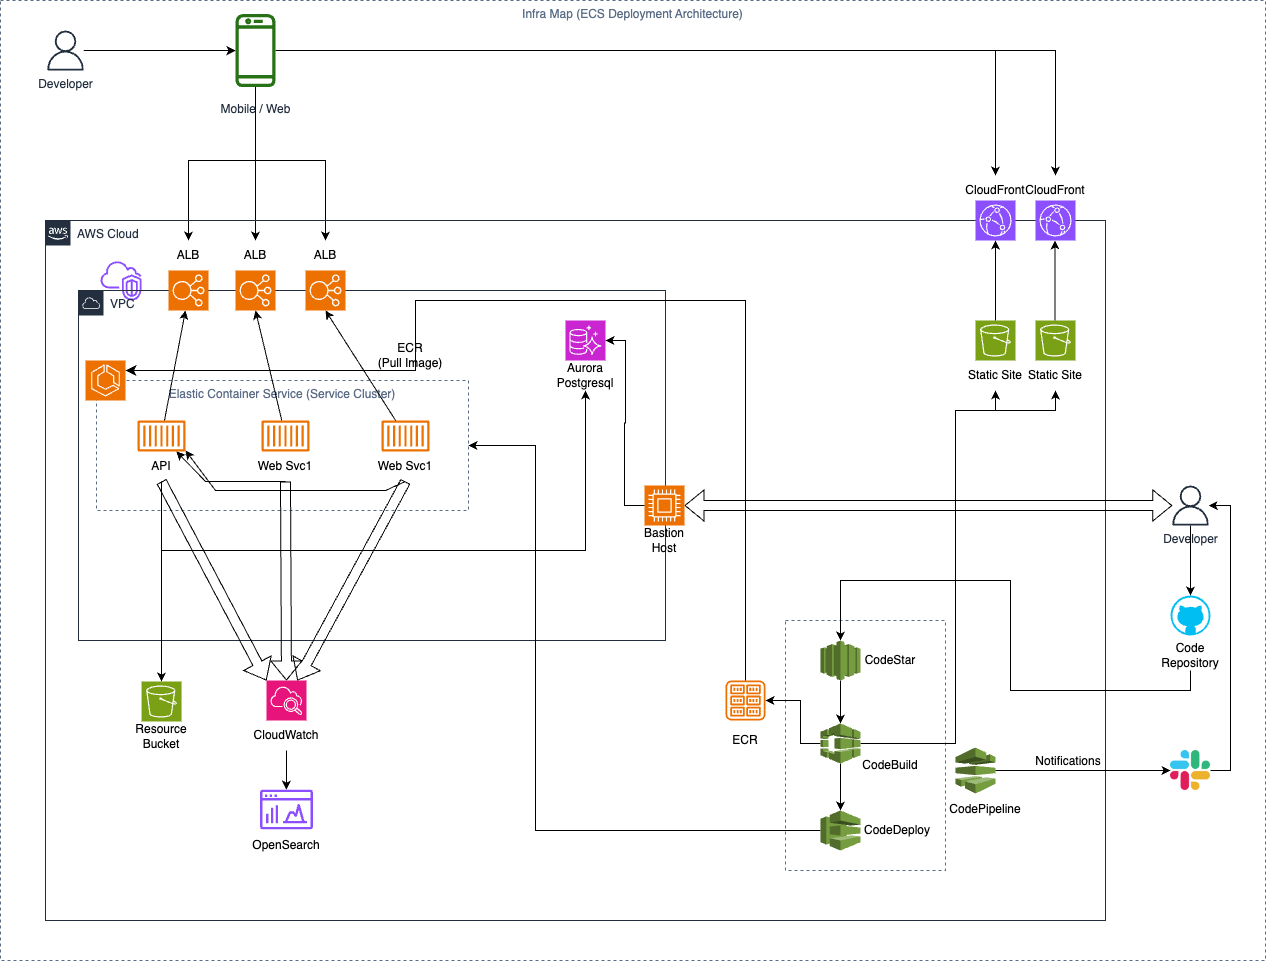
\includegraphics[width=0.40\textwidth]{images/ECS Architecture (bg_white).png}
				      \caption*{ECS Infra}
			      }\qquad
			      \parbox{0.6\textwidth}{
				      \centering
				      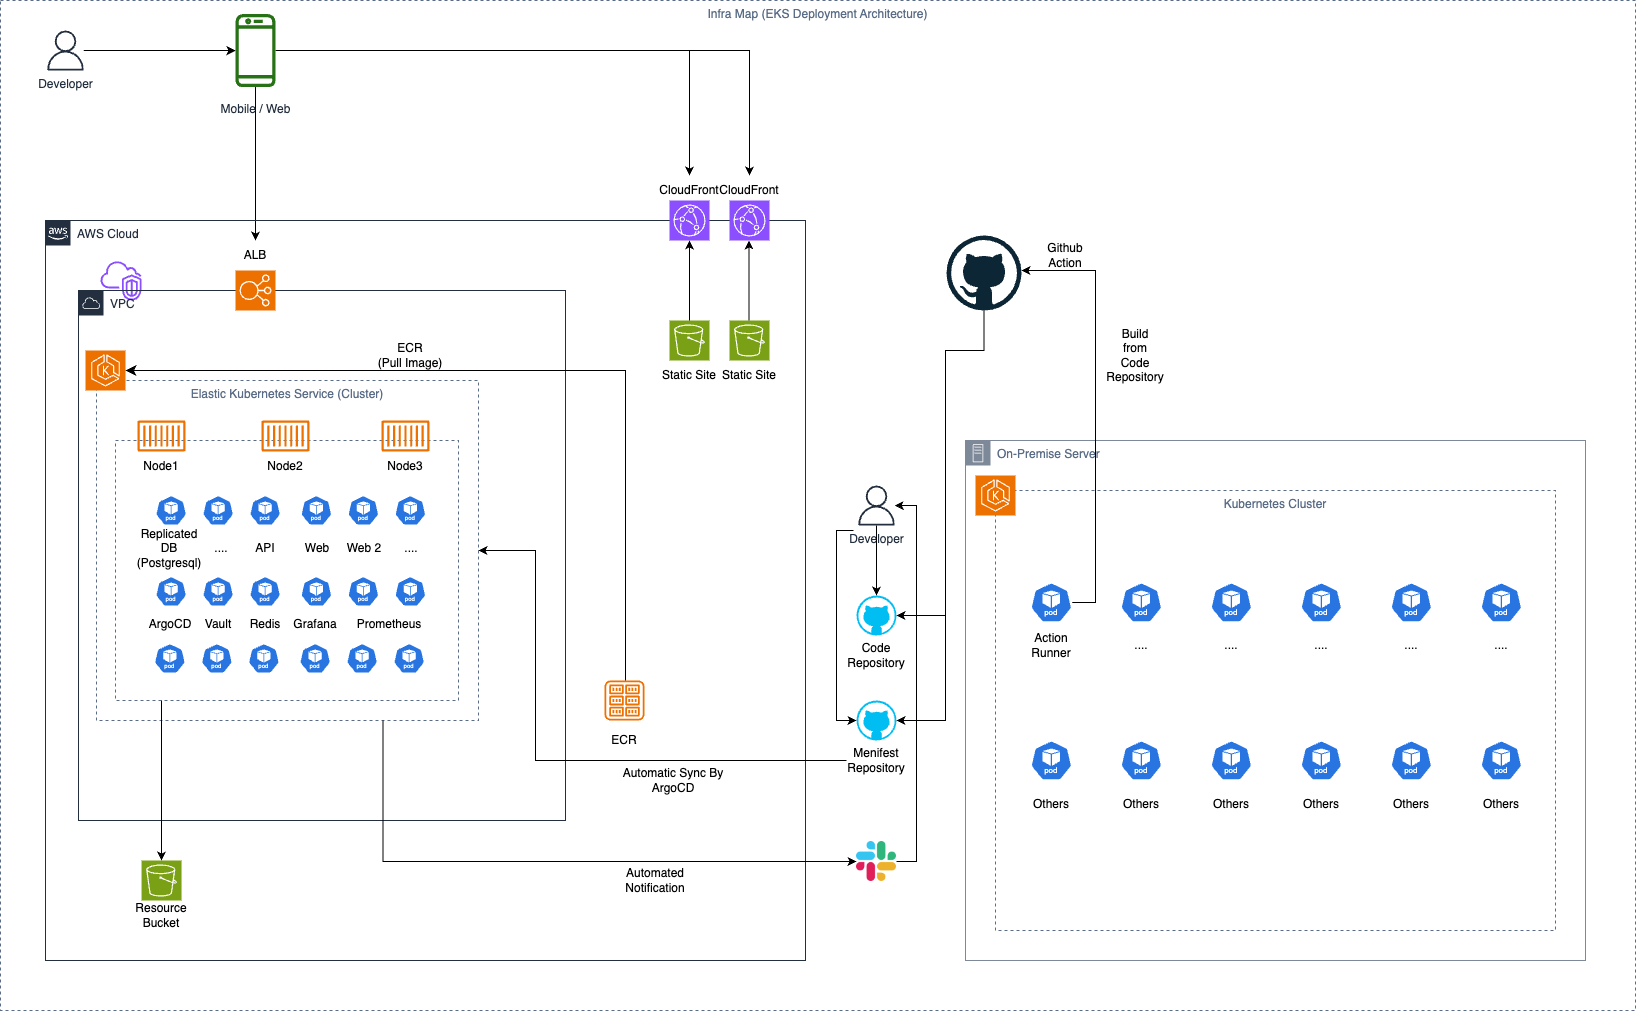
\includegraphics[width=0.5\textwidth]{images/EKS Architecture (bg_white).png}
				      \caption*{EKS Infra}
			      }
		      \end{fullwidth}
	      \end{figure}
	\item 백엔드 개발 스택: TypeScript, NodeJS, Apollo Server, Code first GraphQL Schema, GraphQL Codegen, Nexus Framework, PalJS, OAS REST API 등
	\item 프론트엔드 개발 스택: TypeScript, NextJS, ReactJS, Redux toolkit, XState, Threejs, Autodesk Forge SDK
\end{itemize}

\cvevent{\printinfo{\faPlusSquare}{스마트체커 개발(B2B)}}{(주)창소프트아이앤아이 개발리딩}{2023.09 -- now}{Seoul, Korea}

\begin{itemize}
	\item \href{https://check.builderhub.io/signin}{스마트체커}(철근 모니터링 시스템, 시공사 대상 B2B) 프로젝트 개발
	      \begin{itemize}[label=$\star$]
		      \item 개발 기간: 3개월
		      \item 개발 인원: 4명
		      \item 개발한 서비스
		            \begin{itemize}
			            \item 스마트체커 서비스: 자사 솔루션 제품 데이터(Builderhub Q, 2DShopPro)를 활용한 철근 물량 검토 서비스
			            \item 파일클라우드: 웹하드 대체를 위한 파일클라우드 개발
			            \item 이슈 트래킹: 도면 또는 자체 이슈들을 관리하기 위한 이슈관리 서비스 개발
			            \item 도면 컨버터 개발: 철근 샵도면을 읽어 물량 정보 및 메타데이터를 추출 및 도면 뷰어를 위한 데이터 컨버팅
		            \end{itemize}
		            \begin{figure}[!ht]
			            \begin{fullwidth}
				            \parbox{0.35\textwidth}{
					            \centering
					            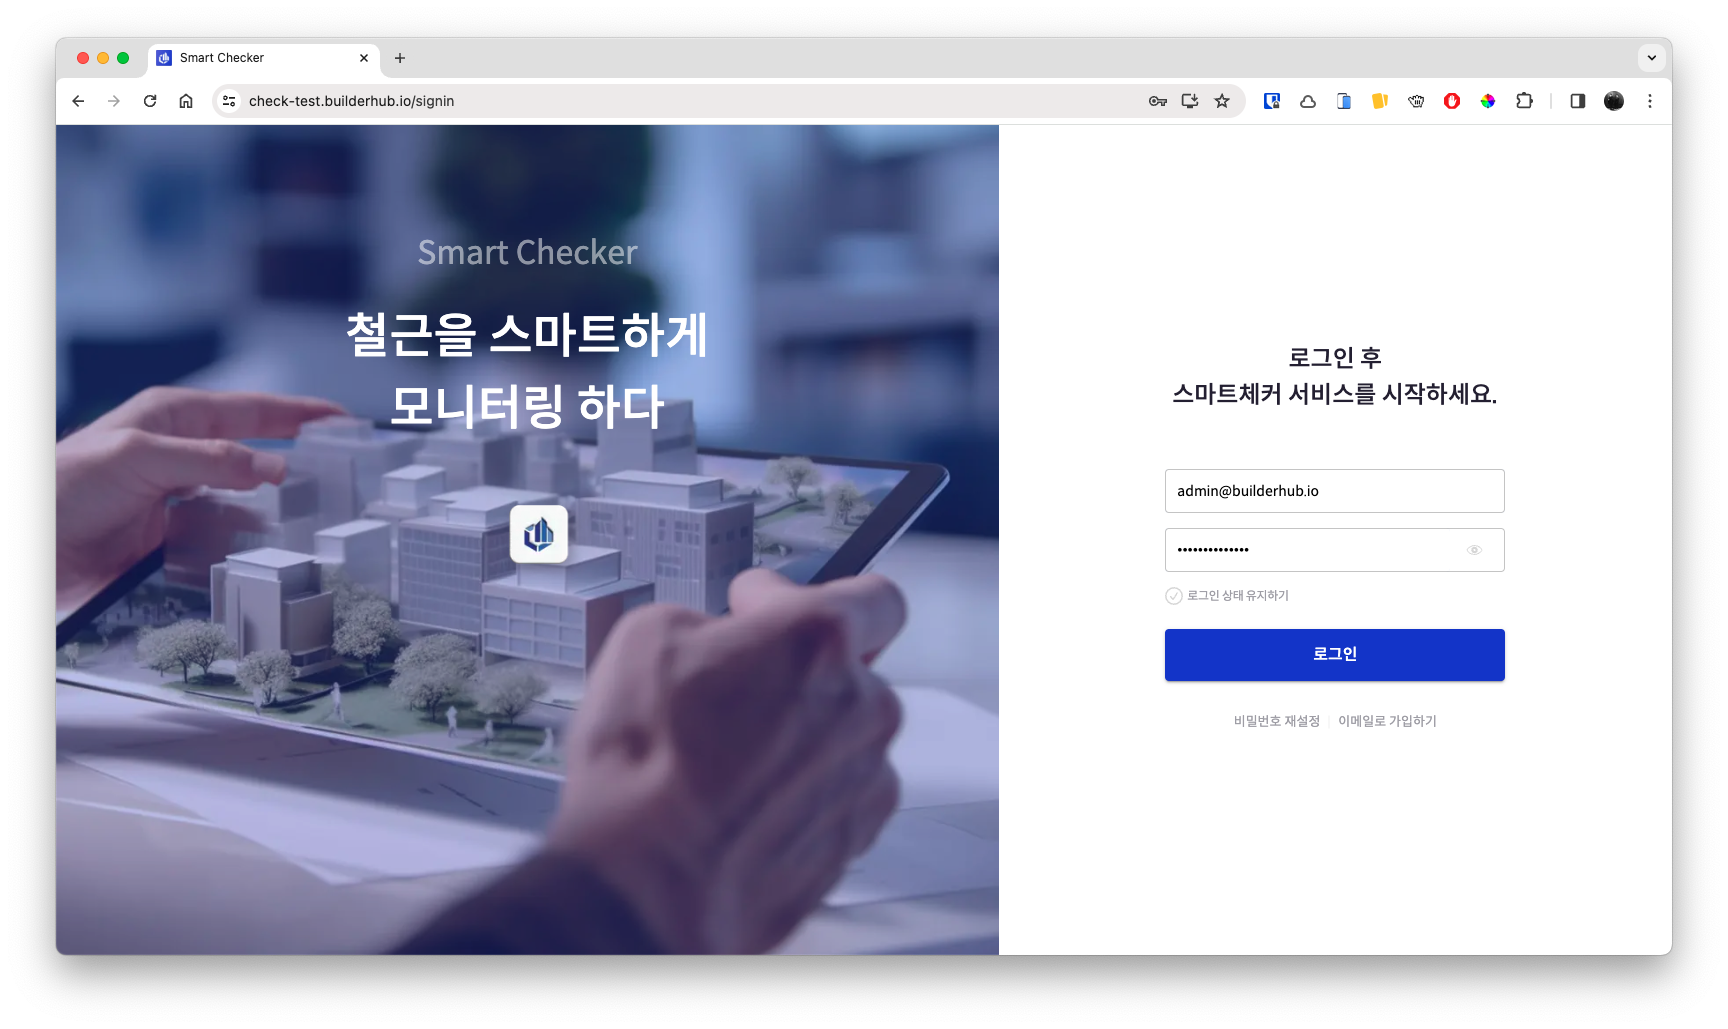
\includegraphics[width=0.35\textwidth]{images/smart-checker-auth.png}
					            \caption*{Authentication}
				            }\qquad
				            \parbox{0.35\textwidth}{
					            \centering
					            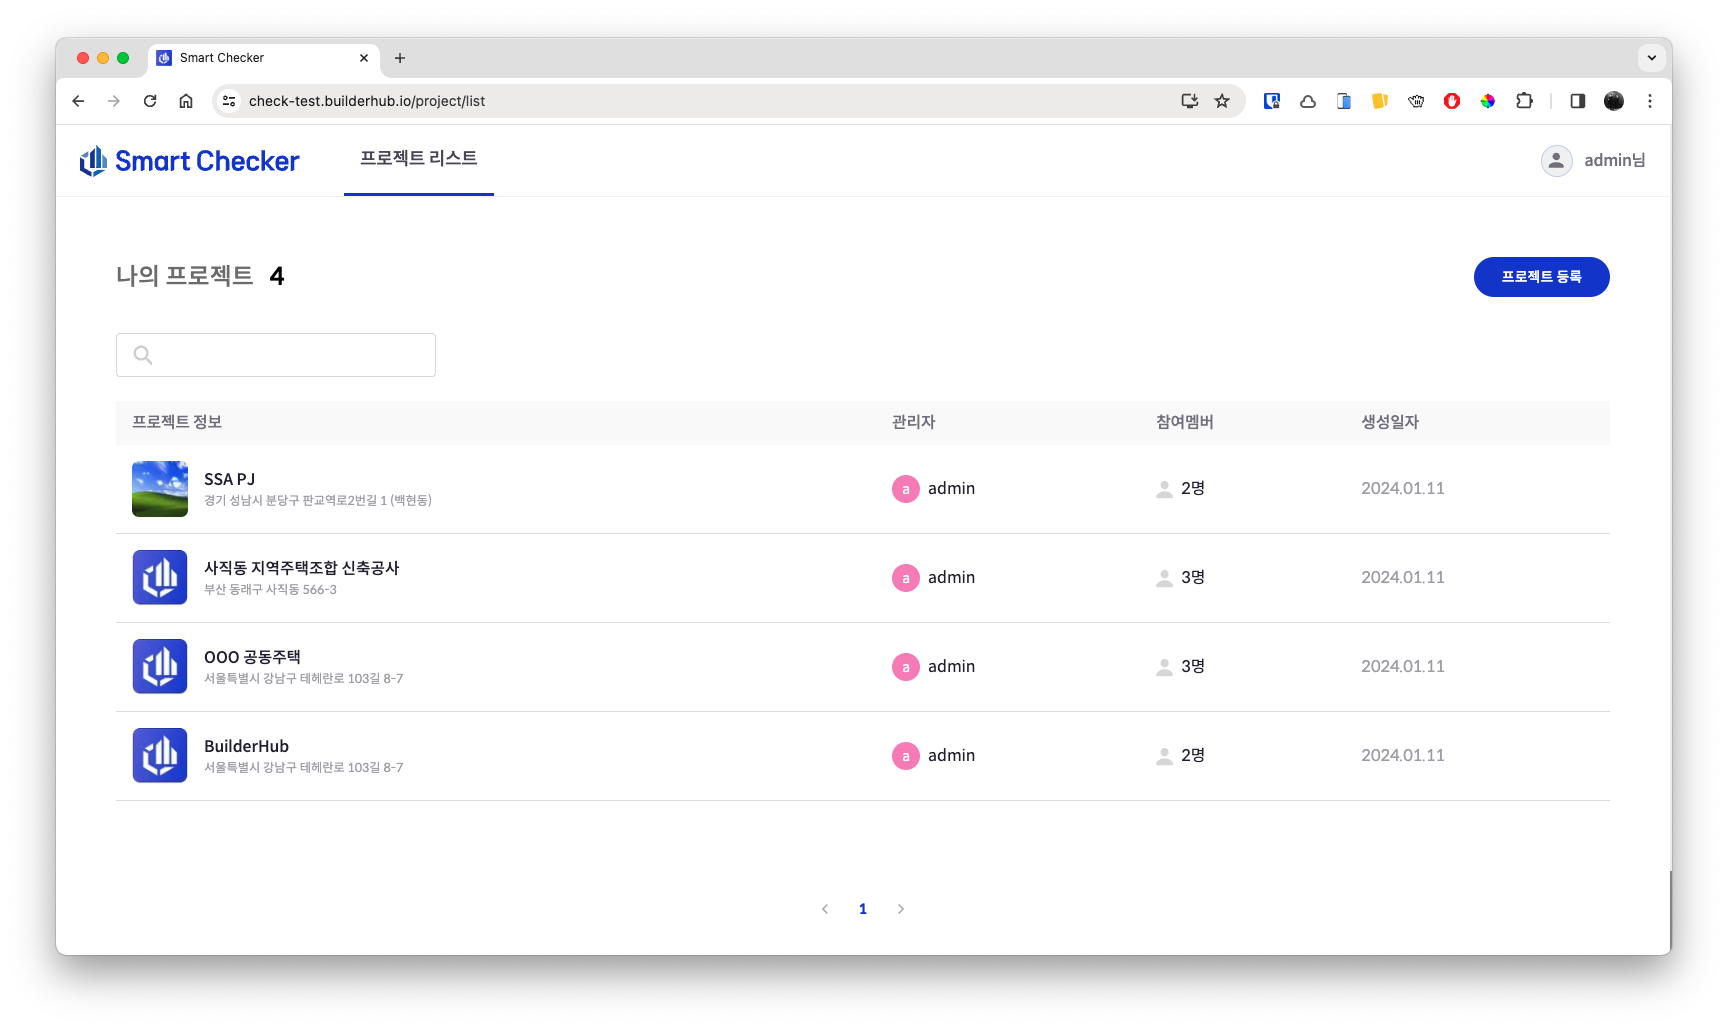
\includegraphics[width=0.35\textwidth]{images/smart-checker-project-list.png}
					            \caption*{Project list}
				            }\qquad
				            \parbox{0.35\textwidth}{
					            \centering
					            \includegraphics[width=0.35\textwidth]{images/smart-checker-project-info.png}
					            \caption*{Project information}
				            }\qquad
				            \parbox{0.35\textwidth}{
					            \centering
					            \includegraphics[width=0.35\textwidth]{images/smart-checker-csv-upload.png}
					            \caption*{CSV upload(BH-Q)}
				            }
				            \parbox{0.35\textwidth}{
					            \centering
					            \includegraphics[width=0.35\textwidth]{images/smart-checker-csv-upload-pivot.png}
					            \caption*{물량 Chart, 피벗테이블}
				            }\qquad
				            \parbox{0.35\textwidth}{
					            \centering
					            \includegraphics[width=0.35\textwidth]{images/smart-checker-dashboard.png}
					            \caption*{Dashboard}
				            }\qquad
				            \parbox{0.35\textwidth}{
					            \centering
					            \includegraphics[width=0.35\textwidth]{images/smart-checker-approval-status.png}
					            \caption*{시공사 승인현황}
				            }\qquad
				            \parbox{0.35\textwidth}{
					            \centering
					            \includegraphics[width=0.35\textwidth]{images/smart-checker-file-browser.png}
					            \caption*{클라우드 파일 관리}
				            }
			            \end{fullwidth}
		            \end{figure}
		      \item 인프라 구성:
		            \begin{itemize}
			            \item 쿠버네티스 인프라 구성: EKS, ELB, Prometheus, Grafana, ArgoCD, Github Action, Nginx, Supertokens 등
			            \item Turbo Repo 구성: 모노 리포지토리에서 모든 앱과 패키지들을 통합하여 관리 및 배포
		            \end{itemize}
		      \item 백엔드 \& 프론트 개발 스택: TypeScript, NodeJS, Apollo Server, Code first GraphQL Schema, GraphQL Codegen, Nexus Framework, PalJS, OAS REST API, NextJS
	      \end{itemize}

	      \begin{figure}[!ht]
		      \begin{fullwidth}
			      \parbox{0.35\textwidth}{
				      \centering
				      \includegraphics[width=0.35\textwidth]{images/smart-checker-admin-project-list.png}
				      \caption*{어드민: Project List}
			      }\qquad
			      \parbox{0.35\textwidth}{
				      \centering
				      \includegraphics[width=0.35\textwidth]{images/smart-checker-admin-license-list.png}
				      \caption*{어드민: 발급 라이센스}
			      }\qquad
			      \parbox{0.35\textwidth}{
				      \centering
				      \includegraphics[width=0.35\textwidth]{images/smart-checker-admin-license-generation.png}
				      \caption*{어드민: 라이센스 발급}
			      }\qquad
			      \parbox{0.35\textwidth}{
				      \centering
				      \includegraphics[width=0.35\textwidth]{images/smart-checker-admin-org-list.png}
				      \caption*{어드민: 업체 리스트}
			      }
			      \parbox{0.35\textwidth}{
				      \centering
				      \includegraphics[width=0.35\textwidth]{images/smart-checker-sd-upload-chart.png}
				      \caption*{샵도면 업로드 및 골구도차트}
			      }\qquad
			      \parbox{0.35\textwidth}{
				      \centering
				      \includegraphics[width=0.35\textwidth]{images/smart-checker-sd-listing.png}
				      \caption*{샵도면 리스트 및 변환}
			      }\qquad
			      \parbox{0.35\textwidth}{
				      \centering
				      \includegraphics[width=0.35\textwidth]{images/smart-checker-approval.png}
				      \caption*{샵업체 승인현황}
			      }\qquad
			      \parbox{0.35\textwidth}{
				      \centering
				      \includegraphics[width=0.35\textwidth]{images/smart-checker-my-page.png}
				      \caption*{회원 마이페이지}
			      }
		      \end{fullwidth}
	      \end{figure}
\end{itemize}

\cvevent{\printinfo{\faPlusSquare}{건축 감리 B2B 프로젝트 개발: \href{https://asec.builderhub.io/dashboard/detail/initial/supervision}{DEMO}}}{(주)창소프트아이앤아이}{2023.10 -- 2023.11}{Seoul, Korea}

\begin{itemize}[label=$\star$]
	\item 개발 기간: 3주
	\item 개발 인원: 2명
	\item 개발한 서비스
	      \begin{itemize}
		      \item 건축 공정표와 공정 체크리스트, 모델 연동, 공장 가공 철근 부재별 체크하여 사진 업로드
		      \item URL에 해당 데이터 저장 및 S3 이미지 업로드, URL Shortener, 공장 가공 철근 QR Code 연동
	      \end{itemize}
\end{itemize}
\begin{figure}[!ht]
	\begin{fullwidth}
		\parbox{0.35\textwidth}{
			\centering
			\includegraphics[width=0.35\textwidth]{images/builderhub-supervision-landing-1.png}
			\caption*{Landing page}
		}\qquad
		\parbox{0.35\textwidth}{
			\centering
			\includegraphics[width=0.35\textwidth]{images/builderhub-supervision-project-list.png}
			\caption*{Project list}
		}\qquad
		\parbox{0.35\textwidth}{
			\centering
			\includegraphics[width=0.35\textwidth]{images/builderhub-supervision-main-1.png}
			\caption*{Supervision}
		}\qquad
		\parbox{0.35\textwidth}{
			\centering
			\includegraphics[width=0.35\textwidth]{images/builderhub-supervision-checklist.png}
			\caption*{Check list}
		}
		\parbox{0.35\textwidth}{
			\centering
			\includegraphics[width=0.35\textwidth]{images/builderhub-supervision-check-member.png}
			\caption*{Member check}
		}\qquad
		\parbox{0.35\textwidth}{
			\centering
			\includegraphics[width=0.35\textwidth]{images/builderhub-supervision-asec.png}
			\caption*{ASEC Check main}
		}\qquad
		\parbox{0.35\textwidth}{
			\centering
			\includegraphics[width=0.35\textwidth]{images/builderhub-supervision-asec-model-check.png}
			\caption*{ASEC Model check}
		}\qquad
		\parbox{0.35\textwidth}{
			\centering
			\includegraphics[width=0.35\textwidth]{images/builderhub-supervision-archi-gantt.png}
			\caption*{Architecture milestones}
		}
	\end{fullwidth}
\end{figure}
